\documentclass[11pt,twoside,a4paper,openright]{uclouvain-thesis}

\usepackage[left=4.5cm,right=4.5cm,top=4.8cm,bottom=4.8cm]{geometry}

\usepackage{../../latex/custom}
\usepackage{../../latex/jsr}
\usepackage{../../latex/nsi}
\renewcommand{\tEc}{Entropic Cone}
\usepackage{../../latex/mythm_pre}

\usepackage[utf8]{inputenc}
\usepackage{csquotes}

\usepackage{pifont}
\newcommand{\cmark}{\ding{51}}%
\newcommand{\xmark}{\ding{55}}%

\newif\ifnotnotes
\notnotestrue


\newenvironment{notationlist}[1]
{\vspace{1em}

\noindent
\textbf{#1}:


\begin{longtable}{p{0.5\textwidth}p{0.48\textwidth}}}
{\end{longtable}}

\usepackage{comment}
\usepackage{siunitx}

\usepackage[]{minted}
\usepackage{tcolorbox}
\usepackage{etoolbox}
\BeforeBeginEnvironment{minted}{\begin{tcolorbox}}%
\AfterEndEnvironment{minted}{\end{tcolorbox}}

\usepackage{tkz-graph}
\usepackage{tikz}
\usetikzlibrary{arrows,matrix,decorations.pathreplacing,positioning,chains,fit,shapes,calc} %
\usetikzlibrary{calc,patterns,decorations.pathmorphing,decorations.markings}
\usepackage{pgfplots}

\usepackage[style=alphabetic,maxbibnames=99,giveninits=true]{biblatex}
\addbibresource{biblio.bib}

\preto\fullcite{\AtNextCite{\defcounter{maxnames}{99}}}
\AtEveryBibitem{%
	\clearlist{language}
	\ifentrytype{online}{}{%
		\clearfield{url}
		\clearfield{urldate}
	}
}

\DeclareBibliographyCategory{fullcited}
\newcommand{\mybibexclude}[1]{\addtocategory{fullcited}{#1}}
\newcommand{\myfullcite}[1]{\fullcite{#1}.\mybibexclude{#1}}

\usepackage[ttscale=.875]{libertine}
\usepackage[libertine]{newtxmath}

\usepackage{datetime}



\usepackage[font=small]{caption}
\captionsetup[figure]{labelfont=bf,textfont=bf}
\captionsetup[table]{labelfont=bf,textfont=bf}
\usepackage{subcaption}

\usepackage{float}

\usepackage{mdframed}

\usepackage{fancyvrb}

\usepackage{xspace}

\usepackage{textcomp}

\usepackage{pbox}
\usepackage[clearempty,newlinetospace,raggedright,small,explicit]{titlesec}

\definecolor{gray65}{gray}{0.65}

\newcommand{\size}[2]{{\fontsize{#1}{0}\selectfont #2}}
\newcommand{\sizeline}[3]{{\fontsize{#1}{#2}\selectfont #3}}
\newenvironment{sizepar}[2]
{\par\fontsize{#1}{#2}\selectfont}
{\par}

\newcommand{\printchapternumber}{%
	\begingroup\renewcommand{\arraystretch}{0}%
	\begin{tabular}{@{}c@{}}\size{56}{\thechapter}\end{tabular}%
	\endgroup
}

\titleformat{\chapter}[block]
{\bfseries\filright}
{}
{0pt}
{%
	\parbox{.865\textwidth}{\raggedright\Huge\selectfont#1}%
	\hspace{6pt}%
	\color{gray65}\vrule width 1.5pt
	\hspace{6pt}%
	\printchapternumber
}

\titleformat{name=\chapter,numberless}[block]
{\bfseries\filright}
{}
{0pt}
{%
	\parbox{\textwidth}{\raggedright\Huge\selectfont#1}%
}

\titlespacing*{\chapter}{0pt}{0pt}{60pt}

\newdateformat{monthyeardate}{\monthname[\THEMONTH] \THEYEAR}

\newcommand{\thesisTitle}{Set Programming: Theory and Computation}

\newcommand{\thesisAuthor}{Beno\^it Legat\xspace}

\newcommand{\clearemptydoublepage}{%
	\newpage{\pagestyle{empty}\cleardoublepage}}




\DeclareDatafieldSet{setall}{
  \member[datatype=literal]
  \member[datatype=name]
  \member[field=journal]%
}

\DeclareSourcemap{
  \maps[datatype=bibtex]{
    \map[overwrite, foreach={setall}]{
      \step[fieldsource=\regexp{$MAPLOOP},
            match=\regexp{\x{0131}\x{0300}},
            replace=\regexp{\x{00EC}}]
      \step[fieldsource=\regexp{$MAPLOOP},
            match=\regexp{\x{0131}\x{0301}},
            replace=\regexp{\x{00ED}}]
      \step[fieldsource=\regexp{$MAPLOOP},
            match=\regexp{\x{0131}\x{0302}},
            replace=\regexp{\x{00EE}}]
      \step[fieldsource=\regexp{$MAPLOOP},
            match=\regexp{\x{0131}\x{0308}},
            replace=\regexp{\x{00EF}}]
    }
  }
}

\usepackage{mathtools}
\newcommand{\verteq}{\rotatebox{90}{$=$}}

\newcommand{\implementations}[1]{}
\newcommand{\Cset}{\mathcal{C}}

\DeclareMathOperator{\gauge}{g}
\DeclareMathOperator{\domain}{Dom}
\DeclareMathOperator{\Init}{Init}
\DeclareMathOperator{\Guard}{Guard}

\newcommand{\eqnum}{r}
\newcommand{\ineqnum}{s}

\newcommand{\tr}{\to}
\newcommand{\trs}[1][\sigma]{\tr_{#1}}

\newcommand{\nqu}{n_{q,u}}
\newcommand{\nqx}{n_{q,x}}

\newcommand{\signal}{signal}
\newcommand{\signals}{signals}

\newcommand{\polyset}[1][p]{\mathcal{P}_{#1}}

\newcommand{\Ps}{\mathcal{P}}
\newcommand{\U}{\mathcal{U}}
\newcommand{\sys}{S}
\newcommand{\dtahcs}{HCS}
\newcommand{\dtahas}{HAS}
\newcommand{\Paths}{\G_k}
\newcommand{\expfrac}[2]{#1/#2}
\newcommand{\Hsys}{Hybrid automaton}
\newcommand{\hsys}{hybrid automaton}
\newcommand{\hsyss}{hybrid automata}

\newcommand{\johnintm}{\beta}
\newcommand{\johnint}{\tilde{\johnintm}}

\newcommand{\piB}{\pi_{\Image(B)^\perp}}
\newcommand{\piBinv}{\pi_{\Image(B)^\perp}^{-1}}

\newcommand{\brackets}[1]{\ensuremath{ \left[ #1 \right] }}
\newcommand{\tuple}[1]{\ensuremath{ \left\langle #1 \right\rangle }}
\newcommand{\Lang}{\mathcal{L}}
\newcommand{\DLang}[1][k]{\Lang^{[#1]}}
\newcommand{\DPaths}[1][t]{\G_{#1}^{[k]}}
\newcommand{\Deb}[1][k]{\G^{[#1]}}
\newcommand{\LangAutom}[1][\G]{{#1}^*}
\newcommand{\syst}[1]{System~(\ref{#1})}
\newcommand{\Oracle}{\mathcal{O}}
\newcommand{\Cycles}[1][k]{\Paths[#1]^\circ}
\newcommand{\set}[1]{\ensuremath{ \left\{ #1 \right\}}}
\newcommand{\dert}[1]{\ensuremath{ \dot{#1} }}
\newcommand{\ddert}[1]{\ensuremath{ \ddot{#1} }}
\newcommand{\pargroup}[1]{\ensuremath{ \left( #1 \right)}}

\newcommand{\vectorOne}[1]{\brackets{%
\begin{matrix}
  #1
 \end{matrix}%
}}
\newcommand{\vectorTwo}[2]{\brackets{%
\begin{matrix}
  #1 \\
  #2
 \end{matrix}%
}}
\newcommand{\vectorFour}[4]{\brackets{%
\begin{matrix}
  #1 \\
  #2 \\
  #3 \\
  #4
 \end{matrix}%
}}

\DeclareUnicodeCharacter{3B1}{$\alpha$}
\DeclareUnicodeCharacter{3BC}{$\mu$}
\DeclareUnicodeCharacter{3BD}{$\nu$}
\DeclareUnicodeCharacter{2207}{$\nabla$}

\newenvironment{aligneq*}%
{
\begin{equation*}
\begin{aligned}
}{
\end{aligned}
\end{equation*}
}

\newenvironment{aligneq}%
{
\begin{equation}
\begin{aligned}
}{
\end{aligned}
\end{equation}
}



\begin{document}

\thispagestyle{empty}

\begin{center}
\vspace{0.5cm}
{\bf \huge \textsc \thesisTitle}\\
~\\
\vspace{0.5cm}
\large \thesisAuthor\\
\vspace{1cm}
{\em Thesis submitted in partial fulfillment of the requirements for\\
the Degree of Doctor in Applied Sciences}\\
\vspace{1cm}
June 2020\\
\vspace{1cm}
ICTEAM\\
Louvain School of Engineering\\
Universit\'{e} catholique de Louvain\\
Louvain-la-Neuve\\
Belgium\\
\end{center}

\vspace{6.5cm}

\noindent\underline{\bf Thesis Committee:}\\
\begin{tabular}{lr}
Pr.~Rapha\"el M. {\bf Jungers} (Advisor) & UCLouvain/ICTEAM, Belgium\\
Pr.~Pablo A. {\bf Parrilo} (Advisor) & MIT/LIDS, USA\\
Pr.~Yurii {\bf Nesterov} & UCLouvain/CORE, Belgium\\
Pr.~Anthony {\bf Papavasiliou} & UCLouvain/CORE, Belgium\\
Pr.~Paulo {\bf Tabuada} & UCLA/CyPhyLab, Belgium\\
Pr.~Roland {\bf Keunings} (Chair) & UCLouvain/ICTEAM, Belgium\\
\end{tabular}

\newpage
\thispagestyle{empty}

\noindent
{\Large \thesisTitle}\\
\vspace{0.5cm}
by \thesisAuthor\\
\vspace{1.5cm}

\noindent
$\copyright$ \thesisAuthor 2019\\
ICTEAM\\
Universit\'e catholique de Louvain\\
Place Sainte-Barbe, 2\\
1348 Louvain-la-Neuve\\
Belgium

\vspace{10cm}

\noindent
This work was partially supported by the F.R.S-FNRS.

\frontmatter
\clearemptydoublepage

\addcontentsline{toc}{chapter}{Preamble}
\chapter*{Preamble}
\markboth{Preamble}{Preamble}

The complexity of systems that are relevant to engineering today has grown tremendously.
The control techniques based on frequency analysis that were perfectly adequate for simple systems tend to be difficult to use for more complex systems.
While the windup issues generated by ignoring constraints on the controller may be worked around in simple cases,
it is an indicator of the need to consider alternative techniques when state space and controller constraints play a fundamental role in a control problem.
On the other hand, techniques based on optimization such as Lyapunov functions and Model Predictive Control (MPC) may be considered overkill for simple systems
but they thrive in the complexity of modern systems as reported for instance in \cite{mayne2014model}:
\begin{quote}
  [The phenomenal success of MPC] in the process industries is well described in \cite{qin2003survey} and was mainly due to
  its conceptual simplicity and its ability to handle easily and effectively
  complex systems with hard control constraints and many inputs and outputs.
\end{quote}

An important challenge arising for these complex systems is the need to obtain sets satisfying given properties.
While the search over all sets is in general intractable, there is usually a well defined objective for the set to be computed that entirely depends on the application.
For instance, does the set need to outer or inner approximate a given set or does it need to satisfy a given property ?
If several sets are feasible, which one should be chosen ? The one with maximal/minimal volume, the one that contains a point the furthest possible in a given direction ?
How should the set be represented ? By inequalities that should be satisfied for the set ? Can it be represented as the projection of a simpler set ?

Once the intended end-use of the set as well as the properties it should satisfy are clarified,
a specific family of sets, often called \emph{template}, is chosen to formulate the search of the appropriate set as a problem that is numerically tractable.
The algorithms employed vary considerably depending on the choice of template but always largely rely on solving optimization problems.

In classical numerical optimization, the introduction of a modeling layer on top of optimization solvers has been a key enabler,
allowing different communities to share emergent technologies more easily.
As detailed in \cite{orchard-haysHistoryMathematicalProgramming1984}, it started in the early history of numerical optimization with a punch-card input format called MPS \cite{mps_ibm}.
Due to the lack of convenience of the MPS format,
algebraic modeling languages were developed such as AMPL \cite{Fourer1990} and GAMS \cite{brook1988gams}.
Later, high-level interpreted languages were developed that allowed to write numerical
algorithms in a high-level language, while the core of the methods used were implemented
in low-level compiled languages such as C or Fortran, e.g. the optimized LAPACK~\cite{anderson1999lapack} library for numerical computing.
For numerical algorithms written in these high-level languages that needed to
solve optimization programs, it became essential to be able to access algebraic modeling frameworks embedded in the language.
This led to the creation CVX~\cite{grant2014cvx} and YALMIP~\cite{lofberg2004yalmip} in MATLAB\texttrademark{} and CVXPY~\cite{diamond2016cvxpy} and Pyomo~\cite{hart2017pyomo} in Python.
For large-scale problems and problems requiring substantial transformations,
the interpreted nature of the high-level languages led to significant time spent in model transformation compared to the solve time.
This issue was resolved by the creation of the high-level compiled language Julia
and the \jlpkg{Convex}~\cite{convexjl} and \jlpkg{JuMP}~\cite{dunning2017jump} algebraic
modeling languages embedded in Julia that are built on top of
the MathOptInterface~\cite{legat2020mathoptinterfacearXiv} layer for interfacing with the solvers.

When the purpose is to compute sets rather than numbers, the numerical complexity is amplified,
yet there does not currently exist such a clearly defined interface.
The purpose of this thesis is to define this interface between
\begin{enumerate}
  \item algorithms relying on the computation of the solution of a \emph{set program}, that is, the computation of a set satisfying given properties and maximizing a given objective, these are independent of the way these sets are computed; and
  \item algorithms for solving a specific class of set program for a given template,
    these are used as interchangeable solvers for solving the set programs
    formulated by algorithms described the previous item.
\end{enumerate}

The set program searching over all sets, not specific to any template, is called the \emph{generic set program}.
The generic set program restricted to sets of a given template $T$ is called the \emph{set program for $T$}.
Several templates are studied in this thesis including the classical templates polyhedra, zonotopes and ellipsoids
but also more elaborate ones that provide a richer family of sets but are more complicated to implement both theoretically and algorithmically.
These includes sublevel sets of polynomial forms, sets with support function that is the root of a polynomial,
piecewise semi-ellipsoidal sets, and piecewise polynomial sets.

We study two questions in detail about set programs that both examine different aspects of duality.

\begin{itemize}

\item \textit{Conic duality} \\

First, we reinterpret the classical duality of conic programs for set programs.
That is, given a definition of the convex combination of two sets, a template can be regarded as a convex cone where each point of the cone is a set of this template.
As the set program for a given template is a restriction of the generic set program,
its dual is a relaxation of the dual of the generic set program.
This means for instance that while an infeasibility certificate of the dual of a generic set program
is a valid certificate for any set,
an infeasible certificate of the dual of a set program for a given template is only
valid for this template.
In other words, it is a relaxed infeasibility certificate for the generic set program.

In numerous fields, the solution of relaxations can still be ``rounded'' to an actual solution.
This is for instance the purpose of \emph{heuristic callbacks} in mixed integer programming,
the \emph{randomized hyperplane rounding} technique for Max-Cut~\cite{goemans1995improved}
or the \emph{low rank rounding} of moment matrices to moments of Dirac measures in polynomial optimization; see \secref{atom} for more details.
While the rounding techniques can be shown to work reliably on specific instances,
a given guarantee on the quality of the rounded solution is appreciated
as it ensures that an algorithm can rely on the performance of the rounding.
We provide in \theoref{fourth} a rounding of the infeasibility certificate
of a certain class of set program for the family of sublevel sets of polynomial forms
as well as a guarantee on the quality of the rounded infeasibility certificate for the generic set program.

\item \textit{Geometric duality} \\

Second, we focus on decision variables of set program that are constrained to be convex sets.
In this case, the set can be represented in two different ways that take various forms depending on the template.
\begin{enumerate}
  \item The first way is with the \emph{gauge} or \emph{Minkowski} function of the set.
    In other words, the set is represented by several inequalities that all points in the set should satisfy.
    For polyhedra, this is called the H-representation.
    For ellipsoids, this is the positive definite matrix $Q$ such that the ellipsoid is the set of points $x$ such that $x^\Tr Q x \le 1$.
  \item The second way is with the \emph{support} function of the set.
    This represents the \emph{polar} set by several inequalities that all points in the polar set should satisfy.
    For polyhedra, this is called the V-representation.
    It represents the set as the convex hull of points.
    For ellipsoids, this is the positive definite matrix $Q$ such that the ellipsoid is the set of points $x$ such that $x^\Tr Q^{-1} x \le 1$
    and the polar of the ellipsoids is the set of points $y$ such that $y^\Tr Q y \le 1$.
\end{enumerate}
An algorithm computing a convex set of a given template needs to choose the representation that is used for computation.
Indeed, changing the representation is often not an option.
For instance, computing the V-representation from the H-representation of a polyhedron is computationally expensive
and when formulating a semidefinite program that searches for an ellipsoid $\mathcal{E}_Q$, the decision variable is either the matrix $Q$ or the matrix $Q^{-1}$.
Moreover, the choice of representation for a given set may affect the choice for another set.
For instance, given an inclusion constraint between two sets, if both sets are represented with their support function, this can be formulated
as an inequality between the support function but if one set is represented with its support function and the other one with its gauge function,
it is not clear how the inclusion can be encoded in terms of the support and gauge functions\footnote{except in specific cases, for instance checking the inclusion of a polyhedron given its V-representation in a polyhedron given its H-representation simply amounts to checking whether each element of the V-representation of the first set is inside all halfspaces in the H-representation of the second set, see \propref{vinhrep}.}.

The key question is therefore: which representation should be used for each set in the set program ?
We address this question for specific cases of inclusion constraints in \theoref{gaugesupp_image} and \theoref{controlineq} and highlight the fact that this answer is essentially independent from the template.
The choice is fundamentally based on convex properties of gauge or support functions and on the type of inclusion constraint the sets are involved in.
This sheds a light on this choice of representation which often resort to template-specific arguments.


\end{itemize}





The thesis is organized as follows.
The first part introduces background materials while the second part builds on these results to formulate our contributions.
The first part is divided into three chapters.
\chapref{conv} provides the background on convex analysis as well as algebraic geometry needed for the thesis.
Then, \chapref{opti} surveys optimization results and algorithms that the thesis relies on.
Finally, \chapref{sys} introduces the classes of systems under consideration as well as classical techniques used to compute invariant sets for these systems.

The second part is split into four chapters.
In \chapref{setprog}, we define the set programming interface.
We first discuss the different formulations of generic set programs
as well as the choice of representation for convex sets.
Then we particularize these results to the different templates considered in the thesis.
In \chapref{stab}, we explore the conic duality of set programs and provide a rounding procedure to deduce infeasibility
certificates for the generic set program given an infeasibility certificate for the set program for sublevel sets of polynomials.
This can be used to certify the unstability of a switched system.
We provide as well a guarantee of the quality of the certificates that is based on the entropy of the language generated by the automaton formed by the constraints of the set program.
In \chapref{mci}, we use the geometric duality of set programs to compute controlled invariant sets for control systems.
This is applied to model predictive control and stochastic programming.
In \chapref{entropic}, we show how to formulate an approximation
of the entropic cone as a hierarchy of set programs.
We then show how to circumvent the curse of dimensionality in the high-dimensional
polyhedral approximation of the entropic cone by approximating it
only in a specific direction using dual dynamic programming.

\paragraph{Reproducibility}
We put a particular emphasis on the reproducibility of our result
and the quality and reusability of the code.
The codes used to obtain the results of \secref{entropyguarantee}, \secref{certifylowerbound} and \exemref{simplesetprog}
are published on codeocean respectively in \cite{c2816dff-2bf4-43b8-bb71-f78ab352d9ae}, \cite{legat2020certifyingCO} and \cite{legat2020piecewiseCO}.

These codes rely on both new Julia packages we have developed and existing Julia packages.
We now briefly mention the packages developed for this thesis in collaboration with several other contributors that we mention in the acknowledgment. %
Julia is a programming language particularly well suited for numerical computing.
Its \emph{multiple dispatch} mechanism as well as its \emph{just-in-time} compilation nature
make it particularly well suited for numerical computing~\cite{bezanson2017julia}.

Related to \secref{polyhedra}, the package \jlpkg{Polyhedra} provides a unified interface for polyhedral computation library.
Currently, CDD~\cite{fukuda2003cdd}, LRS~\cite{avis2000revised} and QHull~\cite{barber1996quickhull} are supported through the \jlpkg{CDDLib}, \jlpkg{LRSLib} and \jlpkg{QHull} packages respectively. The \jlpkg{ConvexHull} pure julia library also implements the \jlpkg{Polyhedra} interface.
The main features of \jlpkg{Polyhedra} are representation conversion, polyhedral projection, intersections, convex/conic hulls of union, Minkowski sum, linear image and preimage, redundancy removal and 2D visualization with \jlpkg{Plots} and 3D visualization using \jlpkg{Makie} or \jlpkg{MeshCat}.

Related to \secref{algebraic}, the package \jlpkg{MultivariatePolynomials} provides a unified interface for implementation of polynomials.
Two implementations are available: \jlpkg{DynamicPolynomials} and \jlpkg{TypedPolynomials}.
The package \jlpkg{SemialgebraicSets} implements datastructures for basic semialgebraic sets
and varieties and implement the Buchberger's algorithm
as well as the approach presented in~\cite{manocha1995algorithms} for computing the
elements of a zero-dimensional variety from the multiplication matrices; see \secref{solvealg}.

Related to \chapref{opti}, \jlpkg{MathOptInterface} defines an interface
for communicating with optimization solvers implementing the
bridges mechanism described in \secref{bridges}
and \jlpkg{JuMP} provides an algebraic modeling language on top of this interface.
We developed the MathOptInterface for the following SDP solvers:
\jlpkg{CDCS}~\cite{zheng2020chordal},
\jlpkg{CSDP}~\cite{borchers1999csdp},
\jlpkg{DSDP}~\cite{dsdp1},
\jlpkg{Mosek}~\cite{mosek2017mosek81082},
\jlpkg{SCS}~\cite{ocpb:16},
\jlpkg{SDPA}~\cite{yamashita2003implementation},
\jlpkg{SDPT3}~\cite{tutuncu2003solving},
\jlpkg{SDPNAL}~\cite{yang2015sdpnal},
and \jlpkg{SeDuMi}~\cite{sturm1999using}

Related to \secref{sosprog}, we developed
\jlpkg{MultivariateBases} that provides an interface for bases of multivariate polynomials as well as the implementation of some of them,
\jlpkg{MultivariateMoments} that implements datastructures for moment series and moment matrices as well as the atom extraction procedure described in \secref{atom} based on the method developed in \jlpkg{SemialgebraicSets} for finding the elements of zero-dimensional varieties.
\jlpkg{PolyJuMP} that extends \jlpkg{JuMP} and \jlpkg{MathOptInterface} to polynomial variables, polynomial equalities and polynomial inequalities.
\jlpkg{SumOfSquares} that extends \jlpkg{JuMP} and \jlpkg{MathOptInterface} to sum-of-squares variables, sum-of-squares constraints.

Related to \secref{ddp}, we developed \jlpkg{StructDualDynProg} that implements dual dynamic programming on arbitrary markov chains with support for both optimality and feasibility cuts. If too many cuts start getting accumulated, the package can eliminate cuts based on different heuristics. These heuristics are implements in \jlpkg{CutPruners}.

Related to \chapref{sys}, we developed \jlpkg{MathematicalSystems} that defines an interface
for dynamical systems and implements datastructures for the commonl used ones.
Related to \secref{hybrid}, we developed \jlpkg{HybridSystems} that extends \jlpkg{MathematicalSystems} to hybrid systems.

Related to \chapref{setprog}, we implemented \jlpkg{SetProg} that extends \jlpkg{JuMP}
to set variables and constraints and implements the reformulation to \jlpkg{SumOfSquares}
in two steps: first determine the representation of the set variables, second reformulate the objective and each constraint independently.
The template of each variable is specified at the creation of the variable and the rest
of the set program is specified independently of the template.

Related to \chapref{stab} and \chapref{mci}, we implemented \jlpkg{SwitchOnSafety}
that compute invariant sets, from a given template, of systems defined with \jlpkg{MathematicalSystems} or hybrid systems defined with \jlpkg{HybridSystems}
using \jlpkg{SetProg}.
It also implements the alternative techniques for approximating the joint spectral radius
described in \secref{certifylowerbound}.

Related to \chapref{entropic},
we developed \jlpkg{EntropicCone} for working with the \tEc{}.
It implements optimization on the entropic cone, as discussed in \secref{optientropic},
using the implementation of \algoref{dirobj} included in \jlpkg{StructDualDynProg}.

The codes of \exemref{4normpolar}, \exemref{newton}, \exemref{moment} and \exemref{atom}
using the above mentioned packages are included inline in the text for ease of reproducibility.

\newpage

\section*{Bibliographic notes}

\subsection*{Conference Publications}

\begin{enumerate}

\item \myfullcite{legat2016generating}
\item \myfullcite{gomes2017stable}
\item \myfullcite{legat2018computing}
\item \myfullcite{gomes2018minimally}

\end{enumerate}


\subsection*{Journal Publications}

\begin{enumerate}
\item \myfullcite{legat2019entropy}
\item \myfullcite{legat2020sum}
\item \myfullcite{legat2020certifying}
\item \myfullcite{legat2020piecewiseCO}
\end{enumerate}

\clearemptydoublepage

\addcontentsline{toc}{chapter}{Acknowledgments}
\chapter*{Acknowledgments}
\markboth{Acknowledgments}{Acknowledgments}

My ability to complete this thesis is first rooted into my education and
childhood. For this I need to thank my parents who have thaught me the value of hard work
and made me curious and interested about science and technology.
The unconditional support of my broader family through my childhood, my higher education and then this Phd were also invaluable for me.

Then, I would like to thank my two advisors, Raphaël and Pablo.
Pablo welcomed me during my two first months of research and then invited me
several times at MIT to continue to help me through my Phd.
Raphaël patiently guided me through my master thesis and my Phd thesis.
I am grateful for his dedication, responsiveness and bright advises.
During my Phd, I was lucky to meet several researchers that took some of
their time to share their knowledge and experience. For this, I want to thank
Nikolaos Athanasopoulos,
Didier Henrion,
Vincent Leclere,
Ian Morris,
Sa\v{s}a V. Rakovi\'c,
Paulo Tabuada and
Juan Pablo Vielma.
The content of \secref{switchstab} is based on a joint collaboration with
Cl\'{a}udio Gomes and Hans Vangheluwe.
Our numerous interaction, helped by the small distance between UAntwerpen and UCLouvain,
were enjoyable and stimulating.

As mentioned in the introduction, the code developed for this thesis
was a collaborative work. For this, I would like to thank
Mathieu Besan\c{c}on,
Guilherme Bodin,
Paul Breiding,
Chris Coey,
Carleton Coffrin,
Robin Deits,
Oscar Dowson,
Marcelo Forets,
Joaquim Dias Garcia,
C\'eline G\'erard,
Joey Huchette,
Lea Kapelevich,
Elias Kuthe,
Miles Lubin,
Daisuke Oyama,
Fran\c{c}ois Pacaud,
Gilles Peiffer,
Christian Schilling,
Sascha Timme,
Tillmann Weisser and
Ulf Wors\o{}e
for their help, advises, reviews and contributions to the packages
we co-developed.

During his master thesis, Jean Bouchat helped me explore many ideas and
although I was not able to include his results in this thesis,
our interactions greatly inspired for many aspect of this thesis.

I am also grateful for the passionate interest of Alexis Libert and Ryan Albert
in the study of polytopes and in particular in
the definition of proper Chebyshev centers of \secref{cheby}
which originates from our vibrant debates on the matter sitted in chairlifts
thousands of meters above sea level.

Last but not least, I want to thank Léa Paulus for her love and support.
She patiently reviewed many of my texts and directed the design of most of the figures.
Finally, I thank the rest of our small family made of our cat Albus and horse Charly which,
although their understanding of complex algebraic geometry remains limited,
significantly helped me to remain motivated throughout this thesis.

\clearemptydoublepage

\addcontentsline{toc}{chapter}{Table of Contents}
\tableofcontents
\clearemptydoublepage

\mainmatter


\section*{Notation}


Common notations used across the thesis are collected in this section.
Other notations are defined in the text, sometimes just after they are used first as in
\eqref{eq:pushfineq} where $\supp(\mu)$ is first used in an formula and then
follows its definition ``where $\supp(\mu)$ is the support of $\mu$''.

\begin{notationlist}{Basics}
  fields & $\R, \mathbb{C}, \mathbb{P}, \mathbb{Q}, \mathbb{Z}$\\
  nonnegative integers & $\mathbb{N}$\\
  standard basis vectors & $e_i$\\
  $[m]$ & $\{1, \ldots, m\}$\\
  $A^{-1}\Sset$ where $A$ is a matrix and $\Sset$ is a set & $\setbuild{x}{Ax \in \Sset}$\\
  Dirac measure centered at $c$ & $\delta_{c}$\\
  projection matrix on the coordinates $I \subseteq [n]$ & $\pi_{I, n}$\\
  orthogonal projection matrix with range $\mathcal{V}$ & $\pi_{\mathcal{V}}$\\
\end{notationlist}

\begin{notationlist}{Matrices}
  $m \times n$ matrices & $\R^{m \times n}$\\
  identity matrix & $I_n \subseteq \R^{n \times n}$\\
  transpose of $A$ & $A^\Tr$\\
  $i$th column of $A$ & $A_{:,i}$\\
  $i$th row of $A$ & $A_{i,:}$\\
  matrix of $i$th to $n$th column of $A$ & $A_{:,i:}$\\
  matrix of $i$th to $m$th row of $A$ & $A_{i:,:}$\\
  $p$-norm & $\|\cdot\|_p$\\
  $n \times n$ symmetric matrices & $\SymK$\\
  $n \times n$ positive semidefinite matrices & $\Psd$\\
  $n \times n$ positive definite matrices & $\Pd$\\
  positive semidefinite & $\succeq$\\
  positive definite & $\succ$\\
  inverse of $A$ & $A^{-1}$\\
  pseudoinverse of $A$ & $A^\pseudoinv$\\
  invertible $n \times n$ matrices & $\GenLin(\R^n)$\\
  condition number of $A$ & $\kappa(A)$\\
\end{notationlist}

\begin{notationlist}{Graphs}
  $\G(\Nodes, \Arcs)$ & Graph with \nodes{} $\Nodes$ and \arcs{} $\Arcs$\\
  $\Arcs^\Tr$ & $\{\, (v,u,\sigma) : (u,v,\sigma) \in \Arcs \,\}$\\
  $\G^\Tr(\Nodes, \Arcs^\Tr)$ & Graph with reversed edges\\
  $\Arcs^k$ & $k$th cartesian power of $\Arcs$\\
  $\Arcs_k$ & subset of $\Arcs^k$ containing all valid paths of length $k$\\
  $s(i)$ where $s$ is a path & $i$th \node{} of the path\\
  $s[i]$ where $s$ is a path & $i$th \arc{} of the path\\
  $s(i:)$ where $s \in \Arcs^k$ & $(s(i), \ldots, s(k))$\\
  $\Arcs_k(u,v)$ & $\{\, s \in \Arcsin_k \mid s(1) = u, s(k+1) = v \,\}$\\
  $\Arcsin_k(v)$ & $\{\, s \in \Arcsin_k \mid s(k+1) = v \,\}$\\
  $\Arcsout_k(v)$ & $\{\, s \in \Arcsout_k \mid s(1) = v \,\}$\\
  $\Arcsin_k[e]$ & $\{\, s \in \Arcsin_k \mid s[k] = e \,\}$\\
  $\Arcsout_k[e]$ & $\{\, s \in \Arcsout_k \mid s[1] = e \,\}$\\
  $\din(v)$ & indegree of $v$\\
  $\dout(v)$ & outdegree of $v$\\
  $\mdin(\G)$ & $\max_{v \in \Nodes} \din(v)$\\
  $\mdout(\G)$ & $\max_{v \in \Nodes} \dout(v)$\\
  $\din_k(v)$ &  $|\Arcsin_k(v)|$, number of paths of length $k$ ending at $v$\\
  $\dout_k(v)$ &  $|\Arcsout_k(v)|$, number of paths of length $k$ starting at $v$\\
  $\mdin_k(\G)$ & $\max_{v \in \Nodes} \din_k(v)$\\
  $\mdout_k(\G)$ & $\max_{v \in \Nodes} \dout_k(v)$\\
\end{notationlist}
Note that $\mdin_1(\G) = \mdin(\G)$, $\mdout_1(\G) = \mdout(\G)$ and
for any $k$, $\mdout_k(\G^\Tr) = \mdin_k(\G)$.

The \ktup{k} $(\sigma_1, \sigma_2, \ldots, \sigma_k)$ is said to be $\G$-\emph{admissible} if $\sigma_1, \ldots, \sigma_k$ are the respective labels of a path of length $k$ in $\G$.
We denote the set of all \ktups{k} of $[m]^k$ that are $\G$-admissible as $\G_k$.
The sequence $\sigma_1, \sigma_2, \ldots$ is $\G$-admissible (resp. $\G^\Tr $-admissible) if $(\sigma_1, \ldots, \sigma_k)$ (resp. $(\sigma_k, \ldots, \sigma_1)$) is $\G$-admissible for any $k \geq 1$.
We denote $A_{\sigma_k}\cdots A_{\sigma_1}$ as $A_s$ where $s = (\sigma_1, \ldots, \sigma_k)$ or $s$ is a path with these respective labels.

\begin{notationlist}{Labelled graphs}
  $(u,v,\sigma) \in \Arcs$ & An edge from $u$ to $v$ with label $\sigma$\\
  $(\sigma_1, \ldots,\sigma_k)$ is $\G$-admissible & $\sigma_1, \ldots, \sigma_k$ are the respective labels of a path of length $k$\\
  $\G_k$ & subset of $[m]^k$ contaning all $\G$-admissible $k$-uples\\
  $A_{(u,v,\sigma)}$ & $A_{\sigma}$\\
  $A_s$ where $s \in \Arcs^k$ & $A_{s[k]} \cdots A_{s[1]}$\\
\end{notationlist}

\begin{notationlist}{Convex analysis}
  $\aff(\Sset)$ & affine hull of $\Sset$\\
  $\conv(\Sset)$ & convex hull of $\Sset$\\
  $\ray(\Sset)$ & smallest cone containing $\Sset$\\
  $\cone(\Sset)$ & convex cone generated by $\Sset$\\
  $\polar{\Cset}$ & polar of a convex set $\Cset$\\
  $\dual{\Kset}$ & dual of a convex cone $\Kset$\\
  $\hyperplane{a}{\alpha}$ & hyperplane $\setbuild{x}{\sprod{a}{x} = \alpha}$\\
  $\halfspace{a}{\alpha}$ & halfspace $\setbuild{x}{\sprod{a}{x} \le \alpha}$\\
\end{notationlist}

\begin{notationlist}{Optimization}
  linear matrix inequality & LMI\\
  semidefinite program & SDP\\
  sum-of-squares & SOS\\
  $\alpha \in \mathbb{N}^n$ (for exponents of monomials) & $|\alpha| = \sum \alpha_i$\\
  forms of degree $2d$ & ${\Rh}[x]$\\
  SOS polynomials in $n$ variables & $\Sosinf_{n}$\\
  if $n$ is clear & $\Sosinf$\\
  SOS polynomials in $n$ variables, degree at most $2d$ & $\Sosinf_{n,2d}$\\
  if $n$ is clear & $\Sos$\\
  SOS forms in $n$ variables, degree at most $2d$ & $\Sosinf_{\mathbf{n,2d}}$\\
  if $n$ is clear & $\Sosh$\\
  the dual of $\Sosh$ & $\Soshd$\\
\end{notationlist}

\begin{notationlist}{Algebra}
\end{notationlist}

\part{Background}

\chapter{Convex Algebraic Geometry}
\label{chap:conv}

This chapter gives a brief introduction to the concepts of convex algebraic geometry that are used in this thesis.
Convex algebraic geometry is at the intersection of the fields of convex analysis, covered in \secref{conv} and \secref{polyhedra}, algebraic geometry, covered in \secref{ell} and \secref{algebraic}, and optimization, covered in \chapref{opti}.



\section{Preliminaries}

In order for this thesis to be self-contained, we cover in this section
preliminaries that are used throughout the text.

\begin{mydef}[Semigroup]
  Given a set $\mathcal{S}$ and a binary operation $\cdot$,
  if $(a \cdot b) \cdot c = a \cdot (b \cdot c)$ for all $a, b, c \in \mathcal{S}$
  then $\mathcal{S}$ with $\cdot$ is a \emph{semigroup}.
\end{mydef}

\begin{mydef}[Monoid]
  Consider a semigroup $\mathcal{S}$ with $\cdot$.
  If there exists an element $e \in \mathcal{S}$ such that,
  for every element $a \in \mathcal{S}$,
  $e \cdot a = a \cdot e = a$
  then $\mathcal{S}$ with $\cdot$ is a \emph{monoid}.
\end{mydef}

\begin{mydef}
  \label{def:monoidgen}
  Given elements $a_1, \ldots, a_m$ in a monoid $\mathcal{S}$ with $\cdot$,
  the \emph{monoid generated by} $a_1, \ldots, a_m$ is the set
  \[ \setbuild{a_{\sigma_{k}} \cdots a_{\sigma_2} a_{\sigma_1}}{\sigma_1, \ldots, \sigma_k \in [m], k \ge 0}. \]
\end{mydef}

Given a set $\Csetvar$ and a function $f$, we define the following notation:
\begin{align}
  \notag
  f(\Csetvar) & = \setbuild{f(x)}{x \in \Csetvar}\\
  \label{eq:invf}
  f^{-1}(\Csetvar) & = \setbuild{x}{f(x) \in \Csetvar}
\end{align}
Note that $f$ does not need to be injective in these definitions.
By slight abuse of notation, we also use the notation $A\Csetvar$,
$A^{-1}\Csetvar$ and $A^{-\Tr}\Csetvar := [A^\Tr]^{-1}\Csetvar$ where $A$ is a matrix.

Given a subset $\mathcal{S} \subseteq \R^n$, and a subset $I \subseteq [n]$,
we denote by $\pi_{I,n}$ the projection matrix on the coordinates $I$.

The $L^p$ norm is defined by
\[ \norm{x}_{p} = \sqrt[p]{\sum_{i=1}^n |x_i|^{p}}. \]
The $p$-norm is decreasing in $p$.
\begin{myprop}
  \label{prop:pnorm}
  For any real numbers $1 \le p \leq q$, we have
  \[
    \|x\|_\infty \leq \|x\|_q \leq \|x\|_p.
  \]
  with equality when $x$ has at most one nonzero element.
\end{myprop}

The $p$-mean of a vector $x$ of nonnegative numbers is defined by $\norm{x}_p / \sqrt[p]{n}$.
The $p$-mean is increasing in $p$.
\begin{myprop}[\cite{hardy1952inequalities}]
  \label{prop:pmean}
  For any nonnegative integers $a_1, \ldots, a_n$ and positive
  real numbers $p \leq q$, we have the following
  inequalities
  \[
    \sqrt[n]{\prod_{i=1}^n a_i}
    \leq
    \left(\frac{1}{n}\sum_{i=1}^n a_i^p\right)^{\frac{1}{p}}
    \leq
    \left(\frac{1}{n}\sum_{i=1}^n a_i^q\right)^{\frac{1}{q}}
    \leq \max\{\, a_i \mid i = 1, \ldots, n\,\}
  \]
  with equality if and only if $a_1 = \ldots = a_n$.
\end{myprop}

Given $\lambda \in \stdsimplex{n}$, the $\lambda$-weighted $p$-mean of
a vector $x$ of nonnegative numbers is defined by
\[ \sqrt[p]{\frac{1}{n} \sum_{i=1}^n \lambda_i x_i^m} \]
For any given $\lambda \in \stdsimplex{n}$, the $\lambda$-weighted $p$-mean is increasing in $p$.
\begin{myprop}[\cite{hardy1952inequalities}]
  \label{prop:wpmean}
  For any nonnegative integers $a_1, \ldots, a_n$, positive
  real numbers $p \leq q$ and $\lambda \in \stdsimplex{n}$,
  \[
    \left(\sum_{i=1}^n \lambda_i a_i^p\right)^{\frac{1}{p}}
    \leq
    \left(\sum_{i=1}^n \lambda_i a_i^q\right)^{\frac{1}{q}}
    \leq \max\{\, a_i \mid i = 1, \ldots, n\,\}
  \]
  with equality if and only if $a_1 = \ldots = a_n$.
\end{myprop}

\begin{myprop}[Schur complement]
  \label{prop:schurcomp}
  Consider the matrices $A \in \R^{n_1 \times n_1},
  B \in \R^{n_1 \times n_2}, C \in \R^{n_2 \times n_1},
  D \in \R^{n_2 \times n_2}$.
  Let
  \[
    M = \begin{bmatrix}
      A & B\\
      C & D
    \end{bmatrix}
  \]
  If $D$ is invertible, the \emph{Schur complement} of the block $D$ of the matrix $M$ is defined by
  \[ M/D = A - B D^{-1} C. \]
  If $A$ is invertible, the \emph{Schur complement} of the block $A$ of the matrix $M$ is defined by
  \[ M/A = D - B A^{-1} C. \]
  We have the following properties of the Schur complement:
  If $D$ is invertible then the matrix $M$ is positive definite if and only if $D$ and $M/D$ are
  positive definite.
  If $A$ is invertible then the matrix $M$ is positive definite if and only if $A$ and $M/A$ are
  positive definite.
  Moreover, if $A \in \SymK[n_1], D \in \SymK[n_2]$ and $C = B^\Tr$,
  we have the following properties.
  If $D$ is positive definite then the matrix $M$ is positive semidefinite if and only if $M/D$ is
  positive semidefinite.
  If $A$ is positive definite then the matrix $M$ is positive semidefinite if and only if $M/A$ is
  positive semidefinite.
\end{myprop}

\begin{myprop}
  \label{prop:projB}
  Given a subset $\mathcal{S} \subseteq \R^n$ and
  matrices $A \in \R^{r \times n}, B \in \R^{r \times m}$, the following holds:
  \[ A \mathcal{S} + B \R^m = \piBinv{} \piB{} A \mathcal{S} \]
  where $\piB{}$ is an orthogonal projection matrix with range $\Image(B)^\perp$, the orthogonal complement of the linear subspace $\Image(B)$.
  \begin{proof}
    Given $x \in \mathcal{S}$ and $y \in \R^r$, we have $y \in A \{x\} + B \R^m$ if and only if $y - Ax \in \Image(B)$ or equivalently, $\piB y = \piB Ax$.
  \end{proof}
\end{myprop}


\section{Convex Analysis}
\label{sec:conv}

This section defines convexity for functions and sets and details the convexity properties that will be used throughout the text.
These results will be particularized in later sections for the representation of specific families of complex sets but
this section highlights the properties that can be ftrmalized in the generic settings.
The reader is referred to \cite{rockafellar2015convex, rockafellarvariational, schneider2013convex, hiriart2012fundamentals, ball1997elementary}
for more details and proofs of the results.
The references to these books of the various results are given for this purpose.

Consider $r$ points $x_1, \ldots, x_r \in \R^n$.
A vector $\sum_{i=1}^r \lambda_i x_i$ is
\begin{itemize}
  \item an \emph{affine combination} if $\sum_{i = 1}^r \lambda_i = 1$.
  \item a \emph{conic combination} if $\lambda_i \geq 0$, $i = 1, \ldots, r$.
  \item a \emph{convex combination} if it is affine and conic.
\end{itemize}
The set of $\lambda$ that are the coefficient of a convex combination is the \emph{$r-1$-dimensional standard simplex} denoted by $\stdsimplex{r}$.

An \emph{affine set} is a set closed to affine combination, a \emph{cone} is a set closed to positive scalar multiplication, a \emph{convex cone} is a set closed to conic combination and a \emph{convex set} is a set closed to convex combination.
An arbitrary intersection of affine sets (resp. cone, convex cone, convex set) is an affine set (resp. cone, convex cone, convex set).

The \emph{affine hull} is of a set $\Sset$ is the smallest affine set containing $\Sset$,
\[ \aff(\Sset) = \{\, \lambda_1 x_1 + \cdots + \lambda_r x_r \mid x_1, \ldots, x_r \in \Sset, \lambda_1 + \cdots + \lambda_r = 1 \,\}. \]

The \emph{convex hull} is of a set $\Sset$ is the smallest convex set containing $\Sset$,
\[ \conv(\Sset) = \{\, \lambda_1 x_1 + \cdots + \lambda_r x_r \mid x_1, \ldots, x_r \in \Sset, \lambda \in \Delta^{r-1} \,\}. \]

The smallest cone containing the origin and $\Sset$ is %
\[ \ray(\Sset) = \{\, \lambda x \mid x \in \Sset, \lambda \in \R, \lambda \geq 0 \,\} \]

The \emph{convex cone generated} by $\Sset$ is the smallest convex cone containing the origin and $\Sset$,
\[ \cone(\Sset) = \conv(\ray(\Sset)). \]

Subspaces are affine sets which contain the origin.
Each non-empty affine set is the translate of a unique subspace. %
Its dimension is defined as the dimension of this subspace.
The dimension of the empty set $\emptyset$ is $-1$ by convention.

A set of $m+1$ points $x_0, \ldots, x_m$ is said to be \emph{affinely independent} if $\aff(\{x_0, \ldots, x_m\})$ is $m$-dimensional.
In such case, for each point $x$ in the affine hull, the parameter $\lambda$ of the affine combination is unique and is called the \emph{barycentric coordinate}.

Affine sets of dimension 0, 1 and 2 are called points, lines, planes, respectively.
The ($n-1$)-dimensional affine sets are called hyperplanes.
For any hyperplanes, there exists $a, \alpha$ such that the hyperplane is equal to
\( \hyperplane{a}{\alpha} \triangleq \{\, x \in \R^n \mid \la x, a \ra = \alpha \,\}. \)
Any affine subsets of $\R^n$ is the intersection of finitely many hyperplanes.

The set
\( \halfspace{a}{\alpha} \triangleq \{\, x \in \R^n \mid \la x, a \ra \leq \alpha \,\} \)
is called an \emph{halfspace} and is convex.

If $x_0, \ldots, x_m$ are affinely independent, $\conv(\{x_0, \ldots, x_m\})$ is an \emph{$m$-dimensional simplex}.
The standard $r-1$-dimensional simplex define above is $\conv\{e_1, \ldots, e_r\}$ where the vectors $e_i$ are the vector of the canonical basis.
When $m = 0, 1, 2$, or 3, the simplex is called a point, (closed) line segment, triangle or tetrahedron, respectively.

The dimension of a convex set is defined as the dimension of its affine hull.
It is equal to the maximum of the dimension of the simplices contained in it.

A set of $d+2$ or more points is always affinely dependent.
\begin{mytheo}[{Caratheodory~\cite[Theorem~A.1.3.6]{hiriart2012fundamentals}}]
  Let $\mathcal{S}$ be a collection of points of $\R^n$.
  If $x \in \conv(\mathcal{S})$, then $x$ is the convex combination of $n+1$ points of $\mathcal{S}$.
\end{mytheo}

An inequality $\la x, a \ra \leq \alpha$ is said to be valid on a convex set $\Cset$ if it holds for any $x \in \Cset$.
A set $\Fset \subseteq \Cset$ of a convex set $\Cset$ is a \emph{face} if and only if there exists a valid linear inequality $\la x, a \ra \leq \alpha$ such that $\la x, a \ra = \alpha$ for any $x \in \Fset$.
Such a hyperplane is called a \emph{supporting hyperplane} of $\Fset$.
A face of dimension 0, 1 or $\dim(\Cset)-1$ is called a vertex, edge or facet respectively.
The face of dimension $\dim(\Cset)$ is $\Cset$ itself and the face of dimension $-1$ is the emptyset.
Faces of dimension between 0 and $\dim(\Cset)-1$ are called \emph{proper faces}.
The faces of a convex set form a finite partially ordered set (poset) by containment.


\subsection{Functional representation of convex sets}

In this section, we discuss the relation between the different functions that
represent a convex sets: the \emph{gauge function}, the \emph{indicator function}
and the \emph{support function}.

\begin{mydef}[Minkowski function]
  We define the \emph{gauge} or \emph{Minkowski} function of a closed convex set $\mathcal{S}$ containing the origin as:
  \[ \gauge(\mathcal{S}, x) = \min_\gamma \{\,\gamma : x \in \gamma \mathcal{S}, \gamma \ge 0\,\}, \text{ for } x \in \R^n. \]
\end{mydef}
The set $\mathcal{S}$ is the 1-sublevel set of its Minkowski function and the Minkowski function
is the only homogeneous function that has this property.

\begin{mydef}[Indicator function]
  We define the \emph{indicator function} of a set $\mathcal{S}$ as:
  \[
    \indfun{x}{\mathcal{S}} =
    \begin{cases}
      0 & \text{ if } x \in \mathcal{S}\\
      \infty & \text{ otherwise}.
    \end{cases}
  \]
\end{mydef}

The conjugate function of the indicator function is the \emph{support function}.

\begin{mydef}[Conjugate function]
  The \emph{conjugate}, also called the \emph{Legendre-Fenchel transformation}, of a function $f : \R^n \to \R$ is the function
  \[
    f^*(v) \triangleq \sup \setbuild{\la v, x \ra - f(x)}{x \in \R^n}.
  \]
\end{mydef}

\begin{mydef}[Support function]
  We define the \emph{support function} of a nonempty closed convex subset $\mathcal{S} \subseteq \R^n$ as:
  \[ \supfun{y}{\mathcal{S}} = \sup_{x \in \mathcal{S}} \la y, x \ra. \]
\end{mydef}

\begin{myprop}[{\cite[Theorem~14.5]{rockafellar2015convex}~\cite[Lemma~1.7.13]{schneider2013convex}}]
  \label{prop:gaugesupp}
  Given a closed convex subset $\mathcal{S} \subseteq \R^n$ containing the origin,
  for all $x \in \R^n$, the following holds:
  \[ \gauge(\mathcal{S}, x) = \supfun{x}{\polar{\mathcal{S}}}. \]
\end{myprop}

While \propref{gaugesupp} allows to go from the gauge function of a set to the support function of its polar,
it is sometimes desirable to compute the support function of the set itself or the gauge function of its polar.

\begin{mydef}[Polar function {\cite[p.~136]{rockafellar2015convex}}]
  The \emph{polar} of a nonnegative convex function $f$ such that $f(0) = 0$ is the function
  \begin{equation}
    \label{eq:polarfun}
    \polar{f}(v) \triangleq \inf \setbuild{\mu \ge 0}{\la v, x \ra \le 1 + \mu f(x), \forall x}.
  \end{equation}
\end{mydef}

\begin{myrem}
  Note that if $f(x)$ is positively homogeneous, then \eqref{eq:polarfun} is equivalent to
  \begin{equation*}
    \polar{f}(v) \triangleq \inf \setbuild{\mu \ge 0}{\la v, x \ra \le \mu f(x), \forall x}.
  \end{equation*}
\end{myrem}

\begin{myprop}[{\cite[Corollary~15.3.2]{rockafellar2015convex}}]
  \label{prop:gauge-like}
  Let $f$ be a positively homogeneous function of degree $p$, where $1 < p < \infty$.
  Then $(pf)^{1/p}$ is a closed gauge whose polar is $(qf^*)^{1/q}$, where $1 < q < \infty$
  and $1/p + 1/q = 1$.
\end{myprop}

\begin{myprop}
  \label{prop:polarnorm}
  The polar of the unit ball of the $p$-norm for $1 < p < \infty$ is the unit ball of the $q$-norm where $1 < q < \infty$ and $1/p + 1/q = 1$.
  \begin{proof}
    Consider the function $f(x) = (x_1^p + \cdots + x_n^p)/p$.
    The conjugate of $f(x)$ is $f^*(x) = (x_1^q + \cdots + x_n^q)/q$ %
    where $1 < q < \infty$ is such that $1/p + 1/q = 1$.
    As $(pf)^{1/p}$ is the $p$-norm and $(qf^*)^{1/q}$ is the $q$-norm,
    we can conclude with \propref{gauge-like}.
  \end{proof}
\end{myprop}

Given a closed convex set $\mathcal{S}$ containing the origin, the function $\gauge^p(\mathcal{S}, x)/p$ is denoted
$\gauge_p(\mathcal{S}, x)$ and referred to as the \emph{gauge-like function of degree $p$}.

The inclusion of convex sets is equivalent to an inequality between the gauge functions.
\begin{myprop}
  \label{prop:gaugeincl}
  Consider two closed convex subsets $S_1, S_2 \subseteq \R^n$ containing the origin.
  The inclusion $S_1 \subseteq S_2$ is equivalent to the inequality
  $\gauge(S_1, x) \ge \gauge(S_2, x)$ for all $x \in \R^n$.
\end{myprop}
As the function $x \mapsto x^p$ is strictly increasing for $p > 1$,
the inclusion can be verified as well using the gauge-like function.
\begin{myprop}
  \label{prop:gaugelikeincl}
  Consider two closed convex subsets $S_1, S_2 \subseteq \R^n$ containing the origin and a positive integer $p$.
  The inclusion $S_1 \subseteq S_2$ is equivalent to the inequality
  $\gauge_p(S_1, x) \ge \gauge_p(S_2, x)$ for all $x \in \R^n$.
\end{myprop}
The inclusion can be rewritten as an inequality between the support functions as well.
\begin{myprop}[{\cite[Corollary~13.1.1]{rockafellar2015convex}}]
  \label{prop:supportincl}
  Consider two nonempty closed convex subsets $S_1, S_2 \subseteq \R^n$.
  The inclusion $S_1 \subseteq S_2$ is equivalent to the inequality
  $\supfun{x}{S_1} \le \supfun{x}{S_2}$ for all $x \in \R^n$.
\end{myprop}

\subsection{Operations preserving convexity}

We consider in this section six operations that preserve the convexity of its operands:
the intersection $\cap$, the convex hull of the union $\conv \cup$,
the Minkowski sum $+$, the inverse sum $\invsum$, the linear image $A$
and the linear preimage $A^{-1}$.
In particular, we study their impact on the gauge function, support function and polar set.
The results are summarized in \tabref{funop}.

\begin{mylem}[{\cite[Corollary~16.4.2]{rockafellar2015convex}}]
  \label{lem:sumcap}
  Let $\Kset_i$ be a non-empty convex cone in $\R^n$ for each $i \in I$.
  Then
  \begin{align*}
    (\sum_{i \in \Kset} \Kset_i)^\circ & = \bigcap_{i \in I} \Kset_i^\circ\\
    (\bigcap_{i \in I} \cl \Kset_i)^\circ & = \cl (\sum_{i \in I} \Kset_i^\circ).
  \end{align*}
\end{mylem}

\begin{mylem}[{\cite[Corollary~16.5.2]{rockafellar2015convex}}]
  \label{lem:convcap}
  Let $\Cset_i$ be a convex set in $\R^n$ for each $i \in I$.
  Then
  \begin{align*}
    \polar{\Big(\conv \bigcup_{i \in I} \Cset_i\Big)} & = \bigcap_{i \in I} \Cset_i^\circ\\
    \polar{(\bigcap_{i \in I} \cl \Cset_i)} & = \cl \Big(\conv \bigcup_{i \in I} \Cset_i^\circ\Big).
  \end{align*}
\end{mylem}

The gauge function of the intersection of sets is obtained as follows in terms of the support functions of the two sets being intersected.
\begin{myprop}
  \label{prop:gaugeint}
  Given closed convex sets $\mathcal{S}_1, \mathcal{S}_2$ containing the origin,
  the following holds:
  \[
    \gauge(\mathcal{S}_1 \cap \mathcal{S}_2, x) = \max(\gauge(\mathcal{S}_1, x), \gauge(\mathcal{S}_2, x)).
  \]
\end{myprop}

The support function of the intersection of sets is
the \emph{infimal convolution} of the support function of each set.

\begin{mydef}[{Proper convex function~\cite[p.~24]{rockafellar2015convex}}]
  We say that a convex function $f(x)$ is \emph{proper} if its epigraph
  is non-empty and contains no vertical lines.
\end{mydef}

\begin{myprop}[{Infimal convolution~\cite[Theorem~5.4]{rockafellar2015convex}}]
  Let $f_1, \ldots, f_m$ be proper convex functions,
  their \emph{infimal convolution}
  \[ (f_1 \infconvol f_2 \infconvol \cdots \infconvol f_m)(x) = \inf \setbuild{f_1(x_1) + \cdots, f_m(x_m)}{x_1 + \cdots + x_m = x}. \]
  is convex.
\end{myprop}

\begin{myprop}[{\cite[Corollary~16.4.1]{rockafellar2015convex}}]
  \label{prop:supportint}
  Given nonempty closed convex sets $\mathcal{S}_1, \mathcal{S}_2$,
  the following holds:
  \[
    \supfun{y}{\mathcal{S}_1 \cap \mathcal{S}_2} = (\supfun{\cdot}{\mathcal{S}_1} \infconvol \supfun{\cdot}{\mathcal{S}_2})(y).
  \]
\end{myprop}


The support function of the convex hull of the union of sets is obtained as follows in terms of the support functions of the two sets.
\begin{myprop}[{\cite[Corollary~16.5.1]{rockafellar2015convex}}]
  \label{prop:supportconv}
  Given nonempty closed convex sets $\mathcal{S}_1, \mathcal{S}_2$,
  the following holds:
  \[
    \supfun{y}{\conv(\mathcal{S}_1 \cup \mathcal{S}_2)} = \max(\supfun{y}{\mathcal{S}_1}, \supfun{y}{\mathcal{S}_2}).
  \]
  \begin{proof}
    It follows from \lemref{convcap}, \propref{gaugesupp} and \propref{gaugeint}.
  \end{proof}
\end{myprop}

The gauge function of the convex hull is obtained in as an infimal convolution.
\begin{myprop}
  \label{prop:gaugeconv}
  Given closed convex sets $\mathcal{S}_1, \mathcal{S}_2$ containing the origin,
  the following holds:
  \[
    \gauge(\conv(\mathcal{S}_1 \cup \mathcal{S}_2), x) = (\gauge(\mathcal{S}_1, \cdot) \infconvol \gauge(\mathcal{S}_2, \cdot)))(y).
  \]
  \begin{proof}
    It follows from \lemref{convcap}, \propref{gaugesupp} and \propref{supportint}.
  \end{proof}
\end{myprop}

The support function of the Minkowski sum of sets is obtained as follows in terms of the support functions of the two sets being summed.
\begin{myprop}[{\cite[Corollary~16.4.1]{rockafellar2015convex}}]
  \label{prop:supportsum}
  Given nonempty closed convex sets $\mathcal{S}_1, \mathcal{S}_2$,
  the following holds:
  \[
    \supfun{y}{\mathcal{S}_1 + \mathcal{S}_2} = \supfun{y}{\mathcal{S}_1} + \supfun{y}{\mathcal{S}_2}.
  \]
\end{myprop}

The gauge function of the Minkowski sum of sets is
the \emph{inverse sum} of the gauge function of each set.

\begin{myprop}[{Inverse sum~\cite[Theorem~5.8]{rockafellar2015convex}}]
  Let $f_1, \ldots, f_m$ be proper convex functions,
  their \emph{inverse sum}
  \[ (f_1 \invsum f_2 \invsum \cdots \invsum f_m)(x) = \inf \setbuild{\max(f_1(x_1), \ldots, f_m(x_m))}{x_1 + \cdots + x_m = x}. \]
  is convex.
\end{myprop}

\begin{myprop}
  \label{prop:gaugesum}
  Given closed convex sets $\mathcal{S}_1, \mathcal{S}_2$ containing the origin,
  the following holds:
  \[
    \gauge(\mathcal{S}_1 + \mathcal{S}_2, x) = (\gauge(\mathcal{S}_1, \cdot) \invsum \gauge(\mathcal{S}_2, \cdot))(x).
  \]
  \begin{proof}
    We have $x \in \mathcal{S}_1 + \mathcal{S}_2$ if and only if
    there exists $x_1 \in \mathcal{S}_1, x_2 \in \mathcal{S}_2$ such that $x_1 + x_2 = x$.
    That is, $\gauge(\mathcal{S}_1 + \mathcal{S}_2, x) \le 1$ if and only if
    there exists $x_1, x_2$ such that $\max(\gauge(\mathcal{S}_1, x_1), \gauge(\mathcal{S}_2, x_2)) \le 1$
    and $x_1 + x_2 = x$.
    The result follows.
  \end{proof}
\end{myprop}

\begin{myprop}[{\cite[Theorem~3.7]{rockafellar2015convex}}]
  Consider the convex subsets $\Cset_1, \Cset_2 \subseteq \R^n$,
  their \emph{inverse sum}
  \[ \Cset_1 \invsum \Cset_2 = \bigcup_{\lambda \in \Delta^1} \lambda_1 \Cset_1 \cap \lambda_2 \Cset_2 \]
  is convex.
\end{myprop}

\begin{myprop} %
  \label{prop:suminvsum}
  Consider the closed convex subsets $\Cset_1, \Cset_2 \subseteq \R^n$,
  The following holds
  \begin{align*}
    \polar{(\Cset_1 + \Cset_2)} & = \Cset_1^\circ \invsum \Cset_2^\circ.
  \end{align*}
  \begin{proof}
    By \propref{supportsum},
    we have
    $\supfun{y}{\mathcal{S}_1 + \mathcal{S}_2} = \supfun{y}{\mathcal{S}_1} + \supfun{y}{\mathcal{S}_2}$.
    Therefore, $y \in \polar{(\mathcal{S}_1 + \mathcal{S}_2)}$ if and only if
    there exists $0 < \lambda < 1$ such that
    $y \in \lambda \mathcal{S}_1^\circ$ and $y \in (1 - \lambda) \mathcal{S}_2^\circ$.
  \end{proof}
\end{myprop}

\begin{myprop}
  \label{prop:gaugeinvsum}
  Given closed convex sets $\mathcal{S}_1, \mathcal{S}_2$ containing the origin,
  the following holds:
  \[
    \gauge(\mathcal{S}_1 \invsum \mathcal{S}_2, x) = \gauge(\mathcal{S}_1, x) + \gauge(\mathcal{S}_2, x).
  \]
  \begin{proof}
    It follows from \propref{suminvsum}, \propref{gaugesupp} and \propref{supportsum}.
  \end{proof}
\end{myprop}

\begin{myprop}
  \label{prop:supportinvsum}
  Given nonempty closed convex sets $\mathcal{S}_1, \mathcal{S}_2$,
  the following holds:
  \[
    \supfun{y}{\mathcal{S}_1 \invsum \mathcal{S}_2} = (\supfun{\cdot}{\mathcal{S}_1} \invsum \supfun{\cdot}{\mathcal{S}_2})(y).
  \]
  \begin{proof}
    It follows from \propref{suminvsum}, \propref{gaugesupp} and \propref{gaugesum}.
  \end{proof}
\end{myprop}

We have the following property for the Minkowski functions of linear preimages and support functions of linear images.
\begin{myprop}
  \label{prop:gA}
  Given a matrix $A \in \R^{n_1 \times n_2}$ and a closed convex subset $\mathcal{S} \subseteq \R^{n_1}$ containing the origin,
  for all $x \in \R^{n_2}$,
  the following holds:
  \begin{equation}
    \label{eq:gA}
    \gauge(A^{-1}\mathcal{S}, x) = \gauge(\mathcal{S}, Ax).
  \end{equation}
\end{myprop}

\begin{myprop}[{\cite[Corollary~11.24(c)]{rockafellarvariational} or \cite[Corollary~16.3.1]{rockafellar2015convex}}]
  \label{prop:hA}
  Given a matrix $A \in \R^{n_1 \times n_2}$ and a nonempty closed convex
  set $\mathcal{S} \subseteq \R^{n_2}$, for all $y \in \R^{n_1}$,
  the following holds:
  \begin{equation}
    \label{eq:hA}
    \supfun{y}{A\mathcal{S}} = \supfun{A^\Tr y}{\mathcal{S}}.
  \end{equation}
\end{myprop}

\begin{mycoro}
  \label{coro:supproj}
  Given a projection $\pi_{I, n}$ on the coordinates $I \subseteq [n]$
  and a nonempty closed convex
  set $\mathcal{S} \subseteq \R^{n_2}$, the following holds:
  \begin{equation*}
    \supfun{y}{\pi_{I, n}(\mathcal{S})} = \supfun{\pi_{I, n}^\Tr(y)}{\mathcal{S}}.
  \end{equation*}
\end{mycoro}

The following properties show the relation between the linear image of a convex set and its polar.
\begin{myprop}[{\cite[Corollary~16.3.2]{rockafellar2015convex}}]
  \label{prop:podu}
  For any convex set $\mathcal{S}$, convex cone $\Kset$ and linear map $A$,
  the following equalities holds:
  \begin{align*}
    \polar{(A\Csetvar)} & = A^{-\Tr} \polar{\Csetvar},\\
    \polar{(A^{-1}(\cl \Cset))} & = \cl(A^\Tr(\polar{\Cset})),\\
    (A\Kset)^* & = A^{-\Tr} \Kset^*.
  \end{align*}
\end{myprop}

The \figref{polar_image} illustrates the relation between these four propositions, showing that either of these four is a consequence of the three other ones.

\begin{figure}[!ht]
  \centering
  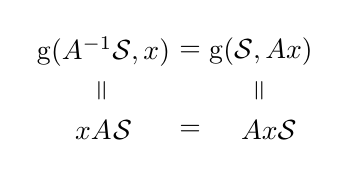
\begin{tikzpicture}
    \node at (0, 0) {$\gauge(A^{-1}\mathcal{S}, x)$};
    \node at (1.1, 0) {$=$};
    \node at (2, 0) {$\gauge(\mathcal{S}, Ax)$};
    \node at (0, -0.5) {$\verteq$};
    \node at (2, -0.5) {$\verteq$};
    \node at (0, -1) {$\supfun{x}{A^{\Tr}\polar{\mathcal{S}}}$};
    \node at (1.1, -1) {$=$};
    \node at (2.1, -1) {$\supfun{Ax}{\polar{\mathcal{S}}}$};
  \end{tikzpicture}
  \caption{Relation between \propref{gaugesupp}, \propref{gA}, \propref{hA} and \propref{podu}.}
  \label{fig:polar_image}
\end{figure}

\propref{podu} plays a prominent role in \chapref{mci}.
The following example provides a geometric intuition for it.

\begin{myexem}
  \label{exem:rockA}
  We can rewrite $(A\Cset)^\circ = A^{-\Tr}(\Cset^\circ)$
  as follows:
  \begin{equation}
    \label{eq:rockAiff}
    x \in (A\Cset)^\circ \iff A^\Tr x \in \Cset^\circ.
  \end{equation}
  Let $\Cset$ be a sphere of radius 1 centered at $(0,0,2)$ and $A$ be the linear projection on the plane $z = 0$.
  With these choices of $\Cset$ and $A$, the set $A\Cset$ is the circle of radius 1 of the plane $z = 0$ centered at the origin.
  This is illustrated by the \figref{rockA}.
  Let $x$ be the normal vector of the line of the plane $z = 0$ shown in \figref{rockA}.
  By \eqref{eq:rockAiff}, $x$ is in the polar of the circle, if and only if
  $A^\Tr x$, which is the plane perpendicular to the plane $z = 0$ containing the line,
  is in the polar of the sphere.
\end{myexem}

\begin{figure}
  \centering
  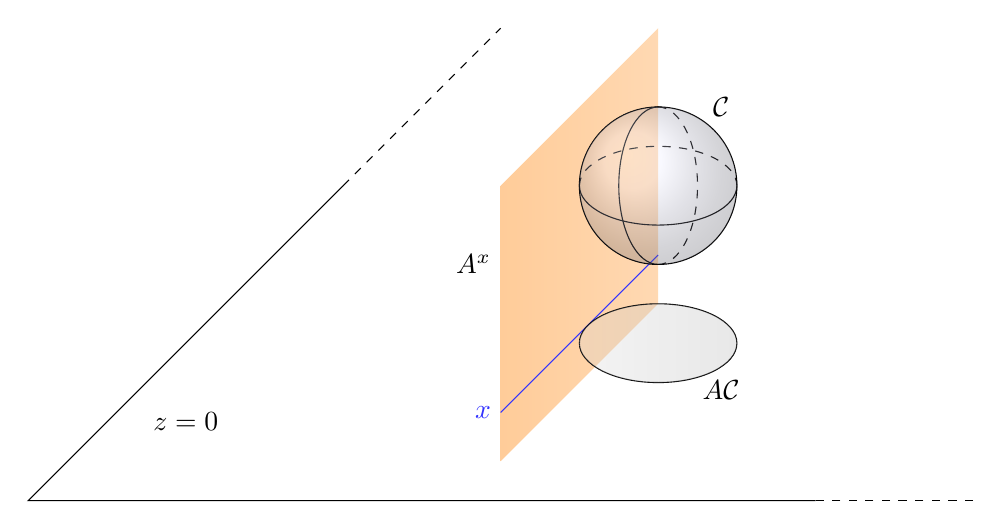
\begin{tikzpicture}
    \shade[left color=orange!40,right color=orange!30] (-2,-1.5) -- (-2,2) -- (0,4) -- (0,.5) -- (-2,-1.5);
    \node[left] at (-2,1) {$A^\Tr x$};

    \draw[blue!80] (-2,-0.88) -- (0,1.12);
    \node[left, blue!80] at (-2,-.88) {$x$};

    \draw (-1,2) arc (180:360:1 and 0.5);
    \draw[dashed] (-1,2) arc (180:0:1 and 0.5);
    \draw (0,3) arc (90:270:0.5 and 1);
    \draw[dashed] (0,3) arc (90:-90:0.5 and 1);
    \draw (0,2) circle (1);
    \shade[ball color=blue!10!white,opacity=0.3] (0,2) circle (1cm);
    \node at (.8,3) {$\Cset$};

    \draw (0,0) ellipse (1 and 0.5);
    \shade[left color=black!15,right color=black!30,opacity=0.3] (0,0) circle (1 and 0.5);
    \node at (.8,-.6) {$A\Cset$};

    \draw[dashed] (4,-2) -- (2,-2);
    \draw (2,-2) -- (-8,-2) -- (-4,2);
    \draw[dashed] (-4,2) -- (-2,4);
    \node at (-6,-1) {$z = 0$};
  \end{tikzpicture}
  \caption{Illustration for \exemref{rockA}.}
  \label{fig:rockA}
\end{figure}

The \emph{barrier cone} of a convex set $\Cset$ is the set of $y$ such that for some $\beta \in \R$, $\la x, y \ra \leq \beta$ for all $x \in \Cset$.
The polar of a set $\Sset$ is
\[ \Sset^\circ = \{\, y \in \R^n \mid \la x, y \ra \leq 1, \forall x \in \Sset \,\}. \]
The polar transformation satisfies the following property:
For any convex sets $\Sset, \Tset$,
\begin{equation}
  \label{eq:revincl}
  \Sset \subseteq \Tset \Leftrightarrow \polar{\Tset} \subseteq \polar{\Sset}.
\end{equation}



\subsection{Polar correspondence of boundary points}

\begin{mydef}[{Tangent cone \cite[Definition~4.6]{blanchini2015set}}]
  Given a closed convex set $\mathcal{S}$ and a distance function $\dist{\mathcal{S}}{x}$,
  the \emph{tangent cone} to $\mathcal{S}$ at $x$ is defined as follows:
  \[ T_{\mathcal{S}}(x) = \left\{\, y \mid \lim_{\tau \to 0} \frac{\dist{\mathcal{S}}{x + \tau y}}{\tau} = 0 \,\right\}. \]
  The tangent cone is a convex cone and is independent of the distance chosen.
\end{mydef}


For a convex set $\Csetvar$, the \emph{normal cone} is the polar of the tangent cone $N_\Csetvar(x) = \polar{T_\Csetvar}(x)$.

\begin{myprop} %
  \label{prop:normal}
  Given a closed convex set $\Csetvar$ containing the origin,
  if $\gauge_p(\Csetvar, x)$ is differentiable at $x \in \partial \Csetvar$ then $N_{\Csetvar}(x) = \{\grad \gauge_p(\Csetvar, x)\}$.
\end{myprop}


The exposed face is also called the support set in \cite[Section~1.7.1]{schneider2013convex}.
\begin{mydef}[{Exposed face \cite[Definition~C.3.1.3]{hiriart2012fundamentals}}]
  Consider a nonempty closed convex set $\Csetvar$.
  Given a vector $y \neq 0$, the \emph{exposed face} of $\Csetvar$ associated
  to $y$ is
  \[
    F_\Csetvar(y) = \setbuild{x \in \Csetvar}{\la x, y \ra = \supfun{y}{\Csetvar}}.
  \]
\end{mydef}


\begin{myprop}[{\cite[Proposition~C.3.1.4]{hiriart2012fundamentals}}]
  \label{prop:normalsupfun}
  Consider a nonempty closed convex set $\Csetvar$.
  For any $x \in \Csetvar$ and nonzero vector $y$,
  $x \in F_\Csetvar(y)$ if and only if $y \in N_\Csetvar(x)$.
\end{myprop}

When the support function is differentiable, $F_\Csetvar$ is a singleton and may be directly obtained from $z$
using the following result:
\begin{myprop}[{\cite[Corollary~25.1.2]{rockafellar2015convex}}]
  \label{prop:exposed}
  Given a nonempty closed convex set $\Csetvar$,
  if $\supfun{y}{\Csetvar}$ is differentiable at $y$ then $F_{\Csetvar}(y) = \{\grad \supfun{y}{\Csetvar}\}$.
\end{myprop}
For nonempty compact convex sets, the differentiability at $y$ is even equivalent to the unicity of $F_{\Csetvar}(y)$~\cite[Corollary~1.7.3]{schneider2013convex}.

A similar flavor of \propref{normalsupfun} in terms of conjugacy is given
by the following:
\begin{myprop}[{\cite[Theorem~23.5]{rockafellar2015convex}}]
  \label{prop:conjpartial}
  For any proper convex function $f$ and vectors $x, y$,
  $y \in \partial f(x)$ if and only if $x \in \partial f^*(y)$.
\end{myprop}

For differentiable functions, this allows to compute the conjugate
of a function by inverting its gradient.
\begin{mycoro}
  \label{coro:conjdiff}
  For any proper convex differentiable function $f$ and vectors $x, y$,
  $y = \grad f(x)$ if and only if $x = \grad f^*(y)$.
\end{mycoro}

\section{Polyhedra and Polytopes}
\label{sec:polyhedra}

Hyperplanes and halfspaces are respectively denoted by
\begin{align*}
  \hyperplane{a}{\alpha} = \{\, x \mid a^\Tr x = \alpha \,\}\\
  \halfspace{a}{\alpha} = \{\, x \mid a^\Tr x \le \alpha \,\}
\end{align*}
For homogeneous hyperplanes and halfspaces, the constant is zero so we simply write $\hhyperplane{a}$ and $\hhalfspace{a}$.
\begin{align*}
  \hhyperplane{a} = \{\, x \mid a^\Tr x = 0 \,\}\\
  \hhalfspace{a} = \{\, x \mid a^\Tr x \ge 0 \,\}
\end{align*}
Note the different sign for the halfspace between $\halfspace{a}{\alpha}$ and $\hhalfspace{a}$.

The intersection of finitely many halfspaces is called a \emph{polyhedral convex set} or a \emph{polyhedron}.
The convex hull of finitely many points is called a \emph{polytope}.

\begin{mytheo}[Weyl-Minkowski]
  \label{theo:weylminkowski}
  Every polytope is a polyhedron. Every bounded polyhedron is a polytope.
\end{mytheo}


\subsection{\hrep{} and \vrep{}}

A halfspace can be seen as a point in the polar set.
\begin{myprop}
  \label{prop:vhpolar}
  Consider a halfspace $\halfspace{a}{\alpha}$ with $\alpha > 0$
  and a closed convex set $\mathcal{S}$ containing the origin.
  The inclusion $\mathcal{S} \subseteq \halfspace{a}{\alpha}$
  is equivalent to $a/\alpha \in \polar{\mathcal{S}}$.
\end{myprop}

\begin{mytheo}[Weyl-Minkowski (continued)]
  \label{theo:weylminkowskicont}
  For a subset $\Pset$ of $\R^n$, the following statements are equivalent
  \begin{itemize}
    \item $\Pset$ has an \emph{\hrep}, that is, there are $\ineqnum$ vectors $a_i \in \R^n$ and $\ineqnum$ scalars $\alpha_i \in \R$ such that
      \begin{equation}
        \label{eq:simpleHrep}
        \Pset = \setbuild{x}{a_i^\Tr x \le \alpha_i, \forall i} = \bigcap_i \halfspace{a_i}{\alpha_i}.
      \end{equation}
    \item $\Pset$ has a \emph{\vrep}, that is, there is finitely many vectors $v_1, \ldots, v_s \in \R^n$, $r_1, \ldots, r_t \in \R^n$ such that
      \begin{equation}
        \label{eq:Vrep}
        \Pset = \conv\{v_1, \ldots, v_s\} + \cone\{r_1, \ldots, r_t\}. %
      \end{equation}
      Or equivalently, there exists matrices $V \in \R^{n \times s}, R \in \R^{n \times t}$ such that
      \begin{equation}
      \label{eq:simpleVrep}
        \Pset = \setbuild{x \in \R^n}{\exists \lambda \in \stdsimplex{s}, \mu \geq 0, x = V\lambda + R\mu}.
      \end{equation}
  \end{itemize}
\end{mytheo}

\begin{mydef}
  The set of \emph{H-representations} of a polyhedron $\Pset \subseteq \R^n$, denoted $\Hrep(\mathcal{P})$ is the family of sets of pairs $(a_i, \alpha_i)_{i=1}^{\ineqnum} \in \R^{n+1}$ such that \eqref{eq:simpleHrep} holds.
\end{mydef}

\begin{mydef}
  The set of \emph{homogeneous H-representations} of a polyhedral cone $\Pset \subseteq \R^n$, denoted $\Hrep(\mathcal{P})$ is the family of sets $(a_i)_{i=1}^{\ineqnum} \in \R^{n}$ such that
  \[ \Pset = \setbuild{x}{a_i^\Tr x \ge 0, \forall i} = \bigcap_i \hhalfspace{a_i}. \]
\end{mydef}

The V-representation of a polytope containing the origin in its interior can directly be
obtained from the H-representation.
\begin{myprop} %
  Consider a polytope $\Pset$ with H-representation given by
  $(a_i, \alpha_i)_{i=1}^{\ineqnum} \in \Hrep(\Pset)$.
  If $\Pset$ contains the origin in its interior then
  $(a_i / \alpha_i)_{i=1}^{\ineqnum} \in \Vrep(\polar{\Pset})$.
\end{myprop}

As a consequence, we can complete \propref{polarnorm} which only gave the polar of
the $p$-norm for $1 < p < \infty$.
\begin{mycoro}
  \label{coro:polar1norm}
  The polar of the unit ball of the 1-norm is the unit ball of the $\infty$-norm.
\end{mycoro}

The H-representation of polyhedron gives the gauge function.


\begin{myprop}
  \label{prop:gaugepolyhedron}
  Consider a polyhedron $\Pset$ with H-representation given by
  $(a_i, \alpha_i)_{i=1}^{\ineqnum} \in \Hrep(\Pset)$.
  If $\Pset$ contains the origin in its interior then
  \begin{equation*}
    \gauge(\Pset, x) = \max_{i=1}^\ineqnum \sprod{a_i / \alpha_i}{x}.
  \end{equation*}
  \begin{proof}
    As the origin is in the interior of $\Pset$,
    $\alpha_i > 0$ for $i = 1, \ldots, \ineqnum$.
    Therefore, $\gauge(\halfspace{a_i}{\alpha_i}, x) = \sprod{a_i / \alpha_i}{x}$.
    By \theoref{weylminkowskicont}, $\Pset$ is the intersection of the hyperplanes, see \eqref{eq:simpleHrep}.
    The result follows from \propref{gaugeint}.
  \end{proof}
\end{myprop}

As a consequence, the following propositions follow from \propref{gaugeint} and \propref{gA}.
\begin{myprop}
  Consider polyhedra $\Pset_1, \Pset_2$, the concatenation
  of a H-representation for each set
  is a H-representation for their intersection
  $\Pset_1 \cap \Pset_2$.
\end{myprop}
\begin{myprop}
  \label{prop:gApolyhedron}
  Consider a polyhedron $\Pset$ with H-representation given by
  $(a_i, \alpha_i)_{i=1}^{\ineqnum} \in \Hrep(\Pset)$ and
  a matrix $A \in \R^{n \times m}$.
  A H-representation of the preimage of $A^{-1}\Pset$ is given by
  \begin{equation*}
    (A^\Tr a_i, \alpha_i)_{i=1}^{\ineqnum} \in \Hrep(A^{-1}\Pset).
  \end{equation*}
\end{myprop}

\begin{mydef}
  The set of \emph{V-representations} of a polyhedral cone $\Pset \subseteq \R^n$,
  denoted $\Hrep(\mathcal{P})$ is the family of sets of
  vectors $v_1, \ldots, v_s \in \R^n$, $r_1, \ldots, r_t \in \R^n$
  such that \eqref{eq:Vrep} holds.
\end{mydef}

By \propref{gaugesupp} and \propref{vhpolar},
the following proposition follows from \propref{gaugepolyhedron}.

\begin{myprop}
  \label{prop:supfunvrep}
  Consider a nonempty polyhedron $\Pset$ with V-representation given by
  $v_1, \ldots, v_s \in \R^n$, $r_1, \ldots, r_t \in \R^n$.
  The support function of $\Pset$ is given by
  \begin{equation*}
    \supfun{x}{\Pset} =
    \begin{cases}
      \infty & \text{ if } \exists i \in [t]: \la r_i, x \ra > 0,\\
      \max_{i=1}^s \la v_i, x \ra & \text{ otherwise}.
    \end{cases}
  \end{equation*}
\end{myprop}


As a consequence of \propref{supfunvrep}, the following propositions follow from \propref{supportsum} and \propref{hA}.
\begin{myprop}
  \label{prop:polysum}
  Consider polyhedra $\Pset_1, \Pset_2$, with V-representations
  $v_1^k, \ldots, v_{s_k}^k \in \R^n$, $r_1^k, \ldots, r_{t_k}^k \in \R^n$ for $\Pset_k$.
  The pairwise sum of the vertices $v_i^1 + v_j^2$ for $i \in s_1, j \in s_2$
  and concatenation of the rays form a V-representation
  for the Minkowski sum $\Pset_1 + \Pset_2$.
  \begin{proof}
    It follows from \propref{supportsum}, noticing that
    \[
      \max_{i=1}^{s_1} \la v_i^1, x \ra + \max_{i=1}^{s_2} \la v_i^2, x \ra
      = \max_{i=1}^{s_1} \max_{j=1}^{s_2} \la v_i^1 + v_j^2, x \ra.
    \]
  \end{proof}
\end{myprop}
The quadratic increase of the number of vertices of the V-representation
is resolved by the Z-representation used by Zonotopes, see \secref{zonotope}.

\begin{myprop}
  \label{prop:hApolyhedron}
  Consider a polyhedron $\Pset$ with V-representation given by
  $((v_i)_{i=1}^s, (r_i)_{i=1}^t) \in \Vrep(\Pset)$
  and a matrix $A \in \R^{m \times n}$.
  A V-representation of the image $A\Pset$ is given by
  \begin{equation*}
    ((Av_i)_{i=1}^s, (Ar_i)_{i=1}^t) \in \Vrep(A\Pset).
  \end{equation*}
\end{myprop}

Similarly to \cororef{supproj}, we have the following corollary.
\begin{mycoro}
  \label{coro:polyproj}
  Consider a polyhedron $\Pset$ with V-representation given by
  $((v_i)_{i=1}^s, (r_i)_{i=1}^t) \in \Vrep(\Pset)$
  and a subset $I \subseteq [n]$.
  A V-representation of the projection of $\Pset$ on $I$ is given by
  \begin{equation*}
    ((\pi_{I, n}v_i)_{i=1}^s, (\pi_{I, n}r_i)_{i=1}^t) \in \Vrep(\pi_{I, n}(\Pset)).
  \end{equation*}
\end{mycoro}

For a polyhedral cone, the representations can be simplified:
\begin{itemize}
  \item the \hrep{} is
    \begin{equation}
      \label{eq:coneHrep}
      \Pset = \setbuild{x \in \R^n}{Ax \geq 0}.
    \end{equation}
  \item and the \emph{\rrep} is
    \begin{equation}
      \label{eq:coneVrep}
      \Pset = \{\, x \in \R^n \mid \exists \lambda \geq 0, x = R\lambda \,\}.
    \end{equation}
\end{itemize}

Every convex set $\Cset \in \R^n$ can be regarded as the cross-section of a convex cone $\Kset \in \R^{n+1}$.
Indeed, let $\Kset = \cone\{\, (1,x) \mid x \in \Cset \,\}$,
the set $\Cset$ is the intersection of $\Kset$ with the hyperplane $\{\, (\lambda,x) \mid \lambda = 1\,\}$.

Let $A^c, R^c$ be the matrices $A$ and $R$ of the \hrep{} and \rrep{} of $\Kset$.
We have
\begin{align*}
  A^c & = \begin{bmatrix}-b & A\end{bmatrix}\\
  R^c & = \begin{bmatrix}\1^\Tr & 0\\V & R\end{bmatrix}\\
  b & = -A^c_{:,1}\\
  A & = A^c_{:,2:}.
\end{align*}
To extract $V$ and $R$ from $R^c$ we need to scale the columns of $R_c$ by nonnegative scalars so that the first row contains only zeros and ones (we drop the columns containing negative numbers in the first row).
Then the columns with one in the first row are put in $V$ and the columns with zeros in the first row are put in $R$.

The pair $(A, R)$ is called a Double Description (DD)-pair.
The DD-pair of the dual cone is $(R^\Tr, A^\Tr)$.
\begin{align}
  \label{eq:coneHrepdual}
  \Pset^* & = \{\, x \in \R^n \mid R^\Tr x \geq 0 \,\}\\
  \label{eq:coneVrepdual}
  \Pset^* & = \{\, x \in \R^n \mid \exists \lambda \geq 0, x = A^\Tr\lambda \,\}.
\end{align}

This shows that going from $A$ to $R$, which is called the \emph{vertex enumeration} problem, or going from $R$ to $A$, which is called the \emph{convex hull} problem, are essentially the same problems: the \emph{representation conversion} problem.

One way to compute $A$ from $R$ is to eliminate $\lambda$ from the linear system of \eqref{eq:coneVrep}.
To compute $R$ from $A$ we can do the same to \eqref{eq:coneVrepdual}.
Eliminating variables from a polyhedron is called \emph{polyhedral projection}.
That is, we have just provided a polynomial reduction of representation conversion to polyhedral projection of \hrep{}.

The family of polyhedra has the important property of being closed under projection:
\begin{mytheo}[Fourier-Motzkin]
  \label{theo:fourier_motzkin}
  The projection of a polyhedral set on a linear subspace is a polyhedral set.
\end{mytheo}
This is proved constructively by exhibiting the Fourier-Motzkin elimination
which,
given the H-representation of a polyhedron,
provides a procedure to compute the H-representation of the polyhedron obtained by eliminating one coordinate.
Even if there exists heuristics to limit this, the Fourier-Motzkin elimination procedure
generally generates a redundant H-representation.
Removing these redundant halfspaces is crucial when eliminating several coordinates
to avoid a prohibitive number of redundant halfspaces.

Polyhedral projection of a polyhedron in its \vrep{} is simple.
As shown by \cororef{polyproj}, it boils down to dropping the eliminated coordinates of vertices and rays.
We can see that polyhedral projection of an \hrep{} can be achieved by two representation conversion and the polyhedral projection of \vrep{}.
This provides a polynomial reduction of polyhedral projection of \hrep{} to representation conversion.

This shows that representation conversion is essentially ``as hard'' as polyhedral projection.

\subsection{Containment and inclusion}

Given a point $x$, its containment in a polyhedron can be checked using either of the following two properties.
\begin{myprop}
  \label{prop:vinhrep}
  A point $x$ belongs to a polyhedron $\Pset$ defined by \eqref{eq:simpleHrep} if and only if
  $\la a_i, x \ra \le \alpha_i$ for $i = 1, \ldots, \ineqnum$.
\end{myprop}
\begin{myprop}
  \label{prop:vinvrep}
  A point $x$ belongs to a polyhedron $\Pset$ defined by \eqref{eq:simpleVrep} if and only if there exists $(\lambda_1 \ldots, \lambda_s) \in \stdsimplex{s}$ and
  $\gamma_1, \ldots, \gamma_t \in \R_+$ such that
  \[ x = \sum_{i=1}^s \lambda_i v_i + \sum_{i=1}^t \gamma_i r_i. \]
\end{myprop}

Given a ray $\ray(r)$, its inclusion in a polyhedron can be checked using either of the following two properties.
\begin{myprop}
  \label{prop:rinhrep}
  There exists a translation of the ray $\ray{r}$ that is included in a polyhedron $\Pset$ defined by \eqref{eq:simpleHrep} if and only if
  $\la a_i, r \ra \le 0$ for $i = 1, \ldots, \ineqnum$.
\end{myprop}
\begin{myprop}
  \label{prop:rinvrep}
  There exists a translation of the ray $\ray{r}$ that is included in a polyhedron $\Pset$ defined by \eqref{eq:Vrep} if and only if there exists
  $\gamma_1, \ldots, \gamma_t \in \R_+$ such that
  \[ r = \sum_{i=1}^t \gamma_i r_i. \]
\end{myprop}

Given a halfspace $\halfspace{a}{\alpha}$, the inclusion of a polyhedron in the halfspace can be checked using either of the following two properties.
\begin{myprop}
  \label{prop:hinvrep}
  A polyhedron $\Pset$ defined by \eqref{eq:simpleVrep} is included in a halfspace $\halfspace{a}{\alpha}$ if and only if
  $\la a, v_i \ra \le \alpha$ for $i = 1, \ldots, s$,
  $\la a, r_i \ra \le 0$ for $i = 1, \ldots, t$
  and either $s > 0$ or $t = 0$ or $\alpha \ge 0$.
\end{myprop}
\begin{myprop}
  \label{prop:hinhrep}
  A polyhedron $\Pset$ defined by \eqref{eq:simpleHrep} is included in a halfspace $\halfspace{a}{\alpha}$ if and only if there exists $(\lambda_1 \ldots, \lambda_\ineqnum) \in \R_+$ such that
  \[ \alpha \ge \sum_{i=1}^\ineqnum \lambda_i \alpha_i \]
  and
  \[ a = \sum_{i=1}^\ineqnum \lambda_i a_i. \]
\end{myprop}
The \propref{hinhrep} can be seen as a quadratic module (see \defref{qmodule}) certificate of nonnegativity of
the affine polynomial $\alpha - \la a, x \ra$ over the polyhedron $\Pset$.

\subsubsection{Affine hull}
\label{sec:affine_hull}
In this section, we analyse the following questions:
1) Given the H-representation, how to determine the affine hull ?
2) Let the \emph{line hull} of a polyhedron be the set of lines contained
in the polyhedron.
The corresponding question for the V-representation is how to determine the line hull given the V-representation.

A first important fact to highlight is that the coordinates of the hyperplanes
defining the affine hull (resp. lines defining the line hull)
are among the halfspaces (resp. rays) of any H-representation (resp. V-representation) of the polyhedron.
It remains to determine this subset $I$ or halfspaces or rays.
One simple approach, which is not the most efficient computationally,
is to check for each $i \in [\ineqnum]$ (resp $i \in [t]$) whether
$\Pset \subseteq \halfspace{-a_i}{-\alpha_i}$ (resp $\ray(-r_i) \subseteq \Pset$)
with \propref{hinhrep} (resp. \propref{rinvrep}).
This approach requires the solution of one linear program per halfspace
(resp. ray).
In fact, it turns out that a more sophisticated approach allows to only
solve a number of linear programs that is bounded by the dimension of the space.

\begin{myprog}[Primal-dual pair of programs for detecting lines]
  \label{prog:line}
  \begin{align*}
    \maxi_{x, z} z && \mini_{\lambda} 0\\
    \la r_i, x \ra & \ge z & \lambda & \ge 0\\
    x & \text{ free} & \sum_{i=1}^t r_i \lambda_i & = 0\\
    z & \text{ free} & \sum_{i=1}^t \lambda_i & = 1.
  \end{align*}
\end{myprog}

\begin{myprop}
  \label{prop:linesubset}
  Consider a polyhedron $\Pset$ with V-representation given by
  $((v_i)_{i=1}^s, (r_i)_{i=1}^t) \in \Vrep(\Pset)$.
  Let $\opt{x}, \opt{z}, \opt{\lambda}$ be the optimal solution of \progref{line}.

  The polyhedron contains a line if and only if $\opt{z} = 0$.
  Moreover, there exists a subset $I \subseteq [t]$ such that
  the line hull of $\Pset$ is generated by $r_i$ for $i \in I$.
  Furthermore, we have the following properties:
  \begin{enumerate}
    \item
      \label{enum:dual_line}
      If $\opt{\lambda}_i > 0$ then $i \in I$.
    \item
      \label{enum:primal_line}
      If $\la r_i, \opt{x} \ra > z$ then $i \notin I$.
  \end{enumerate}

  \begin{proof}
    By \propref{rinvrep}, if there is a line generated by $l$ included in the polyhedron
    then there exists $\mu_i \ge 0$ and $\nu_i \ge 0$ such that
    $\sum_i \mu_i r_i = l$ and $\sum_i \nu_i r_i = -l$.
    We deduce from this that $\sum \lambda_i r_i = 0$ where $\lambda = \mu + \nu$.

    Conversely, if there are $\lambda \ge 0$ such that $\sum \lambda_i r_i = 0$ then let
    $j$ be such that $\lambda_j > 0$.
    We have $\sum_{i \neq j} \lambda_i/\lambda_j r_i = -r_j$.
    As both $r_j$ and $-r_j$ are in the cone,
    $r_j$ generates a line in the cone.
    However, this means that we now have $\sum_{i \neq j} \lambda_i/\lambda_j r_i \equiv 0 \pmod{r_j}$ so if there is another $\lambda_i$
    with nonzero value, we can transform it to a line as well.
    Therefore, we have a line generated by $r_i$ for each $i$ such that $\lambda_i > 0$.

    If $\opt{z} = 0$, as $\la r_i, \opt{x} \ra \ge 0$ for each $i$,
    any ray $r$ in the cone is such that $\la r, \opt{x} \ra \ge 0$.
    Therefore, if $\la r_i, x \ra > z$ for some $i$,
    we know that $\ray(-r_i)$ does not belong to the cone.
    That is, $i \notin I$.
  \end{proof}
\end{myprop}

\begin{myprog}[Primal-dual pair of programs for detecting hyperplanes]
  \label{prog:aff}
  \begin{align*}
    \maxi_{x, z} z && \mini_{\lambda} \sum \lambda_i \alpha_i\\
    \la a_i, x \ra & \ge \alpha_i + z & \lambda & \ge 0\\
    x & \text{ free} & \sum_{i=1}^\ineqnum a_i \lambda_i & = 0\\
    z & \text{ free} & \sum_{i=1}^\ineqnum \lambda_i & = 1.
  \end{align*}
\end{myprog}

\begin{myprop}
  \label{prop:affsubset}
  Consider a polyhedron $\Pset$ with H-representation given by
  $(a_i, \alpha_i)_{i=1}^{\ineqnum} \in \Hrep(\Pset)$.
  Let $\opt{x}, \opt{z}, \opt{\lambda}$ be the optimal solution of \progref{line}.

  The polyhedron is included in a hyperplane if and only if $\opt{z} \le 0$.
  Moreover, there exists a subset $I \subseteq [\ineqnum]$ such that
  \[ \aff(\Pset) = \cap_{i \in I} \hyperplane{a_i}{\alpha_i}. \]
  Furthermore, we have the following properties:
  \begin{enumerate} %
    \item
      \label{enum:dual_aff}
      If $\opt{\lambda}_i > 0$ then $i \in I$.
    \item
      \label{enum:primal_aff}
      If $\la a_i, \opt{x} \ra > \alpha_i + z$ then $i \notin I$.
    \item
      \label{enum:empty_aff}
      If $\opt{z} < 0$, then the polyhedron is empty.
  \end{enumerate}
  \begin{proof}
    By \propref{hinhrep}, if the polyhedron is included in a hyperplane $\hyperplane{b}{\beta}$
    then there exists $\mu_i \ge 0$ and $\nu_i \ge 0$ such that
    $\sum_i \mu_i a_i = b$, $\sum_i \mu_i \alpha_i \le \beta$, $\sum_i \nu_i a_i = -b$ and $\sum_i \mu_i \alpha_i \le -\beta$.
    We deduce from this that $\sum \lambda_i a_i = 0$ and $\sum_i \lambda_i \alpha_i \le 0$ where $\lambda = \mu + \nu$.

    Conversely, if there are $\lambda \ge 0$ such that $\sum \lambda_i a_i = 0$ and $\sum \lambda \alpha_i \le 0$ then let
    $j$ be such that $\lambda_j > 0$.
    We have $\sum_{i \neq j} \lambda_i/\lambda_j a_i = -a_j$ and $\sum_{i \neq j} \lambda_i/\lambda_j \alpha_i \le -\alpha_j$.
    As the polyhedron is included in both $\halfspace{a_j}{\alpha_j}$ and $\halfspace{-a_j}{-\alpha_j}$,
    it is included in $\hyperplane{a_j}{\alpha_j}$.
    However, this means that we now have $\sum_{i \neq j} \lambda_i/\lambda_j (\la a_i, x \ra + \alpha_i) \equiv \la 0, x \ra + \beta \pmod{\la a_j, x \ra + \alpha_j}$ where $\beta \le 0$ so if there is another $\lambda_i$
    with nonzero value, we can transform it to a hyperplane as well.
    Therefore, we have a hyperplane $\hyperplane{a_i}{\alpha_i}$ for each $i$ such that $\lambda_i > 0$.

    If $\opt{z} = 0$, as $\la a_i, \opt{x} \ra \ge \alpha_i$ for each $i$,
    any halfspace $\halfspace{b}{\beta}$ that the polyhedron is included in is such that $\la b, \opt{x} \ra \ge \beta$.
    Therefore, if $\la a_i, x \ra > \alpha_i$ for some $i$,
    we know that $\halfspace{-a_i}{-\alpha_i}$ does not belong to the cone.
    That is, $i \notin I$.
  \end{proof}
\end{myprop}

\begin{myrem}
  \label{rem:cddlibaff}
  In the latest version of cddlib~\cite{fukuda2003cdd} at the time of writing (v0.94j),
  \texttt{dd\_MatrixCanonicalizeLinearity} calls
  \texttt{dd\_ImplicitLinearityRows} and \texttt{dd\_ImplicitLinearityRows}
  solves the \progref{line} for V-representation and \progref{aff}
  for H-representation.
  Then, using \propref{linesubset}.\ref{enum:primal_line} (resp. \propref{affsubset}.\ref{enum:primal_aff}),
  some rays (resp. halfspaces) are determined not to correspond to a linearity.
  For all other ray $r_i$ (resp. halfspace $\halfspace{a_i}{\alpha_i}$), it calls
  \texttt{dd\_ImplicitLinearity} which solves an LP
  to determine whether $-r_i$ is included in the cone with \propref{rinvrep} (resp. the polyhedron is included in $-\halfspace{a_i}{-\alpha_i}$ with \propref{hinhrep}).
  The number of linear programs to solve in the worstcase is equal to the number of rays (resp. halfspaces).

  By comparison, \progref{line} (resp. \progref{aff}) allows to find all implicit linearities with a number of linear program equal to the dimension of the space in the worst case.
  This is significantly more efficient as the number of rays (resp. halfspaces) can be exponential
  in terms of the dimension of the space.
  Indeed, everytime \progref{line} (resp. \progref{aff}) is solved,
  either no now linearity is to be detected or,
  \propref{linesubset}.\ref{enum:dual_line}/\propref{affsubset}.\ref{enum:dual_aff}
  allows to increase the dimension of the line hull (resp. affine hull)
  by at least one.
  As the dimension is upper bounded by the dimension of the space, the number of
  LPs to solve is also upper bounded by the dimension of the space.
  This is the procedure implemented in \jlpkg{Polyhedra}.
\end{myrem}

\subsection{Output-sensitive computational complexity}
The complexity of algorithms is commonly described using only the input size (in bits) and not the output size.
This is not appropriate for representation conversion and polyhedral projection algorithms that need to list the facets (resp. vertices, rays) of a polyhedron.
Indeed, the output size itself might not be polynomial in terms of the input size.
We say that an algorithm is \emph{output-sensitive} if it is in P-TIME in both the input and output size.
It was shown that none of the known algorithms for the representation conversion are output-sensitive~\cite{avis1995good} but
it is still unknown whether there exists an output-sensitive algorithm for this problem.

An algorithm with a large output might produce its output incrementally without needing to store its output to continue.
Therefore it might run in P-SPACE in its input size even if its output size is exponential in its input size.
Such algorithm is said to be \emph{compact} \cite{fukuda1996note}.
This is the case of the reversed search vertex enumeration algorithm implemented in LRS~\cite{avis2000revised}.



\subsection{Zonotopes}
\label{sec:zonotope}

We saw in \propref{polysum} that taking the Minkowski sum of two polytopes
increase the size of the V-representation quadratically (even if some vertices may be redundant).
One way to go around this issue is to define the following representation.
\begin{mydef}
  A set of vectors $c, (v_i)_{i=1}^z$ is a \emph{Z-representation}
  of a polyhedron $\Pset$,
  denoted $(c, (v_i)_{i=1}^z) \in \Zrep(\Pset)$,
  if
  \[
    \Pset = \{c\} + \sum_{i=1}^z \conv(-v_i, v_i).
  \]
\end{mydef}
Note that not all polytopes have a Z-representation.
The polytopes with a Z-representation are called Zonotopes.

\begin{myprop}
  Consider a nonempty zonotope $\Pset$ with Z-representation given by
  $(c, (v_i)_{i=1}^z) \in \Zrep(\Pset)$.
  The support function of $\Pset$ is given by
  \begin{equation*}
    \supfun{x}{\Pset} =
    \la c, x \ra + \sum_{i=1}^z |\la z_i, x \ra|.
  \end{equation*}
\end{myprop}

As a consequence, the following propositions follow from \propref{supportsum} and \propref{hA}.
\begin{myprop}
  \label{prop:zonosum}
  Consider zonotopes $\Pset_1, \Pset_2$, with Z-representations
  $(c^k, (v_i^k)_{i=1}^z) \in \Zrep(\Pset_k)$.
  The tuple made of $c^1 + c^2$
  and the concatenation of $v^1$ and $v^2$
  is a Z-representation for the Minkowski sum $\Pset_1 + \Pset_2$.
\end{myprop}

\begin{myprop}
  Consider a zonotope $\Pset$ with Z-representation given by
  $(c, (v_i)_{i=1}^z) \in \Zrep(\Pset)$
  and a matrix $A \in \R^{m \times n}$.
  A Z-representation of the image $A\Pset$ is given by
  \begin{equation*}
    (Ac, (Av_i)_{i=1}^z) \in \Zrep(A\Pset).
  \end{equation*}
\end{myprop}

We see with these proposition that the zonotope family is closed under
Minkowski sum and image (hence also projection).
However, it is not closed under intersection or convex hull (otherwise any polytope would be a zonotope).



\section{Ellipsoids}
\label{sec:ell}

An \emph{ellipsoid} is defined by
\begin{equation}
  \label{eq:ell}
  \mathcal{E}_P = \setbuild{x \in \R^n}{x^\Tr P x \leq 1}.
\end{equation}
where $P$ is a positive definite matrix.
When $P$ is only positive semidefinite, the set is a \emph{semi-ellipsoid}.

The gauge function and gauge-like function of degree 2 of the ellipsoid are
\begin{align}
  \label{eq:gaugeell}
  \gauge(\mathcal{E}_P, x) & = \sqrt{x^\Tr P x} &
  \gauge_2(\mathcal{E}_P, x) & = x^\Tr P x / 2.
\end{align}

To obtain the polar of $\mathcal{E}_P$, we first develop the following
property of the conjugate of quadratic forms.
\begin{myprop}
  \label{prop:conjquad}
  Given a positive definite matrix $P \in \Pd$, the conjugate of the convex function
  $f(x) = x^\Tr P x / 2$ is the convex function $f^*(y) = y^\Tr P^{-1} y / 2$.
  \begin{proof}
    By \cororef{conjdiff}, $y = Px$ if and only if $x = \grad f^*(y)$.
    Therefore, $\grad f^*(y) = P^{-1}y$ and $f^*(y) = y^\Tr P^{-1} y / 2$.
  \end{proof}
\end{myprop}

We can deduce the following.
\begin{myprop}
  \label{prop:polarell}
  Given a positive definite matrix $P \in \Pd$, the polar of the ellipsoid $\mathcal{E}_P$
  is $\polar{\mathcal{E}}_P = \mathcal{E}_{P^{-1}}$.
  \begin{proof}
    Using \eqref{eq:gaugeell}, \propref{gauge-like} and \propref{conjquad},
    we see that the polar of the gauge function is
    $\gauge(\polar{\mathcal{E}}_P, x) = \polar{\gauge}(\mathcal{E}_P, x) = \sqrt{x^\Tr P^{-1} x}$.
  \end{proof}
\end{myprop}

We deduce the following from \propref{polarell} and \propref{gaugesupp}.
\begin{myprop}
  \label{prop:supfunell}
  Given a positive definite matrix $P \in \Pd$, the support function of the ellipsoid $\mathcal{E}_P$ is $\supfun{y}{\mathcal{E}_P} = \sqrt{y^\Tr P^{-1} y}$.
\end{myprop}

\subsection{Operations}

As the family of ellipsoids is invariant under polarity operation, the
six operations can be considered by pairs $(\cap, \conv \cup)$, $(+, \invsum)$ and $(A, A^{-1})$.
The family of ellipsoids is either invariant under both operations of the pair or none.

The intersection and convex hull of the union of ellipsoid is not necessarily
an ellipsoid, but it is always a \emph{piecewise ellipsoid}, that we study in \secref{pieceell}.

The sum and inverse sum of ellipsoids is not ellipsoidal in general.
By \propref{supportsum} and \propref{supfunell}, we have that
\[ \supfun{y}{\mathcal{E}_{P_1} + \mathcal{E}_{P_2}} = \sqrt{y^\Tr P_1 y} + \sqrt{y^\Tr P_2 y} \]
which is not a quadratic form in general.
The following example provides a simple counterexample of the invariant of the family of ellipsoids under sum and inverse sum.
\begin{myexem}
  Consider the semi-ellipsoids $\mathcal{E}_{e_1e_1^\Tr}$ and $\mathcal{E}_{e_2e_2^\Tr}$.
  By \propref{gaugeinvsum} and \eqref{eq:gaugeell}, we have
  \[
    \gauge(\mathcal{E}_{e_1e_1^\Tr} \invsum \mathcal{E}_{e_2e_2^\Tr}, x)
    = \sqrt{x^\Tr e_1e_1^\Tr x} + \sqrt{x^\Tr e_2e_2^\Tr x}
    = |x_1| + |x_2|.
  \]
  Hence $\mathcal{E}_{e_1e_1^\Tr} \invsum \mathcal{E}_{e_2e_2^\Tr}$ is the unit ball
  of the 1-norm and, by \cororef{polar1norm}, its polar is the $\infty$-norm.
\end{myexem}

We have the following property for the linear preimage of an ellipsoid.
\begin{myprop}
  \label{prop:ellpreimage}
  Given an ellipsoid $\mathcal{E}_P \subseteq \R^n$ and
  a matrix $A \in \R^{n \times m}$, the following holds:
  \[ A^{-1}\mathcal{E}_P = \mathcal{E}_{A^{\Tr}PA}. \]
  \begin{proof}
    This is a consequence of \eqref{eq:gaugeell} and \propref{gA}.
  \end{proof}
\end{myprop}

In view of \propref{supfunell} and \propref{hA},
the linear image of an ellipsoid is more naturally obtained from $P^{-1}$ and its polar.
\begin{myprop}
  \label{prop:ellimage}
  Given an ellipsoid $\mathcal{E}_{P} \subseteq \R^n$ and
  a matrix $A \in \R^{m \times n}$, the following holds:
  \begin{align}
    \label{eq:supfunellimage}
    \supfun{y}{A\mathcal{E}_{P}} & = y^\Tr AP^{-1}A^{\Tr} y\\
    \label{eq:ellimagepolar}
    \polar{A\mathcal{E}_{P}} & = \mathcal{E}_{AP^{-1}A^{\Tr}}.
  \end{align}
  Moreover, if $AP^{-1}A^{\Tr}$ is invertible, we have
  \begin{equation}
    \label{eq:ellimage}
    A\mathcal{E}_{P} = \mathcal{E}_{(AP^{-1}A^{\Tr})^{-1}}.
  \end{equation}
  \begin{proof}
    The equation~\eqref{eq:supfunellimage} follows from \propref{supfunell}
    and \propref{hA}.
    By \propref{gaugesupp} and \propref{supfunell}, equation~\eqref{eq:ellimagepolar}
    is obtained from \eqref{eq:supfunellimage}.
    The set $\mathcal{E}_{AP^{-1}A^{\Tr}}$ is a semi-ellipsoid but it is
    an ellipsoid only if $AP^{-1}A^{\Tr}$ is invertible.
    If it is an ellipsoid, \eqref{eq:ellimage} follows from \propref{polarell} and \eqref{eq:ellimagepolar}.
  \end{proof}
\end{myprop}

\subsection{Boundary points}

The following follows from \eqref{eq:gaugeell} and \propref{normal}.
\begin{myprop}
  \label{prop:normalell}
  Given a positive definite matrix $P \in \Pd$, the normal cone of a vector $x \in \partial \mathcal{E}_P$ is given by
  \(
    N_{\mathcal{E}_P}(x) = \ray(\{Px\}).
  \)
\end{myprop}

The following follows from \propref{supfunell} and \propref{exposed}.
\begin{myprop}
  \label{prop:exposedell}
  Given a positive definite matrix $P \in \Pd$, the exposed face of a vector $y$ is given by
  \(
    F_{\mathcal{E}_P}(y) = \{P^{-1}y\}.
  \)
\end{myprop}

\subsection{Containment and inclusion}

As a consequence of \propref{gaugelikeincl} and \eqref{eq:gaugeell},
the inclusion between ellipsoids is verified using the following property.
\begin{myprop}
  \label{prop:ellincl}
  Consider two ellipsoids $\mathcal{E}_{P_1}, \mathcal{E}_{P_2}$.
  The inclusion $\mathcal{E}_{P_1} \subseteq \mathcal{E}_{P_2}$ is equivalent to
  $P_1 \succeq P_2$.
\end{myprop}

By definition of the gauge function and \propref{schurcomp}, we have
the following two conditions for the containment of a point in an ellipsoid.
\begin{myprop}
  \label{prop:vinell}
  Given a point $x \in \R^n$ and an ellipsoid $\mathcal{E}_P$,
  the membership $x \in \mathcal{E}_P$ is equivalent to the following three equivalent conditions
  \begin{align}
    \label{eq:vinell1}
    x^\Tr P x & \le 1,\\
    \label{eq:vinell2}
    \begin{bmatrix}
      1 & x^\Tr\\
      x & P^{-1}
    \end{bmatrix}
    & \succeq 0,\\
    \label{eq:vinell3}
    P^{-1} & \succeq xx^\Tr.
  \end{align}
  \begin{proof}
    The condition \eqref{eq:vinell1} is by definition of the ellipsoid, see \eqref{eq:ell}.
    The condition \eqref{eq:vinell2} follows from \eqref{eq:vinell1} and \propref{schurcomp}.
    The condition \eqref{eq:vinell3} follows from \eqref{eq:vinell2} and \propref{schurcomp} but we provide here an alternative proof
    that gives a more geometric interpretation.
    As $\mathcal{E}_P$ is a symmetric convex set, $x \in \mathcal{E}_P$
    if and only if $\conv(\{-x, x\}) \subseteq \mathcal{E}_P$.
    By \propref{supfunvrep}, we have $\supfun{y}{\conv(\{-x, x\})} = |\la x, y \ra| = \sqrt{y^\Tr x x^\Tr y}$.
    By \propref{supfunell}, $\supfun{y}{\mathcal{E}_P} = \sqrt{x^\Tr P^{-1} x}$,
    Therefore, by \propref{supportincl}, we have \eqref{eq:vinell3}.
  \end{proof}
\end{myprop}

By \propref{polarell} and \propref{schurcomp}, we have
the following two conditions for the inclusion of an ellipsoid
in a halfspace.
\begin{myprop}
  \label{prop:ellinh}
  Given a halfspace $\halfspace{a}{\alpha} \subseteq \R^n$ with $\alpha > 0$ and an ellipsoid $\mathcal{E}_P$,
  the inclusion $\mathcal{E}_P \subseteq \halfspace{a}{\alpha}$ is equivalent to the following three equivalent conditions
  \begin{align}
    \label{eq:ellinh1}
    a^\Tr P^{-1} a & \le \alpha^2,\\
    \label{eq:ellinh2}
    \begin{bmatrix}
      \alpha^2 & a^\Tr\\
      a & P
    \end{bmatrix}
    & \succeq 0,\\
    \label{eq:ellinh3}
    P & \succeq \alpha^{-2} aa^\Tr.
  \end{align}
  \begin{proof}
    The condition~\eqref{eq:ellinh1} follows \propref{vhpolar} and \propref{polarell}.
    The condition \eqref{eq:ellinh2} follows from \eqref{eq:ellinh1} and \propref{schurcomp}.
    The condition \eqref{eq:ellinh3} follows from \eqref{eq:ellinh2} and \propref{schurcomp} but we provide here an alternative proof
    that gives a more geometric interpretation.
    As $\mathcal{E}_P$ is a symmetric convex set, $\mathcal{E}_P \subseteq \halfspace{a}{\alpha}$
    if and only if $\mathcal{E}_P \subseteq \halfspace{a}{\alpha} \cap \halfspace{-a}{\alpha}$.
    By \propref{gaugepolyhedron}, we have $\gauge(\halfspace{a}{\alpha} \cap \halfspace{-a}{\alpha}, x) = |\la x, a/\alpha \ra| = \sqrt{x^\Tr a a^\Tr x} / \alpha$.
    By \propref{supfunell}, $\supfun{y}{\mathcal{E}_P} = \sqrt{x^\Tr P^{-1} x}$,
    Therefore, by \eqref{eq:gaugeell} and \propref{gaugeincl}, we have \eqref{eq:ellinh3}.
  \end{proof}
\end{myprop}

\subsection{Volume and semi-axis}

An ellipsoid $\mathcal{E}_P$ can be represented as the rotation of
an ellipsoid of the form $\mathcal{E}_{e_1e_1^\Tr / a_1^2 + \ldots + e_ne_n^\Tr / a_n^2}$.
Geometrically, the numbers $a_i$ represent the length of the semi-axis of the ellipsoid.
The length of the semi-axes is an invariant of the ellipsoids under rotation.

The volume of an ellipsoid does not depend on the rotation
and can be expressed in terms of this invariant.
\begin{myprop}
  The volume of an ellipsoid with semi-axis of length
  $a_1, \ldots, a_n$ is given by
  \[ \frac{\pi^{n/2}}{\Gamma(n/2 + 1)} \prod_{i=1}^n a_i. \]
\end{myprop}

The numbers $a_i$ are the inverse of square root of the eigenvalues of the matrix $P$,
in other words, they are the square root of the eigenvalues
of the inverse of $P$.
The following two properties follow from this observation.

\begin{myprop}
  \label{prop:detell}
  The volume of an ellipsoid $\mathcal{E}_P$ is given by
  \[ \frac{\pi^{n/2}}{\Gamma(n/2 + 1) \sqrt{\det(P)}}. \]
\end{myprop}

\begin{myprop}
  \label{prop:trell}
  The sum of the squares of the length semi-axes of an ellipsoid $\mathcal{E}_P$ is given by
  \( \trace{P^{-1}}. \)
\end{myprop}

\subsection{Piecewise semi-ellipsoidal sets}
\label{sec:pieceell}

The conservatism of ellipsoidal controlled invariant sets and the complexity of the representation
of polyhedral controlled invariant sets has motivated the search for alternative templates of sets.
Moreover, for some sets such as the entropic cone studied in \chapref{entropic},
the set has a polyhedral boundary in some directions and a smooth boundary in other
directions, using different representations for these different directions would allow to
significantly improve out approximation ability for such sets.
The template we study in this section is the family of piecewise semi-ellipsoids.

Piecewise semi-ellipsoids may either be defined as the 1-sublevel sets of piecewise quadratic forms
or as sets with a piecewise semi-ellipsoidal Minkowski function.
\begin{mydef}[Conic partition]
  A \emph{conic partition} of $\R^n$ is a set of $m$ polyhedral cones $(\mathcal{P}_i)_{i=1}^m$
  with nonempty interior
  such that for all $i \neq j$, $\dim(\mathcal{P}_i \cap \mathcal{P}_j) < n$
  and $\cup_{i=1}^m \mathcal{P}_i = \R^n$.
\end{mydef}
Given a conic partition, we use the notation
\begin{equation*}
  \mathcal{N} = \{\, (i, j) \mid \dim(\mathcal{P}_i \cap \mathcal{P}_j) = n - 1 \,\}.
\end{equation*}
For each $(i, j) \in \mathcal{N}$,
the affine hull, of $\mathcal{P}_i \cap \mathcal{P}_j$ is a hyperplane.
We denote by $n_{ij}$ the normal of this hyperplane directed towards $\mathcal{P}_i$,
i.e., such that $\mathcal{P}_i \subseteq \hhalfspace{n_{ij}}$.
\begin{mydef}[Piecewise semi-ellipsoidal sets]
  \label{def:piece}
  A closed convex subset $\mathcal{S} \subseteq \R^n$ containing the origin is said to be \emph{piecewise semi-ellipsoidal} if there exists
  a conic partition $(\mathcal{P}_i)_{i=1}^m$
  and symmetric positive semidefinite matrices $Q_i \in \Psd$ for $i = 1, \ldots, m$,
  such that
  \begin{align}
    \notag
    \gauge(\mathcal{S}, x) & =
      \sqrt{x^\Tr Q_i x} & \text{ if } x \in \mathcal{P}_i,
    \\
    \label{eq:piececont}
    x^\Tr Q_i x & = x^\Tr Q_j x, \quad \forall i, j \in \mathcal{N}, x \in \mathcal{P}_i \cap \mathcal{P}_j\\
    \label{eq:piececonv}
    n_{ij}^\Tr Q_i x & \ge n_{ij}^\Tr Q_j x, \quad \forall i, j \in \mathcal{N}, x \in \mathcal{P}_i \cap \mathcal{P}_j.
  \end{align}
\end{mydef}
Note that without \eqref{eq:piececont} and \eqref{eq:piececonv}, the 1-sublevel set of
the piecewise semi-ellipsoidal function may be non-convex.
The condition \eqref{eq:piececont} ensures the continuity of the function
and \eqref{eq:piececonv} ensures its convexity.
Note that the convexity of $\gauge$ and $\gauge_{2}$ are equivalent by \cite[Corollary~15.3.1]{rockafellar2015convex}.

This family generalizes both ellipsoids and polyhedra.
Indeed, if $m = 1$ and $\mathcal{P}_1 = \R^n$, we recover the family of ellipsoids and
if the matrices $Q_i$ are rank-1, we recover the family of polyhedra.

\begin{myrem}
  The intersection of ellipsoids is not necessarily a piecewise semi-ellipsoids.
  Indeed, consider a nonempty intersection of different ellipsoids $\mathcal{E}_{Q_1}$ and $\mathcal{E}_{Q_2}$.
  The partition should be defined according to the quadratic form $p(x) = x^\Tr P x$
  where $P = Q_1 - Q_2$.
  In order for the partition to be polyhedral, we need the variety defined by
  the set of zeros of $p(x)$ to be the union of two (possibly identical) hyperplanes
  $\hhyperplane{a_1}, \hhyperplane{a_2}$.
  That is, we need $p(x) = \la a_1, x \ra \la a_2, x \ra$ or in other words,
  we need $P = (a_1 a_2^\Tr + a_2 a_1^\Tr) / 2$.
  This holds if and only if $P$ has rank 1 or 2.
  This shows that while the intersection of ellipsoids is always a piecewise semi-ellipsoid
  in the planar case, this does not necessarily hold in higher dimension.
\end{myrem}

Given a piecewise semi-ellipsoidal sets, its polar is also piecewise semi-ellipsoidal
but the conic partition of the polar depends on the matrices $Q_i$.
This is a consequence of \propref{gauge-like} and the fact that
the conjugate of a piecewise quadratic function is a piecewise quadratic function; see \cite[Theorem~11.14]{rockafellarvariational}.
The Minkowski function of the polar set has the closed form expression given by \propref{polarpiece}.

\begin{myprop}
  \label{prop:polarpiece}
  Given a piecewise semi-ellipsoidal set $\mathcal{S}$,
  as defined in \defref{piece}, the polar set $\polar{\mathcal{S}}$
  is the piecewise semi-ellipsoidal representation with
  the conic partition made of the polyhedra $Q_i\mathcal{P}_i$
  with matrices $Q_i^\pseudoinv$ for $i = 1, \ldots, m$
  and the polyhedral cones
  \begin{equation}
    \label{eq:newpart}
    \conv_{i \in I} Q_i \bigcap_{i \in I} \mathcal{P}_i
  \end{equation}
  with matrices
  \[
    E_I^\Tr (E_I Q_i E_I^\Tr)^\pseudoinv E_I
  \]
  where\footnote{We have $E_I Q_i E_I^\Tr = E_I Q_j E_I^\Tr$ for any $i, j \in I$ by \eqref{eq:piececont} so the matrix is independent on the $i \in I$ chosen.} $i \in I$ and $E_I = \pi_{\aff{\cap_{i \in I} \mathcal{P}_i}}$
  for any subset $I$ of $\{1, \ldots, m\}$.
\end{myprop}

\begin{myrem}
  The conic partition for the polar set created by \propref{polarpiece}
  seems to contain many polyhedral cones.
  This seems surprising as the polar operation is an involution for closed convex sets containing the origin.
  In fact, many polyhedral cones of the conic partition created can be dropped without
  changing the set as they are not full-dimensional.
  For instance, the pieces of the partition created in \eqref{eq:newpart}
  are only full-dimensional in case the subdifferential of $\gauge(\mathcal{S}, x)$ is not a singleton for all $x \in \cap_{i \in I} \mathcal{P_i}$.
  That is if the inequality~\eqref{eq:piececonv} is not satisfied with equality for each pair of $i, j \in I$.
\end{myrem}

\exemref{piecequad} illustrates the computation of the polar of a piecewise semi-ellipsoidal set
with \propref{polarpiece}.

\begin{figure}[!ht]
  \centering
  \begin{subfigure}[b]{0.49\textwidth}
    \centering
    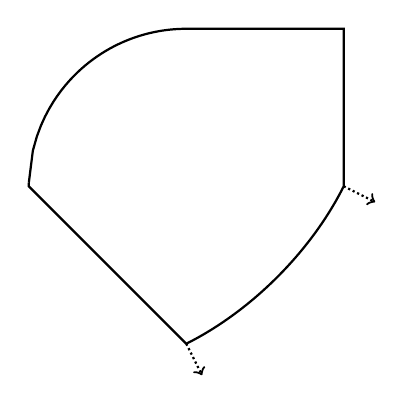
\begin{tikzpicture}[scale=2]
      \draw[thick]
      (-1, 0.02) to (-1, 0) to (0, -1)
      plot[domain=0:1, samples=40] ({\x}, {\x/2 - sqrt(4 - 3 * \x^2) / 2} )
      (1, 0) to (1, 1) to (0, 1)
      plot[domain=0:1, samples=40] ({-\x}, {sqrt(1 - \x^2)} );
      \draw[thick, densely dotted, ->] (0, -1) to (0.1, -1.2);
      \draw[thick, densely dotted, ->] (1, 0) to (1.2, -0.1);
    \end{tikzpicture}
    \caption{Set $\mathcal{S}$ defined by \eqref{eq:pieceprimal}.}
    \label{fig:pieceprimal}
  \end{subfigure}%
  \hfill%
  \begin{subfigure}[b]{0.49\textwidth}
    \centering
    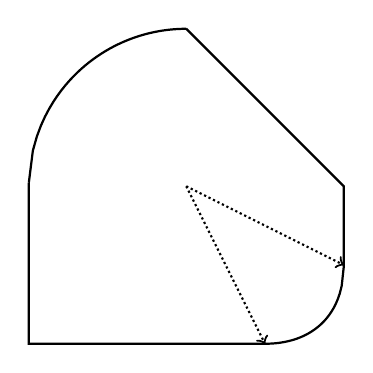
\begin{tikzpicture}[scale=2]
      \draw[thick] %
      (-1, 0.02) to (-1, -1) to (0.5, -1)
      plot[thick, domain=0.5:1, samples=40] ({\x}, {-\x/2 - sqrt(3 - 3 * \x^2) / 2} )
      (1, -0.52) to (1, 0) to (0, 1)
      plot[thick, domain=0:1, samples=40] ({-\x}, {sqrt(1 - \x^2)} );
      \draw[thick, densely dotted, ->] (0, 0) to (0.5, -1);
      \draw[thick, densely dotted, ->] (0, 0) to (1, -0.5);
    \end{tikzpicture}
    \caption{Set $\polar{\mathcal{S}}$ defined by \eqref{eq:piecepolar}.}
    \label{fig:piecepolar}
  \end{subfigure}
  \caption{Illustration for sets $\mathcal{S}$ and $\polar{\mathcal{S}}$ defined in \exemref{piecequad}.}
  \label{fig:example}
\end{figure}

\begin{myexem}
  \label{exem:piecequad}
  Consider the piecewise semi-ellipsoidal set defined by
  \begin{equation}
    \label{eq:pieceprimal}
    \gauge(\mathcal{S}, x) =
    \begin{cases}
      |x| & \text{ if } 0 \le y \le x,\\
      |y| & \text{ if } 0 \le x \le y,\\
      \sqrt{x^2 + y^2} & \text{ if } x \le 0 \le y,\\
      |x + y| & \text{ if } x, y \le 0,\\
      \sqrt{x^\Tr Q_5 x} & \text{ if } y \le 0 \le x.
    \end{cases}
  \end{equation}
  where $x^\Tr Q_5 x = x^2 - xy + y^2$.
  The polar set is also piecewise semi-ellipsoidal:
  \begin{equation}
    \label{eq:piecepolar}
    \gauge(\polar{\mathcal{S}}, x) =
    \begin{cases}
      |x + y| & \text{ if } 0 \le x, y,\\
      \sqrt{x^2 + y^2} & \text{ if } x \le 0 \le y,\\
      |x| & \text{ if } x \le y \le 0,\\
      |y| & \text{ if } y \le x, 2x + y \le 0,\\
      \sqrt{x^\Tr Q_5^{-1} x} & \text{ if } 2x + y \ge 0, x + 2y \le 0,\\
      |x| & \text{ if } x + 2y \ge 0, y \ge 0.
    \end{cases}
  \end{equation}
  where $x^\Tr Q_5^{-1} x = (4/3) \cdot (x^2 + xy + y^2)$.

  Note that the partition $\mathcal{P}_i$ of $\polar{\mathcal{S}}$ does
  not only depend on the conic partition of $\mathcal{S}$, it also depends on the
  value of the matrices $Q_i$.

  For instance, the cone defined by $2x + y \ge 0, x + 2y \ge 0$
  is the conic hull of the gradient of $\sqrt{x^2 - xy + y^2}$ evaluated
  at $(0, -1)$ and $(1, 0)$ as shown in dotted arrows in \figref{example}.
  The gradients are obtained by multiplying $(0, -1)$ and $(1, 0)$
  by the matrix $Q_5$.
  This illustrates why the partition of the polar is the image of
  the original partition under $Q_5$.
\end{myexem}



\implementations{\jlpkg{SetProg}.}

\section{Semialgebraic sets}
\label{sec:algebraic}

\begin{mydef}[{\cite[Definition~2.1.4]{bochnak2013real}}]
  A \emph{semialgebraic subset} of $\R^n$ is a set of the form
  \[ \bigcup_{i=1}^s \setbuild{x \in \R^n}{p_i(x) < 0, i = 1, \ldots, m_j, f_i(x) = 0, i = 1, \ldots, r_j} \]
  where $p_i, f_i$ are polynomials.
\end{mydef}

\begin{mydef}[{\cite[Definition~2.7.1]{bochnak2013real}}]
  A \emph{basic closed semialgebraic subset} of $\R^n$ is a set of the form
  \begin{equation}
    \label{eq:bcsa}
    \setbuild{x \in \R^n}{p_i(x) \ge 0, i = 1, \ldots, m}
  \end{equation}
  where $p_1, \ldots, p_m$ are polynomials.
\end{mydef}

\begin{mytheo}[{Finiteness Theorem~\cite[Theorem~2.7.2]{bochnak2013real}}]
  A closed semialgebraic set is a finite union of basic closed semialgebraic sets.
\end{mytheo}

One sees immediately that the family of semialgebraic sets is closed under union and intersection.
Similarly to \theoref{fourier_motzkin}, it is also has the remarkable property of being closed under projections.
\begin{mytheo}[{Tarski-Seidenberg~\cite[Theorem~2.2.1]{bochnak2013real}}]
  \label{theo:tarski_seidenberg}
  The projection of a semialgebraic set on the space of a subset of its coordinates is a semialgebraic set.
\end{mytheo}

\begin{mycoro}
  \label{coro:polarsemialg}
  The polar of a convex semialgebraic set is semialgebraic.
  \begin{proof}
    Let $\mathcal{S} \subseteq \R^n$ be a convex semialgebraic set,
    the set
    \[ \mathcal{S} \times \polar{\mathcal{S}} = \setbuild{(x, y) \in \R^{2n}}{\la x, y \ra \le 1, x \in \mathcal{S}} \]
    is semialgebraic as $\mathcal{S}$ is semialgebraic
    and $\la x, y \ra$ is a polynomial in $x, y$.
    As $\polar{\mathcal{S}}$ is a projection of this set,
    it is semialgebraic by \theoref{tarski_seidenberg}.
  \end{proof}
\end{mycoro}

When a basic closed semialgebraic set can be described by equalities only,
it is called an \emph{algebraic set} or \emph{variety}.
\begin{mydef}
  A \emph{variety} of $\R^n$ is a set of the form
  \begin{equation}
    \label{eq:variety}
    \setbuild{x \in \R^n}{p_i(x) = 0, i = 1, \ldots, m}
  \end{equation}
  where $p_1, \ldots, p_m$ are polynomials.
\end{mydef}

\subsection{Varieties and the Nullstellensatz}

Given a variety $\mathcal{V}$ as defined in \eqref{eq:variety},
the product of any of the polynomials $p_i$ with any polynomial is nonnegative on $I$.
The set of polynomials that can be certified to be zero by summing
such products is called the \emph{ideal} generated by the polynomials $p_i$.

\begin{mydef}[{Ideal \cite[Definition~1.4.2, Lemma~1.4.3]{cox2015groebner}}]
  Given polynomials $p_1(x), \ldots, p_m(x)$, the \emph{ideal} generated by
  the polynomials $p_i$ is set
  \begin{equation}
    \label{eq:ideal}
    \la p_1, \ldots, p_m \ra \eqdef
    \setbuild{q}{q = \sum_{i = 1}^m c_i p_i, c_i \in \mathcal{C}[x]}.
  \end{equation}
\end{mydef}

Given an ideal $I = \la p_1, \ldots, p_m \ra$, let $V(I)$ be the variety defined in \eqref{eq:variety}.
Given a variety $\mathcal{V}$, the set of polynomials vanishing for every point of the variety is denoted $I(\mathcal{V})$ and is an ideal.

\begin{mytheo}[{Hilbert's Nullstellensatz~\cite[Theorem~2]{cox2015groebner}}]
  Consider the ideal $I = \la p_1, \ldots, p_m \ra$.
  A polynomial $q \in I(V(I))$ if and only if $q^m \in I$ for some $m \ge 1$.
\end{mytheo}

The power $m$ can be dropped if the ideal is \emph{radical}.

\begin{mydef}[{Radical ideal~\cite[Definition~2]{cox2015groebner}}]
  An ideal $I$ is \emph{radical} if $q^m \in I$ implies that $q \in I$.
\end{mydef}

\begin{mycoro}
  Consider the ideal $I = \la p_1, \ldots, p_m \ra$.
  If $I$ is radical then a polynomial $q \in I(V(I))$ if and only if $q \in I$.
\end{mycoro}

To check that a polynomial $q(x)$ belongs to an ideal $I$, the degree needed for the
coefficients $c_i$ in \eqref{eq:ideal} is unknown a priori.
Moreover, checking whether $q(x)$ can be reduced to zero via polynomial
remainder with the polynomials $p_i(x)$ is only sufficient.
However, given an ideal $I$, one can compute the \emph{Gr\"{o}bner basis}
from the polynomials $p_1, \ldots, p_m$ with the \emph{Buchberger's algorithm}, see \cite[Section~2.7]{cox2015groebner}.


Given a monomial ordering, let $\LeadingTerm(p)$ denote the leading term of $p$.
Given two polynomials in the generating basis,
a polynomial with a new leading term can potentially be created by
taking the polynomial obtained by canceling their leading terms with each other.
This polynomial is called their \emph{S-polynomial}.

\begin{mydef}[{S-polynomial \cite[Definition~2.6.4]{cox2015groebner}}]
  Given nonzero polynomials $p, q$, let $x^\alpha$
  be the least common multiplier of their leading terms.
  The \emph{S-polynomial} of $p$ and $q$ is
  \[ \frac{x^\alpha}{\LeadingTerm(p)} p - \frac{x^\alpha}{\LeadingTerm(q)} q. \]
\end{mydef}

By repeatedly adding the remainder of the S-polynomial modulo the polynomials of a generating basis
for each pair of polynomials in the basis if the remainder is nonzero,
we converge, after finitely many additions, to a \emph{Gr\"{o}bner basis}.
This is the procedure underlying the \emph{Buchberger's algorithm}.

\begin{mydef}[{Gr\"{o}bner basis~\cite[Definition~2.5.5]{cox2015groebner}}]
  The set of polynomials $\{p_1, \ldots, p_m\}$ is a \emph{Gr\"{o}bner basis}
  if
  \begin{equation}
    \label{eq:groebner}
   \la \LeadingTerm(p_1), \ldots, \LeadingTerm(p_m) \ra = \la \LeadingTerm(p) \mid p \in \la p_1, \ldots, p_m \ra.
  \end{equation}
\end{mydef}

The ideal generated by the Gr\"{o}bner basis computed by the Buchberger's algorithm is $I$ as well but
a polynomial belongs to the ideal if and only if its remainder modulo the polynomials
of the Gr\"{o}bner basis is zero.
Therefore, if $I$ is radical then $q \in I(V(I))$ if and only if its remainder modulo
the Gr\"{o}bner basis is zero.
This gives an algorithmic way to decide the whether $q \in I(V(I))$
for a radical ideal $I$.
The downside of this approach is that computing Gr\"{o}bner basis through the
Buchberger's algorithm can be computationally intensive as the degree of the polynomials
considered by the Buchberger's algorithm is not known a priori in general.

\subsubsection{Computing the elements of zero-dimensional varieties}
\label{sec:solvealg}

A second application of Gröbner basis that is relevant to this thesis is
determining whether $V(I)$ is zero-dimensional and,
if it is the case, determining the (finitely many) elements of $V(I)$.
As shown by the following result, the variety $V(I)$ has finitely many elements
if and only if $\R[x] / I$ is finite-dimensional.

\begin{mytheo}[{\cite[Theorem~5.3.6]{cox2015groebner}}]
  The set $V(I)$ is a zero-dimensional if and only if
  the quotient ring $\R[x] / I$ is finite-dimensional.
\end{mytheo}

By \eqref{eq:groebner}, the monomial basis $b$ of $\R[x] / I$ is directly computable
from the Gr\"{o}bner basis.
The remainder of a polynomial modulo the Gr\"{o}bner basis is a polynomial of $\R[x] / I$
hence if $V(I)$ is zero-dimensional, it can be represented as a finite vector of the coordinates in $b$.
Given the monomial basis of $\R[x] / I$, we define the multiplication matrices
of $I$ as the $n$ matrices $M_{x_i}$ for each variable $x_i$ such that
the $j$th column of $M_{x_i}$ is the vector of coordinates of the remainder
of $x_i b_j$ in $b$.
It turns out that the multiplication matrices can be simultaneously diagonalized.
That is, there exists some matrix $Z$ such that $Z^* M_{x_i} Z$ is upper triangular,
this is called the Schur decomposition of $M_{x_i}$.
The diagonal elements of $Z^* M_{x_i} Z$ are the eigenvalues of $M_{x_i}$ and
the eigenvalues corresponding to the same column of $Z$ form the elements of $V(I)$.
There are several ways to obtain these elements of numerically using the multiplication
matrices.
An approach presented in \cite{manocha1995algorithms} is to sample a random convex combination $M$ of the multiplication matrices $M_{x_i}$.
As it is a convex combination of the matrices $M_{x_i}$, it also admits the same eigenvectors.
Let $M = Z T Z^*$ be the Schur decomposition of the matrix $M$.
Each column $q$ of $Z$ provides the element $a \in V(I)$ with $a_i = q^\Tr M_{x_i} q$.
Numerically, there is an important subtlety:
A solution of multiplicity $m$ will is given $m$ times in the eigenvalues of $M_{x_i}$.
However, the numerical eigenvalues in $T$ will not be equal due to inaccuracy in the floating point representation of $M$ and/or the computation of the Schur decomposition.
Interestingly, as shown in \cite[Section~4.1]{manocha1995algorithms},
the $m$ eigenvalues will be around the correct eigenvalue, at a same distance which is function of the perturbations induced by numerics.
Moreover, the arithmetic mean of the $m$ eigenvalues will cancel these inaccuracies and give an accurate estimation of the correct eigenvalues.
For this reason, the eigenvalues close to each other are clustered by taking their mean values and
the element $a \in V(I)$ is computed as the mean of $q_j^\Tr M_{x_i} q_j$ for the eigenvectors $q_j$ corresponding to each eigenvalue of the cluster.

\begin{myexem}
  \label{exem:4normpolar}
  Consider $\mathcal{S} = \polyset[x_1^4 + x_2^4]$, the unit ball of the 4-norm.
  In this example, we show how to use Gr\"{o}bner basis to find the
  face exposed by a point $y \in \polar{\mathcal{S}}$ such that $2y_1 = y_2$.
  By \propref{normal}, the face $\{x\}$ is exposed by the point $\grad (x_1^4 + x_2^4) = (4x_2^3, 4x_2^3)$
  of the $\polar{\mathcal{S}}$.
  So the point $x$ we are looking for is such that $x_1^4 + x_2^4 = 1$
  and $4x_1^3 = 8x_2^3$.
  We define this variety with \jlpkg{SemialgebraicSets} as follows:
\begin{minted}{Julia}
using DynamicPolynomials
@polyvar x[1:2]
p = 1//1 * x[1]^4 + 1//1 * x[2]^4
∇p = differentiate(p, x)
using SemialgebraicSets
V = @set p == 1 && 2∇p[1] == ∇p[2]
\end{minted}
  The Gr\"{o}bner basis of this variety
  \[ V = \la
    x_1^3 - 2x_2^3,
    x_1x_2^3 + \frac{1}{2}x_2^4 - \frac{1}{2},
    x_2^6 - \frac{4}{17}x_1^2 + \frac{2}{17}x_1x_2 - \frac{1}{17}x_2^2
  \ra \]
  is obtained with the Buchberger's algorithm as follows:
\begin{minted}{Julia}
gröbnerbasis(V.I.p)
\end{minted}
  As the leading term of the first polynomial of the basis is $x_1^3$,
  and the leading term of the third one is $x_2^6$, we see that
  for all monomial of the monomial basis $b$ of $\R[x] / I$,
  exponent of $x_1$ is at most 2 and the exponent of $x_2$ is at most 5.
  Removing all monomials that are multiple of $x_1x_2^3$, we obtain
  \[
    b = (x_2^5,
     x_1^2x_2^2,
     x_2^4,
     x_1^2x_2,
     x_1x_2^2,
     x_2^3,
     x_1^2,
     x_1x_2,
     x_2^2,
     x_1,
     x_2,
     1)
  \]
  as follows:
\begin{minted}{Julia}
b = monomialbasis(V.I)[2]
\end{minted}
  The first column of the moment matrix $M_{x_1}$ is obtained as follows:
  First, we get $q(x) = -8/17x_1^2 + 16/17x_1x_2 + 2/17x_2^2$, the remainder of
  $x_1b_2$ modulo the Gr\"{o}bner basis,
  then we get the coordinates of $q$ in the basis $b$:
  \[ (0, 0, 0, 0, 0, 0,
     -8/17,
     16/17,
      2/17,
      0, 0, 0)
  \]
  as follows:
\begin{minted}{Julia}
q = rem(x[1] * b[1], equalities(V))
coefficients(q, b)
\end{minted}
  The elements
  $((-0.73008,  %
     -0.91984), %
    ( 0.73008,
      0.91984))$
  are computed as:
\begin{minted}{Julia}
els = collect(V)
\end{minted}
  The polar point exposing the element in the nonnegative orthant is
  $(0.38914,   %
    0.77828)$, %
  as obtained with:
\begin{minted}{Julia}
normal = [∇pi(x => els[2]) for ∇pi in ∇p]
polar = normal / els[2]'normal
\end{minted}
  This is illustrated in \figref{4normpolar}.

\begin{figure}[!ht]
  \centering
  \begin{tikzpicture}[scale=2]
    \draw[thick]
    plot[domain=-1:1, samples=120] ({\x}, {(1 - (\x)^4)^(1/4)})
    plot[domain=-1:1, samples=120] ({\x}, {-(1 - (\x)^4)^(1/4)})
    (1, -0.24) to (1, 0.24);
    \draw [thick, densely dotted, ->] (0.9198, 0.73) to (1.6981, 1.1192);
    \draw [thick, densely dotted, ->] (-0.9198, -0.73) to (-1.6981, -1.1192);
    \draw[fill] (0.9198, 0.73) circle (.03);
    \draw[fill] (-0.9198, -0.73) circle (.03);
    \draw [dashed, ->] (0, 0) to (1.2, 0) node[above] {$x_1$};
    \draw [dashed, ->] (0, 0) to (0, 1.2) node[left] {$x_2$};
  \end{tikzpicture}
  \caption{Illustration for \exemref{4normpolar}.}
  \label{fig:4normpolar}
\end{figure}

\end{myexem}

We just showed how to compute the elements of a variety by computing
first the Gr\"{o}bner basis and then the multiplication matrices.
The drawback of this method is first that the computation of the Gr\"{o}bner basis
can be computationally demanding and second that it is not numerically stable.
The Gr\"{o}bner basis can be computed in exact arithmetic but this makes the computation
even more demanding and this is not an option when the coefficients of the polynomials
are not known accurately as it is the case in \secref{atom}.
For linear systems, the Gr\"{o}bner basis computation reduces to the Gauss elimination
which is not the method used to compute the solution of linear systems
because of its poor numerical performances.
For linear systems, the case is simpler as we do not need to consider polynomials of higher degree because the remainder of S-polynomials is always linear.
However, for algebraic systems of higher degree, the numerical computation of the remainder of the S-polynomials
lead to rounding errors in floating point arithmetic.

One solution suggested in \cite{dreesen2009polynomial} is to somehow keep the S-polynomials obtained without taking the remainder.
By stacking all the polynomials generated in a large matrix, the singular value decomposition (SVD) is then used
instead of polynomial division, as the SVD is numerically stable.

A more orthogonal approach is to find the elements of the variety $V(I)$
via homotopy continuation~\cite{li2003solving,breiding2018homotopycontinuation}.
This consists in defining an algebraic variety,
parametrized by a parameter $t$,
such that $V(I)$ is recovered by setting $t = 0$ and
setting $t = 1$ gives a variety for which the elements are known.
The approach then starts from the elements at $t = 1$ and
follows the path taken by the elements when $t$ is varied continuously from $t = 1$
to $t = 0$.
This path-following method varies $t$ slightly and then adjust the value of the
elements of the varieties for this new value of $t$ using the Newton method,
similarly to the interior-point path-following scheme mentioned in \secref{sdp}.

\subsection{Basic semialgebraic sets and the Positivstellensatz}

Given a basic closed semialgebraic set $\mathcal{K}$ as defined in \eqref{eq:bcsa},
the product of any subset of the polynomials $p_i$ is nonnegative on $K$
as well as their product with a \emph{sum-of-squares} polynomial.
\begin{mydef}
  \label{def:sos}
  We say that a polynomial is a \emph{sum-of-squares} (SOS) if there exist
  polynomials $q_1, \ldots, q_M$ such that
  \[ p(x) = \sum_{k=1}^Mq_k^2(x). \]
\end{mydef}

The set of polynomials that can be certified to be nonnegative by summing
such products is called the \emph{preorder}.

\begin{mydef}[Preorder]
  Given polynomials $p_1(x), \ldots, p_m(x)$, the \emph{preorder} generated by
  the polynomials $p_i$ is set
  \begin{equation}
    \label{eq:preorder}
    \preorder(p_1, \ldots, p_m) \eqdef
    \setbuild{q}{q = \sum_{I \subseteq [m]} s_I \prod_{i \in I} p_i, s_I \in \Sosinf}
  \end{equation}
  where $\Sosinf$ denotes the set of SOS polynomials.
\end{mydef}

\begin{myprop}
  \label{prop:preorder}
  If a polynomial $q \in \preorder(p_1, \ldots, p_m)$
  then $q(x) \ge 0$ for all $x \in K$ where $K$ is the basic closed semialgebraic
  set defined in \eqref{eq:bcsa}.
\end{myprop}

\begin{myprop}
  \label{prop:preordersplit}
  A polynomial $q \in \preorder(p_1, \ldots, p_m)$ if only if there exists
  $q_1, q_2 \in \preorder(p_1, \ldots, p_{m-1})$ such that
  $q = q_1 + p_mq_2$.
\end{myprop}

\begin{mytheo}[{\cite[Theorem~4.4.2]{bochnak2013real}}]
  \label{theo:positiv}
  Consider the set
  \[ K = \setbuild{x \in \R^n}{f_i(x) \ge 0, \forall i \in [m_f], g_j(x) \neq 0, \forall j \in [m_g], h_k(x) = 0, \forall k \in [m_h]}. \]
  The set $K$ is empty if and only if there exists $f \in \preorder(f_1, \ldots, f_{m_f})$,
  $g$ in the monoid generated by $g_1, \ldots, g_{m_g}$ (see \defref{monoidgen}) and
  $h \in \la h_1, \ldots, h_{m_h} \ra$ such that $f + g^2 + h = 0$.
\end{mytheo}

If $m_g = 0$ in \theoref{positiv}, the monoid generated by $g_1, \ldots, g_{m_g}$ is the singleton $\{1\}$ hence we have the following corollary.

\begin{mycoro}
  \label{coro:positiv0}
  Consider the set
  \[ K = \setbuild{x \in \R^n}{f_i(x) \ge 0, \forall i \in [m_f], h_k(x) = 0, \forall k \in [m_h]}. \]
  The set $K$ is empty if and only if there exists $f \in \preorder(f_1, \ldots, f_{m_f})$,
  and
  $h \in \la h_1, \ldots, h_{m_h} \ra$ such that $f + h = -1$.
\end{mycoro}

We have already seen the particular case of \cororef{positiv0} for affine $f_i$ and $h_k$ in \propref{affsubset}.\ref{enum:empty_aff}.

If $m_g = 1$ in \theoref{positiv}, the monoid generated by $g_1, \ldots, g_{m_g}$ is the set of powers of $g_1$ hence we have the following corollary.

\begin{mycoro}
  \label{coro:positiv1}
  Consider the set
  \[ K = \setbuild{x \in \R^n}{f_i(x) \ge 0, \forall i \in [m_f], g(x) \neq 0, h_k(x) = 0, \forall k \in [m_h]}. \]
  The set $K$ is empty if and only if there exists $f \in \preorder(f_1, \ldots, f_{m_f})$, $k \in \mathcal{N}$
  and
  $h \in \la h_1, \ldots, h_{m_h} \ra$ such that $f + g^{2k} + h = 0$.
\end{mycoro}

The Positivstellensatz follows from \cororef{positiv0}, \cororef{positiv1} and \propref{preordersplit}.

\begin{mycoro}[{Positivstellensatz \cite[Corollary~4.4.3]{bochnak2013real}}]
  \label{coro:positiv}
  Consider the set
  \[ K = \setbuild{x \in \R^n}{p_i(x) \ge 0, \forall i \in [m_p], h_k(x) = 0, \forall k \in [m_h]} \]
  and a polynomial $q(x)$.
  \begin{enumerate}
    \item We have $q(x) \ge 0$ for all $x \in K$ if and only if there exists
      $k \in \mathcal{N}$, $q_1(x), q_2(x) \in \preorder(p_1, \ldots, p_{m_p})$ and $h \in \la h_1, \ldots, h_{m_h} \ra$ such that
      $qq_1 = q^{2k} + q_2 + h$.
    \item We have $q(x) > 0$ for all $x \in K$ if and only if there exists
      $q_1(x), q_2(x) \in \preorder(p_1, \ldots, p_{m_p})$ and $h \in \la h_1, \ldots, h_{m_h} \ra$ such that
      $qq_1 = 1 + q_2 + h$.
    \item We have $q(x) = 0$ for all $x \in K$ if and only if there exists
      $k \in \mathcal{N}$, $p(x) \in \preorder(p_1, \ldots, p_{m_p})$ and $h \in \la h_1, \ldots, h_{m_h} \ra$ such that
      $0 = q^{2k} + p + h$.
  \end{enumerate}
\end{mycoro}

Schm{\"u}dgen's showed in \cite{schmudgen1991thek} that
if the set $K$ is compact, then we can choose $q_1 = 1$ in the second
certificate of \cororef{positiv} and we do not need the term $1$ in the right-hand side.

\begin{mytheo}[{Schm{\"u}dgen's certificate~\cite[Corollary~3]{schmudgen1991thek}}]
  \label{theo:schmudgen}
  Consider a polynomial $q(x)$ and basic closed semialgebraic set $K$ of the form \eqref{eq:bcsa} that is compact.
  We have $q(x) > 0$ for all $x \in K$ if and only if
  $q(x) \in \preorder(p_1, \ldots, p_m)$.
\end{mytheo}

A subset of the preorder is given by the quadratic module.

\begin{mydef}[Quadratic module]
  \label{def:qmodule}
  Given polynomials $p_1(x), \ldots, p_m(x)$, the \emph{qmodule} generated by
  the polynomials $p_i$ is set
  \begin{equation}
    \label{eq:qmodule}
    \qmodule(p_1, \ldots, p_m) \eqdef
    \setbuild{q}{q = \sum_{i \in [m]} s_i p_i, s_i \in \Sosinf}.
  \end{equation}
\end{mydef}

As the quadratic module is a subset of the preorder, the following
proposition follows directly from \propref{preorder}.

\begin{myprop}
  \label{prop:qmodule}
  If a polynomial $q \in \qmodule(p_1, \ldots, p_m)$
  then $p(x) \ge 0$ for all $x \in K$ where $K$ is the basic closed semialgebraic
  set defined in \eqref{eq:bcsa}.
\end{myprop}

Putinar showed in \cite{putinar1993positive} that if the compactness of the set
can be shown with the qmodule certificate then the Schm{\"u}dgen's certificate presented in \theoref{schmudgen} than be simplified further.

\begin{mydef}[Arichmedean]
  A quadratic module is \emph{Arichmedean} if there exists $\rho \ge 0$ such that
  $\rho - x_1^2 - \ldots - x_n^2$ belongs to the quadratic module.
\end{mydef}

\begin{mytheo}[{Putinar's certificate~\cite{putinar1993positive}}]
  Consider a polynomial $q(x)$ and a basic closed semialgebraic set $K$ of the form \eqref{eq:bcsa}
  such that the quadratic module $\qmodule(p_1, \ldots, p_m)$ is Arichmedean.
  We have $q(x) > 0$ for all $x \in K$ if and only if
  $q(x) \in \qmodule(p_1, \ldots, p_m)$.
\end{mytheo}

When the polynomials $q(x)$ and $p_i(x)$ are affine, the quadratic module certificate
is necessary and sufficient for the nonnegativity of $q(x)$ over the polyhedron
without any assumption on boundedness. Furthermore, the sum-of-squares polynomials
$s_i(x)$ of \eqref{eq:qmodule} can be chosen to be nonnegative numbers.
This results in \propref{hinhrep}.

\subsubsection{Copositivity}

A typical application of the Positivstellensatz is the verification of
the positivity of a quadratic polynomial over a polyhedron.
The canonical instance of this problem is checking the copositivity of a symmetric matrix.
\begin{mydef}[Copositivity]
  A matrix $Q \in \SymK$ is \emph{copositive} if
  $x^\Tr Q x \ge 0$ for all $x \in \R^n_+$.
\end{mydef}

While checking copositivity of a matrix is co-NP-complete~\cite{murty1987some},
we see in this section that a sufficient condition such as \propref{copos} can be encoded as a LMI
and a necessary and sufficient condition is achieved through a hierarchy of LMIs of increasingly larger size.

A commonly used sufficient condition checks the membership of the polynomial
$q(x) = x^\Tr Q x$ in a subset of the preorder generated by $x_1, \ldots, x_n$
when only subsets $I \subseteq [n]$ of two elements are considered in \eqref{eq:preorder}.
In the matrix form, the product $x_ix_j$ corresponds to the off-diagonal entry at row $i$ and column $j$ of a matrix.
Therefore, the following property follows directly from \propref{preorder}.
\begin{myprop}[{\cite[Section~3.6.1]{blekherman2012semidefinite}}]
  \label{prop:copos}
  Consider a symmetric matrix $Q \in \SymK$.
  If there exists a matrix $P \in \SymK$ with zero diagonal entries
  and nonnegative off-diagonal entries such that $Q \succeq P$ then
  $Q$ is copositive.
\end{myprop}

This is generalized to the following proposition for an arbitrary polyhedral cone.

\begin{myprop}
  \label{prop:conepos}
  Consider a polyhedral cone $\Pset$ with homogeneous H-representation
  given by $(a_i)_{i=1}^\ineqnum$
  and a symmetric matrix $Q \in \SymK$.
  If there exists nonnegative $\lambda_{ij} \in \R_+$ such that
  \[ Q \succeq \sum_{i \neq j} \lambda_{ij} (a_ia_j^\Tr + a_ja_i^\Tr) \]
  then for all $x \in \Pset$, we have $x^\Tr Q x \ge 0$.
\end{myprop}

\begin{myrem}
  \label{rem:copos}
  While \propref{copos} and \propref{conepos} only provide a sufficient condition,
  a necessary condition can be obtained using a hierarchy of
  semidefinite programs of increasingly larger size by increasing the degree of $q_1$ and $q_2$ in \cororef{positiv}; see \cite[Chapter~5]{parrilo2000structured} for more details.
\end{myrem}


\subsubsection{S-procedure}

In this section, we consider the case of quadratic $q(x)$ and $p_i(x)$.
The \emph{lossy S-procedure} is simply the special case of \propref{qmodule}
for quadratic forms and scalar numbers for the sum-of-squares polynomials
$s_i(x)$ of \eqref{eq:qmodule}.
\begin{myprop}[Lossy S-procedure]
  \label{prop:lossysproc}
  Consider symmetric matrices $Q, P_1, \ldots, P_m \in \SymK$, the polynomials
  $p_i(x) = x^\Tr P_i x$ and the basic closed semialgebraic set defined in \eqref{eq:bcsa}.
  If
  \[ Q \succeq \lambda_1 P_1 + \cdots + \lambda_m P_m \]
  then $x^\Tr Q x \ge 0$ for all $x \in K$.
\end{myprop}

When $m = 1$, under a \emph{constraint qualification} condition,
the S-procedure certificate is necessary.

\begin{mytheo}[{Lossless S-procedure \cite{polik2007survey}}]
  \label{prop:sproc}
  Given two symmetric matrices $Q_1, Q_2 \in \SymK$,
  the existence of a $\lambda \geq 0$ such that the matrix $\lambda Q_{1} - Q_{2}$ is positive semidefinite
  is sufficient for the following proposition to hold:
  \begin{quote}
    for all $x \in \R^n$, $x^\Tr Q_1 x \leq 0 \Rightarrow x^\Tr Q_2 x \leq 0$.
  \end{quote}
  Moreover, if there exists $x \in \R^n$ such that $x^\Tr Q_1 x > 0$ then this condition is also necessary.
\end{mytheo}

In case $Q_1, Q_2$ are of a specific form, the $\lambda$ of \propref{sproc}
can be chosen to be $1$.
This is the case for instance for \propref{ellincl}.

\subsection{Polysets}

We consider in this section the sets that are the sublevel
set of a nonnegative \emph{homogeneous}\footnote{A polynomial is homogeneous if all its monomials have the same total degree.} polynomial of degree $2d$ for some positive integer $d$.
We refer to these sets as \emph{polysets of degree $2d$}
and denote it by
\begin{equation}
  \label{eq:polyset}
  \polyset = \setbuild{x \in \R^n}{p(x) \leq 1}.
\end{equation}
where $p$ is a homogeneous polynomial of degree $2d$.
The family of ellipsoids presented in \secref{ell}
is exactly the family of polysets of degree 2.
We detail in this section how to generalize the results on ellipsoids to polysets of higher degree.

The gauge function and gauge-like function of degree $2d$ of the polyset are
\begin{align}
  \label{eq:gaugepolyset}
  \gauge(\polyset, x) & = \sqrt[2d]{p(x)} &
  \gauge_{2d}(\polyset, x) & = \frac{p(x)}{2d}.
\end{align}
Note that the convexity of $\gauge(\polyset, x)$ and $\gauge_{2d}(\polyset, x)$ are equivalent by \cite[Corollary~15.3.1]{rockafellar2015convex}.

As a consequence of \propref{gaugelikeincl} and \eqref{eq:gaugepolyset},
the inclusion between polysets is verified using the following property.
\begin{myprop}
  \label{prop:polysetincl}
  Consider two polysets $\polyset[p_1], \polyset[p_2]$ of degree $2d$.
  The inclusion $\polyset[p_1] \subseteq \polyset[p_2]$ is equivalent to
  $p_1(x) \ge p_2(x)$ for all $x \in \R^n$.
\end{myprop}

Well-known examples of polysets are the $(2d)$-unit balls.
The gauge function of the $(2d)$-unit ball is the $L^{2d}$ norm.
The $L^{p}$ norm is convex for any $p \ge 1$ and by \propref{polarnorm} its polar
is the $q$-unit ball for $q \ge 1$ such that $1/p + 1/q = 1$.
Hence the $(2d)$-unit ball is convex for any positive integer $d$ and its polar is the $(2d)/(2d-1)$-unit ball.
This shows that, except for $d = 1$, the polar of a polyset is not necessarily a polyset,
even if it is always a semialgebraic set by \cororef{polarsemialg}.

\subsection{Piecewise polysets}
\label{sec:piecepoly}

Similarly to the piecewise semi-ellipsoidal sets introduced in \secref{pieceell},
we define in this section the family of \emph{piecewise polysets}.

\begin{mydef}[Piecewise semi-ellipsoidal sets]
  \label{def:piecepoly}
  A closed convex set $\mathcal{S} \subseteq \R^n$ containing the origin is said to be a \emph{piecewise polyset} of degree $2d$ if there exists
  a conic partition $(\mathcal{P}_i)_{i=1}^m$
  and convex nonnegative homogeneous polynomials $p_i(x)$ of degree $2d$ for $i = 1, \ldots, m$,
  such that
  \begin{align}
    \notag
    \gauge(\mathcal{S}, x) & =
      \sqrt[2d]{p_i(x)} & \text{ if } x \in \mathcal{P}_i,
    \\
    \label{eq:piecepolycont}
    p_i(x) & = p_j(x), \quad \forall i, j \in \mathcal{N}, x \in \mathcal{P}_i \cap \mathcal{P}_j\\
    \label{eq:piecepolyconv}
    n_{ij}^\Tr \grad p_i(x) & \ge n_{ij}^\Tr \grad p_j(x), \quad \forall i, j \in \mathcal{N}, x \in \mathcal{P}_i \cap \mathcal{P}_j.
  \end{align}
\end{mydef}
Note that without \eqref{eq:piecepolycont} and \eqref{eq:piecepolyconv}, the 1-sublevel set of
the piecewise semi-ellipsoidal function may be non-convex.
The condition \eqref{eq:piecepolycont} ensures the continuity of the function
and \eqref{eq:piecepolyconv} ensures its convexity.
Note that the convexity of $\gauge$ and $\gauge_{2d}$ are equivalent by \cite[Corollary~15.3.1]{rockafellar2015convex}.

This family generalizes both polysets and piecewise semi-ellipsoids.
Indeed, if $m = 1$ and $\mathcal{P}_1 = \R^n$, we recover the family of polysets and
if $d = 1$, we recover the family of piecewise semi-ellipsoids.

The piece $\mathcal{S} \cap \mathcal{P}_i$ is basic closed semialgebraic as it is the intersection of the polyset with $p_i(x)$ as gauge-like function of degree $2d$ and the set $\mathcal{S}_1$.
As $\mathcal{S}$ is the union of $\mathcal{S} \cap \mathcal{P}_i$ for each $i$, it is a closed semialgebraic set.
Therefore, its polar is semialgebraic as well.
However, it is not a piecewise polyset for $d \neq 1$
as the $2d$-unit ball is a piecewise polyset but its polar,
the $(2d)/(2d-1)$-unit ball, is not a piecewise polyset.



\chapter{Optimization}
\label{chap:opti}

\section{Conic optimization}

Set computation heavily relies on optimization algorithms for certifying membership of point in a set or the inclusion of a set in another one.
We survey in this chapter the optimization results that are used in the thesis.

In conic optimization, we term the \textit{standard conic} form:
\begin{equation}\label{eq:conic_standard_form}
    \begin{array}{rl}
        \min\limits_{x\in\mathbb{R}^N} & c^\top x\\
        \text{subject to:} & Ax = b\\
                           & x \in \mathcal{K},
    \end{array}
\end{equation}
with as dual the \textit{geometric conic} form:
\begin{equation}\label{eq:conic_geometric_form}
    \begin{array}{rl}
        \max\limits_{y\in\mathbb{R}^M} & b^\top y\\
        \text{subject to:} & c - A^\Tr y \in \mathcal{K}^*\\
                           & y\ \mathsf{free}.
    \end{array}
\end{equation}
Here, $c$ is a $N$-dimensional vector, $A$ is an $M\times N$ matrix, $b$ is an $M$-dimensional vector, and $\mathcal{K} \subseteq \mathbb{R}^N$ is a convex cone.
The cone $\mathcal{K}$ is typically the cartesian product of severel cones.

When $\mathcal{K}$ is a cartesian product of the nonnegative orthant $\R^n_+$ and the nonpositive orthant $\R^n_-$,
the conic program is called a \emph{linear program}.
The feasible set of a linear program is a polyhedron.
Considering that $\mathcal{K} = \R^N$,
for \eqref{eq:conic_standard_form}, this polyhedron is the intersection of the nonnegative orthant and the affine subspace defined by the equalities $Ax = b$.
For \eqref{eq:conic_geometric_form}, the H-representation of the polyhedron is $(A_{:,i}, b_i)_{i=1}^N$.

\begin{mydef}
  The \emph{second-order cone} (or Lorenz cone or $\ell_2$-norm cone) is the cone
  \[
    \setbuild{(t,x) \in \R_+ \times \R^n}{t \ge \lVert x \rVert_2}.
  \]
\end{mydef}

\begin{mydef}
  The \emph{rotated second-order cone} is the cone
  \begin{equation}
    \label{eq:rsoc}
    \setbuild{(t,u,x) \in \R_+^2 \times \R^n}{2tu \ge \lVert x \rVert_2^2}.
  \end{equation}
\end{mydef}

When $\mathcal{K}$ additionally contains second-order cones or rotated second-order cones,
the conic program is called a \emph{second-order cone program}.
The feasible set of a second-order cone program is the intersection between semi-ellipsoids and a polyhedron.

The problems that can be solved via second-order cone programming are
called \emph{second-order cone representable}.
For instance, \propref{memsoc} shows that the membership of a vector of
decision variables in an ellipsoid is second-order cone representable.
\begin{myprop}[{\cite[Section~3.3.1]{ben2001lectures}}]
  \label{prop:memsoc}
  Given a positive semidefinite matrix $Q \in \SymK$ and a vector $c \in \mathbb{R}^n$,
  the constraint $x \in \Ellc{Q}{c}$ is second-order cone representable.
  \begin{proof}
    Consider a Cholesky factorization $Q = L^\Tr L$,
    the inequality $(x-c)^\Tr Q (x-c) \leq 1$ can be rewritten as
    $\|L(x-c)\|_2 \leq 1$ where $\|\cdot\|_2$ is the Euclidean norm.
  \end{proof}
\end{myprop}

\subsection{Duality}

The Lagrangian function of this pair of primal-dual programs is given by
\begin{equation}
  \label{eq:Lagrangian}
  L(x, y) = y^\Tr b + c^\Tr x - y^\Tr A x.
\end{equation}

The standard conic program~\eqref{eq:conic_standard_form} is equivalent to
\[ \inf\limits_{x\in\mathcal{K}} \sup\limits_{y \in \R^M} L(x, y) \]
and the geometric conic program~\eqref{eq:conic_geometric_form} is equivalent to
\[ \sup\limits_{y\in\R^M} \inf\limits_{x \in \mathcal{K}} L(x, y). \]

\begin{myprop}[Max-min inequality]
  For any function $f(x, y):\mathcal{X} \times \mathcal{Y} \to \R$,
  for any $y \in Y$ and any $x \in X$, we have
  \begin{equation*}
    \inf\limits_{x' \in \mathcal{X}} f(x', y) \le \sup\limits_{y' \in \mathcal{Y}} f(x, y').
  \end{equation*}
  and therefore
  \begin{equation*}
    \sup\limits_{y\in\mathcal{Y}} \inf\limits_{x \in \mathcal{X}} f(x, y) \le \inf\limits_{x\in\mathcal{X}} \sup\limits_{y \in \mathcal{Y}} f(x, y).
  \end{equation*}
\end{myprop}

The \emph{weak duality} follows from this property.
\begin{mycoro}[Weak duality]
  For any feasible solution $y$ of \eqref{eq:conic_geometric_form},
  its objective value is a lower bound to the optimal value of \eqref{eq:conic_standard_form}.
  For any feasible solution $x$ of \eqref{eq:conic_standard_form},
  its objective value is an upper bound to the optimal value of \eqref{eq:conic_geometric_form}.
  Therefore, the optimal value of \eqref{eq:conic_geometric_form} is smaller than
  the optimal value of \eqref{eq:conic_standard_form}.
\end{mycoro}

An ray of \eqref{eq:conic_standard_form} is a vector $x \in \mathcal{K}$
such that $Ax = 0$.
An infeasibility ray of \eqref{eq:conic_standard_form} is a ray $x$ of \eqref{eq:conic_standard_form} such that $c^\Tr x < 0$.
A ray of \eqref{eq:conic_geometric_form} is a vector $y$ such that
$-A^\Tr y \in \mathcal{K}^*$.
An infeasibility ray of \eqref{eq:conic_geometric_form} is a
ray $y$ of \eqref{eq:conic_geometric_form} such that $b^\Tr y > 0$.

The name infeasibility ray comes from the following property
which generalize the classical Farkas' lemma in linear programming to conic programs.

\begin{myprop}[Generalized Farkas' lemma]
  \label{prop:farkas}
  The program \eqref{eq:conic_standard_form} has a infeasibility ray
  if and only if \eqref{eq:conic_geometric_form} is infeasible.
  The program \eqref{eq:conic_geometric_form} has a infeasibility ray
  if and only if \eqref{eq:conic_standard_form} is infeasible.
\end{myprop}

If \eqref{eq:conic_standard_form} (resp. \eqref{eq:conic_geometric_form})
has both a feasible solution and an infeasibility ray then
the program is unbounded.
If a program is unbounded then its dual is infeasible but
a program may be infeasible even if its dual is not unbounded.

Indeed both \eqref{eq:conic_standard_form} and \eqref{eq:conic_geometric_form} may both be infeasible.
In this case, both programs have an infeasibility ray
but none of them have a feasible solution.

The difference between \eqref{eq:conic_standard_form} and \eqref{eq:conic_geometric_form}
is called the \emph{duality} gap.
If both programs are infeasible, the duality gap is infinite.

A solution $x$ is said to be strictly feasible for \eqref{eq:conic_standard_form}
if $x$ is feasible and $x \in \inte(K)$.
A solution $y$ is said to be strictly feasible for \eqref{eq:conic_geometric_form}
if $c - A^\Tr y \in \inte(K^*)$.


The existence of a strict feasible solution is often called the \emph{Slater condition}.
The strong duality under this \emph{constraint qualification} is given by the following result.
\begin{mytheo}[Strong duality]
  If \eqref{eq:conic_standard_form} and \eqref{eq:conic_geometric_form}
  have a strictly feasible solution then the duality gap is zero.
\end{mytheo}
Strong duality may also be established by alternative methods as in \lemref{duality} for instance.





\subsection{Model transformation with bridges}
\label{sec:bridges}

In this section, we introduce the concept of model transformation with \emph{bridges}.
While the concept of model transformation is not novel,
the uniqueness of the bridging concept, newly introduced in \cite{legat2021mathoptinterface},
relies in its constraint-wise nature.
The bridge for each constraint is defined independently
which allows, as detailed in \secref{bridge_sec}, to automatically
tailor the model transformation to the capability of a given solver
even during model construction, i.e. before the full model is known.
This was implemented in the \jlpkg{MathOptInterface} Julia package
which is the solver interface used by JuMP since its version 0.19 that was
released in the 15nd of March 2019.
This section develops the bridge concept at the abstract mathematical level
and is not specific to its Julia implementation in \jlpkg{MathOptInterface} except \remref{jitbridges}.


In general, a conic model can be formulated in the form
\begin{equation}\label{eq:conic_form}
    \begin{array}{rl}
        \min\limits_{x\in\mathbb{R}^N} & c^\top x\\
        \text{subject to:} & b - Ax \in \mathcal{C}\\
                           & x \in \mathcal{K},
    \end{array}
\end{equation}
where $\mathcal{C}, \mathcal{K}$ are convex cones.
When $\mathcal{C}$ is $\{0\}^M$, this is the standard conic form and
when $\mathcal{K} = \R^N$, this is the geometric conic form.

A conic solver expects the conic program to be provided in a specific class
of conic program.
A conic optimization interface should allow the user to formulate the program
in \eqref{eq:conic_form} and perform the transformation to the form required
by the solver automatically and transparently when possible.
This allows the algorithm relying on the conic program solution to be independent
on the actual solver used.

For instance, if a solver only supports the nonnegative orthant and
one constraint in \eqref{eq:conic_form} is $b_i - A_{i,:} x \in \R_-$,
it can be replaced by $-b_i - (-A_{i,:}) x \in \R_+$.
We refer to this transformation as a constraint bridge from the cone $\R_-$ to the cone $\R_+$.
If a variable $x_i \in \R_-$, it can be substituted for $-y_i$ with $y_i \in \R_+$.
We refer to this transformation as a variable bridge.

In general, given a relation
\begin{equation}
  \label{eq:AS1S2}
  AS_1 = S_2
\end{equation}
between two cones $S_1$, $S_2$, we have
\begin{itemize}
  \item a variable bridge from $S_2$ to $S_1$ that substitutes
    $x \in S_2$ by $Ay$ where $y \in S_1$.
  \item a constraint bridge from $S_1$ to $S_2$ that replace
    a constraint $f(x) \in S_1$ into a constraint $Af(x) \in S_2$.
\end{itemize}

To provide a transparent transformation, the dual of the original
constraint should be obtained from the dual of the bridged constraint
that was transmitted to the solver.
For the constraint bridge, in the original problem, there is a constraint
$f(x) \in S_1$ in the primal program, a variable $u \in S_1^*$ in the dual program
and the term $\langle f(x), u \rangle_1$ in the Lagrangian function \eqref{eq:Lagrangian}.
In the bridged model, there is the constraint $Af(x) \in S_2$ in the primal program,
a variable $v \in S_2^*$ in the dual program and the term
$\langle Af(x), v \rangle$ in the Lagrangian function \eqref{eq:Lagrangian}.

By \eqref{eq:AS1S2} and \propref{podu}, we have
\begin{equation}
  \label{eq:S1AS2}
  S_1^* = A^\Tr S_2^*.
\end{equation}
hence $u = A^\Tr v$ is feasible for the original dual program if and only
if $v$ is feasible for the bridged dual program.
Moreover, we have
\[ \langle f(x), A^\Tr v \rangle_1 = \langle A f(x), y \rangle_2 \]
so the term in the Lagrangian function \eqref{eq:Lagrangian} is equal as well.
We conclude that the dual value $u$ should be computed as $A^\Tr v$.

For the variable bridge, a similar reasoning shows that the dual $v$ of $x \in S_2$
should be such that $A^\Tr v$ is the dual $u \in S_1^*$ of $y \in S_1$ computed by the solver.
If $A$ is invertible, this means that $v$ can be computed with $A^{-\Tr} u$.
Otherwise, there can either be no solution for the system $A^\Tr v = u$ or an affine subspace of solutions.
Note that by \eqref{eq:S1AS2}, the feasibility of $u$ in the bridged dual program implies the existence of a solution for the system $A^\Tr v = u$.
In case the set of solutions is an affine subspace of nonzero dimension, adding the additional condition $v \in S_2^*$ might leave a unique solution.

The following examples exhibit the linear relationship between the rotated second-order cone and the second-order cone.

\begin{myexem}
  \label{exem:rsoc}
  Variable and constraint bridges from rotated second-order cone to second-order cone
  and vice versa may be obtained by noticing that $2tu = (t/\sqrt{2} + u/\sqrt{2})^2 - (t/\sqrt{2} - u/\sqrt{2})^2$ hence
  \[
    2tu \ge \norm{x}_2^2
  \]
  is equivalent to
  \[
    (t/\sqrt{2} + u/\sqrt{2})^2 \ge \norm{x}_2^2 + (t/\sqrt{2} - u/\sqrt{2})^2.
  \]
  See \cite[p.~104]{ben2001lectures} for more details.
  Therefore use the linear transformation $A \eqdef (t, u, x) \mapsto (t/\sqrt{2}+u/\sqrt{2}, t/\sqrt{2}-u/\sqrt{2}, x)$.
  Note that the linear transformation is a symmetric involution (i.e. it is its own transpose and its own inverse).
  That means that the dual solution of the bridged constraint can simply be multiplied
  by $A$ to give the dual solution of the original constraint.
  As $A$ is a symmetric involution, the norm of the dual solutions are preserved by the transformation.
\end{myexem}

The following lemma follow geometrically from the right angle formed at the origin
by the rotated second-order cone.
For a similar property for the second-order cone, see \figref{socperp} or \cite[Fact~1]{fawzi2018representing}.

\begin{mylem}
  \label{lem:rsocperp}
  If the two vectors $(1, s, x), (v, u, y)$ belong to the rotated second-order cone and
  $\la (1, s, x), (v, u, y) \ra = 0$, then
  $y = -ux$ and $v = u \lVert x \rVert_2^2/2$.

  \begin{proof}
    We have
    \begin{align*}
      (1, s, x) \cdot (v, u, y) %
      & = v + s u + \la x, y \ra\\
      & \ge
      v + s u - \lVert x\lVert_2 \lVert y\lVert_2\\
      & \ge
      v + s u - 2 \sqrt{s u v}\\
      & \ge
      v + s u - 2 \frac{v + s u}{2}\\
      & = 0.
    \end{align*}
    The first inequality uses the Cauchy-Schwarz inequality,
    the second one uses \eqref{eq:rsoc} and the third one uses \propref{pmean} with $p = 1$.
    By assumption, the left-hand side is zero, hence all inequalities
    are equalities. By Cauchy-Schwarz, this means that $\exists \sigma \ge 0$ such
    that $y = -\sigma x$. By \propref{pmean}, we have $v = s u$.
    By \eqref{eq:rsoc}, we have either:
    \begin{enumerate}
      \item $\enorm{y}^2 < 2  u  v$ and $\enorm{x}^2 = 2 s = 0$:
        That implies
        that $v = 0 \cdot u = 0$ hence $\enorm{y}^2 < 0$ which is impossible.
      \item $\enorm{x}^2 < 2 s$ and $\enorm{y}^2 = 2 \cdot u \cdot v = 0$:
        we have either:
        \begin{enumerate}
          \item $u = 0$: hence $v = s \cdot u = 0$ or
          \item $v = 0$: since $s > 0$, $u = v / s = 0$.
        \end{enumerate}
         In any case, $y = 0$ and $u = v = 0$ hence the statement holds.
       \item $\enorm{x}^2 = 2 s$ and $\enorm{y}^2 = 2 u v$: we have
         $\sigma^2 \enorm{x}^2 = \enorm{y}^2 = 2 u v = 2 u^2 s$ hence
         $u = \sigma$. It follows that at $v = s u = \sigma \enorm{x}^2/2$.
    \end{enumerate}
  \end{proof}
\end{mylem}

\begin{figure}
  \centering
  \begin{tikzpicture}[scale=2]
    \draw[->] (0, -0.1) to (0, 1.5);
    \node[right] at (0, 1.5) {$t, u$};
    \draw[->] (-1.5, 0) to (1.5, 0);
    \node[above] at (1.5, 0) {$x, y$};
    \draw[dashed] (0, 0) to (1.4, 1.4);
    \draw[->] (0, 0) to (1, 1);
    \draw[dashed] (0, 0) to (-1.4, 1.4);
    \draw[->] (0, 0) to (-1, 1);
    \draw (0.1, 0.1) to (0, 0.2) to (-0.1, 0.1);
  \end{tikzpicture}
  \caption{Visualization of second order cone and complementarity slackness.
    If $(t, x), (u, y)$ belong to the second-order cone and $(t, x) \cdot (u, y) = 0$,
    then $(u, y)$ is parallel to $(t, -x)$ or $(t, x)$ is zero or $(u, y)$ is zero.
  }
  \label{fig:socperp}
\end{figure}

\begin{myexem}[Quadratic to rotated second-order cone]
  The dual transformation is trickier to obtain for the bridge from
  convex quadratic constraints into rotated second-order cone constraints.
  Given a convex quadratic constraint:
  $$\frac{1}{2}x^\Tr Q x + a^\Tr x + \beta \le 0,$$
  the symmetric matrix $Q$ is positive semidefinite as the constraint is convex.
  Consider the Cholesky decomposition $Q = U^\top U$, the constraint is
  equivalent to
  $$\lVert U x\rVert_2^2 \le 2 (-a^\Tr x - \beta)$$
  which is equivalent to the membership of the vector $(1, -a^T x - \beta, Ux)$
  to the rotated second-order cone.

  Let $z = Ux$ and $s = -a^\Tr x - \beta$ and $(v, u, y)$ be the dual solution of the rotated second-order cone constraint.
  By \lemref{rsocperp}, the complementarity slackness $(1, s, z) \cdot (v, u, y) = 0$
  implies that $v = u \lVert z \rVert_2^2/2$ and $y = -uz$.
  Moreover, the term in the Lagrangian of the bridged model is:
  \begin{align*}
    (1, s, z) \cdot (v, u, y)
    & = u (1, s, z) \cdot (\lVert z \rVert_2^2/2, 1, -z)\\
    & = u (\lVert z \rVert_2^2/2 + s - \lVert z \rVert_2^2)\\
    & = u (-\lVert z \rVert_2^2/2 + s)\\
    & = u (-\lVert Ux \rVert_2^2/2 - a^\top x - \beta)\\
    & = -u (x^T U^\Tr U x/2 + a^\Tr x + \beta).
  \end{align*}
  Therefore with the dual $-u$ of the quadratic constraint,
  the value of the term in the lagrangian is the same in both the original and bridged model.
\end{myexem}

Some constraint bridges create auxiliary variables $u$.
That is, a constraint $f(x) \in \mathcal{S}_1$ is transformed into
a constraint $Af(x) + Bu \in \mathcal{S}_2$ for some auxiliary variables $u$ where $A \in \R^{r \times n}, B \in \R^{n \times m}$.
Such bridges originate from the lifted representation of the set $\mathcal{S}_1$ in a lifted space with variables $x$ and $u$:
$x \in \mathcal{S}_1 \Leftrightarrow \exists u: Ax + Bu \in \mathcal{S}_2$.
This is equivalent to
\[
  \mathcal{S}_1 =
  \pi_{[n], n + m}
  \begin{pmatrix}
    A & B
  \end{pmatrix}^{-1}
  \mathcal{S}_2
\]
Using \propref{podu}, this is equivalent to
\[
  \mathcal{S}_1^* =
  \pi_{[n], n + m}^{-\Tr}
  \begin{pmatrix}
    A^\Tr \\ B^\Tr
  \end{pmatrix}
  \mathcal{S}_2^*
\]
or equivalently
\begin{align}
  \label{eq:bridge_proj}
  \mathcal{S}_1^* & = A^\Tr \mathcal{S}_2^* & 0 & = B^\Tr \mathcal{S}_2^*.
\end{align}

\begin{myexem}
  \label{exem:slack}
  An essential bridge needed for the standard conic form~\eqref{eq:conic_standard_form} is the slack bridge.
  This bridge transforms a constraint $f(x) \in \mathcal{S}$
  into a constraint $f(x) = y$ with $y \in \mathcal{S}$ for any set $\mathcal{S} \subseteq \R^n$.
  It relies on the relation
  \[
    x \in \mathcal{S} \Leftrightarrow
    \exists y \in \mathcal{S}, x = y
  \]
  which can be rewritten into
  \[
    \mathcal{S} =
    \pi_{[n], 2n}
    \begin{pmatrix}
      0 & I_n\\
      I_n & -I_n
    \end{pmatrix}^{-1}
    (\mathcal{S} \times \{0\}^n).
  \]
  Given a dual vector $u$ of $x \in \mathcal{S}$ in the original model and
  dual vectors
  $v$ of the constraint $y \in \mathcal{S}$
  and $w$ of the constraint $x = y$ in the bridged model,
  equation~\eqref{eq:bridge_proj} gives
  \begin{align*}
    u & = w & v & = w.
  \end{align*}
  So $u$ can be set to either $w$ or $v$.
\end{myexem}

\subsubsection{Automatic selection of bridges}
\label{sec:bridge_sec}








We already introduced the variable bridges and constraint bridges.
There is a third type of bridges called \emph{objective bridges} that can be used to transform objective functions.
Figure \ref{fig:quadratic_bridges} illustrates the possible choices to bridge a quadratic objective into a form supported by the semidefinite programming standard form~\eqref{eq:sdp_standard}.

The bridges can be nested to allow multiple transformations.
It is easy to see that as the number of constraint types and bridges increases, the number of different equivalent reformulations also increases, and choosing an appropriate reformulation becomes difficult.
We overcome the proliferation challenge by posing the question of how to transform a constraint into supported equivalents as a shortest path problem through a hyper-graph.

\begin{figure}
    \centering
    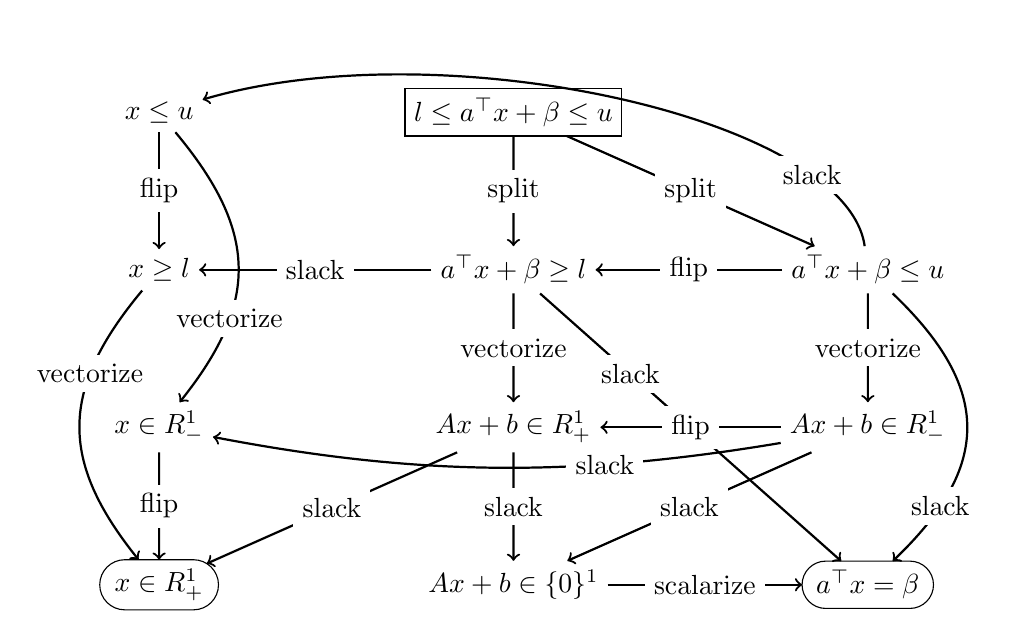
\begin{tikzpicture}[xscale=4.5, yscale=2]
      \tikzset{VertexStyle/.style = {}}
      \Vertex[x=1, y=-1, L={$a^\top x + \beta \ge l$}]{G}
      \Vertex[x=2, y=-1, L={$a^\top x + \beta \le u$}]{L}
      \Vertex[x=1, y=-2, L={$A x + b \in \mathbb{R}_+^1$}]{N}
      \Vertex[x=2, y=-2, L={$A x + b \in \mathbb{R}_-^1$}]{P}
      \Vertex[x=1, y=-3, L={$A x + b \in \{0\}^1$}]{Z}
      \Vertex[x=0, y=0, L={$x \le u$}]{VL}
      \Vertex[x=0, y=-1, L={$x \ge l$}]{VG}
      \Vertex[x=0, y=-2, L={$x \in \mathbb{R}_-^1$}]{VP}
      \tikzset{VertexStyle/.style = {
        shape = rectangle,
        draw
      }}
      \Vertex[x=1, y=0, L={$l \le a^\top x + \beta \le u$}]{I}
      \tikzset{VertexStyle/.style = {
        shape = rounded rectangle,
        draw
      }}
      \Vertex[x=2, y=-3, L={$a^\top x = \beta$}]{E}
      \Vertex[x=0, y=-3, L={$x \in \mathbb{R}_+^1$}]{VN}
      \tikzset{EdgeStyle/.style = {->}}
      \Edge[label={flip}](L)(G)
      \Edge[label={flip}](VP)(VN)
      \Edge[label={flip}](VL)(VG)
      \Edge[label={split}](I)(L)
      \Edge[label={split}](I)(G)
      \Edge[label={vectorize}](G)(N)
      \Edge[label={vectorize}](L)(P)
      \Edge[label={scalarize}](Z)(E)
      \Edge[label={slack}](P)(Z)
      \Edge[label={slack}](N)(Z)
      \Edge[label={slack}](N)(VN)
      \Edge[label={slack}](G)(VG)
      \tikzset{EdgeStyle/.style = {->, pos=0.3}}
      \Edge[label={slack}](G)(E)
      \tikzset{EdgeStyle/.style = {->, bend left=22, pos=0.3}}
      \Edge[label={slack}](P)(VP)
      \tikzset{EdgeStyle/.style = {->, bend left=20, pos=0.7}}
      \Edge[label={vectorize}](VL)(VP)
      \tikzset{EdgeStyle/.style = {->, bend left=25, pos=0.8}}
      \Edge[label={slack}](L)(E)
      \tikzset{EdgeStyle/.style = {->, bend right=20, pos=0.3}}
      \Edge[label={vectorize}](VG)(VN)
      \tikzset{EdgeStyle/.style = {->, bend right=25}}
      \tikzset{EdgeStyle/.style = {->, bend right=60, pos=0.2}}
      \Edge[label={slack}](L)(VL)
      \tikzset{EdgeStyle/.style = {->}}
      \Edge[label={flip}](P)(N)
    \end{tikzpicture}
    \caption{Bridging interval constraints to the linear programming standard form. The nodes in the form $x \in S$ represent constrained variables in $S$. The other nodes represent constraints.
    The interval constraint is surrounded by a sharp rectangle and the supported constrained variables and constraints are surrounded by a rectangle with rounded corners.
    The hyperedges are represented by multiple edges with the same label equal to the bridge name.
    The variable-to-constraint edges are omitted for clarity.}
    \label{fig:interval_bridges}
\end{figure}

\begin{figure}
    \centering
    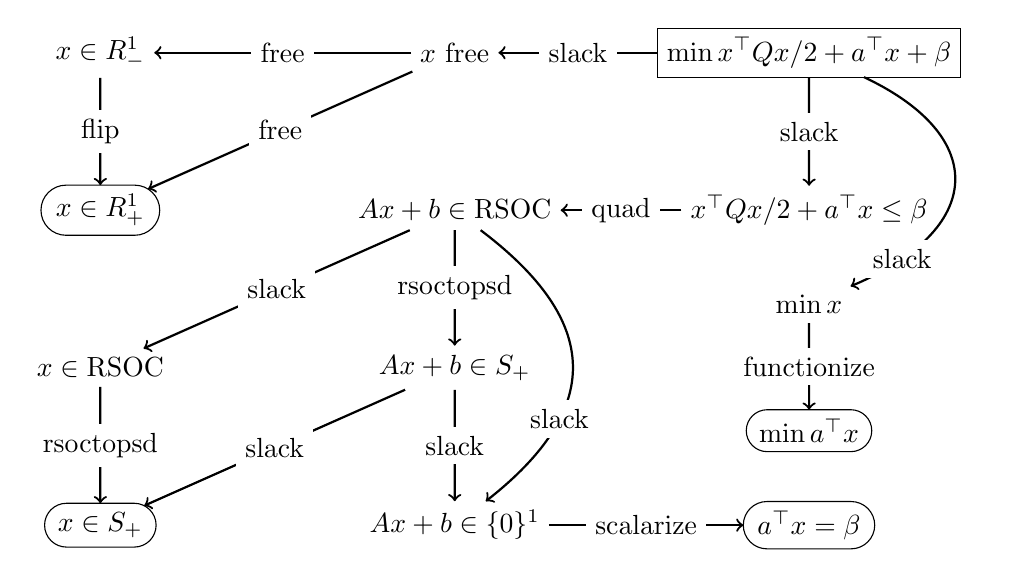
\begin{tikzpicture}[xscale=4.5, yscale=2]
      \tikzset{VertexStyle/.style = {}}
      \Vertex[x=2, y=-1, L={$x^\top Q x/2 + a^\top x \le \beta$}]{L}
      \Vertex[x=1, y=-1, L={$Ax + b \in {}$RSOC}]{R}
      \Vertex[x=1, y=-2, L={$A x + b \in \mathbb{S}_+$}]{P}
      \Vertex[x=0, y=-2, L={$x \in {}$RSOC}]{VR}
      \Vertex[x=1, y=-3, L={$A x + b \in \{0\}^1$}]{Z}
      \Vertex[x=1, y=0, L={$x$ free}]{F}
      \Vertex[x=0, y=0, L={$x \in \mathbb{R}_-^1$}]{VP}
      \Vertex[x=2, y=-1.6, L={$\min x$}]{SV}
      \tikzset{VertexStyle/.style = {
        shape = rectangle,
        draw
      }}
      \Vertex[x=2, y=0, L={$\min x^\top Q x/2 + a^\top x + \beta$}]{Q}
      \tikzset{VertexStyle/.style = {
        shape = rounded rectangle,
        draw
      }}
      \Vertex[x=2, y=-3, L={$a^\top x = \beta$}]{E}
      \Vertex[x=2, y=-2.4, L={$\min a^\top x$}]{AF}
      \Vertex[x=0, y=-3, L={$x \in \mathbb{S}_+$}]{VPSD}
      \Vertex[x=0, y=-1, L={$x \in \mathbb{R}_+^1$}]{VN}
      \tikzset{EdgeStyle/.style = {->}}
      \Edge[label={slack}](Q)(L)
      \Edge[label={slack}](Q)(F)
      \Edge[label={quad}](L)(R)
      \Edge[label={slack}](P)(Z)
      \Edge[label={slack}](P)(VPSD)
      \Edge[label={slack}](R)(VR)
      \Edge[label={scalarize}](Z)(E)
      \Edge[label={rsoctopsd}](R)(P)
      \Edge[label={rsoctopsd}](VR)(VPSD)
      \Edge[label={free}](F)(VP)
      \Edge[label={free}](F)(VN)
      \Edge[label={flip}](VP)(VN)
      \Edge[label={functionize}](SV)(AF)
      \tikzset{EdgeStyle/.style = {->, bend left=30, pos=0.7}}
      \Edge[label={slack}](R)(Z)
      \tikzset{EdgeStyle/.style = {->, bend left=45, pos=0.85}}
      \Edge[label={slack}](Q)(SV)
    \end{tikzpicture}
    \caption{Bridging quadratic objective to the semidefinite programming standard form. The nodes in the form $x \in S$ represent constrained variables in $S$. The nodes in the form min $f(x)$ represent objective function of the form $f(x)$. The other nodes represent constraints.
    The quadratic objective function is surrounded by a sharp rectangle and the supported constrained variables, constraints and objective functions are surrounded by a rectangle with rounded corners.
    The hyperedges are represented by multiple edges with the same label equal to the bridge name.
    The variable-to-constraint edges are omitted for clarity.}
    \label{fig:quadratic_bridges}
\end{figure}

We overcome the proliferation challenge by posing the question of how to transform one constrained variable, constraint or objective into supported equivalents as a shortest path problem through a graph.
The nodes in the graph represent either constrained variables in set, function-in-set pairs, or objective functions.
The transformation of a node into other nodes is represented by an edge with one source and multiple targets.
The number of edges representing the transformation of a given bridge is unlimited.
For instance, the slack bridge transforms any scalar $f(x) \in \mathcal{S}$ constraint into a constrained variable $s \in \mathcal{S}$ and a constraint $f(x) - s = 0$.
For any scalar function type \texttt{F} and scalar set type \texttt{S}, the slack bridge creates an edge from \texttt{F}-in-\texttt{S} to the two nodes \texttt{S} and \texttt{F}-in-$\{0\}$ (assuming that the type of the function $f(x) - s$ is also \texttt{F}).

\begin{myrem}
  \label{rem:jitbridges}
  Consider that implementation of bridges in Julia contained in MathOptInterface.
As the functions and sets considered is unlimited, the user can define new types in Julia even at run-time, representing the complete graph is out of the question.
For this reason, the computation of the shortest path is done in a \textit{just-in-time} fashion, so that we only compute the shortest path from a given node immediately prior to the first time a given constrained variable, function-in-set pair or objective function is added to a model.

Note the similarity with the just-in-time compilation of Julia methods. When a method is defined with abstract type, as the set of subtypes for a given abstract is not limited and new types can be added at run-time, Julia does not compile a method for any combination of concrete type but instead only compile a method for given concrete types once it is called with these types.
Of course, even if the set of subtypes was limited, compiling all the possible methods would not be very practical, and the same reasoning can be applied to bridges.
There is, however, an important distinction between Julia methods and bridges. When a function is called with given arguments types, the most specific method is selected through what is called \emph{multiple dispatch}.
However, when a given constraint is added with given function and set types, the bridges selected does not only depend on the function and set types but also on the solver being used through the shortest path algorithm that we present now.
\end{myrem}

Given a set of nodes $N$, a \emph{single source hyperedge} (also known as \emph{forward hyperarc}, e.g., in \cite{gallo1993directed}) $e = (s, T)$ has a source node $s \in N$ and target nodes $T \subseteq N$.
A \emph{directed hypergraph} $G(N, E)$ with single source hyperedges (also known as forward hypergraph, e.g., in \cite{gallo1993directed}) is represented by a set of nodes $N$ and a set of single source hyperedges $E \subseteq N \times \mathcal{P}(N)$.
The bridge graph can be represented as a directed hypergraph with single source hyperedges as follows.

There are three types of nodes in $N$:
one variable node for each set type \texttt{S} representing constrained variables in \texttt{S},
one constraint node for each pair of function type \texttt{F} and set type \texttt{S} representing \texttt{F}-in-\texttt{S} constraints and
one objective node for each type \texttt{F} representing objective function of type \texttt{F}.

For each variable node \texttt{S} and variable bridge that supports bridging constrained variables in \texttt{S},
there is a hyperedge with the variable node as source and all the nodes corresponding to all constrained variables and constraints added by the bridge as targets.
Similarly, for each constraint node \texttt{F}-in-\texttt{S} and constraint bridge that supports bridging constraints in \texttt{S},
there is a hyperedge with the constraint node as source and all the nodes corresponding to all constrained variables and constraints added by the bridge as targets.
At last, for each objective node \texttt{F} and objective bridge that supports bridging objective functions of type \texttt{F},
there is a hyperedge with the objective node as source and all the nodes corresponding to all constrained variables, constraints added and the objective function set by the bridge as targets.

In addition to these edges, corresponding to bridges, for each variable node corresponding to a scalar (resp. vector) set \texttt{S}, there is an hyperedge with the variable node as the source and as the target the constraint node
\texttt{F}-in-\texttt{S} where \texttt{F} is the type of a scalar variable (resp. the type of a vector of variables) if free variables are supported by the solvers and
\texttt{F} is the type of a scalar affine function (resp. the type of a vector affine function) otherwise.
This corresponds to constrained variables in \texttt{S} that are added as free variables that are then constrained with a \texttt{F}-in-\texttt{S} constraint.
If free variables are not supported by the solver, they are bridged hence the constraint will be force-bridged by the functionize bridge which is the reason the function type of the target is an affine function in this case.
We call these edges the variable-to-constraint edges.

Given a directed hypergraph $G(N, E)$ with single source hyperedges, a \emph{cycle} is a sequence of nodes and arcs $(v_1, e_1, \ldots, v_n, e_n, v_1)$ such that $e_i = (v_i, T_i)$ with $v_{i+1} \in T_i$.
A \emph{hyperpath} is a directed hypergraph $G'(N', E')$ such that
\begin{enumerate}
  \item $N' \subseteq N$, $E' \subseteq E$,
  \item or each $(s, T) \in E'$, $s \in N'$ and $T \subseteq E'$ and
  \item there is no cycle in $G'$.
\end{enumerate}

Given an unsupported variable, constraint or objective, a possible transformation into supported variables, constraints and objective can be represented by a minimal hyperpath starting at the corresponding node and ending at supported nodes.
Therefore, the search for a suitable model transformation can be formulated as a search for a hyperpath.
Moreover, this search can be guided by a chosen weighting function assigning a weight to hyperpaths.

The choice of weighting function has a significant impact both on the optimal hyperpath and on the computational tractability of the shortest hyperpath problem.
Indeed, if the weighting function is chosen to be the number of different bridges used, the shortest path problem is NP-complete \cite{italiano1989online}.
In the present case, if a bridge is used twice, it makes sense to include its weight twice as well so a more appropriate weight function is the number of bridges used with multiplicity.
This weighting function is part of the more general family of \emph{additive weighting functions} for which the shortest hyperpath problem can be solved efficiently with a generalization of Bellman-Ford or Dijkstra algorithms; see \cite[Section~6]{gallo1993directed} for more details.

In order to accommodate with the just-in-time nature of the approach,
we start with an empty hypergraph $G^*(N^*, E^*)$.
When the shortest hyperpath is required from a given nodes, the subpart of the hypergraph $G$ reachable from the node that is not yet in the hypergraph $G^*$.
Then we compute the shortest hyperpath from all new nodes.



\section{Semidefinite programming}
\label{sec:sdp}



For semidefinite programming, the standard conic form becomes:
\begin{equation}
  \label{eq:sdp_standard}
    \begin{array}{rl}
        \min\limits_{X \in \SymK[n]} & \la C, X \ra\\
        \text{subject to:} & \la A_i, X \ra = b_i, \quad i=1,2,\ldots,m\\
                           & X \succeq 0,
    \end{array}
\end{equation}
and the geometric conic form becomes
\begin{equation}
  \label{eq:sdp_conic}
    \begin{array}{rl}
        \max\limits_{y \in \mathbb{R}^m} & \la b, y \ra\\
        \text{subject to:} & C \succeq \sum_{i=1}^m A_i y_i\\
                           & y\ \mathsf{free},
    \end{array}
\end{equation}
where $C$ and $A_i$ are $n\times n$ symmetric matrices, $b_i$ is a constant scalar, $\langle \cdot, \cdot\rangle$ denotes the inner product, and $X \succeq 0$ enforces the matrix $X$ to be positive semidefinite.

The Lagrangian function of this pair of primal-dual program is given by
\begin{equation}
  \label{eq:LagrangianXy}
  L(X, y) = \la b, y \ra + \la C, X \ra - \sum_{i=1}^m \la y_i A_i, X \ra.
\end{equation}
Adding a slack variable $Z$, \eqref{eq:sdp_conic} is rewritten into
\begin{equation}
  \label{eq:sdp_conic_Z}
    \begin{array}{rl}
        \max\limits_{y \in \mathbb{R}^m} & \la b, y \ra\\
        \text{subject to:} & Z + \sum_{i=1}^M A_i y_i = C\\
                           & y\ \mathsf{free},\\
                           & Z \succeq 0.
    \end{array}
\end{equation}
The corresponding Lagrangian function becomes
\begin{equation}
  \label{eq:LagrangianXyZ}
  L(X, y, Z) = \la b, y \ra + \la Z, X \ra.
\end{equation}

The logarithmic barrier function associated to \eqref{eq:LagrangianXy} (resp. \eqref{eq:LagrangianXyZ}) is given by $L(X, y) - \mu \ln \det(X)$ (resp. $L(X, y, Z) + \mu \ln \det(Z)$).
In either cases, the KKT conditions are given by the primal and dual feasibility constraints
in addition to
\begin{equation}
  \label{eq:XYmu}
  X Z = \mu I.
\end{equation}
The optimal solutions $\opt{X}(\mu), \opt{y}(\mu), \opt{Z}(\mu)$ for different
values of $\mu$ form the \emph{central path}.
In the limit $\mu \to \infty$, the optimal solution, called the \emph{analytic center}, does not take
the objective function of \eqref{eq:sdp_standard} or \eqref{eq:sdp_conic} into account.
Starting from the analytic center, a path-following scheme can be used
to follow the central path for decreasing $\mu$.
The parameter $\mu$ is decreased step by step and at each step,
the value of $\opt{X}(\mu^+)$ for the next parameter $\mu^+$ is approximated from the approximated value
of $\opt{X}(\mu)$ for the previous parameter $\mu$ using the Newton method,
similarly to the homotopy continuation path-following scheme described in \secref{solvealg}.

More precisely, at each iteration, the current value of $\mu$ is estimated with
$\la X, Y \ra / n$, which comes from \eqref{eq:XYmu}.
Then, the target value of $\mu$ for the iteration is obtained as $\sigma \la X, Y \ra / n$
where $\sigma$ is the \emph{centering parameter}.
Directions $(\Delta X, \Delta y, \Delta Z)$ are then chosen so that
$(X + \Delta X, y + \Delta y, Z + \Delta Z)$ satisfies the primal and dual feasibility constraints and
satisfy a linear constraint on $\Delta X, \Delta y, \Delta Z$ based on the
nonlinear equation \eqref{eq:XYmu}.
Many different linearizations of this equation have been explored in the literature with
guarantees on the number of iterations ranging from $\sqrt{n} \ln \varepsilon$ to $n^{3/2} \ln \varepsilon$ to reduce the duality gap $\la X, Y \ra$ by a factor of $\varepsilon^{-1}$;
see \cite{monteiro2000path} for details.
The complexity of each iteration is however the same for each linearization approach
and is given by $\bigoh(mn^3 + m^2n^2 + m^3)$; see \cite{monteiro1999implementation}.
Assuming that $m \le n(n+1)/2$ (otherwise, the system $Ax = b$ simply has redundant rows that can be removed as a presolve step),
the complexity of each iteration is simplified to $\bigoh(mn^3 + m^2n^2)$.
Therefore, the overall complexity of decreasing the duality gap of a semidefinite program
by a factor of $\varepsilon^{-1}$ is given by
\begin{equation}
  \label{eq:sdp_complexity}
  \bigoh\big((mn + m^2)n^{5/2}\log(\varepsilon)\big).
\end{equation}

This primal-dual path-following method is implemented in various
solvers such as
    CSDP~\cite{borchers1999csdp}, %
    DSDP~\cite{dsdp1}, %
    MOSEK~\cite{mosek2017mosek81082},
    SDPA~\cite{yamashita2003implementation}, %
    SDPT3~\cite{tutuncu2003solving} or %
    SeDuMi~\cite{sturm1999using}. %
Alternatively, the semidefinite program can be solved using
a first-order operator-splitting method such as
\begin{itemize}
  \item the \emph{Newton conjugate gradient} (Newton-CG) like SDPNAL~\cite{yang2015sdpnal},
  \item the \emph{alternating direction method of multipliers} (ADMM) like CDCS~\cite{zheng2020chordal}, COSMO~\cite{garstka_2019} or SCS~\cite{ocpb:16} or
  \item the \emph{primal-dual hybrid gradient} (PDHG)~\cite{chambolle2011first} like ProxSDP~\cite{souto2018exploiting};
\end{itemize}

The first-order methods typically have a smaller memory footprint, as the Hessian is not computed,
and faster iteration.
On the other hand, second-order methods usually require fewer iterations
and can provide more accurate solutions.

\begin{myrem}
  \label{rem:sdpvol}
  Note that when minimizing the volume of an ellipsoid $\mathcal{E}_Q$ with $Q \in \SymK$,
  the value $-\ln(\det(Q))$ should be minimized by \propref{detell}.
  The interior-point method can be adapted by using the term $\ln \det Q$ instead of $\mu \ln \det Q$ in the objective.
  To the best of our knowledge, despite the apparently simple change, in practice, only
  SDPT3~\cite{tutuncu2003solving} have the feature of adding $\ln(\det(Q))$ in the objective function for
  a positive semidefinite matrix $Q$.
  For other solvers than SDPT3, the $\ln(\det(Q))$ objective can be reformulated
  as a $(2n) \times (2n)$ LMI and a power cone constraint or exponental cone constraints; see \cite[p.~149]{ben2001lectures}.
  For a solver not supporting these cones, the objective $\sqrt[n]{\det(Q)}$
  should be used instead as it can be reformulated
  as a $(2n) \times (2n)$ LMI and rotated second-order cone constraints; see \cite[p.~149]{ben2001lectures}.
\end{myrem}

\begin{myrem}
  \label{rem:psdsize}
  As the number of entries in a symmetric matrix grows quadratically with its size,
  positive semidefinite programs performs better with many PSD variables or LMI constraints
  of small size than with few of large size. %
\end{myrem}

Note that in the standard conic form, the solver does not support free variables.
Solvers such as CDCS~\cite{zheng2020chordal}, COSMO~\cite{garstka_2019}, MOSEK~\cite{mosek2017mosek81082}, SCS~\cite{ocpb:16}, SDPT3~\cite{tutuncu2003solving} or SeDuMi~\cite{sturm1999using} %
also support free variables but not CSDP~\cite{borchers1999csdp}, DSDP~\cite{dsdp1}, SDPA~\cite{yamashita2003implementation}, or SDPNAL~\cite{yang2015sdpnal}.
The following bridge is used in MathOptInterface~\cite{legat2021mathoptinterface} for solvers not supporting free variables.
\begin{myexem}
  As $\R =
  \begin{bmatrix}
    1 & -1
  \end{bmatrix} \R_+^2$,
  we can define a variable bridge from $\R$ to $\R_+^2$ by substituting
  the free variable $x$ for $y - z$ where $y, z \in \R_+$.
\end{myexem}

\begin{myexem}
  \label{exem:rsoc_to_psd}
  We can define variable and constraint bridges from the rotated second-order cone to the positive semidefinite cone using the linear transformation mapping the vector $(t, u, x)$
  to the matrix
  \[
    \begin{pmatrix}
      t & x^\Tr\\
      x & 2uI
    \end{pmatrix}.
  \]

  Indeed by \propref{schurcomp}, the matrix is positive definite if and only if
  \begin{align*}
    uI & \succ 0\\
    t - x^\Tr (2uI)^{-1} x & \succ 0
  \end{align*}
  which is equivalent to
  \begin{align*}
    u & > 0\\
    2tu & > x^\top x.
  \end{align*}

  Similarly, variable and constraint bridges from the second-order cone to the positive
  semidefinite cone can be defined using the linear
  transformation mapping the vector $(t, x)$ to the matrix
  \[
    \begin{pmatrix}
      t & x^\Tr\\
      x & tI
    \end{pmatrix}.
  \]
  Note, however, that if $x \in \R^n$, that gives a positive semidefinite
  constraint of dimension $n + 1$ while combining the bridge from second-order cone to the rotated second-order cone defined in \exemref{rsoc}
  with the bridge from rotated second-order cone gives a positive semidefinite matrix of dimension $n$.
  Therefore, in view of \remref{psdsize}, the bridge from the second-order cone to
  the positive semidefinite cone is not recommended, it should be replaced by the combination just mentioned.
  For instance, it is defined in MathOptInterface~\cite{legat2021mathoptinterface} but is not enabled by default.
\end{myexem}




\section{Sum-of-Squares programming}
\label{sec:sosprog}

Deciding whether a multivariate polynomial of degree $2d \geq 4$ is nonnegative is known to be co-NP-hard.
However a sufficient condition for a polynomial to be nonnegative is easy to check.
If a polynomial is SOS, see \defref{sos}, then it is obviously nonnegative.

It is well known that if $p(x)$ is a homogeneous polynomial of degree
$2d$ then each $q_k(x)$ must be an homogeneous polynomial of degree $d$;
this can be shown easily using the Newton polytope of $p(x)$ and
\cite[Theorem~1]{reznick1978extremal}.
We can check
whether a polynomial is SOS using semidefinite programming thanks to
the following theorem.
\begin{mytheo}[\cite{choi1995sums,nesterov2000squared,parrilo2000structured,parrilo2003semidefinite,shor1987class}]
  \label{theo:sos}
  A multivariate polynomial $p(x)$ is a sum-of-squares if and only if
  \[ p(x) = b^\Tr Q b \]
  where $Q$ is a symmetric positive semidefinite matrix and $b$ is a vector of polynomials.
\end{mytheo}

Given a polynomial basis $b$, let $C_b$ be the linear map from the coefficients of $Q$ to the coefficient of $p(x) = b^\Tr Q b$.
Given a vector of polynomials $b$ of length $N$, the cone $C_b \Psd[N]$ is a convex
cone of sum-of-squares polynomials.
It is not necessarily the cone of all sum-of-squares polynomials with these monomials though as shown in the following example:

\begin{myexem}
  \label{exem:newton}
  Any polynomial $p(x)$ such that the only terms of nonzero coefficient have monomials $x^4$, $x^2y^2$ or $y^4$
  can be expressed as $p(x) = b^\Tr Q b$ where $Q \in \SymK[2]$ and $b = (x^2, y^2)$.
  However, there does not exist any $Q \in \Psd[2]$ such that the sum-of-squares
  polynomial $2x^4 + 2x^2 y^2 = b^\Tr Q b$.
  This can be verified numerically as follows using \jlpkg{SumOfSquares} and CSDP~\cite{borchers1999csdp}.
\begin{minted}{Julia}
model = Model(CSDP.Optimizer)
@variable(model, p, SOSPoly([x^2, y^2]))
@constraint(model, p == 2x^4 + 2x^2 * y^2)
optimize!(model)
dual_status(model) # gives INFEASIBILITY_CERTIFICATE
\end{minted}
\end{myexem}

\begin{mydef}[Newton polytope]
  Given a polynomial $p(x)$, the convex hull of the set of exponents of the monomials of terms with nonzero coefficients of $p(x)$ is called the \emph{Newton polytope} of $p(x)$
  and is denoted $\mathcal{N}(p)$.
\end{mydef}

Given the Newton polytope of a polynomial $p(x)$,
the following result allows to determine a basis $b$ that contains
a sufficient set of monomials to make sure that $p(x)$ is a sum-of-squares
if and only if there exists a positive semidefinite matrix $Q$.

\begin{mytheo}[{\cite[Theorem~1]{reznick1978extremal}}]
  \label{theo:newton}
  If $p(x) = \sum_{k=1}^M q_k^2(x)$ then $2\mathcal{N}(q_k) \subseteq \mathcal{N}(p)$ for $k = 1, \ldots, M$.
\end{mytheo}

By \theoref{newton}, if the set of entries of the vector $b$ of length $N$ is the set of integer points of a polytope $\mathcal{P}$ then $C_b \Psd[N]$ is the set
of all sum-of-squares polynomials $p(x)$ such that $\mathcal{N}(p) \subseteq C_b \Psd[N]$.
This relation between the cone of sum-of-squares polynomials and positive semidefinite matrices is of the form~\eqref{eq:AS1S2} hence
it yields
\begin{itemize}
  \item a variable bridge from the cone of sum-of-squares polynomials
    to the cone of positive semidefinite matrices.
  \item a constraint bridge from the cone of positive semidefinite matrices
    to the cone of sum-of-squares polynomials.
\end{itemize}
The variable bridge is of tremendous practical importance as it allows to
solve SOS program with SDP solvers.
The constraint bridge could be useful as the dimension of the PSD cone
is larger than the dimension of the SOS cone when several entries of the matrix $bb^\Tr$
are equal.
However, it is not currently used in practice as there are no SOS solvers
that do not implement support for SDP constraints.

The constraint bridge from the cone of SOS polynomials to the cone of
positive semidefinite matrices is obtained by combining the slack bridge of \exemref{slack}
with the variable bridge from SOS polynomials to positive semidefinite matrices.

We denote the set of homogeneous polynomials of degree $2d$ as ${\Rh}[x]$.
\begin{mycoro}
  \label{coro:hsos}
  A homogeneous multivariate polynomial $p(x)$ of degree $2d$ is a sum
  of squares if and only if
  \[ p(x) = b^\Tr Q b \]
  where $Q$ is a symmetric positive semidefinite matrix
  and $b$ is a polynomial basis of ${\Rh[d]}[x]$.
\end{mycoro}

We denote the cone of homogeneous SOS polynomials of degree $2d$ as
$\Sosh$ and the dual of $\Sosh$ as $\Soshd$.
Note that the the dimension of $\Rh[d]$ is given by ${n+d-1 \choose d}$.
Therefore, verifying whether a homogeneous multivariate polynomial
of $n$ variables and degree $2d$ can be formulated as a semidefinite program~\eqref{eq:sdp_standard}
with a positive semidefinite variable $X$ of size ${n+d-1 \choose d} \times {n+d-1 \choose d}$.
Does the polynomial complexity of semidefinite programs given in \eqref{eq:sdp_complexity} imply that Sum-of-Squares program can be solved in polynomial time ?
As we have
\[
  {n+d-1 \choose d} = \frac{(n+d-1)!}{d!(n-1)!} = \frac{1}{d!} \prod_{i=n}^{n+d-1} i = \frac{1}{(n-1)!} \prod_{i=d+1}^{n+d-1} i,
\]
the binomial coefficient is both polynomial in $n$ for fixed $d$ and polynomial in $d$ for fixed $n$.
However, it is not a multivariate polynomial in both $n$ and $d$.
So the answer is affirmative if either $n$ or $d$ is fixed but is negative in terms of both $n$ and $d$.

From the exact arithmetic viewpoint, the basis $b$ chosen in \theoref{sos} does not affect whether $p(x)$ is SOS or not.
A specific choice of basis may, however, improve the numerical behavior of the corresponding semidefinite program.
Moreover considering a basis satisfying some
properties may facilitate the theoretical development.
For instance, in \lemref{sosbound}, we would need the basis $b = \ld{x}$ such that
$\enorm{\ld{x}} = \enorm{x}^d$.
This leads us to the choice of the \emph{scaled monomial} basis.
The elements of this basis are
\[ \frac{d!}{\alpha_1!\alpha_2!\cdots\alpha_n!} x_1^{\alpha_1} \cdots x_n^{\alpha_n}. \]
for each \ktups{n} of nonnegative integers $\alpha$ such that
$\alpha_1 + \cdots + \alpha_n = d$.
For any matrix $A \in \R^{n \times n}$, the $d$-lift induces an
associated map $A^{[d]} \in \R^{N_d \times N_d}$ which is the unique
matrix that satisfies $(Ax)^{[d]} = A^{[d]}x^{[d]}$.
We also have the following property for the standard inner product
between vectors
\begin{equation}
  \label{eq:liftscalprod}
  \la \ld{x}, \ld{y} \ra = (\la x, y \ra)^d.
\end{equation}

\subsection{Sum-of-Squares Convexity}
\label{sec:sosconv}
When considering polar polysets in \chapref{setprog}, we will need to constrain a polynomial to be convex.
This can be achieved by constraining its Hessian to be pointwise positive semidefinite.
The Hessian is a polynomial matrices, that is, a matrix with polynomial entries.
Thus the problem of checking convexity of a polynomial reduces to the problem of checking the pointwise positive semidefiniteness of a polynomial matrix.
Since polynomial nonnegativity is a special case of polynomial matrix positive semidefiniteness, the latter is also NP-hard.
Hence this reduction does not provide an efficient algorithm for polynomial convexity.

It turns out that checking the convexity or quasi-convexity of a multivariate polynomial is co-NP-hard even for quartic polynomials~\cite{ahmadi2013np}.
Thus checking whether the Hessian is positive semidefinite may actually be the best we can do.
We can define the generalization of SOS polynomial for polynomial matrices as follows.

\begin{mydef}[SOS matrices and SOS convexity]
  A symmetric polynomial matrix $P(x) \in \R[x]^{m \times m}$, $x \in \R^n$, is an \emph{SOS matrix} if there exists a polynomial matrix $M(x) \in \R[x]^{s \times m}$ for some $s \in \N$,
  such that $P(x) = M^\Tr(x)M(x)$.

  A polynomial $p(x)$ is \emph{SOS-convex} if its Hessian is an SOS matrix.
\end{mydef}

Polynomial matrix semidefiniteness is actually equivalent to polynomial nonnegativity.

\begin{mylem}
  Let $P(x) \in \R[s]^{m \times m}$ be a symmetric polynomial matrix,
  with $x \in \R^n$.
  Let $p(x,y) = y^T P(x) y$ be the associated scalar polynomial in $m+n$ variables where $y = [y_1, \ldots, y_m]$.
  \begin{enumerate}
    \item The matrix $P(x)$ is positive semidefinite if and only if $p(x,y)$ is nonnegative.
    \item The matrix $P(x)$ is an SOS matrix if and only if $p(x,y)$ is SOS (in $\R[x,y]$).
  \end{enumerate}
\end{mylem}

More information on SOS matrices can be found in \cite[Section~3.3.2]{blekherman2012semidefinite} and see \cite[Section~3.3.3]{blekherman2012semidefinite} or \cite{ahmadi2012convex,ahmadi2013complete} for sos convexity.
Sos convexity also plays a prominent role in certifying the stability of nonlinear switched systems~\cite{ahmadi2013switched,ahmadi2013sos}.

\subsection{Moments}
\label{sec:moments}

A common interpretation of the dual space $\Rhd$ of linear functionals on homogeneous polynomials of degree $2d$ is the space of moments of momonials of degree $2d$; see \cite[Section~3.5]{blekherman2012semidefinite} and \cite{Lasserre2009}.
If $p(x) = a^\Tr x^{[d]}$ and $m$ is the vector of moments of $x^{[d]}$ of a measure $\mu$ then
\[ \la m, a \ra = \int p(x) \dif \mu = \la \mu, p \ra. \]
As an SOS polynomial is nonnegative,
this integral is nonnegative for any measure $\mu$.
Therefore, given a moment vector $m$, a necessary condition for a measure to exist with these moments is that $\la m, a \ra \geq 0$ for any vector of coefficients $a$ of an SOS polynomial.
That is, $\Soshd$ is a superset of the set of moments of measures.
The members of $\Soshd$ are often called \emph{pseudo-measures} and denoted $\pmu$; see~\cite{barak2012hypercontractivity}.

Given a program on measures such as \progref{dualinf},
the \emph{moment relaxation} consists in truncating the infinite moment series to the finite
set of moments of the monomials in the matrix $M = bb^\Tr$ where $b$
is a finite polynomial basis.
The constraint that a measure exists with these moments is relaxed to a semidefinite
constraint on the moment matrix, defined in \defref{moment_matrix}, which is in fact equivalent to requiring that the measure belongs
to the cone $\Soshd$ introduced above.

\begin{mydef}[{\cite[Section~3.2.1]{Lasserre2009}}]
  \label{def:moment_matrix}
  Given a positive integer $d$ and a vector $y$ of moments of all the monomials
  up to degree $2d$, the \emph{moment matrix} is defined as the matrix $M_d(y)$,
  indexed by the exponents of monomials of degree $d$ such that
  $[M_d(y)]_{\alpha, \beta} = y_{\alpha + \beta}$ where $y_{\alpha + \beta}$ is
  the moment of the monomial $x^\alpha x^\beta$.
\end{mydef}

The following propositions shows that the membership of a point in an SOS-convex
polyset is SOS-representable.

\begin{myprop}[{\cite[Theorem~9]{helton2010semidefinite}}]
  \label{prop:sdprep}
  Given an SOS-convex polynomial $s(x) = \sum_\alpha s_\alpha x^\alpha$ of degree $2d$,
  the membership of the point $x$ to the set $\setbuild{x}{s(x) \le 0}$
  is equivalent to the existence of a vector $y$ of moments of all the monomials
  up to degree $2d$ such that $y_0 = 1$,
  such that the moment matrix $M_d(y)$, defined in \defref{moment_matrix},
  is positive semidefinite and $\sum_{\alpha} s_\alpha y_\alpha \le 0$.
\end{myprop}

\subsubsection{Atom extraction}
\label{sec:atom}

Given a positive semidefinite moment matrix $M$,
let $\mathcal{V}$ be the union of the support of any measure with the moment matrix $M$.
Given a measure $\mu$ and a nonnegative polynomial,
$\la \mu, p \ra = 0$ implies that $p$ is zero over the support of $\mu$.
Therefore, if $\la M, Q \ra = 0$ for a positive semidefinite matrix $Q$,
the SOS polynomial $b^\Tr Q b$ is zero over $\mathcal{V}$.
In particular, this is true for any rank one matrix $Q = q q^\Tr$ hence
we have $b^\Tr q = 0$ is zero over $\mathcal{V}$ of any for any vector $q$ such that $q^\Tr M q = 0$.
Let $M = UU^\Tr$ be the Cholesky decomposition, the variety $\mathcal{V}$ is contained in
the variety $V(I)$ where $I$ is the ideal generated by the polynomials $b^\Tr q$
where $Q$ is in the kernel of $U$.
When $V(I)$ is zero-dimensional, it means that any measure $\mu$ that has the moments $M$
is a sum of Dirac measures.

In practice, when $M$ is computed numerically, we use the kernel of its low-rank factorization instead~\cite{henrion2005detecting}.
The variety is verified to be zero-dimensional and the elements $a_i$ of $V(I)$ are computed as in \secref{solvealg}.
We can then find the weights $\lambda_i$ such that the moments of $\sum_i \lambda_i \delta_{a_i}$ are $M$ by solving a linear system of equations.

\begin{myexem}
  \label{exem:moment}
  Consider the following moment matrix of \cite[Section~4]{henrion2005detecting}:
\begin{minted}{Julia}
using DynamicPolynomials
@polyvar x y
using MultivariateMoments
μ = measure([1/9,     0,     1/9,     0, 1/9,   0,
               0,     0,       0,   1/3,   0, 1/3,
               0,     0,       1],
            [x^4, x^3*y, x^2*y^2, x*y^3, y^4, x^3,
           x^2*y, x*y^2,     y^3,   x^2, x*y, y^2,
               x,     y,       1])
ν = moment_matrix(μ, [1, x, y, x^2, x*y, y^2])
\end{minted}
  The variety $V(I)$, computed with a specific tolerance \texttt{ranktol}.
  The tolerance is used to transform the moment matrix into the variety $V(I)$ give the atoms.
  This transformation uses the SVD decomposition of the moment matrix and discards the polynomials of the generating basis of the ideal $I$ corresponding to a singular value lower than \texttt{ranktol}.
\begin{minted}{Julia}
MultivariateMoments.computesupport!(ν, 1e-16)
\end{minted}
  is $V(\la -y^2 + 1/3, -x^2 + 1/3 \ra)$.
  The elements of this variety are $(\pm 1/\sqrt{3}, \pm 1/\sqrt{3})$
  and the atomic measure obtained as:
\begin{minted}{Julia}
extractatoms(ν, 1e-16)
\end{minted}
  is
  \[
    \frac 14 \delta_{( 1/\sqrt{3},  1/\sqrt{3})} +
    \frac 14 \delta_{( 1/\sqrt{3}, -1/\sqrt{3})} +
    \frac 14 \delta_{(-1/\sqrt{3},  1/\sqrt{3})} +
    \frac 14 \delta_{(-1/\sqrt{3}, -1/\sqrt{3})}.
  \]
\end{myexem}

The classical application for this atom extraction is in polynomial optimization.
The minimization of a polynomial $p(x)$ over a basic semialgebraic
set $K$ can be rewritten as the maximization of $\gamma$
such that $p(x) - \gamma$ is nonnegative over $K$.
A hierarchy of sufficient conditions for this nonnegativity can be obtained with
\cororef{positiv} by increasing the degree considered in the polynomials of the certificate at each level of the hierarchy.
The dual of the constraint associated with this certificate of nonnegativity
is a matrix of moments $M$.
If this matrix is found be the moments of Dirac measures, it means that
the centers of the Diracs are minimizers and the value $\gamma$ is the
value of $p(x)$ at these minimizers.
We provide another application of atom extraction in \secref{certifylowerbound}.

\begin{myexem}
  \label{exem:atom}
Consider the polynomial optimization problem of
minimizing the polynomial $x^3 - x^2 + 2xy -y^2 + y^3$
over the polyhedron defined by the inequalities $x \ge 0, y \ge 0$ and $x + y \geq 1$.
The value of $p$ at $(1, 0)$, $(1/2, 1/2)$ and $(0, 1)$ are respectively $0$, $1/4$ and $0$:
\begin{minted}{Julia}
using DynamicPolynomials
@polyvar x y
p = x^3 - x^2 + 2x*y -y^2 + y^3
using SemialgebraicSets
S = @set x >= 0 && y >= 0 && x + y >= 1
p(x=>1, y=>0), p(x=>1//2, y=>1//2), p(x=>0, y=>1)
\end{minted}
As we will see below with Sum-of-Square Programming,
the optimal solutions are $(x, y) = (1, 0)$ and $(x, y) = (0, 1)$ with objective value $0$ but
Ipopt~\cite{biegler2009large} only finds the local minimum $(1/2, 1/2)$ with objective value $1/4$.
It is not surprising that Ipopt does not find the optimal solution,
as this solvers only ensures to find a locally optimal solution.
\begin{minted}{Julia}
using JuMP
using Ipopt
model = Model(Ipopt.Optimizer)
@variable(model, a >= 0)
@variable(model, b >= 0)
@constraint(model, a + b >= 1)
@NLobjective(model, Min, a^3 - a^2 + 2a*b -
                         b^2 + b^3)
optimize!(model)

@show termination_status(model)
@show value(a)
@show value(b)
@show objective_value(model)
\end{minted}
A Sum-of-Squares certificate that $p \ge \alpha$ over the domain \texttt{S}, ensures that $\alpha$ is a lower bound to the polynomial optimization problem.
The following program searches for the largest upper bound and finds zero.
\begin{minted}{Julia}
model = SOSModel(optimizer)
@variable(model, α)
@objective(model, Max, α)
@constraint(model, c3, p >= α, domain = S)

optimize!(model)
@show termination_status(model) # OPTIMAL
@show objective_value(model) # -2.0092711e-10
\end{minted}
Using the solution $(1/2, 1/2)$ found by Ipopt of objective value $1/4$
and this certificate of lower bound $0$ we know that the optimal objective value is in the interval $[0, 1/4]$
but we still do not know what it is (if we consider that we did not try the solutions $(1, 0)$ and $(0, 1)$ as done in the introduction).
If the dual of the constraint \texttt{c3} was atomic, its atoms would have given optimal solutions of objective value $0$ but that is not the case.
\begin{minted}{Julia}
using MultivariateMoments
ν3 = moment_matrix(c3)
extractatoms(ν3, 1e-3) # `nothing`
\end{minted}
When the variety $V(I)$ extracted from the moment matrix is not zero-dimensional,
\texttt{extractatoms} concludes that the measure is not atomic and return \texttt{nothing}.
In this case, we can verify as follows:
\begin{minted}{Julia}
ν3.support
\end{minted}
that the ideal $I$ we extract from the moment matrix is
$$\la x + y - 1 \ra$$
hence the dimension of $V(I)$ is 1.
This explains \texttt{extractatoms} returned \texttt{nothing}.

The constraint \texttt{c3} uses \propref{qmodule} to certify the
nonnegativity of $p - a$ over \texttt{S} with:
$$ p - \alpha = s_0 + s_1 x + s_2 y + s_3 (x + y - 1) $$
where $s_0, s_1, s_2, s_3$ are SOS.
By default, the basis of the SOS polynomials $s_i$ are chosen so that the degrees of $s_1 x$, $s_2 y$ and $s_3 (x + y - 1)$ match those of $p - \alpha$ and then
the basis of $s_0$ is selected using \theoref{newton} on the polynomial
$$ p - \alpha - s_1 x - s_2 y - s_3 (x + y - 1). $$

The maximum total degree (i.e. maximum sum of the exponents of $x$ and $y$) of the monomials of $p$ is 3 so the constraint in the program above is equivalent to \texttt{@constraint(model, p >= α, domain = S, maxdegree = 3)}.
That is, since $x$, $y$ and $x + y - 1$ have total degree 1, the SOS polynomials $s_1$, $s_2$ and $s_3$ have been chosen with maximum total degree $2$.
Since these polynomials are SOS, their degree must be even so the next maximum total degree to try is 4.
For this reason, the keywords \texttt{maxdegree = 4} and \texttt{maxdegree = 5} have the same effect in this example.
In general, if the polynomials in the domain are not all odds or all even, each value of \texttt{maxdegree} has different effect in the choice of the maximum total degree of $s_i$.
With \texttt{maxdegree} set to 5, the lower bound found is zero again.
\begin{minted}{Julia}
model = SOSModel(optimizer)
@variable(model, α)
@objective(model, Max, α)
@constraint(model, c5, p >= α, domain = S,
            maxdegree = 5)

optimize!(model)
@show termination_status(model) # OPTIMAL
@show objective_value(model) # 8.70000606e-8
\end{minted}
This time, the dual variable is atomic as it is the moments of the measure
$$0.5 \delta_{(1, 0)} + 0.5 \delta_{(0, 1)}.$$
Therefore the program provides both a certificate that $0$ is a lower bound and a certificate that it is also an upper bound since it is attained at the global minimizers $(1, 0)$ and $(0, 1)$.
\begin{minted}{Julia}
using MultivariateMoments
ν5 = moment_matrix(c5)
extractatoms(ν5, 1e-3)
\end{minted}
The ideal extracted from the moment matrix is
\[
  I = \la x + y - 1, y^2 - y, xy, x^2 + y - 1 \ra
\]
as obtained by:
\begin{minted}{Julia}
ν5 = moment_matrix(c5)
MultivariateMoments.computesupport!(ν5, 1e-3)
\end{minted}
We can compute the Gr\"{o}bner basis with:
\begin{minted}{Julia}
SemialgebraicSets.computegröbnerbasis!(
    ideal(ν5.support))
ν5.support
\end{minted}
which gives the Gr\"{o}bner basis:
\[
  I = \la x + y - 1, y^2 - y \ra.
\]
From which the solution $(1, 0)$ and $(0, 1)$ are as obtained
from the multiplication matrices as discussed in \secref{solvealg}.

\end{myexem}




\section{Parametrized program}
\label{sec:ddp}

We define in this section the concept of optimality and duality cuts that
is used in \secref{dirobj}, \secref{stochprog} and \secref{optientropic}.

Consider the function $f(p)$
defined as the optimal objective value of a conic program
parametrized by a vector of parameters $p$.
\begin{equation}\label{eq:conic_standard_form_param}
    \begin{array}{rl}
      f(p) = \min\limits_{x\in\mathbb{R}^N} & c^\top x\\
      \text{subject to:} & Ax = b - Cp\\
                         & x \in \mathcal{K},
    \end{array}
\end{equation}
If strong duality holds then this function can be equivalently
defined with the dual program where the convexity of $f(p)$ is apparent:
\begin{equation}\label{eq:conic_geometric_form_param}
  f(p) = \begin{array}{rl}
      \max\limits_{x\in\mathbb{R}^N} & \sprod{b}{y} - \msprod{C}{p}{y}\\
      \text{subject to:} & c - A^\Tr y \in \mathcal{K}^*\\
                         & y\ \mathsf{free}.
  \end{array}
\end{equation}

For a given value of the vector of parameters $p$, the
dual optimal solution $\opt{y}(p)$ provides a subgradient of $f$ at $p$ given
by the objective function of \eqref{eq:conic_geometric_form_param}:
$\sprod{b}{\opt{y}(p)} - \msprod{C}{p}{\opt{y}(p)}$ hence
\begin{equation}
  \label{eq:opticut}
  \forall \hat{p}, \quad \forall \hat{p}, f(\hat{p}) \ge \sprod{b}{\opt{y}(p)} - \msprod{C}{\hat{p}}{\opt{y}(p)}.
\end{equation}

Moreover, if \eqref{eq:conic_standard_form_param} is infeasible,
from any infeasibility ray $\opt{y}(p)$, by \propref{farkas},
we have $-C^\Tr \opt{y}(p) \in N_{\dom f}(p)$ hence
$f(p)$ is $+\infty$ over the halfspace
$\halfspace{C^\Tr \opt{y}(p)}{\sprod{b}{\opt{y}(p)}}$ and
\begin{equation}
  \label{eq:infcut}
  \dom(f) \subseteq \bigcap_{p} \halfspace{-C^\Tr \opt{y}(p)}{-\sprod{b}{\opt{y}(p)}}.
\end{equation}

Given the dual solution $\opt{y}(p)$ for different values of $p$,
\eqref{eq:opticut} and \eqref{eq:infcut} give
a polyhedral lower-approximation of the function $f$ as well as a polyhedron outer-approximation of its domain.
The affine lower approximation given by \eqref{eq:opticut} for each value of $p$
is called an \emph{optimality cuts}
and the halfspace given by \eqref{eq:infcut} for each value of $p$
is called a \emph{feasibility cuts}.

Starting from an initial lower approximation of $f(p)$,
we can iteratively minimize this lower approximation and then
refine it at the optimal solution $\opt{p}$ using \algoref{cutgen}.

\begin{algorithm}[!ht]
  \caption{Cut generation for a parametrized program.}
  \label{algo:cutgen}
  \begin{algorithmic}
    \STATE \textbf{Input} Value $p$ for the vector of parameters.
    \STATE Solve the pair of program \eqref{eq:conic_standard_form_param}/\eqref{eq:conic_geometric_form_param} with value $p$ for the vector of parameters.
    \IF{the program is infeasible}
    \STATE Get an infeasibility ray $\opt{y}(p)$ of \eqref{eq:conic_geometric_form_param}
    \STATE Intersect the domain of $f(p)$ with the feasibility cut given by the halfspace
    $\halfspace{-C^\Tr \opt{y}(p)}{-\sprod{b}{\opt{y}(p)}}$.
    \ELSE
    \STATE Get an feasible solution $y$ of \eqref{eq:conic_geometric_form_param}
    \STATE Intersect the graph of $f(p)$ with the optimality cut $f(p) \ge \sprod{b}{\opt{y}(p)} - \msprod{C}{\hat{p}}{\opt{y}(p)}$.
    \ENDIF
  \end{algorithmic}
\end{algorithm}







\implementations{\jlpkg{StructDualDynProg}.}

\chapter{Systems and control}
\label{chap:sys}

In this chapter, we define the different types of systems considered in this thesis.
In \secref{hybrid}, we define specific classes of hybrid systems with examples used throughout the text.
In \secref{auton}, we review the stability of the classes of autonomous systems and in \secref{control}
we detail the stabilizability of system with a continuous control input.

A system is defined either in continuous or discrete time.
The discrete-time systems often originates from the discretization of continuous-time systems
due to digitalization.
A continuous-time linear system is defined by the iteration
\begin{equation}
  \label{eq:contautonsys}
  \dot{x}(t) = A x(t), x(t) \in \mathcal{X}
\end{equation}
where $A \in \mathbb{R}^{n \times n}$ and $\mathcal{X} \subseteq \R^n$.

A discrete-time linear system is defined by the iteration
\begin{equation}
  \label{eq:discautonsys}
  x_k = A x_{k-1}, x \in \mathcal{X}
\end{equation}
where $A \in \mathbb{R}^{n \times n}$ and $\mathcal{X} \subseteq \R^n$.

\begin{mydef}[Invariant set]
  \label{def:autoninv}
  A set $S$ is \emph{invariant} for system \eqref{eq:contautonsys} (resp. \eqref{eq:discautonsys})
  if for any state $x_0 \in S$, the trajectory of the system with initial state $x_0$
  remains in $S$.
\end{mydef}

To represent uncertainty due to the imperfection of the model or actual randomness in the system being modeled,
a disturbance is added to the system:
\begin{align}
  \label{eq:contdisturbsys}
  \dot{x}(t) = A x(t) + C w(t), x(t) \in \mathcal{X}, w(t) \in \mathcal{W}\\
  \label{eq:discdisturbsys}
  x_k = A x_{k-1} + C w_{k-1}, x_k \in \mathcal{X}, w_k \in \mathcal{W}
\end{align}
where $A \in \R^{n_x \times n_x}, C \in \R^{n_x \times n_w}$.

We sometimes have a way to impact the state space $x$ of the system.
This is modeled using a control input $u$:
\begin{align}
  \label{eq:contcontrolsys}
  \dot{x}(t) = A x(t) + B u(t), x(t) \in \mathcal{X}, u(t) \in \mathcal{U}\\
  \label{eq:disccontrolsys}
  x_k = A x_{k-1} + B u_{k-1}, x_k \in \mathcal{X}, u_k \in \mathcal{U}
\end{align}
where $A \in \R^{n_x \times n_x}, B \in \R^{n_x \times n_u}$.



We will see that there is a strong relation between these systems and both disturbance algebraic systems:
\begin{align}
  \label{eq:contdisturbalgsys}
  D\dot{x}(t) & = A x(t), x(t) \in \mathcal{X}\\
  \label{eq:discdisturbalgsys}
  Dx_k & = A x_{k-1}, x_k \in \mathcal{X}
\end{align}
and control algebraic systems:
\begin{align}
  \label{eq:contcontrolalgsys}
  E\dot{x}(t) & = A x(t), x(t) \in \mathcal{X}\\
  \label{eq:disccontrolalgsys}
  Ex_k & = A x_{k-1}, x_k \in \mathcal{X}
\end{align}
where $D, E, A \in \R^{n \times r}$.
The integer $r$ is usually smaller than $n$ which gives a choice for $\dot{x}(t)$ or $x_k$.

\begin{mydef}[Robust invariant set]
  \label{def:robustinv}
  A set $S$ is \emph{robust invariant} for the system \eqref{eq:contdisturbsys} (resp. \eqref{eq:discdisturbsys}, \eqref{eq:contdisturbalgsys} or \eqref{eq:discdisturbalgsys})
  if for any state $x_0 \in S$, all trajectories of the system with initial state $x_0$ remain in $S$.
\end{mydef}

\begin{mydef}[Controlled invariant set]
  \label{def:controlinv}
  A set $S$ is \emph{controlled invariant} for system \eqref{eq:contcontrolsys} (resp. \eqref{eq:disccontrolsys}, \eqref{eq:contcontrolalgsys} or \eqref{eq:disccontrolalgsys})
  if for any state $x_0 \in S$, there exists a trajectory with initial state $x_0$ that remains in $S$.
\end{mydef}

\begin{myrem}
  \label{rem:disturbvscontrol}
  The difference between systems \eqref{eq:contdisturbsys}, \eqref{eq:discdisturbsys}
  and systems \eqref{eq:contcontrolsys}, \eqref{eq:disccontrolsys}
  is the nature of the external input $w$ or $u$.
  The disturbance $w$ has an adversarial nature, it is considered arbitrarily chosen in $\mathcal{W}$ and cannot be controlled.
  On the other hand, we can choose the control $u$ in $\mathcal{U}$ that fits our purpose.
  For this reason, the quantifier used in \defref{robustinv} is ``all'' while the quantifier
  used in \defref{controlinv} is ``exists''.
  A similar distinction applies for algebraic systems.
  For disturbance algebraic systems, the choice is arbitrary while for control algebraic systems,
  we can choose the vector $\dot{x}(t)$ or $x_{k}$ among all of them which have the same image through $E$.
\end{myrem}

The \emph{minimal invariant (convex) superset} of a set $\Sset$ is the intersection of all the invariant (convex) supersets of $\Sset$
and
the \emph{maximal invariant (convex) subset} of a set $\Sset$ is the union (resp. convex hull) of all the invariant (convex) subsets of $\Sset$.

The minimal (resp. maximal) invariant set is indeed an invariant set since the intersection (resp. union, convex hull) of invariant sets is invariant.


\implementations{\jlpkg{MathematicalSystems}.}

\section{Hybrid Systems}
\label{sec:hybrid}

In the previous section, the state space $\mathcal{X}$ considered is a subset of $\R^n$ which is usually convex.
However, there is an increasing need to model also a state $q$ that belongs to a small union of discrete values.
We refer to $x$ as the continuous part and $q$ as the discrete part of the state space.
A system with a purely continous state space is adequately modeled by one of the systems defined in the previous section.
A system with purely discrete state space can be modeled by an automaton.
\begin{mydef}
  \label{def:caut}
  We define the \emph{automaton} $\G(\Nodes, \Arcs)$
  as a directed and labelled strongly connected graph with \nodes{} $\Nodes$, \arcs{} $\Arcs$ and
  possibly with parallel \arcs{}
  such that no \node{} has zero ingoing or outgoing degree.
  Each \arc{} $(q, q', \sigma) \in \Arcs$ represents a transition from \node{} $q \in \node$ to \node{} $q' \in \Nodes$,
  where $\sigma \in [m]$ is the \emph{label}, corresponding to the transition.
\end{mydef}

When the state space has both a continuous and discrete part, we say that it is \emph{hybrid}.
Arguably the simplest model of hybrid system is the discrete-time s\witch{} linear system.
A discrete-time s\witch{} linear system is characterized by a finite set of matrices $\A \eqdef \{A_1, A_2, \ldots, A_m\} \subset \mathbb{R}^{n \times n}$ and the iteration
\begin{equation}
  \label{eq:switchsys}
  x_k = A_{\sigma_k} x_{k-1}, \quad \sigma_k \in [m]
\end{equation}
where $[m]$ denotes the set $\{1, \ldots, m\}$.

In some applications the values that $\sigma_k$ can take in \eqref{eq:switchsys} may depend on $\sigma_{k-1}, \sigma_{k-2}, \ldots$.
These constraints are often conveniently represented using a \emph{finite automaton} and the JSR under such constraints
is called \emph{constrained joint spectral radius} (CJSR) \cite{dai2012gel}; an example of constrained s\witch{} system is given by \exemref{run1} and its automaton is illustrated by \figref{run}.
Constrained switched systems are used in a variety of applications including
networked control \cite{brockett2000quantized, zhang2005new} and %
coordination of a network of autonomous agents \cite{jadbabaie2003coordination}. %
Moreover, even if a s\witch{} system is \emph{un}constrained,
studying an associated \emph{constrained} system generated by \emph{path-complete} methods
enhance our ability to analyze the stability~\cite{ahmadi2014joint}
or stabilize~\cite{gomes2018minimally} the original \emph{un}constrained switched system.

The following will serve as a running example of constrained s\witch{} system.

\begin{myexem}[Running example]%
  \label{exem:run1}
  We borrow the example of \cite[\Sect4]{philippe2016stability}.
  The set of matrices $\A$ is composed of the following four matrices
  \begin{align*}
    A_1 & = A+B
    \begin{pmatrix}
      k_1 & k_2
    \end{pmatrix},&
    A_2 & = A+B
    \begin{pmatrix}
      0 & k_2
    \end{pmatrix},\\
    A_3 & = A+B
    \begin{pmatrix}
      k_1 & 0
    \end{pmatrix},&
    A_4 & = A.
  \end{align*}
  where $k_1 = -0.49$, $k_2 = 0.27$,
  \[
    A =
    \begin{pmatrix}
      0.94 & 0.56\\
      0.14 & 0.46
    \end{pmatrix} \text{ and }
    B =
    \begin{pmatrix}
      0\\
      1
    \end{pmatrix}.
  \]

  The corresponding automaton is represented by Figure~\ref{fig:run}.

  \begin{figure}[!ht]
    \centering
    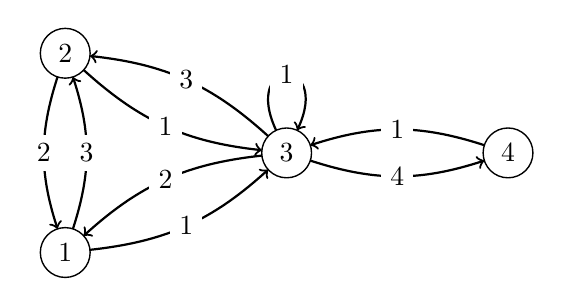
\begin{tikzpicture}[x=40,y=18]
       \Vertex{1}
       \NO[unit=4](1){2}
       \SOEA[unit=2](2){3}
       \EA[unit=2](3){4}
       \tikzset{EdgeStyle/.style = {->}}
       \tikzset{LoopStyle/.style = {->}}
       \tikzset{EdgeStyle/.append style = {bend right=18}}
       \Edge[label=1](1)(3)
       \Edge[label=3](1)(2)
       \Edge[label=2](2)(1)
       \Edge[label=1](2)(3)
       \Edge[label=2](3)(1)
       \Edge[label=3](3)(2)
       \Edge[label=4](3)(4)
       \draw[thick,->] (3) to [out=115,in=65,looseness=10] node [midway, fill=white] {1} (3);
       \Edge[label=1](4)(3)
     \end{tikzpicture}
     \caption{Automaton for the running example.
     The numbers on the \arcs{} are their respective labels.
     }
     \label{fig:run}
  \end{figure}
\end{myexem}

The iteration~\ref{eq:switchsys} is rewritten as follows to take the automaton into account:
\begin{equation}
  \label{eq:cswitchsys}
  x_k = A_{\sigma_k} x_{k-1}, \qquad (\sigma_1, \ldots, \sigma_k) \text{ are the respective labels of a path in }\G
  .
\end{equation}

The \emph{arbitrary switching} case~\eqref{eq:switchsys}
can be seen as the particular case when the automaton has only one node and $m$ self-loops with labels $1, \ldots, m$.

Note that \eqref{eq:cswitchsys} is not time-invariant as the value of $\sigma_k$ depends on previous values.
This resolved by adding the discrete part of the state space explicitly:
\begin{equation}
  \label{eq:cswitchsysq}
  x_k = A_{\sigma_k} x_{k-1}, \qquad
  (q_{k-1}, q_k, \sigma_k) \in \G.
\end{equation}







In general, the continuous part of the state space may exhibit both continuous-time and discrete-time dynamics.
In order to model such behavior, a common approach is to use \emph{\hsyss{}}.

\begin{mydef}[\Hsys{} \cite{alur1995algorithmic, johansson1999regularization}]
  \label{def:ha}
  A \emph{\hsys{}} is a collection
  $$(\G(\Nodes, \Arcs), \mathcal{X}, f, \Init, \Guard, R)$$
  where:
  \begin{itemize}
    \item $\G(\Nodes, \Arcs)$ is an automaton, as defined in \defref{caut}.
    \item $\mathcal{X}_q \subseteq \R^{n_q}$ is the state space constraint set for each \node{} $q$;
    \item $f_q$ is a time-invariant vector fields such that each $f_{q}(x)$
      is Lipschitz continuous on $\mathcal{X}_q$ for each \node{} $q$;
    \item $\Guard_\sigma$ defines a guard set for each transition. %
    \item $R_\sigma \in \mathcal{X}_{q'}$ specifies how the continuous state is reset for a transition
      $(q, q', \sigma) \in \Arcs$.
  \end{itemize}
  A trajectory of the system is a piecewise continuous trajectory $x(t)$, a sequence $(q_k)_k \in \Nodes$
  and a strictly increasing sequence $(t_k)_k$ such that for all $k$, we have
  \begin{align*}
    \dot{x}(t) & = f_{q_{k-1}}(x(t)), \quad x(t) \in \mathcal{X}_{q_{k-1}}, \quad t_{k-1} < t < t_k,\\
    x(t_k^+) & = R_{\sigma_k}(x(t_k^-)), \quad x(t_k^-) \in \Guard_{\sigma_k}\\
    (q_{k-1}, q_k, \sigma_k) & \in \G.
  \end{align*}
\end{mydef}

We allow the state space of different \nodes{} to differ by having different dimensions $n_q$ as our analysis naturally
extends to different state spaces but the reader may consider them to have identical dimension for simplicity.

When $\Guard_\sigma(x) \neq \R^{n_q}$, the switching is called \emph{state-dependent}.
When $\mathcal{X}_q, \Guard_\sigma$ are symmetric and $f_q, R_\sigma$ are homogeneous for each \node{} $q \in \Nodes$ and \signal{} $\sigma \in [m]$, we say that the \hsys{} is \emph{homogeneous}.

The constrained switched system \eqref{eq:cswitchsysq} is a special case of \hsys{}
where $\mathcal{X}_q = \R^n$ and $f_q(x) = 0$ (no continuous-time dynamics) for each $q \in \Nodes$,
$\Guard_\sigma(x) = \R^n$ (the switching is not state-dependent), and $R_\sigma(x) = A_\sigma$.

Another variant\footnote{This is not strictly a subclass of hybrid automaton since we add a control input.} of hybrid automaton we consider in this thesis is the class
of Discrete-Time Affine Hybrid Control System.
Similarly to constrained switched systems, these systems also do not have any continuous dynamic and the switching also not state-dependent.

\begin{mydef}
  \label{def:dtahcs}
  A \emph{Discrete-Time Affine Hybrid Control System (\dtahcs{})} is a system
  $\sys = (T,
           (A_\sigma, B_\sigma, c_\sigma)_{\sigma \in \Sigma},
           (\Ps_q, U_q)_{q \in \Nodes})$
  where $T = (\Nodes, \Sigma, \tr)$,
  $\Nodes$ is a finite set of \nodes{},
  $\Sigma$ is a finite set of \signals{} and
  $\tr \subseteq \Nodes \times \Sigma \times \Nodes$ is a set of transitions.
  We denote $(q, \sigma, q') \in \tr$ by $q \trs[\sigma] q'$.

  Given a \node{} $q \in \Nodes{}$, we denote
  the state dimension as $n_{q,x}$ and the input dimension as $n_{q,u}$.
  The set $\Ps_q \subseteq \mathbb{R}^{n_{q,x}}$ is the \emph{safe set}
  corresponding to \node{} $q$ and
  the set $U_q \subseteq \mathbb{R}^{n_{q,u}}$ is the set of allowed inputs.
  For any transition $q \trs[\sigma] q'$, we have
  $A_\sigma \in \mathbb{R}^{n_{q',x} \times n_{q,x}}$,
  $B_\sigma \in \mathbb{R}^{n_{q',x} \times n_{q,u}}$ and
  $c_\sigma \in \mathbb{R}^{n_{q',x}}$.

  A trajectory of $S$ is a sequence $\{(x_k,u_k,\sigma_k)\}_{k \in \mathbb{N}}$
  satisfying for all $k \in \mathbb{N}$:
  \begin{align*}
    x_{k+1} & = A_{\sigma_{k}} x_k + B_{\sigma_{k}} u_k + c_{\sigma_{k}},\\
    x_k \in \Ps_{q_k}, u_k &\in \U_{q_k}, q_k \trs[\sigma_{k}] q_{k+1}.
  \end{align*}
\end{mydef}

We say that the \dtahcs{} is homogeneous if $\Ps_q$ is symmetric for all $q \in \Nodes$ and $c_\sigma$ is zero for every \signal{} $\sigma$.

\begin{figure}[!h]
  \centering
  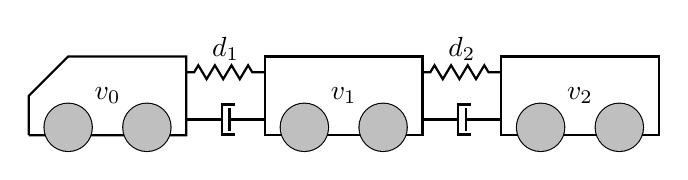
\begin{tikzpicture}
    \tikzstyle{spring}=[thick,decorate,decoration={zigzag,pre length=0.1cm,post length=0.1cm,segment length=6}]
\tikzstyle{damper}=[thick,decoration={markings,
  mark connection node=dmp,
  mark=at position 0.5 with
  {
    \node (dmp) [thick,inner sep=0pt,transform shape,rotate=-90,minimum width=10pt,minimum height=2pt,draw=none] {};
    \draw [thick] ($(dmp.north east)+(2pt,0)$) -- (dmp.south east) -- (dmp.south west) -- ($(dmp.north west)+(2pt,0)$);
    \draw [thick] ($(dmp.north)+(0,-4pt)$) -- ($(dmp.north)+(0,4pt)$);
  }
}, decorate]
\draw[thick] (0, 0) -- (2, 0) -- (2, 1) -- (0.5, 1) -- (0, 0.5) -- (0, 0);
\draw [spring] (2, 0.8) -- (3, 0.8);
\draw [damper] (2, 0.2) -- (3, 0.2);
\draw[thick] (3, 0) rectangle (5, 1);
\draw [spring] (5, 0.8) -- (6, 0.8);
\draw [damper] (5, 0.2) -- (6, 0.2);
\draw[thick] (6, 0) rectangle (8, 1);
\draw[thick] (0.5, 0.1) circle (0.3);
\fill[color=lightgray] (0.5, 0.1) circle (0.3);
\draw[thick] (1.5, 0.1) circle (0.3);
\fill[color=lightgray] (1.5, 0.1) circle (0.3);
\draw[thick] (3.5, 0.1) circle (0.3);
\fill[color=lightgray] (3.5, 0.1) circle (0.3);
\draw[thick] (4.5, 0.1) circle (0.3);
\fill[color=lightgray] (4.5, 0.1) circle (0.3);
\draw[thick] (6.5, 0.1) circle (0.3);
\fill[color=lightgray] (6.5, 0.1) circle (0.3);
\draw[thick] (7.5, 0.1) circle (0.3);
\fill[color=lightgray] (7.5, 0.1) circle (0.3);
\node at (1, 0.5) {$v_0$};
\node at (4, 0.5) {$v_1$};
\node at (7, 0.5) {$v_2$};
\node at (2.5, 1.1) {$d_1$};
\node at (5.5, 1.1) {$d_2$};

  \end{tikzpicture}
  \caption{Illustration for \exemref{cruise1} with two trailers.}
  \label{fig:cruise}
\end{figure}

We illustrate this definition with the cruise control example of \cite{rungger2013specification}.
\begin{myexem}[{see \cite[Section~6.1]{rungger2013specification}}]
  \label{exem:cruise1}
  We consider a truck with $M$ trailers as represented by \figref{cruise}.
  There is a truck with
  mass $m_0$ and
  speed $v_0$ followed by multiple trailers,
  each with mass $m$. The speed of the $i$th trailer is denoted $v_i$.
  There is a spring with stiffness $k_s$ and elongation $d_1$ (resp. $d_i$) and a damper with coefficient $k_d$
  between the truck and the first trailer (resp. the $(i-1)$th trailer and the $i$th trailer).
  The scalar input $u$ controls the speed $v_0$ of the truck
  by creating a force $m_0u$.
  The dynamics of the system is given by the following equations:
  \begin{align}
    \notag
    \dot{v}_0 & = \frac{k_d}{m_0}(v_1 - v_0) - \frac{k_s}{m_0} d_1 + u\\
    \notag
    \dot{v}_i & = \frac{k_d}{m}(v_{i-1} - 2v_i + v_{i+1}) + \frac{k_s}{m} (d_i - d_{i+1}) & 1 \leq i < M\\
    \label{eq:truckdyn}
    \dot{v}_M & = \frac{k_d}{m}(v_{M-1} - v_M) + \frac{k_s}{m} d_M\\
    \notag
    \dot{d}_i & = v_{i-1} - v_i & 1 \leq i \leq M.
  \end{align}
  The spring elongation should always remain between $-\SI{0.5}{\meter}$ and $\SI{0.5}{\meter}$ and the speeds of the truck and trailers should remain between $\SI{5}{\meter\per\second}$ and $\SI{35}{\meter\per\second}$.
  Moreover, there are three speed limits $\bar{v}_a = \SI{15.6}{\meter\per\second}$, $\bar{v}_b = \SI{24.5}{\meter\per\second}$, $\bar{v}_c = \SI{29.5}{\meter\per\second}$ and
  whenever the truck is informed of a new speed limit, it has \SI{0.8}{\second} to decrease $v_i$ ($0 \leq i \leq M$) below the speed limit.

  We sample time with a period of \SI{0.4}{\second} and define an initial \node{} $q_{d0}$ and 6 \nodes{} $q_{ij}$ where $i \in \{a, b, c\}$ is the current speed limitation and $j \in \{0, 1\}$ is the number of sampling times left to satisfy the limit.
  The transitions are $q_{ij} \trs[\sigma] q_{\sigma 1}$ for each $i \in \{a, b, c, d\}$ and $\sigma \in \{a, b, c, d\} \setminus \{i\}$.
  The \signal{} $a$ (resp. $b$, $c$) represents that the truck sees a new speed limitation $\bar{v}_a$ (resp. $\bar{v}_b$, $\bar{v}_c$) and $d$ represents that it does not see any new speed limitation.
  We suppose for simplicity that it is not possible to see a new speed limitation $\bar{v}_\sigma$ from a \node{} $q_{\sigma j}$.
  The possible transitions are represented in \figref{cruise1}.

  \begin{figure}[!ht]
    \centering
    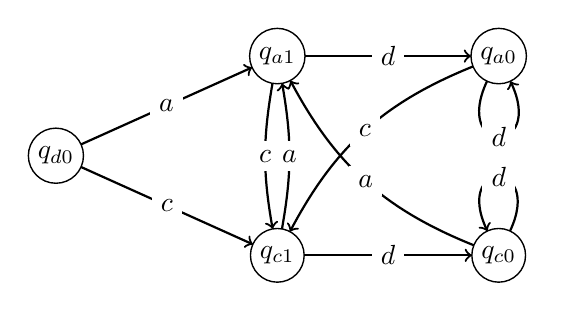
\begin{tikzpicture}[x=40,y=18]
      \Vertex[L={$q_{d0}$}]{0}
      \NOEA[unit=2,L={$q_{a1}$}](0){1}
      \EA[unit=2,L={$q_{a0}$}](1){2}
      \SOEA[unit=2,L={$q_{c1}$}](0){5}
      \EA[unit=2,L={$q_{c0}$}](5){6}
      \tikzset{EdgeStyle/.style = {->}}
      \tikzset{LoopStyle/.style = {->}}
      \Edge[label=$a$](0)(1)
      \Edge[label=$d$](1)(2)
      \Edge[label=$c$](0)(5)
      \Edge[label=$d$](5)(6)
      \tikzset{EdgeStyle/.append style = {bend right=20}}
      \Edge[label=$c$](2)(5)
      \tikzset{EdgeStyle/.append style = {bend right=-20}}
      \Edge[label=$a$](6)(1)
      \tikzset{EdgeStyle/.append style = {bend right=10}}
      \Edge[label=$c$](1)(5)
      \Edge[label=$a$](5)(1)
      \draw[thick,->] (2) to [out=-115,in=-65,looseness=9] node [midway, fill=white] {$d$} (2);
      \draw[thick,->] (6) to [out=65,in=115,looseness=9] node [midway, fill=white] {$d$} (6);
    \end{tikzpicture}
     \caption{Transitions and switchings between the \nodes{} for \exemref{cruise1}.
     Nodes $q_{b1}$ and $q_{b0}$ are not shown for clarity.
     }
     \label{fig:cruise1}
  \end{figure}


  The reset maps $(A_\sigma, B_\sigma, c_\sigma)$ are simply the integration of the dynamical system~\eqref{eq:truckdyn}
  over \SI{0.4}{\second} with a zero-order hold input extrapolation.

  Let
  \begin{align*}
    P_0 & = \{\, (d, v) \in \R^{2M+1} \mid -0.5 \leq d \leq 0.5, 5 \leq v \leq 35 \,\},\\
    P_i & = \{\, (d, v) \in \R^{2M+1} \mid v \leq \bar{v}_i \,\}, \quad i = a, b, c,
  \end{align*}
  where $d = (d_1, \ldots, d_M)$, $v = (v_0, \ldots, v_M)$ and inequalities in the two equations above are entrywise.
  The safe sets are $\Ps_{q_{d0}} = P_0$ and for $i = a, b, c$, $P_{q_{ij}} = P_0$ if $j > 0$ and $P_{q_{i0}} = P_0 \cap P_i$.
  The input set is $\U_{ij} = \{\, u \in \R \mid -4 \leq u \leq 4 \,\}$ for each \node{} $q_{ij}$.
\end{myexem}

Another variant of \hsys{} is given by Discrete-Time Affine Hybrid Algebraic Systems.

\begin{mydef}
  \label{def:dtahas}
  A \emph{Discrete-Time Affine Hybrid Algebraic System (\dtahas{})} is a system
  $\sys = (T,
           (A_\sigma, E_\sigma, c_\sigma)_{\sigma \in \Sigma},
           (\Ps_q)_{q \in \Nodes})$
  where $T = (\Nodes, \Sigma, \tr)$,
  $\Nodes$ is a finite set of \nodes{},
  $\Sigma$ is a finite set of \signals{} and
  $\tr \subseteq \Nodes \times \Sigma \times \Nodes$ is a set of transitions.

  Given a \node{} $q \in \Nodes{}$, we denote
  the state dimension as $n_{q,x}$.
  The set $\Ps_q \subseteq \mathbb{R}^{n_{q,x}}$ is the \emph{safe set}
  corresponding to \node{} $q$.
  For any transition $q \trs[\sigma] q'$, we have
  $A_\sigma \in \mathbb{R}^{n_{\sigma, p} \times n_{q, x}}$,
  $B_\sigma \in \mathbb{R}^{n_{\sigma, p} \times n_{q', x}}$ and
  $c_\sigma \in \mathbb{R}^{n_{\sigma, p}}$ for some natural number $n_{\sigma, p}$.

  A trajectory of $S$ is a sequence $\{(x_k,\sigma_k)\}_{k \in \mathbb{N}}$
  satisfying for all $k \in \mathbb{N}$:
  \begin{align*}
    E_{\sigma_{k}} x_{k+1} & = A_{\sigma_{k}} x_k + c_{\sigma_{k}},\\
    x_k & \in \Ps_{q_k}, q_k \trs[\sigma_{k}] q_{k+1}.
  \end{align*}
\end{mydef}

\begin{mydef}
  \label{def:homogeneous}
  We say that a \dtahas{} is \emph{homogeneous} if $P_q$ is symmetric for all $q \in \Nodes$ and $c_\sigma$ is zero for all \signal{} $\sigma$.
\end{mydef}





\section{Stability}
\label{sec:auton}

We review in this section classical approaches for computing
invariant ellipsoids and polysets for the systems defined above.

\subsection{Continuous-time systems}

The \emph{Nagumo condition} provides necessary and sufficient conditions
for invariance of continuous-time systems.
\begin{mytheo}[{Nagumo condition \cite[Theorem~4.7]{blanchini2015set}}]
  \label{theo:nagumo}
  A closed set $\mathcal{S}$ is invariant for system~\eqref{eq:contautonsys}
  if and only if
  \begin{equation}
    \label{eq:nagumo}
    \forall x \in \partial \mathcal{S}, Ax \in T_{\mathcal{S}}(x).
  \end{equation}
\end{mytheo}
For ellipsoids $\mathcal{E}_P$, the nagumo condition~\eqref{eq:nagumo} is rewritten as
\[ x^\Tr PAx \leq 0, \quad x \in \mathbb{R}^n. \]
which is equivalent to the LMI:
\begin{equation}
  \label{eq:cont_auton_LMI}
  A^\Tr P + PA \preceq 0.
\end{equation}
which allows to search for ellipsoidal invariant sets using
semidefinite programming.


\subsection{Discrete-time systems}

\label{sec:discsys}

Consider an ellipsoidal set $\mathcal{S} = \mathcal{E}_Q$, as defined in \eqref{eq:ell}.
Using \propref{gA}, the invariant condition of \defref{autoninv} for a discrete-time linear system \eqref{eq:discautonsys}
can be rewritten in terms of $Q$ as:
if $x^\Tr P x \leq 1$ then $x^\Tr A^\Tr P A x \leq 1$.
By the \propref{ellincl}, $x^\Tr P x \leq 1$ implies $x^\Tr A^\Tr P A x \leq 1$ if
and only if the following LMI holds:
\begin{equation}
  \label{eq:disc_auton_LMI}
  Q \succeq A^\Tr Q A.
\end{equation}


\subsubsection{Robust stability}

With the presence of a disturbance $w \in W = \mathcal{E}_Q$ in the system $x_{k+1} = Ax_k + Bw_k$, the condition becomes:
\begin{equation}
  \label{eq:forall}
  w^\Tr Q w \le 1, x^\Tr P x \le 1 \Rightarrow (A x + Bw)^\Tr P (A x + Bw) \le 1.
\end{equation}
and \propref{lossysproc} can be applied to provide a robust invariance LMI; see \cite[(6.5)]{boyd1994linear}.

\subsection{Discrete-time switched systems}
\label{sec:sosswitch}


The maximal asymptotic growth rate of \eqref{eq:switchsys} is given by the \emph{joint spectral radius} (JSR).
The JSR $\jsr$ of a finite set of matrices $\A$
is defined as
\[ \jsr = \lim_{k \to \infty} \max_{\sigma \in [m]^k} \|A_{\sigma_k} \cdots A_{\sigma_2} A_{\sigma_1}\|^{1/k}. \]
This definition is independent of the norm used.
The joint spectral radius is alternatively defined as the infimum value of $\sigma$ such that the monoid generated by the
matrices $A_1 / \sigma, \ldots, A_m / \sigma$ with the matrix product is bounded; see \defref{monoidgen}.

The JSR was introduced by Rota and Strang~\cite{rota1960note}
and has many other applications such as wavelets, the capacity of some particular codes, zero-order stability of ordinary differential equations, congestion control in computer networks, curve design and networked and delayed control systems; see \cite{jungers2009joint} for a survey on the JSR and its applications.
Many algorithms exist for estimating the JSR but not much is known on how to generate an infinite
sequence of matrices with an asymptotic growth rate close to the JSR.
However generating such sequence can be of particular interest, depending on the application,
such as exhibiting unstable trajectories for s\witch{} linear systems to prevent them from occuring~\cite{gomes2018minimally}. %
The currently known algorithms generate a sequence of matrices with high spectral radius
using methods detailed in \secref{lb}
and repeat this sequence infinitely \cite{gripenberg1996computing,guglielmi2008algorithm,guglielmi2013exact,jungers2014lifted}.

Approximating the JSR usually consists in certifying upper bounds $\gamub$ to the JSR by exhibiting a Lyapunov function or an invariant set for the matrices $A_i/\gamub$.
The search for such Lyapunov functions can naturally be written as a convex optimization program; see \progref{primalinf}.

The definition of the JSR is generalized as follows for constrained systems.
\begin{mydef}[\cite{dai2012gel}]
  \label{def:cjsr}
  The \emph{constrained joint spectral radius} (CJSR) of
  \defAG{}, denoted as $\cjsr$,
  is
  \begin{equation}
    \label{eq:jsrtheo}
    \limsup_{k \to \infty} \cjsrrk = \cjsr = \lim_{k \to \infty} \cjsrk
  \end{equation}
  where
  \begin{equation}
    \label{eq:cjsrrk}
    \cjsrrk
    = \max \big\{\, \jsrc : c \in \G_k, c \text{ is a cycle}\,\big\}, \quad \jsrc = [\rho(A_c)]^{1/k},
  \end{equation}
  and
  \begin{equation}
    \label{eq:cjsrk}
    \cjsrk =
    \max \big\{\, \|A_s\|^{1/k}\\: s \in \G_k \,\big\}.
  \end{equation}
\end{mydef}

We can readily see that
\(
  \cjsrrk \leq \cjsrk
\)
for any $k$ and \emph{submultiplicative}\footnote{A matrix norm $\norm{\cdot}$ is \emph{submultiplicative} if $\norm{AB} \leq \norm{A} \cdot \norm{B}$ for all matrices $A$ and $B$.} norm $\norm{\cdot}$.
Equality \eqref{eq:jsrtheo} is called the \emph{Joint Spectral Radius Theorem} and was proved in 1992 by Berger and Wang~\cite{berger1992bounded} in the unconstrained case.
Elsner~\cite{elsner1995generalized} provided a somewhat simpler self contained proof in 1995.
Both proofs use rather involved results on the joint spectral radius.
In the general constrained case, the equality \eqref{eq:jsrtheo}
was first proved in \cite{dai2012gel} with the help of heavy-weighted machinery
of ergodic theory, and later simpler proofs appeared.







\implementations{\jlpkg{SetProg}.}


Consider the space of bounded measurable
functions on $\Sn = \{\, x \in \R^n : \norm{x}_2 = 1 \,\}$, denoted $\Fb$, where $\norm{\cdot}_2$ is the \emph{Euclidean} norm.
Given a function $f(x) \in \Fb$, we can define the homogeneous\footnote{A function $f$ is homogeneous if $f(\alpha x) = \alpha f(x)$ for any scalar value $\alpha$.}
function $h(f) \eqdef x \mapsto \|x\|_2f(x/\|x\|_2)$ on $\R^n$.
We define
\begin{equation}
  \label{eq:homfun}
  \F = \{\, h(f) \mid f \in \Fb \,\}.
\end{equation}

Let $\Fp$ (resp. $\Fbp$) be the set of nonnegative functions of $\F$ (resp. $\Fb$)
and $\Fpp$ be the set of positive functions of $\F$.
Given two functions $f, g \in \F$, $f \geq 0$ denotes $f \in \Fp$ and $f \geq g$ denotes $f - g \in \Fp$.

\begin{myprog}[Primal]
  \label{prog:primalinf}

  \emph{Input}: A finite set of matrices $\A$ and an automaton $\G$.

  \emph{Output}: Functions $f_v$ and a number $\gamub$.
  \begin{align}
    \notag
    \inf_{f_v \in \F, \gamub \in \R} \gamub\\
    \label{eq:primalinf1}
    \text{subject to }f_v(A_\sigma x) & \leq \gamub f_u(x), \quad \forall x \in \R^n, \forall (u, v, \sigma) \in \Arcs,\\
    \notag
    f_v(x) & \in \Fpp, \quad \forall v \in \Nodes,\\
    \label{eq:primalinf3}
    \sum_{v \in V} \int_{\Sn} f_v(x) \dif x & = 1.
  \end{align}
\end{myprog}

\begin{mytheo}
  \label{theo:stabcert}
  Consider \defAGe{}.
  We have
  \( \lim_{k \to \infty} \cjsrk \leq \gamubopt. \)
  for the optimal solution $\gamubopt$ of \progref{primalinf}.
  \begin{proof}
    Consider a norm $\|\cdot\|$ of $\R^n$ and its corresponding induced matrix norm of $\R^{n \times n}$.
    For each $v \in \Nodes$, we know by compactness of the unit ball in $\R^n$, continuity and strict positivity of $f_v(x)$ that there exist $0 < \alpha_v \leq \beta_v$ such that
    \[ \alpha_v \|x\| \leq f_v(x) \leq \beta_v\|x\| \]
    for all $x \in \R^n$.
    Let $\alpha = \min_{v \in \Nodes} \alpha_v$ and $\beta = \max_{v \in \Nodes} \beta_v$.

    For a $\G$-admissible $k$-uple $(\sigma_1, \sigma_2, \ldots, \sigma_k)$,
    \( \|A_{\sigma_k} \cdots A_{\sigma_1}\| = \sup_{x \neq 0} \frac{\|A_{\sigma_k} \cdots A_{\sigma_1}x\|}{\|x\|}. \)
    Consider a path such that the $i$th edge has label $\sigma_i$ for $i = 1, \ldots, k$
    and denote the intermediary nodes of that path as $v_0, v_1, \ldots, v_k$.
    For any $x \in \R^n$, we have
    \begin{align*}
      \|A_{\sigma_k} \cdots A_{\sigma_1}x\| %
                                            \leq \alpha_{v_k} f_{v_k}(A_{\sigma_k} \cdots A_{\sigma_1} x)%
                                            \leq \alpha_{v_k} \gamub f_{v_{k-1}}(A_{\sigma_{k-1}} \cdots A_{\sigma_1} x)%
                                            \leq \alpha_{v_k} \gamub^{k} f_{v_0}(x)
    \end{align*}
    and
    \( \|x\| \geq \beta_{v_0} p_{v_0}(x) \)
    hence
    \( \|A_{\sigma_k} \cdots A_{\sigma_1}\| \leq \frac{\beta_{v_0}}{\alpha_{v_k}} \gamub^k \leq \frac{\beta}{\alpha} \gamub^k. \)
    Taking the $k$th root, the limit $k \to \infty$ and using \defref{cjsr} we obtain the result.
  \end{proof}
\end{mytheo}



The gauge function of polysets of degree $2d$ can be used as Lyapunov function.
\begin{mytheo}[\cite{parrilo2008approximation, philippe2016stability}]
  \label{prop:pos}
  Consider \defAGe{}.
  Suppose that there exist $|\Nodes|$ strictly positive homogeneous polynomials $p_v(x)$ of degree $2d$
  such that
  \[ p_{v}(A_\sigma x) \leq \gamub^{2d}p_{u}(x) \]
  holds for all \arc{} $(u,v,\sigma) \in \Arcs$.
  Then $\cjsr \leq \gamub$.
  \begin{proof}
    Define $f_v(x) = [p_v(x)]^{\frac{1}{2d}}$ and use \theoref{stabcert}.
  \end{proof}
\end{mytheo}

We relax the positivity condition of \propref{pos} by the more tractable sum-of-squares (SOS) condition and
define $\jsrsos$ as the solution of the following SOS restriction of \progref{primalinf}.
\begin{myprog}[Primal]

  \emph{Input}: A finite set of matrices $\A$ and an automaton $\G$.

  \emph{Output}: Polynomials $p_v(x)$ and a number $\gamub$.
  \label{prog:primal}
  \begin{align}
    \notag
    \inf_{p_v(x) \in \Rh[x],\gamub \in \R} \gamub\\
    \label{eq:soscons2}
    \text{subject to }\gamub^{2d} p_u(x) - p_v(A_\sigma x) & \text{ is SOS}, \quad \forall (u, v, \sigma) \in \Arcs,\\
    \label{eq:soscons1}
    p_v(x) & \text{ is SOS}, \quad \forall v \in \Nodes,\\
    \label{eq:soscons3}
    p_v(x) & \text{ is strictly positive}, \quad \forall v \in \Nodes,\\
    \notag
    \sum_{v \in V} \int_{\mathbb{S}^{n-1}} p_v(x) \dif x & = 1.
  \end{align}
\end{myprog}

\begin{myrem}
  In practice we can replace \eqref{eq:soscons1} and \eqref{eq:soscons3} by ``$p_v(x) - \epsilon\|x\|_2^{2d}$ is SOS''
  for any $\epsilon > 0$.
  This constrains $p_v(x)$ to be in the interior of the SOS cone,
  which is sufficient for $p_v(x)$ to be strictly positive.
  The bounds given in \Sect\ref{sec:quality} are valid
  if $p_v(x)$ is in the interior of the SOS cone.

\end{myrem}

By \propref{pos},
a feasible solution of Program~\ref{prog:primal} gives an upper bound for $\cjsr$,
and thus, for any positive degree $2d$,
\begin{equation}
  \label{eq:upperbound}
  \cjsr \leq \jsrsos.
\end{equation}


\begin{myexem}
  \label{exem:simple1}
  Consider the unconstrained system \cite[Example~2.1]{ahmadi2012joint} with $m=3$:
  \[ \A = \{ A_1 = e_1e_2^\Tr , A_2 = e_2e_3^\Tr , A_3 = e_3e_1^\Tr  \} \]
  where $e_i$ denotes the $i$th canonical basis vector.

  For any $d$, a solution to Program~\ref{prog:primal} is given by
  \[ (p(x), \gamma) = (x_1^{2d} + x_2^{2d} + x_3^{2d}, 1). \]
  Indeed, for example, with $A_1$ we have
  \[ p(e_1e_2^\Tr x) = p(x_2, 0, 0) = x_2^{2d} + 0 + 0 \leq x_1^{2d} + x_2^{2d} + x_3^{2d}. \]
\end{myexem}

\begin{myexem}
  \label{exem:run2}
  Let us reconsider our running example; see \exemref{run1}.
  The optimal solution of Program~\ref{prog:primal}
  is represented by
  Figure~\ref{fig:primal} for $2d = 2$ and 12.
  We can see a big difference between the shape of the sublevel sets
  for $2d = 2$ and $2d = 4$
  while between $2d=4$ and $2d=12$,
  the difference seems to be more subtle.
  \begin{figure}[!ht]
    \centering
    \tabulinesep=0.5mm
    \begin{tabu}{{X[0.85,c,m]X[c,m]X[c,m]X[c,m]X[c,m]}}
      & Node 1 & Node 2 & Node 3 & Node 4\\
      \PrimalFig{2}{1}
      \PrimalFig{4}{2}
      \PrimalFig{6}{3}
      \PrimalFig{8}{4}
      \PrimalFig{10}{5}
      \PrimalFig{12}{6}
    \end{tabu}
    \caption{
    Representation of the solutions to Program~\ref{prog:primal}
    with different values of $d$ for the running example.
    The blue curve represents the boundary of the
    polyset $\polyset[p_v]$ where $p_v$ is the optimal
    solution for each node $v \in \Nodes$.
    The dashed curve is the boundary of the unit circle.
    Observe that some sets are not convex.}
    \label{fig:primal}
  \end{figure}
\end{myexem}







\section{State feedback stabilitization}
\label{sec:control}

The problem of computing a controlled invariant set is a paradigmatic challenge in the broad field of Hybrid Systems control.
Indeed, it is for instance crucial in safety-critical applications,
such as the control of a platoon of vehicles or air traffic management; see \cite{tomlin1998conflict},
where firm guarantees are needed on our ability to maintain the state in a safe region
(e.g., with a certain minimal distance between vehicles).
In other situations, the dynamical system might be too complicated to analyze exactly in every point of the state space,
yet it can be possible to confine the state within a guaranteed set.
Such situations occur frequently in hybrid, embedded, event-triggered systems, because of the complexity of the dynamics.

A set is \emph{controlled invariant} (sometimes also referred to as \emph{viable})
if, any trajectory whose initial point is in the set can be kept inside it by means of a proper control action.
Given a system with constraint specifications on the states and/or input, the controlled invariant set can be used
to determine initial states such that trajectories with these initial conditions are guaranteed to meet the specifications.
Moreover, in some situations, a state feedback control law can be derived from the knowledge of the controlled invariant set; see \cite{blanchini1999survey} for a survey.

The existence of a controlled invariant set is equivalent to the stabilizability of a control system~\cite{sontag1983lyapunov}.
A (possibly nonlinear) stabilizable state feedback can be deduced from the controlled invariant set~\cite{barmish1985necessary}.

The stabilizability of a linear time-invariant (LTI) control system is equivalent
to the stability of its uncontrollable subspace (which is readily accessible
in its Controllability Form) \cite[Section~2.4]{wonham1974linear}.
Indeed, the eigenvalues of its controllable subspace can be fixed to any value
by a proper choice of linear state feedback.
The resulting controlled system is stable hence an invariant ellipsoid can be
determined by solving a system of linear equations~\cite{Liapounoff1907}.
This set is also controlled invariant for the control system.
When a control system admits an ellipsoidal controlled invariant set,
it is said to be \emph{quadratically stabilizable}.
When there exists a linear state feedback such that the resulting controlled
system admits an ellipsoidal invariant set, it is said to be
\emph{quadratically stabilizable via linear control}.

While the stabilizability of LTI control systems is equivalent to their
quadratic stabilizability via linear control,
it is no longer the case for \emph{uncertain} or \emph{switched} systems \cite{petersen1985quadratic}.
Furthermore, it is often desirable to find a controlled invariant set of maximal
volume (or which is maximal in some direction~\cite{ahmadi2018robust}).
For such problem, the method detailed above is not suitable as it does not
take any volume consideration but more importantly, the maximal volume
invariant set may not be an ellipsoid and may not be rendered stable via
a linear control.
For this reason, the Linear Matrix Inequality (LMI) \eqref{eq:cont_control_LMI} was devised to encapsulate the
controlled invariance of an ellipsoid via linear control \cite[Section~7.2.2]{boyd1994linear}
and the conservatism of the choice of linear control was analyzed \cite{sontag1983lyapunov}.
As the linearity of the control was found to be conservative for uncertain systems \cite{petersen1985quadratic},
the LMI \eqref{eq:invLMI} was found to encapsulate controlled invariance of an ellipsoid
via \emph{any} state-feedback \cite{barmish1985necessary}.

\subsection{Continuous-time systems}

With the presence of the control $u$ in the system~\eqref{eq:contcontrolsys},
the Nagumo condition~\eqref{eq:cont_auton_LMI} becomes:
\begin{equation}
  \label{eq:cont_existential}
  \forall x, \exists u, x^\Tr P(Ax + Bu) \leq 0.
\end{equation}
The control term $u$, or more precisely the existential quantifier $\exists$ prevents
us to transform this into an LMI directly.

Fixing the control to a linear state feedback $u(x) = Kx$ for some matrix $K$ allows
to fallback to the case of uncontrolled system $x_{k+1} = (A + BK) x_k$.
The invariance condition can be formulated
as the \emph{Bilinear Matrix Inequality} (BMI):
\[ A^\Tr P + PA + K^\Tr B^\Tr P + PBK \preceq 0 \]

While the matrix inequality is bilinear in $K$ and $P$, and BMI's are NP-hard to solve in general \cite{toker1995np},
a clever algebraic manipulation
allows to reformulate it as a
Linear Matrix Inequality (LMI) in $Q := P^{-1}$ and $Y := KQ$,
where the sought control-invariant ellipsoid is given by $\mathcal{E}_P$,
see e.g. \cite[Section~7.2.1, Section~7.2.2]{boyd1994linear} and \cite[Section~4.4.1]{blanchini2015set} for more details.
The linear matrix inequality is
\begin{equation}
  \label{eq:cont_control_LMI}
  QA^\Tr + AQ + Y^\Tr B^\Tr  + BY \preceq 0.
\end{equation}

As the algebraic manipulation which allows to reformulate the BMI into
an LMI is done at the level of matrices, it is not clear how this
approach can be generalized to sublevel sets of polynomials of higher degree.
However, searching for ellipsoidal controlled invariant sets may be rather
restrictive and the conservativeness is amplified for the class of hybrid system.


\subsection{Discrete-time systems}

The computation of invariant sets is usually achieved using either polyhedral
computations or semidefinite programming.
If the system contains a control input, the computational complexity of the
problem becomes even more challenging.
Indeed, this requires (see e.g., the procedure p.~201 in \cite{blanchini2015set})
the computation of projections of polytopes when using polyhedral computations
and as we show below semidefinite programming techniques are not directly applicable.

The semidefinite programming approach sacrifices exactness of the solution for the sake of algorithmic tractability.
With the presence of the control $u$ in the system $x_{k+1} = Ax_k + Bu_k$, the condition becomes:
\begin{equation}
  \label{eq:disc_existential}
  x^\Tr P x \leq 1 \Rightarrow \exists u, (A x + Bu)^\Tr P (A x + Bu) \leq 1.
\end{equation}
The control term $u$, or more precisely the existential quantifier $\exists$ prevents the S-procedure to be directly applied.

Methods based on polyhedral computations for hybrid control systems have been developed in \cite{rungger2013specification, smith2016interdependence, rungger2017computing}.
Unfortunately, the problem of polyhedral projection is well known to severely suffer from the curse of dimensionality, see \cite{avis1995good}, and the additional complexity of the discrete dynamics in hybrid systems makes the problem even less scalable for these systems.
Parametrizations of the set have been proposed to improve the scalability of the polyhedral approach; see \cite{rakovic2010parameterized}.
Polyhedral computations are typically restricted to affine constraint
specifications but it has been recently shown that it can also be applied to
algebraic constraints; see~\cite{athanasopoulos2016computing}.

In \cite{kurzhanski2005verification}, the authors show how to compute an over- and under-approximation of the reachable sets of a hybrid control system.
While they approximate \emph{reachable sets} and do not compute \emph{controlled invariant sets}, their approach bears similarities with the method presented in this \chapref{mci}.
However, their technique does not rely on semidefinite programming as they propagate ellipsoidal sets and do not need to enforce any invariance property.


In \cite{henrion2014convex}, a semidefinite programming method is proposed for the computation of outer approximations of the \emph{region of attraction}%
\footnote{Given a time $T$ and a target set,
the \emph{region of attraction} (ROA) is the set of all initial conditions such that
there exists an admissible trajectory whose state belongs to the target set at time $T$.
Note that the ROA is not necessarily invariant if the target set is not invariant.}
(ROA) for polynomial control systems.
Invariant set computation and ROA computation are different problems
but the authors show how to adapt the method to the computation of outer approximations of the maximal controlled invariant set in~\cite{korda2014convex}.
While the set computed with this method can be a good approximation of the maximal controlled invariant set, it is an outer approximation and is not controlled invariant unless the approximation is exact.
In \cite{korda2013inner}, the authors show that in the uncontrolled case, an inner approximation of the ROA can be obtained as the complement of an outer approximation of the complement of the target set.
The latter can be obtained using the technique developed in \cite{henrion2014convex}.
This may be extended to the computation of inner approximations of invariant sets in the uncontrolled case similarly to how \cite{henrion2014convex} was adapted for invariance in \cite{korda2014convex}.
However, this only applies to uncontrolled systems while our work tackles controlled systems.

\begin{myrem}
  The main challenge preventing the method developed in \cite{henrion2014convex, korda2014convex, korda2013inner} to provide
  sufficient conditions for controlled invariance is the presence of the existential quantifier in
  \eqref{eq:disc_existential}. Indeed, adapting the method of \cite{korda2013inner} to invariance instead of ROA provides a generalization of \eqref{eq:disc_auton_LMI}
  to polynomial systems and invariant polynomial sublevel sets.
  This technique can be generalized to systems with disturbance similarly to \eqref{eq:forall}.
  In fact, given a control system for which we aim to compute a controlled invariant set inside a given target set,
  applying this generalization to the system with control input replaced by a disturbance and the target set replaced by its complement
  gives exactly the method developed in \cite{korda2014convex}.
  Indeed, the complement of any outer approximation of the maximal controlled invariant set is invariant for the system
  where the control input is replaced by a disturbance.
  Replacing the control input by a disturbance has the effect of replacing the existential quantifier of \eqref{eq:disc_existential}
  with the universal quantifier of \eqref{eq:forall}.
  This shows that the methods of \cite{henrion2014convex, korda2014convex, korda2013inner}
  reformulate robust invariance conditions into LMIs. %
  For this reason, their technique does not provide sufficient conditions for control invariance and hence
  does not seem to be readily applicable to the computation of controlled invariant sets.

  On a similar note, the complement of any outer approximation of the minimal robust invariant set is invariant for the system
  where the disturbance is replaced by a control input.
  Therefore, the method presented in this \chapref{mci} can be used to obtain the
  complement of outer approximations of the minimal robust invariant set.
\end{myrem}

There is a well-known technique to circumvent the presence of the existential
quantifier $\exists$ in \eqref{eq:disc_existential}, which allows to formulate the search for an ellipsoidal
controlled invariant set of controlled linear discrete systems as a semidefinite
program. We describe this technique in the following paragraph for completeness.

Fixing the control to a linear state feedback $u(x) = Kx$ for some matrix $K$ allows
to fallback to the case of uncontrolled system $x_{k+1} = (A + BK) x_k$.
Using the \propref{ellincl} and \propref{schurcomp}, the invariance condition can be formulated
as a \emph{Bilinear Matrix Inequality} (BMI) which is NP-hard to solve in general \cite{toker1995np}.
While the matrix inequality is bilinear in $K$ and $P$,
a clever algebraic manipulation allows to reformulate it as a
Linear Matrix Inequality (LMI) in $Q := P^{-1}$ and $Y := KQ$,
where the sought control-invariant ellipsoid is given by $\mathcal{E}_P$,
see e.g. \cite[Section~2.2.1]{blekherman2012semidefinite}.
The linear matrix inequality is
\begin{equation}
  \label{eq:disc_control_LMI}
  \begin{bmatrix}
    Q & QA^\Tr + Y^\Tr B^\Tr\\
    AQ + BY & Q
  \end{bmatrix} \text{ is positive semidefinite}.
\end{equation}

While the \emph{uncontrolled} invariance LMI constraint \eqref{eq:disc_auton_LMI} has size $n \times n$
where $n$ is the state-space dimension, the \emph{controlled} invariance LMI
constraint \eqref{eq:disc_control_LMI} has size $(2n) \times (2n)$ (due to the \propref{schurcomp})
which negatively affects the scalability of the computation.
Moreover, as the algebraic manipulation which allows to reformulate the BMI into
an LMI is done at the level of matrices, it is not clear how this
approach can be generalized to sublevel sets of polynomials of higher degree.
However, searching for ellipsoidal controlled invariant sets may be rather
restrictive and the conservativeness is amplified for the class of hybrid system.
For instance, in \cite{ando1998simultaneous} the authors exhibit a simple example of hybrid
systems for which no ellipsoidal set is invariant
although it is shown in \cite[Example~2.8]{parrilo2008approximation} that there
exists a quartic form with invariant sublevel set for this system.

The conservativeness may be reduced by considering intersection of ellipsoids with
path-complete methods~\cite{ahmadi2014joint}.
Given the LMI \eqref{eq:disc_control_LMI} for invariance of
an ellipsoid or the LMI developed in \chapref{mci} for invariant polysets of higher degree,
path-complete methods allow to generate LMIs for the invariance of intersection
of such sets.

For piecewise semi-ellipsoidal sets, given a state vector $x \in \mathcal{P}_i$,
the next iterate is $(A + BK)x$.
Therefore, we need to somehow use \eqref{eq:disc_control_LMI} with $Q_i$ and $Q_j$
on the polyhedra $\mathcal{P}_i \cap (A + BK)^{-1}\mathcal{P}_j$.
However, because of the reformulation into the decision variable $Y$,
$K$ is not a decision variable of the semidefinite program.
It is therefore unclear how to formulate the controlled invariance of a piecewise semi-ellipsoidal set
for a linear control system.

\subsection{Discrete-time switched systems}
\label{sec:controlled_to_algebraic}
In this section, we detail the relation between controlled invariant sets of \dtahcs{} and invariant sets of \dtahas{}.

\begin{mydef}[Controlled invariant sets for a \dtahcs{}]
  \label{def:cis}
  Consider a \dtahcs{} $\sys$ as in \defref{dtahcs}.
  We say that sets $\Csetvar = (\Csetvar_q)_{q \in \Nodes}$ are \emph{controlled invariant} for $\sys$ if
  $\Csetvar_q \subseteq \Ps_q$ for each $q \in \Nodes$ and
  $\forall q \trs[\sigma] q', x \in \Csetvar_q$, $\exists u \in \U_q$ such that
  \[ A_\sigma x + B_\sigma u + c_\sigma \in \Csetvar_{q'}. \]
\end{mydef}

In view of \defref{cis}, a trajectory of a \dtahcs{} should be interpreted as follows.
Given initial conditions $x_0, q_0$, for each $k \ge 0$, a transition $q_k \trs[\sigma_{k}] q_{k+1}$
is first selected autonomously and then the input $u_k$ can be controlled, knowing the selected
transition.

\begin{myrem}
  \label{rem:autonomous}
  It is important to distinguish three types of switching:
  \emph{autonomous switching}, \emph{controlled switching} and \emph{stochastic switching};
  see details on the difference between autonomous switching and controlled switching in \cite[Section~1.1.3]{liberzon2012switching}.
  \defref{cis} is the definition of controlled invariance for autonomous systems and in this thesis we do not consider systems with controlled switching.
  With controlled switching, ``$\forall q \trs[\sigma] q'$'' is replaced by ``$\exists q \trs[\sigma] q'$'' in \defref{cis}, we do not investigate controlled switching in this thesis.
  Stochastic switching is considered in \secref{stochprog} where it is reduced
  to the case of autonomous switching in \theoref{stoch2auton} for the purpose of invariance
  as the worst case is considered for safety.
\end{myrem}

\subsubsection{Handling controller constraints}
\label{sec:constraints}
We say that the input of a \dtahcs{} is \emph{unconstrained} if $\U_q = \R^{\nqu}$ for all $q \in \Nodes$, otherwise we say that the input is \emph{constrained}.
The computation of controlled invariant sets for a \dtahcs{} with constrained input can be reduced to the computation of invariant sets for a \dtahcs{} with unconstrained input
as shown by the following lemma.

\begin{algorithm}[!ht]
  \caption{Construct a \dtahcs{} with unconstrained input given a \dtahcs{} with constrained input}
  \label{algo:unconstrained}
  \begin{algorithmic}
    \REQUIRE A \dtahcs{} $\sys = (T, (A_\sigma, B_\sigma, c_\sigma)_{\sigma \in \Sigma}, (\Ps_q, \U_q)_{q \in \Nodes})$
    \ENSURE A \dtahcs{} $\sys' = (T', (A_\sigma, B_\sigma, c_\sigma)_{\sigma \in \Sigma'}, (\Ps'_q, \U'_q)_{q \in \Nodes'})$
    where $T' = (\Nodes', \Sigma', \tr')$.
    \FORALL{$q \in \Nodes$}
      \STATE{Add \node{} $q$ to $\Nodes'$}
      \STATE{Define $\Ps'_q := \Ps_q$}
      \STATE{Define $\U'_q := \R^{\nqu}$}
    \ENDFOR
    \FORALL{$q \trs w$}
      \STATE{Add \node{} $q^\sigma$ to $\Nodes'$}
      \STATE{Define $\Ps'_{q^\sigma} :=  \Ps_q \times \U_q$}
      \STATE{Define $\U'_{q^\sigma} := \R^0$}
      \STATE{Add \signal{} $\sigma'$ to $\Sigma'$}
      \STATE{Define $A_{\sigma'} :=
      \begin{bmatrix}
        A_\sigma & B_\sigma
      \end{bmatrix}$,
      $B_{\sigma'} \in \R^{n_{w,x} \times 0}$ and
      $c_{\sigma'} := c_\sigma$}
      \STATE{Add transition $q \trs[q^0]' q^\sigma$}
      \STATE{Add \signal{} $q^0$ to $\Sigma'$}
      \STATE{Define $A_{q^0} :=
        \begin{bmatrix}
          I &
          0
        \end{bmatrix}^\Tr$,
      $B_{q^0} :=
        \begin{bmatrix}
          0 &
          I
        \end{bmatrix}^\Tr$ and
      $c_{q^0} := 0$}
      \STATE{Add transition $q^\sigma \trs[\sigma']' w$}
    \ENDFOR
  \end{algorithmic}
\end{algorithm}

\begin{myprop}
  \label{prop:liftu}
  The sets $\Csetvar = (\Csetvar_q)_{q \in \Nodes}$ are \emph{controlled invariant} for $\sys = (T, (A_\sigma, B_\sigma, c_\sigma)_{\sigma \in \Sigma}, (\Ps_q, U_q)_{q \in \Nodes})$ if and only if
  there exist controlled invariant sets $\Csetvar' = (\Csetvar_q')_{q \in \Nodes'}$ such that $\Csetvar'_q = \Csetvar_q$ $\forall q \in \Nodes$ for the system returned by \algoref{unconstrained} with input $\sys$.
  \begin{proof}
    Consider controlled invariant sets $\Csetvar'$ for $\sys'$ and let $\Csetvar = (\Csetvar'_q)_{q \in \Nodes}$.
    Given $x \in \Csetvar_q$ and $q \trs w$,
    the controlled invariance of $\Csetvar'$ ensures that there exists $u$ such that $(x, u) \in \Csetvar'_{q^\sigma} \subseteq \Ps_q \times \U_q$ and $A_\sigma x + B_\sigma u + c_\sigma \in \Csetvar'_{w} = \Csetvar_{w}$. Hence $\Csetvar$ is controlled invariant for $\sys$.

    Consider now controlled invariant sets $\Csetvar$ for $\sys$ and let $\Csetvar' = (\Csetvar'_q)_{q \in \Nodes'}$ where $\Csetvar'_q = \Csetvar_q$ for each $q \in \Nodes$.
    Given $q \trs w$, for each $x \in \Csetvar'_q = \Csetvar_q$ the controlled invariance of $\Csetvar$ ensures that there exists $u \in \U_q$ such that $A_\sigma x + B_\sigma u + c_\sigma \in \Csetvar_{w} = \Csetvar'_{w}$, setting $\Csetvar'_{q^\sigma}$ to be the union of these pairs $(x, u)$ makes $\Csetvar'$ controlled invariant for $\sys'$.
  \end{proof}
\end{myprop}

Note that even if the increase of number of \nodes{} in \propref{liftu} induces more sets to compute, hence
an increased computation time, the number of nodes added is at most the number of transitions,
and thus this increase is limited.

\begin{myrem}
  \label{rem:liftu}
  For a given \node{} $q$, let $\Sigma_q = \{\, \sigma \mid \exists q', q \trs[q] q' \,\}$.
  If $\Sigma_q$ is a singleton $\{\sigma\}$, we can merge $q$ and $q^\sigma$ into one state hence have $\Ps'_q = \Ps_q \times \U_q$.
  In that case, $\Csetvar_q$ will be the projection of $\Csetvar'_q$ in its state space.
  Even if $\Sigma_q$ is not a singleton, we can pick a single $\sigma \in \Sigma_q$ and merge $q$ and $q^\sigma$ into one state
  and use the reset map
  \begin{align*}
    A_{q^0} & =
    \begin{bmatrix}
      I & 0\\
      0 & 0
    \end{bmatrix} &
    B_{q^0} & =
    \begin{bmatrix}
      0\\
      I
    \end{bmatrix} &
    c_{q^0} & = 0\\
  \end{align*}
  so that switchings $\sigma' \in \Sigma_q \setminus \{\sigma\}$ ignore the part of the state of $q$ that corresponds to the input to be used for $\sigma$.

\end{myrem}

We start by applying \propref{liftu} on a simple example in \exemref{simplecontrol1}
and then in \exemref{cruise2} we detail its application to the system introduced
in \exemref{cruise1}.

\begin{myexem}
  \label{exem:simplecontrol1}
  Consider the discrete-time linear control system
  \( x_{k+1} = x_k + u_k/2 \)
  where the safe set for $x_k$ is $[-1, 1]$ and the control $u_k$ is constrained
  to be between $-1$ and $1$.
  This system can be viewed as a \dtahcs{} as defined in \defref{dtahcs} with
  only one \node{} and one transition.
  As mentioned in \remref{liftu}, as there is only one transition, we do not
  have to create an intermediate \node{}
  hence the system constructed by \propref{liftu} can also represented by
  a non-hybrid system. This system is planar and has the following dynamics
  \begin{align*}
    x_{k+1} & = x_k + \frac{u_k}{2}\\
    u_{k+1} & = u_k'
  \end{align*}
  where the safe set for $(x_k, u_k)$ is $[-1, 1]^2$ and the control $u_k'$ is
  unconstrained.
  By \propref{liftu} we know that a set $\Csetvar$ is controlled invariant for
  the scalar system if and only if it is the projection into the $x$-axis of a
  controlled invariant set $\Csetvar'$ of the planar system.
\end{myexem}

\begin{myexem}
  \label{exem:cruise2}
  We represent in \figref{cruise2} the application of the transformation described in \propref{liftu} to the system of \exemref{cruise1}.
  We can use \remref{liftu} to avoid creating $q^d$ for each $q$.
  Moreover, since $(A_\sigma, B_\sigma, c_\sigma)$ does not depend on $\sigma$, we can merge all the \nodes{} $q^a$ (resp. $q^b$, $q^c$) together
  into a common state that we name $q_{a2}$ (resp. $q_{b2}$, $q_{c2}$).

  \begin{figure}[!ht]
    \centering
    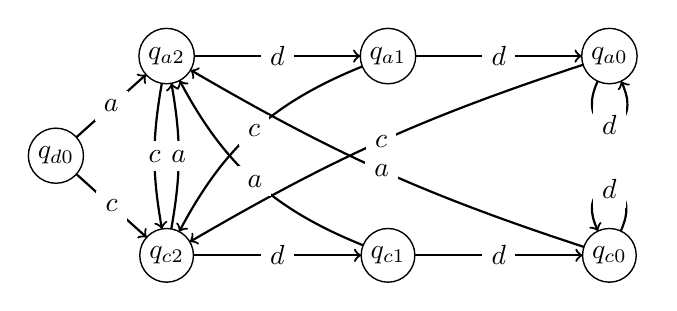
\begin{tikzpicture}[x=40,y=18]%
      \Vertex[L={$q_{d0}$}]{0}
      \NO[unit=2,empty=true](0){13}
      \EA[unit=1,L={$q_{a2}$}](13){12}
      \EA[unit=2,L={$q_{a1}$}](12){11}
      \EA[unit=2,L={$q_{a0}$}](11){10}
      \SO[unit=2,empty=true](0){33}
      \EA[unit=1,L={$q_{c2}$}](33){32}
      \EA[unit=2,L={$q_{c1}$}](32){31}
      \EA[unit=2,L={$q_{c0}$}](31){30}
      \tikzset{EdgeStyle/.style = {->}}
      \tikzset{LoopStyle/.style = {->}}
      \Edge[label=$a$](0)(12)
      \Edge[label=$d$](12)(11)
      \Edge[label=$d$](11)(10)
      \Edge[label=$c$](0)(32)
      \Edge[label=$d$](32)(31)
      \Edge[label=$d$](31)(30)
      \tikzset{EdgeStyle/.append style = {bend right=6}}
      \Edge[label=$c$](10)(32)
      \tikzset{EdgeStyle/.append style = {bend right=-6}}
      \Edge[label=$a$](30)(12)
      \tikzset{EdgeStyle/.append style = {bend right=20}}
      \Edge[label=$c$](11)(32)
      \tikzset{EdgeStyle/.append style = {bend right=-20}}
      \Edge[label=$a$](31)(12)
      \tikzset{EdgeStyle/.append style = {bend right=10}}
      \Edge[label=$c$](12)(32)
      \Edge[label=$a$](32)(12)
      \draw[thick,->] (10) to [out=-115,in=-65,looseness=7] node [midway, fill=white] {$d$} (10);
      \draw[thick,->] (30) to [out=65,in=115,looseness=7] node [midway, fill=white] {$d$} (30);
    \end{tikzpicture}
     \caption{Transitions and switchings between the \nodes{} for \exemref{cruise2}.
     \Nnodes{} $q_{b2}$, $q_{b1}$ and $q_{b0}$ are not shown for clarity.
     }
     \label{fig:cruise2}
  \end{figure}
\end{myexem}


\subsubsection{Discrete-Time Affine Hybrid Algebraic System}
\label{sec:dtahas}


\begin{mydef}[Invariant sets for a \dtahas{}]
  \label{def:is}
  Consider a \dtahas{} $\sys$ as in \defref{dtahas}.
  We say that sets $\Csetvar = (\Csetvar_q)_{q \in \Nodes}$ are \emph{invariant} for $\sys$ if
  $\Csetvar_q \subseteq \Ps_q$ for each $q \in \Nodes$ and
  for all $q \trs q'$,
  \begin{equation}
    \label{eq:isdtahas}
    A_\sigma \Csetvar_{q} + c_\sigma \subseteq E_\sigma \Csetvar_{q'}.
  \end{equation}
\end{mydef}

In view of \defref{is}, a trajectory of a \dtahas{} should be interpreted as follows.
Given initial conditions $x_0, q_0$, for each $k \ge 0$, a transition $q_k \trs[\sigma_{k}] q_{k+1}$
is first selected autonomously and then the state $x_k$ such that $E_{\sigma_{k}} x_{k+1} = A_{\sigma_{k}} x_k + c_{\sigma_{k}}$ can be controlled, knowing the selected transition.


\begin{myrem}
  \label{rem:descriptor}
  \defref{is} can be interpreted as stating that $\Csetvar$ is invariant if for each transition $q \trs q'$ and $x \in \Csetvar_q$,
  \begin{quote}
    there \emph{exists} $y \in \Csetvar_{q'}$ such that $A_\sigma x + c_\sigma = E_\sigma y$.
  \end{quote}
  A similar definition exists, see for instance \cite{liberzon2012switched},
  where this last part is replaced by
  \begin{quote}
    for \emph{each} $y$ such that $A_\sigma x + c_\sigma = E_\sigma y$, $y$ must belong to $\Csetvar_{q'}$.
  \end{quote}
  This is not equivalent to \defref{is} if $A_\sigma$ and $E_\sigma$ are not full rank
  as discussed in \remref{disturbvscontrol}.
  Moreover, computing ellipsoidal invariant sets according to this definition is much easier: it simply amounts to finding
  positive definite matrices $Q_q$ such that $A_\sigma^\Tr Q_q A_\sigma \preceq E_\sigma^\Tr Q_{q'} E_\sigma$; see \cite{owens1985consistency}.

  With this alternative definition of invariant sets, the invariance of sets of \dtahas{} would be equivalent to
  the robust invariance of sets for a system with disturbance.
  This differs from \propref{proju} for which the equivalence is with controlled invariance for a control system.
  This shows that, similarly to \cite{henrion2014convex, korda2014convex, korda2013inner},
  the LMI found in \cite{owens1985consistency} is related to robust invariance \eqref{eq:forall}
  and not control invariance~\eqref{eq:disc_existential}.
\end{myrem}

We now show that the computation of controlled invariant sets of a \dtahcs{} can be reduced to
the computation of invariant sets of a \dtahas{}.

\begin{myprop}
  \label{prop:proju}
  The sets $\Csetvar = (\Csetvar_q)_{q \in \Nodes}$ are \emph{controlled invariant} for the \dtahcs{}
  $\sys = (T, (A_\sigma, B_\sigma, c_\sigma)_{\sigma \in \Sigma}, (\Ps_q, \R^{\nqu})_{q \in \Nodes})$ if and only if
  they are invariant sets for the \dtahas{}
  $\sys' = (T, (E_\sigma A_\sigma, E_\sigma, E_\sigma c_\sigma)_{\sigma \in \Sigma}, (\Ps_q)_{q \in \Nodes})$
  where $E_\sigma = \pi_{\Image(B_\sigma)^{\perp}}$.

  \begin{proof}
    By \propref{projB}, as the input is unconstrained,
    for each $q \trs q'$ and $x \in \Ps_q$,
    there exists $u \in \R^{n_{q,u}}$ such that $A_\sigma x + B_\sigma u + c_\sigma \in \Csetvar_{q'}$ if and only if
    $E_\sigma A_\sigma x + E_\sigma c_\sigma \in E_\sigma \Csetvar_{q'}$.
  \end{proof}
\end{myprop}

In the following example, we apply \propref{proju} to \exemref{simplecontrol1}.

\begin{myexem}
  \label{exem:simplecontrol2}
  Consider the planar system introduced in \exemref{simplecontrol1}. In this system,
  $\Image(B)$ is the $u$-axis hence $\Image(B)^{\perp}$ is the $x$-axis.
  Hence we have
  \(
    A =
    \begin{bmatrix}
      1 & 1/2
    \end{bmatrix}
  \)
  and
  \(
    E =
    \begin{bmatrix}
      1 & 0
    \end{bmatrix}
  \).
\end{myexem}









\implementations{\jlpkg{SwitchOnSafety}.}





\part{Contributions}

\chapter{Set programming}
\label{chap:setprog}

In this chapter, we extend \chapref{opti} to optimization programs for which
decision variables are sets.
It is important to distinguish conic programs~\eqref{eq:conic_standard_form}, for which the decision variables are \emph{vectors} that belongs to \emph{given cones},
from set programs where the decision variables are \emph{sets}
that belongs to \emph{given families} of sets, called \emph{templates}.

This distinction is similar to the extension from first-order logic to second-order logic.
In first-order logic, propositions quantify only over variables that represent
elements of given sets while in second-order logic, propositions can quantify
over variables that can represent sets that are elements of given families of sets.
When considering sets inside propositions, Russell exhibited the famous Russell's
paradox: ``Let $\mathcal{S} = \setbuild{x}{x \notin x}$, then $\mathcal{S} \in \mathcal{S} \Leftrightarrow \mathcal{S} \notin \mathcal{S}$''.
This paradox is resolved in second-order logic by using a hierarchy of sets that can only contain sets of the lower order.
For instance, in second-order logic, the variables are sets that cannot contain sets themselves.
The same applies for set programming, the decision variables represent subsets of $\R^n$
or even convex subsets of $\R^n$ hence we shall not encounter Russell's paradox.

A key difference with the set programs we study in this section with the optimization of \emph{submodular functions} is that
the latter focuses on discrete sets while we focus on subsets of $\R^n$.
Given a finite set $\Omega$ and a set function $h: 2^{\Omega} \to \R$,
the function $f$ is \emph{submodular} if the condition\footnote{It is defined again later in~\eqref{eq:submodular1} but we include it here as well for convenience.}
holds for all subsets $\Jis, \Kis \subseteq \Omega$:
\begin{equation}
  \label{eq:submodular0}
  h(\Jis) + h(\Kis) \geq h(\Jis \cup \Kis) + h(\Jis \cap \Kis).
\end{equation}
The concept of \emph{submodular continuous functions} was introduced recently
but the functions are defined for continuous vectors, not subsets of a continuous domain.
Given a submodular function $h: 2^{[n]} \to \R$, we can define the function
$f: \{0, 1\}^{|\Omega|} \to \R$ with $f(x) = h(\setbuild{\omega \in [n]}{x_\omega = 1})$.
The submodularity condition~\eqref{eq:submodular0} is then rewritten as (see e.g. \cite[(1)]{bach2019submodular})
\[ f(x) + f(y) \ge f(\min(x, y)) + f(\max(x, y)) \]
where $\min$ and $\max$ are applied component-wise.
This condition is used to define submodular continuous functions
$f: [0, 1]^{|\Omega|} \to \R$.
If $f$ is twice differentiable, it is equivalent to
all off-diagonal entries of the hessian being nonpositives, see e.g. \cite[(2)]{bian2016guaranteed}.

A generic set program is defined as follows:
\begin{equation}
  \label{eq:setprog}
  \begin{array}{rl}
    \min\limits_{\mathcal{S}_1 \subseteq \R^{n_1}, \ldots, \mathcal{S}_N \subseteq \R^{n_N}} & f(\mathcal{S}_1, \ldots, \mathcal{S}_N)\\
    \text{subject to:} & g_i(\mathcal{S}_1, \ldots, \mathcal{S}_N) \subseteq h_i(\mathcal{S}_1, \ldots, \mathcal{S}_N), \quad i=1,2,\ldots,M.
  \end{array}
\end{equation}
where $\mathcal{S}_i \subseteq \R^{n_i}$ is a set decision variable, %
$f(\mathcal{S}_1, \ldots, \mathcal{S}_N)$ is the objective function
and the inclusion constraints are given by $g_i(\mathcal{S}_1, \ldots, \mathcal{S}_N) \subseteq h_i(\mathcal{S}_1, \ldots, \mathcal{S}_N)$ for $i = 1, \ldots, M$.
Note that this form also encapsulates membership constraints $x \in \mathcal{S}$
as it can be encoded as an inclusion constraint $\{x\} \subseteq \mathcal{S}$.

In this chapter, we give the following approach to set programs that is illustrated in \figref{setprog}:
\begin{enumerate}
  \item First, given the properties of gauge and support functions and the program constraints,
    we determine whether the set variables should be represented with the gauge or support function.
  \item Second, we consider the different templates and analyze the program
    obtained by formulating the program in terms of its gauge or support function,
    depending on what was determined in the previous section.
\end{enumerate}
The advantage of this approach is that the first step is independent of the
actual template and hence it gives a generic geometric approach to the computation
of sets that are solutions to the set program instead of the algebraic template-dependent approaches presented in \chapref{sys}.

For ellipsoids, piecewise semi-ellipsoids (resp. polysets and piecewise polysets),
specific classes of set programs can be reformulated as a semidefinite program (resp. Sum-of-Squares program).
The reformulation is done in the second step and, interestingly,
the interdependence of the different constraints and the objective only appears in
the choice of the representation, which is already carried out in
a template-independent fashion in the first step.
Therefore, the second-step can be done independently for the objective function
and for each constraint.
For this reason, we consider in each section,
the constraints and the objective functions in isolation.
Moreover, similarly to the bridges defined in \secref{bridges},
since each constraint can be reformulated independently,
implementing only a few constraint reformulation enables
the reformulation of programs made of any of their combinations,
as long as there is a valid choice of representation.

\begin{figure}
  \centering
  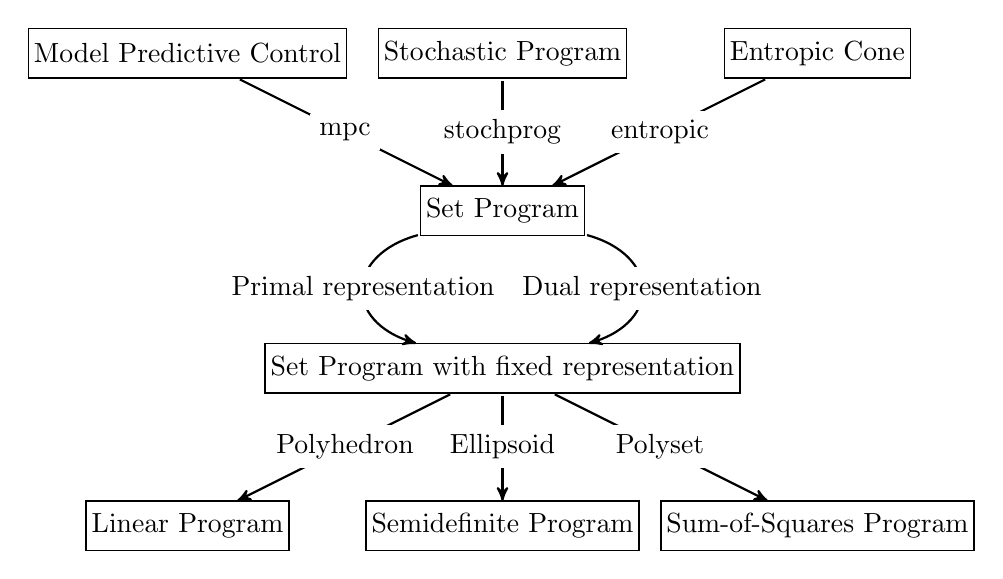
\begin{tikzpicture}[xscale=2]
    \SetVertexNormal[Shape=rectangle]
    \SetUpEdge[style={post,thick}]
    \Vertex[L={Set Program}]{1}
    \NOWE[L={Model Predictive Control},unit=2](1){6}
    \Edge[label={\secref{mpc}}](6)(1)
    \NO[L={Stochastic Program},unit=2](1){7}
    \Edge[label={\secref{stochprog}}](7)(1)
    \NOEA[L={Entropic Cone},unit=2](1){8}
    \Edge[label={\chapref{entropic}}](8)(1)
    \SO[L={Set Program with fixed representation},unit=2](1){2}
    \SO[L={Semidefinite Program},unit=2](2){3}
    \Edge[label={Ellipsoid}](2)(3)
    \SOEA[L={Sum-of-Squares Program},unit=2](2){4}
    \Edge[label={Polyset}](2)(4)
    \SOWE[L={Linear Program},unit=2](2){5}
    \Edge[label={Polyhedron}](2)(5)
    \SetUpEdge[style={post,thick,bend right=60}]
    \Edge[label={Primal representation}](1)(2)
    \SetUpEdge[style={post,thick,bend right=-60}]
    \Edge[label={Dual representation}](1)(2)
  \end{tikzpicture}

  \caption{
    Illustration of the advantages of the set programming interface.
    It first allows different applications such as Model Predictive Control,
    Stochastic Programming and the Entropic Cone to formulate the set
    program that should be solved in a template independent manner.
    Second, the choice between primal representation (e.g. gauge function)
    or dual representation (e.g. support function) is done in a template independent manner.
    Lastly, once the representation is determined for each set, each inclusion constraint
    can be reformulated independently of the rest of the set program.
  }
  \label{fig:setprog}
\end{figure}

\begin{myexem}
  \label{exem:simplesetprog}
  Consider the following generic set program modeling the controlled
  invariance of the control system considered in \exemref{simplecontrol1} and \exemref{simplecontrol2}:
  \begin{align}
    \notag
    \maxi_{\mathcal{S}} \vol(\mathcal{S})\\
    \label{eq:inclsquareexem}
    \mathcal{S} & \subseteq [-1, 1]^2\\
    \label{eq:alginclexem}
    C\mathcal{S} & \subseteq E\mathcal{S}.
  \end{align}
  where
  \(
    C =
    \begin{bmatrix}
      1 & 1/2
    \end{bmatrix}
  \)
  and
  \(
    E =
    \begin{bmatrix}
      1 & 0
    \end{bmatrix}
  \).

  As discussed in \secref{preimage}, due to \eqref{eq:alginclexem},
  it is more appropriate to choose the dual representation (i.e. support function)
  for this program, independently of the template.

  For the ellipsoids template, the dual representation is given by
  $\supfun{y}{\mathcal{S}} = \sqrt{x^\Tr Q x}$ as shown in \propref{supfunell}.
  By \eqref{eq:revincl},
  the inclusing \eqref{eq:inclsquareexem} is equivalent to
  $(1, 1), (-1, 1), (1, -1), (-1, -1) \in \polar{\mathcal{S}} = \mathcal{E}_{Q}$
  which can be encoded as a linear constraint with \eqref{eq:vinell1}.
  As we will see in \secref{preimage},
  \eqref{eq:alginclexem} can be encoded as the LMI~\eqref{eq:ellalgincl}.
  In this case, as $C, E$ have only one row, this LMI has dimension $1 \times 1$
  so it is the linear inequality $Q_{1,2} + Q_{2,2}/4 \le 0$.
  The optimal ellipsoid $\Ell{Q^{-1}}$ and its polar $\Ell{Q}$ are given
  respectively in \figref{SimpleControlledInvariantEllipsoid}
  and \figref{SimpleControlledInvariantPolarEllipsoid}.

  For the polyset template of degree $2d$, the dual representation is given by
  $\supfun{y}{\mathcal{S}} = \sqrt[2d]{p(x)}$ where $p(x)$ is a homogeneous
  polynomial of degree $2d$.
  We use the volume heuristic
  consisting in maximizing the integral of $p(x)$ over the square $[-1, 1]^2$.
  This is the method of \cite{dabbene2017simple} discussed in \secref{polysetvol}.
  The optimal solution is given in \figref{SimpleControlledInvariantPoly}.

  For the piecewise semi-ellipsoidal template,
  the volume is not directly maximized.
  Instead, for each cone of the partition,
  we compute the sum $s$ of the normalized rays and consider the polytope obtained by intersecting the cone with the halfspace
  $s^\top x \le \|s\|_2^2$.
  We integrate the quadratic form corresponding to this cone,
  i.e. $h^2(\mathcal{S}, x)$ over the polytope.
  The sum of the integrals over each polytope is the objective function we use.
  This can be seen as the generalization of the sum of the squares of the length of the semi-axes
  of the polar of the ellipsoid.

  The conic partition is obtained by considering the conic hull of each facets of a given polytope.
  We first consider the conic partition corresponding to the polar of the square $[-1, 1]^2$.
  This gives the four quadrants as cones of the conic partition.
  The maximal piecewise semi-ellipsoidal control invariant set with this partition has the following support function:
  $$
  \supfun{x}{\mathcal{S}}^2 = \begin{cases}
  (x_1 - x_2)^2 & \text{ if }x_1x_2 \le 0,\\
  x_1^2 - x_1x_2/2 + x_2^2 & \text{ if }x_1x_2 \ge 0.
  \end{cases}
  $$
  For the cones $x_1x_2 \le 0$, the semi-ellipsoid matches the square and the maximal control invariant set.
  For the cones $x_1x_2 \ge 0$, the semi-ellipsoid matches the optimal solution for the ellipsoid of maximal volume.
  This illustrates one key feature of piecewise semi-ellipsoidal sets, they can combine advantages of both polyhedra and ellipsoids.
  It can be polyhedral on the directions where the maximal control invariant set is polyhedral and be ellipsoidal on the directions where the maximal control invariant set is smooth or requires many halfspaces in its representation.
  We can use the polar of the polytope resulting from the first fixed point iteration to generate a refined conic partition.
  With this partition, the optimal solution for piecewise semi-ellipsoids matches the optimal solution of the generic set program. The support function is given by:
  $$
  \supfun{x}{\mathcal{S}}^2 = \begin{cases}
  (x_1 - x_2)^2 & \text{ if }x_1x_2 \le 0,\\
  x_1^2 & \text{ if }x_2(x_1-2x_2) \ge 0,\\
  (x_1/2 + x_2)^2 & \text{ if }x_1(2x_2-x_1) \ge 0.\\
  \end{cases}.
  $$

  For the polyhedral template, there are several choices of parametrization of the
  representation.
  We consider two cases here and highlight that in both cases,
  it is more appropriate to use the dual representation,
  that is, the support function of $\mathcal{S}$ which is given by the
  V-representation of $\mathcal{S}$ or equivalently the H-representation of
  $\polar{\mathcal{S}}$.
  This supports the template-independence of this choice of representation.

  The V-representation of both $C\mathcal{S}$ and $E\mathcal{S}$ depends linearly on the V-representation of $\mathcal{S}$ as shown in \propref{hApolyhedron}.
  The inclusing is ensured by constraining each element of the V-representation
  of $C\mathcal{S}$ to belong to $E\mathcal{S}$ using \propref{vinvrep} and \propref{rinvrep}.
  If the coordinates of each element of the V-representation of $\mathcal{S}$ is fixed,
  this give a linear program to verify that $\mathcal{S}$ is a feasible solution.
  Otherwise, if the coordinates of the elements are to be determined
  it gives a bilinear program.
  This condition is given in \cite[Theorem~4.44]{blanchini2015set}.
  Note that there is no corresponding result for the H-representation in \cite{blanchini2015set}.
  This is in accordance with the claim of \secref{preimage} that the dual representation
  should be used for such inclusion.

  Alternatively, given a fixed partition, the support function can be given by
  \[
    \supfun{y}{\mathcal{S}} =
    \la a_i, y \ra \text{ if } y \in \mathcal{P}_i.
  \]
  In this case, by \propref{hA}, we have
  \[
    \supfun{y}{C\mathcal{S}} =
    \la C a_i, y \ra \text{ if } y \in C^\Tr \mathcal{P}_i.
  \]
  Therefore, $C\mathcal{S} \subseteq E\mathcal{S}$ is equivalent to
  \[ \forall i, j, (E a_j - C a_i) \in C^\Tr \mathcal{P}_i \cap E^\Tr \mathcal{P}_j. \]
  If the partition is fixed, this is rewritten as linear constraints using \propref{hinhrep}.
  This representation of polyhedra is studied in \cite{rakovic2020robust}.
\end{myexem}

\begin{figure}[!ht]
  \centering
  \begin{subfigure}[b]{0.45\textwidth}
      \includegraphics[trim=3.7cm 0cm 3.9cm 0cm, clip, width=\textwidth]{SimpleControlledInvariantEllipsoid.png}
      \caption{Primal space}
      \label{fig:SimpleControlledInvariantEllipsoid}
  \end{subfigure}
  ~ %
  \begin{subfigure}[b]{0.45\textwidth}
      \includegraphics[trim=3.7cm 0cm 3.9cm 0cm, clip, width=\textwidth]{SimpleControlledInvariantPolarEllipsoid.png}
      \caption{Polar space}
      \label{fig:SimpleControlledInvariantPolarEllipsoid}
  \end{subfigure}
  \caption{Optimal solutions for the set program of \exemref{simplesetprog}.
  The green set is the square $[-1, 1]^2$,
  the yellow set is the optimal solution of the generic set program,
  the blue ellipsoid is the optimal solution of the set program for ellipsoids
  and the red ellipsoid is the optimal solution of the set program for ellipsoids with the objective replaced by the sum of squares of the length of the semi-axes of the polar.}
  \label{fig:SimpleControlledInvariantEll}
\end{figure}

\begin{figure}[!ht]
  \centering
  \begin{subfigure}[b]{0.45\textwidth}
      \includegraphics[trim=3.7cm 0cm 3.9cm 0cm, clip, width=\textwidth]{SimpleControlledInvariantPiecewiseSemiEllipsoid.png}
      \caption{Primal space}
      \label{fig:SimpleControlledInvariantPiecewiseSemiEllipsoid}
  \end{subfigure}
  ~ %
  \begin{subfigure}[b]{0.45\textwidth}
      \includegraphics[trim=3.7cm 0cm 3.9cm 0cm, clip, width=\textwidth]{SimpleControlledInvariantPolarPiecewiseSemiEllipsoid.png}
      \caption{Polar space}
      \label{fig:SimpleControlledInvariantPolarPiecewiseSemiEllipsoid}
  \end{subfigure}
  \caption{
    Optimal solutions for the set program of \exemref{simplesetprog}.
    The green set is the square $[-1, 1]^2$ and
    the blue and yellow sets are the optimal solutions of the set program for piecewise semi-ellipsoids
    with the objective replaced by the integral of $\supfun{y}{\mathcal{S}}^2$ over
  the polar of the square
    and with different conic partitions.
  }
  \label{fig:SimpleControlledInvariantPiecewiseSemiEll}
\end{figure}

\begin{figure}[!ht]
  \centering
  \begin{subfigure}[b]{0.45\textwidth}
      \includegraphics[trim=3.7cm 0cm 3.9cm 0cm, clip, width=\textwidth]{SimpleControlledInvariantPolySet.png}
      \caption{Primal space}
      \label{fig:SimpleControlledInvariantPolySet}
  \end{subfigure}
  ~ %
  \begin{subfigure}[b]{0.45\textwidth}
      \includegraphics[trim=3.7cm 0cm 3.9cm 0cm, clip, width=\textwidth]{SimpleControlledInvariantPolarPolySet.png}
      \caption{Polar space}
      \label{fig:SimpleControlledInvariantPolarPolySet}
  \end{subfigure}
  \caption{Optimal solutions for the set program of \exemref{simplesetprog}.
  The green set is the safe set $[-1, 1]^2$,
  the yellow set is the optimal solution of the generic set program,
  the optimal solution of the set program for polysets of
  degree 4, (resp. 8, 18 and 22) is represented in orange (resp. blue, green
  and red).
  Note that, as discussed in \cite[Remark~2]{dabbene2017simple}, their heuristic
  coincides with the sum of squares of semi-axes for quadratic forms.
  For this reason, the optimal controlled invariant sublevel set of quadratic
  forms is the red ellipsoid in \figref{SimpleControlledInvariantEll}.}
  \label{fig:SimpleControlledInvariantPoly}
\end{figure}

In \secref{representation}, we discuss the choice of representation depending on
the objective and constraints.
In \secref{objective}, we discuss different types of objective functions and different ways to handle each type depending on the template of the sets involved in the objective function.

In \secref{image} and \secref{preimage}, we investigate the following four types of functions $f_i$, $g_i$ in the inclusion constraints of the set program.
\begin{align*}
  (\mathcal{S}_1, \ldots, \mathcal{S}_N) & \mapsto \mathcal{S}_j, & & \text{ where }j \in [N]\\
  (\mathcal{S}_1, \ldots, \mathcal{S}_N) & \mapsto A\mathcal{S}_j, & & \text{ where }j \in [N], A \in \R^{m \times n_j}\\
  (\mathcal{S}_1, \ldots, \mathcal{S}_N) & \mapsto A^{-1}\mathcal{S}_j, & & \text{ where }j \in [N], A \in \R^{n_j \times m}\\
  (\mathcal{S}_1, \ldots, \mathcal{S}_N) & \mapsto \pi_{[n_k], m} A^{-1}\mathcal{S}_j, & & \text{ where }j, k \in [N], A \in \R^{n_j \times m}.
\end{align*}
In particular, in \secref{image} we focus on constraints of the form
\begin{align}
  \label{eq:imageincl}
  A\mathcal{S}_i & \subseteq \mathcal{S}_j,\\
  \label{eq:preimageincl}
  \mathcal{S}_i & \subseteq A^{-1}\mathcal{S}_j.
\end{align}
with $A \in \R^{n_j \times n_i}$.
In \secref{preimage}, we focus on constraints of the form
\begin{align}
  \label{eq:projectpreimageincl}
  \mathcal{S}_i & \subseteq \pi_{[n_i], n_i + m}
  \begin{bmatrix}
    A & B
  \end{bmatrix}^{-1} \mathcal{S}_j,\\
  \label{eq:algincl}
  C\mathcal{S}_i & \subseteq E\mathcal{S}_j.
\end{align}
with $A \in \R^{n_j \times n_i}, B \in \R^{n_j \times m}$, $C \in \R^{r \times n_i}$ and $E \in \R^{r \times n_j}$.

In \secref{special}, we study two variants of set programs consisting in finding the
minimal or maximal scaling of a hypersphere in a hypercube.
We show small changes in the set program can have dramatic effect on complexity.

When $g_i$ is a union or $h_i$ is an intersection, the constraint can be split into
several constraints.
When $g_i$ is an intersection of $h_i$ is a union,
one typically needs to employ \propref{lossysproc} for ellipsoids
or more generally \cororef{positiv} for polysets.
In \secref{john}, we study the problem of finding the minimal value of $\gamma$
and an ellipsoid $\mathcal{E}_P$ such that a given intersection of ellipsoids includes $\mathcal{E}_P$ and is included in $\gamma\mathcal{E}_P$.
Note that, by \lemref{convcap} and \propref{polarell}, this is equivalent to having the convex hull of their union include $\mathcal{E}_{P^{-1}}/\gamma$ and be included in $\mathcal{E}_{P^{-1}}$.

We assume in this chapter that the sets $\mathcal{S}_i$ contain the origin.
It might not always be the case, and a translation might not always make it possible.
For instance, we might have constraints $\mathcal{S}_1 \subseteq \Pset_1$ and
$\mathcal{S}_2 \subseteq \Pset_2$ where $\Pset_1, \Pset_2$ are two disjoint given polyhedra.
In this case, there is no tranlation of the state space that ensure that
both $\mathcal{S}_1$ and $\mathcal{S}_2$ contain the origin.
In \secref{homogenization}, we discuss how to lift the state space to handle this non-homogeneity.

\section{Representation}
\label{sec:representation}
As highlighted in the introduction, for each variable of the set program,
we should choose whether the variable is represented using its primal representation (i.e. gauge function) or dual representation (i.e. support function).
To determine the representation to use for each variable, we analyse the impact
of the choice for the objective and each constraint.

For the objective, if the integral heuristic discussed in \secref{volobj} is used
then either the primal or dual representation can be used as
the integral can be done either on the gauge or support function with either
maximization or minimization as the integral depends linearly on the parameters
of the representation.
However, for the $\log \det \cdot$ and $\sqrt[n]{\det \cdot}$ objective for
the ellipsoidal template, the representation is determined by the sense
of the objective as discussed in \secref{ellvol}.

For constraints,
as discussed in \secref{image},
constraints of the form
\eqref{eq:imageincl} and \eqref{eq:preimageincl} requires that the sets have
the same representation and,
as discussed in \secref{image},
constraints of the form
\eqref{eq:projectpreimageincl} and \eqref{eq:algincl} requires that the sets both
have the dual representation.

Some constraints may also have ``soft preferences'' instead of ``hard constraints''.
For instance, consider a constraint $\mathcal{S} \subseteq \mathcal{P}$
where $\mathcal{S}$ is an ellipsoid and $\mathcal{P}$ is a polyhedron.
If the primal representation is used for $\mathcal{S}$ and the polyhedron $\mathcal{P}$
is fixed,
the LMI \eqref{eq:ellinh3} should be used.
If the polyhedron has a parametrized H-representation then \eqref{eq:ellinh2}
should be used instead.
If the dual representation is used for $\mathcal{P}$ and the polyhedron $\mathcal{P}$
is fixed, then the linear constraint \eqref{eq:ellinh1}.
We see here that if the polyhedron $\mathcal{P}$ is fixed,
then the dual representation is preferred as it creates a linear constraints
while the primal representation creates an LMI.
A similar discussion applies, for a constraint $\mathcal{P} \subseteq \mathcal{S}$
with \propref{vinell}.
If there is no hard constraint on the representation of $\mathcal{S}$,
these soft preferences can be used to generate a semidefinite program that
is less computationally expensive to solve.

\section{Objective}
\label{sec:objective}
There can be multiple different types of objective functions to a set program.
\begin{itemize}
  \item
    First, a \emph{feasibility} set program has no objective function, this is the case in \chapref{stab}.
  \item
    Second, we might want to maximize or minimize a linear combination of the volumes of the set variables.
    This is the objective chosen in \chapref{mci}.
  \item
    Third, we might want to maximize a set variable $\mathcal{S}$ in a specific direction (see \cite{ahmadi2018robust} for a detailed analysis for a special case of set program with directional objective).
    For instance, we might to maximize $\gamma$ such that $\gamma x \subseteq \mathcal{S}$ for a given vector $x$, or minimize $\gamma$ such that $\mathcal{S} \gamma \subseteq \halfspace{a}{\alpha}$.
    This is the case of the \emph{Ingleton score} studied in \chapref{entropic}, see \eqref{eq:ingleton}.
\end{itemize}

The second type of objective is detailed in \secref{volobj} and the third one is discussed in \secref{dirobj}.

\subsection{Volume objective}
\label{sec:volobj}

In view of \propref{gaugelikeincl} (resp. \propref{supportincl}), minimizing (resp. maximizing) the integral of the gauge-like (resp. support) function
over a given set is a sensible heuristic for maximizing the volume.
In fact, the volume can be computed directly from the gauge function
with the following proposition.
\begin{myprop}[{\cite{campi2006volume}}]
  The $n$-dimensional volume of a convex body $\Cset \subseteq \R^n$ is given by
  \begin{equation}
    \label{eq:gaugevol}
    \frac{1}{n} \int_{\Sn} \gauge^{-n}(\Cset, x) \dif x.
  \end{equation}
\end{myprop}
However, the expression~\eqref{eq:gaugevol} may not be easy to optimize on as
it may not be a convex function in terms of the parametrization of a set for a given template.

\subsubsection{Ellipsoid volume}
\label{sec:ellvol}
As shown in \propref{detell}, in order to maximize (resp. minimize) the volume of an ellipsoid
$\mathcal{E}_P$, the determinant $\det P$ should be minimized (resp. maximized).
\remref{sdpvol} discusses how to optimize $\det P$ depending on the SDP solver capabilities.
If the $\ln\det P$ is not natively supported by the solver and need to be reformulated,
a $(2n) \times (2n)$ LMI constraint is added.
In view of \remref{psdsize}, this might substantially increase the solve time of the semidefinite program.
Moreover, this objective is reformulated into exponential cone constraints.
If these constraints are not supported, the objective $\sqrt[n]{\det P}$
can be used instead which can be reformulated into a $(2n) \times (2n)$ LMI constraint
and rotated second-order cone constraints.
As the $\ln\det P$ and $\sqrt[n]{\det P}$ functions are concave in $P$,
they should be maximized in order for the program to be convex.
Therefore, if the volume of an ellipsoid is maximized (resp. minimized),
it should be represented as $\mathcal{E}_{P^{-1}}$ (i.e. the dual representation) (resp. $\mathcal{E}_{P^{-1}}$ (i.e. the primal representation)).

Alternatively, the integral of the gauge-like function of degree 2 over a given set can be minimized.
By linearity, the integral can be expressed as a linear combination of the entries of $Q$, multiplied by the integral of the corresponding monomial.
It turns out that if this set is the hypercube symmetric around the origin,
then this integral is exactly twice the trace of $P$. %
In view of \propref{trell}, this is twice the sum of the squares of the length of the semi-axes of $\mathcal{E}_P$.

These two ways to maximize the ``size'' of the set are discussed in \cite{durieu1996trace}.
Even if the trace of $P$ does not correspond to the volume,
this objective may render the set ``larger'' than using the volume for
some instances of set programs.
We compare these as well in \exemref{simplesetprog}, \figref{SimpleControlledInvariantEll}.

\subsubsection{Polyset volume}
\label{sec:polysetvol}

We discuss in this section three methods for maximizing the volume of a polyset $\polyset[p]$.
A first method is to minimize the integral of the gauge-like function of degree $2d$ over a given set.
By linearity, the integral can be expressed as a linear combination of the coefficient of the polynomials, multiplied by the integral of the corresponding monomial.
The linearity of the expression is appealing as it directly fits in the linear objective of \eqref{eq:sdp_standard}.
This method is discussed further in \cite{dabbene2017simple},

A second (resp. third) method is to minimize the volume of $\mathcal{E}_Q$ where
$Q$ is the positive semidefinite matrix certifying that $p(x)$ is SOS-convex (resp. SOS).
Note that both methods correspond to the minimization of $\det P$ for an ellipsoid $\mathcal{E}_P$ that was discussed in \secref{ellvol}.
The second method is developed in \cite{magnani2005tractable} and we detail the third
method in the remaining of this section.

As discussed in \secref{sosprog}, if we choose some polynomial basis $b$,
there exists some positive semidefinite matrix $Q \in \Psd$ such that
$p(x) = \elli{Q}{b}$ so $p(x)$ can be seen as an ellipsoid in a lifted space~\cite{philippe2015stability}.

More precisely, consider the basis $b = \ld{x}$ and the following operator on sets $\Sset^{[d]} = \{\, x^{[d]} \mid x \in \Sset \,\}$.
Given an SOS polynomial $p(x) = \la \ld{x}, Q \ld{x} \ra$ where $Q \in \Psd$,
we have the following identity
\[ \ld{(\polyset[p])} = \mathcal{E}_Q \cap (\R^n)^{[d]}. \]
That is, $\ld{(\polyset[p])}$ is the intersection of a semi-ellipsoid and the \emph{Veronese variety} $\ld{(\R^n)}$.

\begin{myexem}
  Consider the polynomial $p(x) = (x_1^2 + x_2^2)^2 = x_1^4 + 2x_1^2x_2^2 + x_2^4$.
  We consider the scaled monomial basis introduced in \secref{sosprog}.
  The Veronese variety is given by
  \[ (\R^2)^{[2]} = \setbuild{(x_1^2,x_2^2,x_1x_2)}{x \in \R^2} = \setbuild{y}{y_3^2 = y_1y_2}. \]
  The set $\ld{(\polyset[p])}$ is the intersection of the ellipsoid $\setbuild{y}{y_1^2 + y_2^2 + 2y_3^2 \leq 1}$ with $(\R^2)^{[2]}$.
  This is illustrated by \figref{vero}.
\end{myexem}

\begin{figure}[!ht]
  \centering
  \begin{subfigure}{0.49\textwidth}
    \includegraphics[width=\textwidth]{left.png}
  \end{subfigure}
  \begin{subfigure}{0.49\textwidth}
    \includegraphics[width=\textwidth]{right.png}
  \end{subfigure}
  \caption{Illustration for the Veronese variety.}
  \label{fig:vero}
\end{figure}

In view of the preceding discussion, instead of minimizing the volume of $\ld{(\polyset[p])}$,
it does not seem unreasonable to minimize the volume of the ellipsoid $\mathcal{E}_Q$ which is easily computable thanks to \propref{detell}.
Note however that there is a whole affine space of matrices $Q$ such that $p(x) = \la x^{[d]},  Q x^{[d]} \ra$ so $Q$ can be chosen in the intersection of this affine space with the cone $\Psd$ of semidefinite matrices.

\subsection{Directional objective}
\label{sec:dirobj}

Suppose the objective is to maximize $\gamma$ such as $\gamma x \in \mathcal{S}$ for a fixed vector $x$.
For polysets, ellipsoids and their piecewise versions as template for $\mathcal{S}$,
since the approach is to
reformulate the set program as an SOS program, we simply set the linear objective function to $\gamma$ and add the constraint $\gamma x \in \mathcal{S}$.

If the template for $\mathcal{S}$ is polyhedral,
then the method used to compute $\mathcal{S}$ might be completely different from
the classical iterative approaches.
One drawback of these iterative approaches is that it refines the polyhedral
approximation of the optimal value of $\mathcal{S}$ in the generic program
in every direction.
However, an accurate polyhedral approximation of this set might need a polyhedral representation of prohibitive size.
This curse of dimensionality can be circumvented in the case of a directional objective.
\algoref{cutgen}, introduced in \secref{ddp},
can be used to generate cuts to refine a polyhedral approximation in some desired directions only.
Consider for instance the following set program with inclusion constraints of the form~\eqref{eq:algincl} and a directional objective.
\begin{equation}
  \label{eq:dirproj}
  \begin{array}{rl}
    \min\limits_{\mathcal{S}_1 \subseteq \Pset_1, \ldots, \mathcal{S}_N \subseteq \Pset_N} & \gamma\\
    \text{subject to:} & \gamma x \in \mathcal{S}_1\\
    & A_k \mathcal{S}_{i_k} \subseteq E_k \mathcal{S}_{j_k}, k = 1 \ldots, M\\
  \end{array}
\end{equation}

We can start with the solutions $\mathcal{S}_i \gets \Pset_i$ and
we can iteratively find the maximum $\gamma$ such that $\gamma x \in \mathcal{S}_1$,
then check whether this satisfy all constraints and if it does not, generate
an infeasibility cut as in \algoref{cutgen}.
This procedure is detailed in \algoref{dirobj}.
It searches over the tree of depth $D$ of all the paths of length $D$ starting at node 1 in the graph underlying the set program where the constraint $k$ is a directed edge from node $i_k$ to $j_k$.
In the context of \emph{Stochastic Programming} introduced in \secref{stochprog},
this tree is made of the \emph{forward pass},
$d$ represents the \emph{time} or \emph{stage} (see \remref{stages}),
$i$ represents the current node of the markov chain,
the integers $k$ such that $i_k = i$ are the transitions index of constraints of \eqref{eq:dirproj} corresponding to transitions with source $i$
and $j_k$ is the target of the transition.

In Stochastic Programming, instead of generating the cuts ``on the fly'' during the forward pass as done in \algoref{dirobj}, they are
generated in a \emph{backward pass} that start from the leaves of the tree, and generate for each leaf the cut for the node before the leaf in the path ending at this leaf.
Then, it generates the cut in the nodes preceding these nodes where a cut was added.
The advantage of this approach is that the newly generated cut is used when
generating the cuts of the previous nodes in the tree.
Indeed, if the cuts where generated forward instead of backward, we would need
$D$ pass for a cut in the end of a path of length $D$ to impact a node in the
start of the path!
Moreover, once an infeasibility is found somewhere in the tree,
a packward pass can generate infeasibility cuts up to the node 1 at the start of the path
and then the rest of the search tree can be aborted.
Indeed, there is no need for generating more than one infeasibility cut for ensuring
that $\opt{\gamma} x$ will not be found again.
These two improvements: backward pass and early abortion should be applied to
\algoref{dirobj} in order to improve its practical efficiency.

Another important practical aspect is the order in which the elements are
chosen in the set $I$ of \algoref{dirobj}.
Indeed, with the early abortion approach presented in the previous paragraph,
it is derisable to choose an element in $I$ for that will generate an infeasibility
cut as early as possible.
Depending on the nature of the instance of the set program \eqref{eq:dirproj},
different ordering may be more appropriate.
For some instances, it may be relevant to record the paths in the tree that generate infeasibility cuts more frequently and visit them in priority.
It is important to average the number of cuts generated over the number of times they are visited.
Indeed, the paths that are visited in priority might generate more cuts hence be even more priorized, this could lead to some paths being neglected.

\begin{algorithm}[!ht]
  \caption{Solving a set program with polyhedral set variables and directional objective.}
  \label{algo:dirobj}
  \begin{algorithmic}
    \STATE \textbf{Input} A program~\eqref{eq:dirproj} and a maximal depth $D$.
    \STATE Set $\mathcal{S}_i \gets \Pset_i$.
    \REPEAT
      \STATE Set $\opt{\gamma} \in \argmax \setbuild{\gamma}{\gamma x \in \mathcal{S}_1}$.
      \STATE Set $x_1 \gets \opt{\gamma} x$.
      \STATE Set $I = \{(1, \opt{\gamma} x, 0)\}$.
      \WHILE{$I \neq \emptyset$}
        \STATE Choose $(i, y, d) \in I$.
        \IF{$d < D$}
          \FORALL{$k = 1 \ldots, M$}
            \IF{$i_k = i$}
              \STATE Search for $z \in \mathcal{S}_{j_k}$ such that $A_k y = E_k z$.
              \IF{This is feasible, a feasible solution $z$ is found}
                \STATE Set $I \gets I \cup \{(j_k, z, d + 1)\}$.
              \ELSE
                \STATE Generate an infeasibility cut $\halfspace{a}{\alpha}$ from the infeasibility ray as in \algoref{cutgen}. %
                \STATE Set $\mathcal{S}_i \gets \mathcal{S}_i \cap \halfspace{a}{\alpha}$.
              \ENDIF
            \ENDIF
          \ENDFOR
        \ENDIF
        \STATE Set $I \gets I \setminus \{(i, y, d)\}$.
      \ENDWHILE
    \UNTIL{No infeasibility cut is generated in the loop}
  \end{algorithmic}
\end{algorithm}

\section{Inclusion with one linear image or a preimage}
\label{sec:image}

We can see with \propref{image} that the constraint~\eqref{eq:imageincl} and the constraint~\eqref{eq:preimageincl} are equivalent.

\begin{myprop}
  \label{prop:image}
  Consider a matrix $A \in \R^{n_1 \times n_2}$, a set $\mathcal{S} \subseteq \R^{n_2}$ and a set $\mathcal{T} \subseteq \R^{n_1}$.
  The inclusion $A\mathcal{S} \subseteq \mathcal{T}$ holds if and only if
  the inclusion $\mathcal{S} \subseteq A^{-1}\mathcal{T}$ holds.
  \begin{proof}
    The inclusion $A\mathcal{S} \subseteq \mathcal{T}$
    is equivalent to $x \in \mathcal{S} \Rightarrow Ax \in \mathcal{T}$.
    Since $Ax \in \mathcal{T}$ is equivalent to $x \in A^{-1}\mathcal{T}$,
    we have the desired result.
  \end{proof}.
\end{myprop}

\begin{myrem}
  \label{rem:image}
  Note that $\mathcal{S} \subseteq A\mathcal{T}$
  does not imply $A^{-1}\mathcal{S} \subseteq \mathcal{T}$.
  For instance, if
  $A = \begin{bmatrix} 1 & 0
  \end{bmatrix}$,
  $\mathcal{S} = [-1, 1]$ and $\mathcal{T} = [-1, 1]^2$ then
  $\mathcal{S} = [-1, 1] = A\mathcal{T}$ but
  $A^{-1}\mathcal{S} = [-1, 1] \times \R \not\subseteq \mathcal{T}$.
\end{myrem}

We can formulate inequalities in terms of either the support (resp. gauge) function of $\mathcal{S}_i$ and $\mathcal{S}_j$
with \eqref{eq:suppASS} (resp. \eqref{eq:gaugeSAS}) or
we can write them in terms of the gauge (resp. support) function of the polar of $\mathcal{S}_i$ and $\mathcal{S}_j$
with \eqref{eq:gaugeASS} (resp. \eqref{eq:suppSAS}).
\begin{mytheo}
  \label{theo:gaugesupp_image}
  Consider closed convex sets $\mathcal{S}_i, \mathcal{S}_j$ containing the origin.
  The equivalent constraints \eqref{eq:imageincl} and \eqref{eq:preimageincl}
  are equivalent to each of the following equivalent inequalities:
  \begin{align}
    \label{eq:suppASS}
    \forall y &\in \mathbb{R}^{n_j}, & \supfun{A^\Tr y}{\mathcal{S}_i} & \le \supfun{y}{\mathcal{S}_j}.\\
    \label{eq:gaugeSAS}
    \forall x &\in \mathbb{R}^{n_i}, & \gauge(\mathcal{S}_i, x) & \ge \gauge(\mathcal{S}_j, A x).\\
    \label{eq:gaugeASS}
    \forall y &\in \mathbb{R}^{n_j}, & \gauge(\polar{\mathcal{S}_i}, A^\Tr y) & \le \gauge(\polar{\mathcal{S}_j}, y).\\
    \label{eq:suppSAS}
    \forall x &\in \mathbb{R}^{n_i}, & \supfun{x}{\polar{\mathcal{S}_i}} & \ge \supfun{A x}{\polar{\mathcal{S}_j}}.
  \end{align}
  \begin{proof}
    Using \eqref{eq:imageincl} and \propref{hA}, we obtain \eqref{eq:suppASS}.
    Using \eqref{eq:preimageincl} and \propref{gA}, we obtain \eqref{eq:gaugeSAS}.
    Using \eqref{eq:suppASS} and \propref{gaugesupp}, we obtain \eqref{eq:gaugeASS}.
    Using \eqref{eq:gaugeSAS} and \propref{gaugesupp}, we obtain \eqref{eq:suppSAS}.
  \end{proof}
\end{mytheo}

\subsection{Ellipsoid template}
For ellipsoidal sets $\mathcal{S}_i = \mathcal{E}_{Q_i}$, as defined in \eqref{eq:ell}, the inequality \eqref{eq:gaugeSAS}
can be rewritten in terms of the matrices $Q_i$ as:
\begin{equation}
  \label{eq:ellprimageincl}
  Q_i \succeq A^\Tr Q_j A.
\end{equation}
This LMI could alternatively be obtained in a more template-specific way from the inclusion~\eqref{eq:preimageincl}
with \propref{ellpreimage} and \propref{ellincl}.

On the other hand, the inequality \eqref{eq:suppASS}
can be rewritten in terms of the matrices $Q_i^{-1}$ as:
\begin{equation*}
  A Q_i^{-1} A^{\Tr} \preceq Q_j^{-1}.
\end{equation*}
This LMI could alternatively be obtained in a more template-specific way from the inclusion~\eqref{eq:imageincl}
with equation~\eqref{eq:supfunellimage} of \propref{ellimage} and \propref{supportincl}.

\subsection{Piecewise semi-ellipsoid template}
For a piecewise semi-ellipsoidal set, \eqref{eq:gaugeSAS} is rewritten into:
\begin{quote}
  for all $i, j = 1, \ldots, m$, for all $x \in \mathcal{P}_i \cap A^{-1}\mathcal{P}_j$ such that $x^\Tr Q_i x \leq 1$,
  we have $x^\Tr A^\Tr Q_j A x \leq 1$.
\end{quote}
This is equivalent to
\begin{quote}
  for all $i, j = 1, \ldots, m$, for all $x \in \mathcal{P}_i \cap A^{-1}\mathcal{P}_j$ such that $x^\Tr (Q_i - A^\Tr Q_j A) x \geq 0$.
\end{quote}
When $\mathcal{P}_i \cap A^{-1}\mathcal{P}_j$ is the nonnegative orthant, this is equivalent to the copositivity of $Q_i - A^\Tr Q_j A$.
See \propref{conepos} for an LMI constraint encoding a sufficient condition for checking the nonnegativity of the quadratic form $x \mapsto x^\Tr (Q_i - A^\Tr Q_j A) x$
over the polyhedral cone $\mathcal{P}_i \cap A^{-1}\mathcal{P}_j$.

\section{Inclusion with a linear image and a preimage}
\label{sec:preimage}

We can see that the inclusion~\eqref{eq:projectpreimageincl} can be rewritten in terms
of the inclusion~\eqref{eq:algincl}.
\begin{myprop}
  \label{prop:projectalg}
  The inclusion~\eqref{eq:projectpreimageincl} is equivalent to the inclusion~\eqref{eq:algincl}
  where $C = \piB{} A$ and $E = \piB{}$.
  \begin{proof}
    A vector $x \in \pi_{[n_i], n_i + m} \begin{bmatrix}
      A & B
    \end{bmatrix}^{-1} \mathcal{S}_j$
    if and only if there exists a vector $u$ such that
    $Ax + Bu \in \mathcal{S}_j$.
    This is equivalent to $(A\{x\} + B\R^m) \cap \mathcal{S}_j \neq \emptyset$.
    By \propref{projB}, this can be rewritten as
    \[ \piBinv{}\piB{}Ax \cap \mathcal{S}_j \neq \emptyset \]
    or equivalently
    \[ \piB{}Ax \cap \piB{}\mathcal{S}_j \neq \emptyset. \]
    Therefore, \eqref{eq:projectpreimageincl} is equivalent to
    \[ \piB{}A\mathcal{S}_i \subseteq \piB{}\mathcal{S}_j. \]
  \end{proof}
\end{myprop}

Moreover, as we show below, the inclusion~\eqref{eq:projectpreimageincl} does not
seem to be easily rewritten in terms of the gauge or support function of
$\mathcal{S}_i$ and $\mathcal{S}_j$ without using \propref{projectalg}.
First note that as there is both an image and a preimage in the right-hand side.
Therefore, we cannot get an inequality in terms of $\gauge(\mathcal{S}_j, \cdot)$ because
of the image and cannot get an inequality in terms of $\supfun{\cdot}{\mathcal{S}_j}$ because of the preimage.
On the other hand, the inclusion \(
  \pi_{[n_i], n_i + m}^{-1}
  \mathcal{S}_i \subseteq
  \begin{pmatrix}
    A & B
  \end{pmatrix}^{-1}
  \mathcal{S}_j
\)
can be rewritten as an inequality in terms of $\gauge(\mathcal{S}_i, \cdot)$ and $\gauge(\mathcal{S}_j, \cdot)$ using \propref{gA}
but this inclusion is not equivalent to the inclusion~\eqref{eq:projectpreimageincl} as we saw
in \remref{image}.

By \propref{podu}, the inclusion~\eqref{eq:projectpreimageincl} is equivalent to
\begin{equation}
  \label{eq:controlpolar}
  \mathcal{S}_i^\circ \supseteq
  \pi_{[n_i], n_i + m}^{-1}
  \begin{pmatrix}
    A & B
  \end{pmatrix}^{\Tr}
  \mathcal{S}_j^\circ
\end{equation}
This inclusion is generalized in \cite{rakovic2020robust} for robust control invariant sets of discrete-time control linear systems with disturbances.

Again, there is both an image and a preimage in the right-hand side of the inclusion~\eqref{eq:controlpolar},
and it is not equivalent to
\(
  \pi_{[n_i], n_i + m}^{\Tr}
  \mathcal{S}_i^\circ \supseteq
  \begin{pmatrix}
    A & B
  \end{pmatrix}^{\Tr}
  \mathcal{S}_j^\circ
\)
by \remref{image}.
Hence there does not seem to be any way to use this inclusion
to write an inequality in terms of either the gauge or support function
of $\mathcal{S}_i^\circ$ and $\mathcal{S}_j^\circ$.






We now consider the inclusion~\eqref{eq:algincl}.
This inclusion can be rewritten in terms of the support
function of $\mathcal{S}_i$ and $\mathcal{S}_j$ or the Minkowski function of $\mathcal{S}_i^\circ$ and $\mathcal{S}_j^\circ$
as shown in the following theorem.
\begin{mytheo}
  \label{theo:controlineq}
  Consider nonempty closed convex sets $\mathcal{S}_i$, $\mathcal{S}_j$,
  the inclusion \eqref{eq:algincl} is equivalent to the following
  equivalent inequalities
  \begin{align}
    \label{eq:suppalg}
    \forall y \in \R^r, \quad \supfun{C^\Tr y}{\mathcal{S}_i} \le \supfun{E^\Tr y}{\mathcal{S}_j}\\
    \label{eq:gaugealg}
    \forall y \in \R^r, \quad \gauge(\polar{\mathcal{S}_i}, C^\Tr y) \le \gauge(\polar{\mathcal{S}_j}, E^\Tr y).
  \end{align}
  \begin{proof}
    By \propref{supportincl}, \eqref{eq:algincl} is equivalent to
    \[ \forall y \in \R^r, \quad \supfun{y}{C \mathcal{S}_1} \le \supfun{y}{E \mathcal{S}_2}. \]
    By \propref{hA}, this inequality is equivalent to \eqref{eq:suppalg}.
    By \propref{gaugesupp}, the inequalities \eqref{eq:suppalg} and \eqref{eq:gaugealg} are equivalent.
  \end{proof}
\end{mytheo}

\subsection{Ellipsoid template}
For ellipsoidal sets $\mathcal{S}_i = \mathcal{E}_{Q_i}$, as defined in \eqref{eq:ell}, the inequality \eqref{eq:gaugealg}
can be rewritten in terms of the matrices $Q_i$ as:
\begin{equation}
  \label{eq:ellalgincl}
  C Q_i C^\Tr \preceq E Q_j E^\Tr.
\end{equation}
This LMI could alternatively be obtained in a more template-specific way from the inclusion~\eqref{eq:imageincl}
with equation~\eqref{eq:supfunellimage} of \propref{ellimage} and \propref{supportincl}.

\subsection{Polyset template}
For polar of polysets $\mathcal{S}_i = \polyset[p_i]^\circ$ of degree $2d$,
the inequality~\eqref{eq:gaugealg}
can be rewritten in terms of the polynomials $Q_i$ as:
\begin{equation*}
  \forall x \in \R^r, \quad p_i(C^\Tr x) \le p_j(E^\Tr x).
\end{equation*}
This polynomial inequality can be ensured with the following SOS certificate:
\begin{equation*}
  p_j(E^\Tr x) - p_i(C^\Tr x) \in \Sosh.
\end{equation*}

\subsection{Piecewise semi-ellipsoid template}
For the polar of a piecewise semi-euclidean set,
the inequality~\eqref{eq:gaugealg} is rewritten in terms of the matrices
$Q_i$ and the polyhedra $\Pset_i$ as
\[
  x^\Tr C Q_i C^\Tr x \leq x^\Tr E Q_j E^\Tr x,
  \forall x \in C^{-\Tr} \mathcal{P}_i \cap E^{-\Tr} \mathcal{P}_j.
\]
This inclusion can be implemented either with the
computational cheap sufficient condition provided by \propref{conepos}
or with the more computationally expensive necessary and sufficient condition mentioned in \remref{copos}.
In both cases, the resulting constraint is an LMI if the polyhedra $\mathcal{P}_i$ are fixed.

Once the piecewise semi-ellipsoidal function is computed,
we have the support function of $\mathcal{S}$ or equivalently the Minkowski function of $\polar{\mathcal{S}}$.
Depending on the application, the Minkowski function of $\mathcal{S}$ might be needed instead.
In this case, it can be computed using \propref{polarpiece}.
While \propref{polarpiece} allows to easily go from the piecewise semi-ellipsoidal representation
of a set and its polar, the computation of the set satisfying the inclusion~\eqref{eq:algincl} seems to be more naturally
achieved with the piecewise semi-ellipsoidal representation of the polar as detailed in this section.



\subsection{Piecewise polyset template}
For the polar of a piecewise polyset,
the inequality~\eqref{eq:gaugealg} is rewritten in terms of the matrices
$Q_i$ and the polyhedra $\Pset_i$ as
\[
  p_i(C^\Tr x) \leq p_j(E^\Tr x),
  \forall x \in C^{-\Tr} \mathcal{P}_i \cap E^{-\Tr} \mathcal{P}_j.
\]
Suppose the polyhedra $\mathcal{P}_i$ and $\mathcal{P}_j$ are fixed,
and let consider an homogeneous H-representation $(a_i)_{i=1}^{\ineqnum} \in \R^{n}$
of $C^{-\Tr} \mathcal{P}_i \cap E^{-\Tr} \mathcal{P}_j$.
The polynomial inequality over the polyhedral cone can be either with the Schm{\"u}dgen's certificate (see \theoref{schmudgen}) as follows:
\[
  p_j(E^\Tr x) - p_i(C^\Tr x) = \sum_{\substack{I \subseteq [\ineqnum],\\|I| \equiv 0 \pmod{2}}} s_I \prod_{i \in I} \la a_i, x \ra, \text{ where } s_I \in \Sosh[2d - |I|]
\]
Note that we only keep the subsets $I$ of $[\ineqnum]$ with an even number of elements
and take $s_I \in \Sosh[2d - |I|]$ so that so that all terms have degree $2d$.
The family of subsets $I$ considered can be reduced to improve scalability at the expense of increased conservatism.

\subsection{Conclusion}
We have shown that the inclusion~\eqref{eq:projectpreimageincl} and inclusion~\eqref{eq:algincl} are equivalent,
morover, they can be written as an inequality in terms of the support functions
of $\mathcal{S}_i$ and $\mathcal{S}_j$, suggesting that this type of inclusion
requires a ``dual'' representation for the sets.

\section{Special cases}
\label{sec:special}

In this section, we illustrate a special case of set program to illustrate
the complexity implication of relatively small changes in the model.

\subsection{Chebyshev radius and center}
\label{sec:cheby}

Given a set $\mathcal{S} \subseteq \R^n$ and the Euclidean unit ball $\mathcal{E}_{I_n}$,
consider the following set program.
\begin{myprog}[Chebyshev radius and center]
\begin{align}
  \notag
  \maxi_{\gamma \ge 0, c \in \R^n} \gamma\\
  \notag
  \{c\} + \gamma \mathcal{E}_{I_n} & \subseteq \mathcal{S}.
\end{align}
  \label{prog:cheby}
\end{myprog}

The optimal value $\opt{\gamma}$ is the radius of the largest sphere included
in $\mathcal{S}$ and $\opt{c}$ is its center.
The values $\opt{\gamma}$ (resp. $\opt{c}$) is commonly referred to as
a Chebyshev radius (resp. center).
In general, the set of Chebyshev centers is not a singleton as shown by the following example.

\begin{myexem}
  Consider the rectangle $\mathcal{S} = [-2, 2] \times [-1, 1]$,
  the Chebyshev radius of $\mathcal{S}$ is 1
  and the set of Chebyshev centers is $[-1, 1] \times {0}$.
\end{myexem}

For sets with a non-full-dimensional affine hull, the chebyshev radius is zero.
We define for these sets the \emph{relative chebyshev center and radius}
as the Chebyshev centers and radius of the set in the affine hull as ambient space.

For a polyhedron
\[ \mathcal{S} =
\bigcap_{i=1}^{\eqnum} \hyperplane{a_i}{\alpha_i}
\cap
\bigcap_{i=1}^{\ineqnum} \halfspace{b_i}{\beta_i}, \]
\progref{cheby} is adapted as in \progref{chebypoly} for relative Chebyshev radius and center.
\begin{myprog}[Relative Chebyshev radius and center of polyhedron]
\begin{align}
  \notag
  \maxi_{\gamma \ge 0, c \in \R^n} \gamma\\
  \notag
  \la a_i, c \ra & = \alpha_i, \qquad \forall i \in [\eqnum]\\
  \notag
  \la b_i, c \ra + \gamma \norm{b_i, 2} & \le \beta_i, \qquad \forall i \in [\ineqnum].
\end{align}
  \label{prog:chebypoly}
\end{myprog}
The polyhedron $\mathcal{S}$ is a polytope if and only if \progref{chebypoly} is bounded.
If $\mathcal{S}$ is a polytope, then
the set of optimal solutions for $c$ is a polytope of dimension strictly lower than $\mathcal{S}$.

We define the \emph{proper Chebyshev center} by induction on the dimension of $\mathcal{S}$.
If $\mathcal{S}$ has dimension 0 then it is a singleton and its proper Chebyshev center
  is the only element of $\mathcal{S}$.
Otherwise, the dimension of the set $\mathcal{S}'$ of Chebyshev centers of $\mathcal{S}$ is smaller than
the dimension of $\mathcal{S}$ and the proper Chebyshev center of $\mathcal{S}$ is the proper Chebyshev center of $\mathcal{S}'$.

For computing the proper Chebyshev center of a polyhedron,
the affine hull of the
the set of optimal solution of \progref{chebypoly} can be computed using
the method detailed in \secref{affine_hull}.
Note the relevance of \remref{cddlibaff} in the context of the computation of
proper Chebyshev centers.

\subsection{Max-Cut and chebyshev radius}
\label{sec:maxcut}

We have seen in \secref{cheby} that finding the maximum hypersphere in a polytope
is a linear program hence it is computationally tractable if the size of the
H-representation is reasonable.

Another common interpretation of Chebyshev radius and center is the minimum
hypersphere that includes a polytope. These programs are polar to each other
hence this problem is computationally tractable if the size of the V-representation of the
polytope is reasonable.
We call this radius and center the \emph{V-Chebyshev radius and center} to distinguish
it from the \emph{H-Chebyshev radius and center} corresponding to the maximum
hypersphere in a polytope.

The same conclusions apply if instead of searching for ellipsoids of the form
$\gamma \mathcal{E}_I$, we are searching for ellipsoids of the form $\gamma \mathcal{E}_Q$
for a fixed $Q$. Indeed, consider the Cholesky decomposition of $Q$, i.e. $U$ such that $U^{\Tr}U = Q$.
We can apply a linear transformation of the space with $y = Ux$.
As $U$ is invertible, the new polyhedron can be seen both as an image with $U$ and a preimage with $U^{-1}$ hence \propref{gApolyhedron} and \propref{hApolyhedron}
ensure that the size of the H-representation and V-representation are unaffected.


The Max-Cut problem can be reduced to finding the minimal
$\gamma$ such that $\{-1, 1\}^n \subseteq \gamma \mathcal{E}_Q$ for a fixed positive definite matrix $Q$.
By convexity of $\mathcal{E}_Q$,
the inclusion can be replaced by $[-1, 1]^n \subseteq \gamma \mathcal{E}_Q$.
Here, the polytope under consideration is the hypercube which has a H-representation
of size $2n$ and a V-representation of size $2^n$.
Therefore, the Max-Cut problem is equivalent to the computation of the V-Chebyshev radius
of the zonotope obtained as the image of the hypercube $[-1, 1]^n$ under $U$ where $U^\Tr U = Q$.
As the V-representation has size $2^n$, the number of inequalities of \progref{chebypoly} is exponential in $n$.
It therefore does not provide a polynomial time algorithm for the Max-Cut problem.
This is to be expected as the Max-Cut problem is NP-hard.

\section{L\"{o}wner-John ellipsoid of intersection of ellipsoids}
\label{sec:john}

In this section, we explore the approximation capability of an intersection of ellipsoids
by an ellipsoid. %

The accuracy of approximation is measured as follows.
\begin{mydef}
  A set $\mathcal{S}$ is a $\gamma$-\emph{scaling inner approximation} of a set $\mathcal{T}$
  of
  \begin{equation*}
    \gamma = \inf \setbuild{\gamma > 0}{\mathcal{S} \subseteq \mathcal{T} \subseteq \gamma \mathcal{S}}.
  \end{equation*}
  A set $\mathcal{S}$ is a $\gamma$-\emph{scaling outer approximation} of a set $\mathcal{T}$
  if $\mathcal{T}$ is a $\gamma$-scaling inner approximation of $\mathcal{S}$.
\end{mydef}

We study the solution of the following set program:
\begin{myprog}
\begin{align}
  \notag
  \maxi_{\mathcal{S}} \vol(\mathcal{S})\\
  \label{eq:SinT}
  \mathcal{S} & \subseteq \mathcal{T}.
\end{align}
\end{myprog}
where $\mathcal{T} \subseteq \R^n$ is a given set.

Note that this problem can be reformulated as a semidefinite program for the ellipsoid template
when $\mathcal{T}$ is a polyhedron or an intersection of ellipsoids.
If $\mathcal{T}$ is a polyhedron, then the inclusion \eqref{eq:SinT}
is reformulated as linear constraints as shown in \propref{ellinh}.
If $\mathcal{T}$ is an intersection of ellipsoids, then the inclusion \eqref{eq:SinT}
is reformulated as an LMI with \propref{ellincl}.
The different options for implementing the objective are discussed in \secref{ellvol}.

\subsection{Arbitrary convex body}

Bounds are known on the approximation capability of ellipsoids
for an arbitrary convex body under the name of L\"{o}wner-John theorem.
John showed in \cite{john2014extremum} that a convex body contains a unique
ellipsoid of maximal volume.
This ellipsoid is called the \emph{John ellipsoid}.
The ellipsoid of minimal volume containing a given convex body
is unique as well and is referred to as the \emph{L\"{o}wner ellipsoid}.
Note that the polar of the John ellipsoid of a convex body $\mathcal{S}$ containing the origin
in its interior is the L\"{o}wner ellipsoid of the polar of $\mathcal{S}$.

Given a set $\mathcal{S}$ such that the John ellipsoid is
$\mathcal{E}_{Q}$, the John ellipsoid of the set $Q^{1/2}\mathcal{S}$
is the Euclidean ball.
The following theorem characterizes the intersection point
between the boundary of the John ellipsoid and $Q^{1/2}\mathcal{S}$.

\begin{mytheo}[{\cite{ball1992ellipsoids}}]
  \label{theo:johnu}
  The Euclidean ball $\mathcal{E}_{I_n}$ is the John ellipsoid of a symmetric convex body $\mathcal{S} \subseteq \R^n$
  if and only if $\mathcal{E}_{I_n} \subseteq \mathcal{S}$ and
  there exists $m \ge n$ Euclidean unit vectors $u_1, \ldots, u_m$,
  on the boundary of $\mathcal{S}$ and positive numbers $c_1, \ldots, c_m$
  such that
  \begin{equation}
    \label{eq:johnu}
    \sum_{i=1}^m c_i u_i u_i^\Tr = I_n.
  \end{equation}
\end{mytheo}

It follows from \theoref{johnu} that the John ellipsoid is a $\sqrt{n}$-scaling
approximation of $\mathcal{S}$. More precisely, we have the following result.

\begin{mytheo}
  \label{theo:john}
  The Euclidean ball $\mathcal{E}_{I_n}$ is the John ellipsoid of a symmetric convex body $\mathcal{S} \subseteq \R^n$
  if and only if there exists a polyhedron $\Pset$ of \hrep{}
  $((u_i, 1))_{i=1}^m$ with $m \ge n$ Euclidean unit vectors $u_1, \ldots, u_m$
  such that
  \[ \mathcal{E}_{I_n} \subseteq \mathcal{S} \subseteq \Pset \subseteq \sqrt{n} \mathcal{E}_{I_n}.\]
  \begin{proof}
    We have $\mathcal{E}_{I_n} \subseteq \mathcal{S}$ by definition of the
    John ellipsoid.
    By \theoref{johnu}, there exists $m \ge n$ Euclidean vectors $u_1, \ldots, u_m$ the boundary of $\mathcal{S}$.
    By \propref{normalell}, the normal cone of the Euclidean ball at $u_i$ is $N_{\mathcal{E}_{I_n}}(u_i) = \ray(\{u_i\})$.
    As $\mathcal{E}_{I_n} \subseteq \mathcal{S}$, the normal cone of $\mathcal{S}$
    is included in the normal cone of $\mathcal{E}_{I_n}$ at $x$.
    That is, $N_{\mathcal{S}}(u_i) \subseteq \ray(\{u_i\})$.
    As $\mathcal{S}$ is convex, the normal cone is not empty hence $N_{\mathcal{S}}(u_i) = \ray(\{u_i\})$.
    This shows that $\mathcal{E}_{I_n} \subseteq \mathcal{S} \subseteq \hyperplane{u_i}{1}$ hence
    $\mathcal{E}_{I_n} \subseteq \mathcal{S} \subseteq \Pset$.
    Taking the trace on both sides of \eqref{eq:johnu},
    we obtain $\sum_{i = 1}^m c_i = n$.
    Let $(\lambda_i, \ldots, \lambda_m) \in \stdsimplex{m}$ such that $\lambda_i n = c_i$.
    The equation \eqref{eq:johnu} is rewritten
    \begin{equation*}
      \sqrt{\sum_{i=1}^m \lambda_i |\la u_i, x \ra|^2} = \frac{\enorm{x}}{\sqrt{n}}.
    \end{equation*}
    That is, the gauge function of $\mathcal{E}_{I_n/n}$ is the $\lambda$-weighted
    quadratic mean of the nonnegative number $|\la u_i, x \ra|$.
    By \propref{gaugepolyhedron}, the polytope $\Pset$ is the maximum of these
    same numbers.
    By \propref{gaugeincl} and \propref{wpmean}, we conclude that
    $\Pset \subseteq \mathcal{E}_{I_n/n}$.
    By \propref{gA}, $\mathcal{E}_{I_n/n} = \sqrt{n}\mathcal{E}_{I_n}$ hence
    we have the desired inclusions.
  \end{proof}
\end{mytheo}

We define the quantity $\johnint(n)$
as the minimum value of $\gamma$ such that any symmetric convex body $\mathcal{S} \subseteq \R^n$
has a $\gamma$-scaling ellipsoidal approximation.
By \theoref{john}, we have $\johnint(n) \le \sqrt{n}$.
This bound can be shown to be tight with the hypercube as worst case.
That is, $\johnint(n) = \sqrt{n}$.

\begin{myprop}
  \label{prop:johnworst}
  There is no $\gamma$-scaling ellipsoidal approximation of the $n$-dimensional hypercube with $\gamma < \sqrt{n}$.
\end{myprop}

\subsection{Intersection of ellipsoids}

In this section, we prove that
any intersection of $m$ ellipsoids $\mathcal{E}_{P_1}, \ldots, \mathcal{E}_{P_m}$
can be $\sqrt{\min(m, n)}$-scaling approximated by an ellipsoid.

Consider the following functions:
\begin{align*}
  \johnintm(P_1, \ldots, P_m) & = \inf \setbuild{\gamma}{\exists Q, \mathcal{E}_Q \subseteq \cap_{i=1}^m \mathcal{E}_{P_i} \subseteq \gamma \mathcal{E}_Q},\\
  \johnint(m, n) & = \max_{P_1, \ldots, P_m \in \Pd} \johnintm(P_1, \ldots, P_m).
\end{align*}

By \theoref{john}, $\johnint(m, n) \le \sqrt{n}$, we show
next that $\johnint(m, n) \le \sqrt{m}$.

\begin{mylem}
  For any natural numbers $m, n$,
  \[ \johnint(m, n) \le \sqrt{m}. \]
  \begin{proof}
    Consider $m$ ellipsoids $\mathcal{E}_{P_1}, \ldots, \mathcal{E}_{P_m}$ and
    let $Q = \sum_{i=1}^m P_i$.
    For any vector $x$, consider the $m$ nonnegative numbers $x^\Tr P_i x$ for $i = 1, \ldots, m$.
    By \propref{pmean} with $p = 1$, we have
    \[ \frac 1m x^\Tr Q x \le \max_{i=1}^m x^\Tr P_i x. \]
    By \propref{pnorm} with $p = 1$, we have
    \[ \max_{i=1}^m x^\Tr P_i x \leq x^\Tr Q x. \]
    By \propref{gaugeint},
    \[ \gauge_2(\bigcap_{i=1}^m \mathcal{E}_{P_i}, x) = \max_{i=1}^m x^\Tr P_i x / 2 \]
    and by \propref{gA},
    \[ \gauge_2(\sqrt{m} \mathcal{E}_{Q}, x) = \frac 1m x^\Tr Q x. \]
    Therefore, by \propref{gaugeincl}, we have
    \[ \mathcal{E}_{Q} \subseteq \bigcap_{i=1}^m \mathcal{E}_{P_i} \subseteq \sqrt{m} \mathcal{E}_{Q} \]
    hence \( \johnint(m, n) \leq \sqrt{m}. \)
  \end{proof}
\end{mylem}

\begin{mylem}
    For any natural numbers $m, n$,
    \[ \johnint(m, n) \ge \sqrt{\min(m, n)}. \]
    \begin{proof}
      We give examples with semi-ellipsoids.
      By continuity, this can be adapted to a sequence of examples with ellipsoids
      with $\johnintm$ converging to the desired value.

      If $\min(m, n) = n$, consider $P_i = e_ie_i^\Tr$ for $i = 1, \ldots, n$ and $P_i = 0$ for $i = n+1, \ldots, m$.
      The intersection of $\mathcal{E}_{P_i}$ for $i = 1, \ldots, m$ is the symmetric $n$-dimensional hypercube.
      We conclude with \propref{johnworst}.

      If $\min(m, n) = m$, consider $P_i = e_ie_i^\Tr$ for $i = 1, \ldots, m$.
      The projection of the intersection of $\mathcal{E}_{P_i}$ for $i = 1, \ldots, m$ onto the first $m$ dimensions is the $m$-dimensional symmetric $m$-dimensional hypercube.
      We conclude with \propref{johnworst}.
    \end{proof}
\end{mylem}

\subsection{Intersection of ellipsoids with given joint condition number}
The worst case example is given by the hypercube which is defined by the intersection of semi-ellipsoids.
That is, to reach this example with ellipsoids, the condition number of the ellipsoids need to tend to zero.
We investigate in this section whether bounding the condition number allows to prove better
approximation guarantees.

Note that $\johnintm(P_1, \ldots, P_m)$ is invariant under a congruence (i.e. change of basis) but
the condition number of $P_1, \ldots, P_m$ is not.
This leads us to the following definition.
\begin{mydef}
    \label{def:jcn}
    The \emph{joint condition number} of matrices $Q_1, \ldots, Q_m$, is given by
    \[ \kappa(Q_1, \ldots, Q_m) = \inf_{T \in \GenLin(\R^n)} \sup_{i=1,\ldots,m} \kappa(T^\Tr Q_i T). \]
\end{mydef}




\begin{myconj}
    \label{conj:jcn}
    Given matrices $P_1, \ldots, P_m \in \Psd$ of joint condition number
    $\kappa = \kappa(P_1, \ldots, P_m)$,
    let $l = \min(n, m)$, we have
    \[ \johnintm(P_1, \ldots, P_m) \leq \sqrt{\frac{l\kappa^2}{l-1+\kappa^2}}. \]
\end{myconj}


The conjecture is proved in \theoref{jcnaligned} in the special case of ellipsoids
with aligned axes.
It also shows that the bound cannot be improved as it is attained when the ellipsoids
have all eigenvalues that are either $1$ or $\kappa^2$ where $\kappa$ is their
joint condition number.

\begin{mytheo}
  \label{theo:jcnaligned}
  Consider the positive semidefinite matrices $P_1, \ldots, P_m \in \Psd$,
  the mutually disjoint subsets $J_1, \ldots, J_m \subseteq [n]$
  and the positive numbers $\alpha_{i,j}$ for $i \in [m], j \in I_j$ such that
  \[ P_i = I_n + \sum_{j \in J_i} \alpha_{i,j} e_j e_j^\Tr. \]
  Let $\kappa = \kappa(P_1, \ldots, P_m)$ and $l$ be the number of
  nonempty set $J_i$, we have
  \[ \johnintm(P_1, \ldots, P_m) \le \sqrt{\frac{l\kappa^2}{l-1+\kappa^2}} \]
  with equality if and only if all $\alpha_{i,j}$ are equal.
  \begin{proof}
    The optimizer of $\johnintm(P_1, \ldots, P_m)$ is %
    \[ Q = I_n + \sum_{i = 1}^n \sum_{j \in J_i} \alpha_{i,j} e_je_j^\Tr. \]
    Given a vector $x$, consider the nonnegative numbers for $i = 1, \ldots, m$ given by
    \[ a_i = \sum_{j \in J_i} \alpha_j x_j^2. \]
    Applying \propref{pmean} with $p = 1$ on the nonnegative numbers $(a_i)_{i=1}^m$, we obtain
    \[
      \|x\|_2^2 + \max_{i=1, \ldots, m} a_i
      \ge \|x\|_2^2 + \frac{1}{l} \sum_{i=1}^m a_i
    \]
    with equality over the variety $\mathcal{V}_1$ defined by equal $a_i$ for all $i$ such that $J_i$ is nonzero.
    The variety $\mathcal{V}_i$ is nonempty as each $a_i$ is a positive polynomial over different variables.
    We have $\kappa^2 = 1 + \max_{i,j}(\alpha_{i,j})$ and
    \begin{align*}
      \|x\|_2^2 + \frac{1}{l} \sum_{i=1}^m a_i
      & = \frac{l-1}{l} \|x\|_2^2 + \frac{1}{m} \left(\|x\|_2^2 +  \sum_{i=1}^m a_i\right)\\
      & = \frac{l-1}{\kappa^2 l} (\|x\|_2^2 + (\kappa^2 - 1) \|x\|_2^2) + \frac{1}{l} \left(\|x\|_2^2 +  \sum_{i=1}^m a_i\right)\\
      & \ge \frac{l-1}{\kappa^2 l} \left(\|x\|_2^2 + \sum_{i=1}^m a_i \right) + \frac{1}{l} \left(\|x\|_2^2 + \sum_{i=1}^m a_i\right)\\
      & = \frac{l-1+\kappa^2}{l\kappa^2} x^\Tr Q x
    \end{align*}
    with equality when $\alpha_{i,j}$ are equal and $x$ belongs to the variety
    \[ \mathcal{V}_2 = \setbuild{x \in \R^n}{x_j = 0, j \in [n] \setminus \cup_{i=1}^m J_i}. \]
    Therefore, by \propref{gA} and \propref{gaugelikeincl}, we have
    \[ \bigcap_{i=1}^m \mathcal{E}_{Q_i} \subseteq \sqrt{\frac{l\kappa^2}{l-1+\kappa^2}} \mathcal{E}_Q \]
    and the sets intersect over the nonempty variety $\mathcal{V}_1 \cap \mathcal{V}_2$
    if all $\alpha_{i,j}$ are equal.
    Applying \propref{pnorm} with $p = 1$ on the nonnegative numbers $a_i$, we obtain
    \[ \|x\|_2^2 + \max_{i=1, \ldots, m} a_i
    \leq \|x\|_2^2 + \sum_{i=1}^m a_i
    = x^\Tr Q x \]
    with equality when at most one of the numbers $a_1, a_2, \ldots, a_m$ are nonzero.
    Hence, by \propref{gaugelikeincl}, we have
    \[ \mathcal{E}_Q \subseteq \bigcap_{i=1}^m \mathcal{E}_{Q_i}. \]
  \end{proof}
\end{mytheo}

The following example exhibits simple instances showing that the bound of \conjref{jcn} cannot be improved using \theoref{jcnaligned}. %
\begin{myexem}
    \label{exem:jcn}
    Given natural numbers $n, m$, let $l = \min(n, m)$ and
    consider the matrices $Q_i = I_n + (\kappa^2-1)e_ie_i^\Tr$ for $i=1, \ldots, l$ and $Q_i = I_n$ for $i = l + 1, \ldots, m$.
    We have
    \[ \max_{i=1, \ldots, m} x^\Tr Q_i x = \|x\|_2^2 + (\kappa^2-1) \max_{i=1, \ldots, l} x_i^2. \]
    By \theoref{jcnaligned}, the ellipsoid $\mathcal{E}_Q$ with
    \[
      Q =
      \begin{bmatrix}
        \kappa^2 I_l & 0\\
        0 & I_{n-l}
      \end{bmatrix}
    \]
    is the optimum in the definition of $\johnint$ and is such that
    \[ \mathcal{E}_Q \subseteq \bigcap_{i=1}^m \mathcal{E}_{Q_i} \subseteq \sqrt{\frac{l-1+\kappa^2}{l\kappa^2}}\mathcal{E}_Q. \]
    The intersection for the first inclusion occurs when at most one of $x_1^2, \ldots, x_l^2$ is nonzero.
    The intersection for the second inclusion occurs when $x_1^2 = \ldots = x_l^2$ and
    $x_{l+1} = \cdots = x_n = 0$.
\end{myexem}

In the case $m = 2$, the invariance under congruence can reduce any case
to the case covered by \theoref{jcnaligned}.

\begin{mytheo}
  \label{theo:johnintP1P2}
  Given two positive definite matrices $P_1, P_2 \in \R^{n \times n}$,
  let $\lambda_1, \ldots, \lambda_n$ be the eigenvalues of $P_1^{-\frac{1}{2}}P_2P_1^{-\frac{1}{2}}$, we have
  \[ \johnintm(P_1, P_2) \le \sqrt{\frac{2\kappa^2}{1+\kappa^2}} \]
  where $\kappa = \kappa(P_1, P_2) = \max(\max(\lambda), 1/\min(\lambda))$
  with equality if and only if $\lambda_i \in \{\kappa^2, 1/\kappa^2\}$ for $i = 1, \ldots, n$.
  \begin{proof}
    We have
    \[ \johnintm(P_1, P_2) = \johnintm(P_1^{-\frac{1}{2}}P_1P_1^{-\frac{1}{2}}, P_1^{-\frac{1}{2}}P_2P_1^{-\frac{1}{2}}) = \johnintm(I, P_1^{-\frac{1}{2}}P_2P_1^{-\frac{1}{2}}). \]
    Since $P_1^{-\frac{1}{2}}P_2P_1^{-\frac{1}{2}}$ is symmetric, there exists $U$ orthogonal such that $P_1^{-\frac{1}{2}}P_2P_1^{-\frac{1}{2}} = U \Lambda U^\Tr$.
    We therefore
    \[ \johnintm(I, P_1^{-\frac{1}{2}}P_2P_1^{-\frac{1}{2}}) = \johnintm(U^\Tr U, U^T P_1^{-\frac{1}{2}}P_2P_1^{-\frac{1}{2}} U) = \johnintm(I, \Lambda). \]
    Let $\Lambda = \Diag(\lambda_1, \ldots, \lambda_n)$.
    Consider the matrix $\underline{\Lambda} = \Diag(\min(1, \lambda_1), \ldots, \min(1, \lambda_n))$.
    We have
    \[ \johnintm(I, \Lambda) = \johnintm(\underline{\Lambda}^{-1/2}I\underline{\Lambda}^{-1/2}, \underline{\Lambda}^{-1/2}\Lambda\underline{\Lambda}^{-1/2}). \]
    We conclude with \theoref{jcnaligned}.


  \end{proof}
\end{mytheo}



\begin{myrem}
  On can have $\johnintm(P_1, P_2)$ arbitrarily close to 2 by make $\lambda_i$ tend to 0 or $\infty$ for each $i$.
\end{myrem}

We see with \theoref{johnintP1P2} that for $n \geq 2$, $\johnintm(P_1, P_2) < \min(2, n)$. %

\subsection{Conclusion and open questions}

In \exemref{jcn}, the optimizer of $\johnintm$ is the John ellipsoid.
It seems reasonable geometrically to expect it to be the case for any instance
of $m$ ellipsoids but the questions remains open.

\begin{myopen}
  Given ellipsoids $\mathcal{E}_{P_1}, \mathcal{E}_{P_2}, \ldots, \mathcal{E}_{P_m}$,
  is the John ellipsoid always an optimizer of $\johnintm(P_1, P_2, \ldots, P_m)$ ?
\end{myopen}

\conjref{jcn} is proved for $m = 2$ in \theoref{johnintP1P2}.
The case $m > 2$ remains open.

\begin{myopen}
  Is \conjref{jcn} true for $m > 2$ ?
\end{myopen}

The dependence of the bounds not only on the number of matrices $m$ but also on they \emph{joint condition number}
could allow to refine the bound obtained in \secref{entropyguarantee} and provide a way
to tailor the design of \emph{path-complete graphs} (see \cite{ahmadi2014joint})
to a specific instance of switched system so as to guarantee the decrease the
associated joint condition number and hence ensure the best possible guarantee.

\section{Handling non-homogeneity}
\label{sec:homogenization}
If the sets $\Cset$ does not contain the interior,
the gauge function $\gauge(\Cset, \cdots$ and the polar set $\polar{\Cset}$
and not defined
and we cannot rely on most of the results of this chapter.
We handle this non-homogeneity by taking the conic hull of the lifted sets $\Csetvar \times \{1\}$.
More precisely, we define
\begin{align}
  \label{eq:tau}
  \tau(\Csetvar) & = \{\, (\lambda x, \lambda) \mid \lambda \geq 0, x \in \Csetvar \,\}\\
  \notag
  r(A, c) & =
  \begin{bmatrix}
    A & c\\
    0 & 1
  \end{bmatrix}.
\end{align}

It is easy to see that for any set $\Csetvar$, vector $c$ and linear map $A$,
\begin{equation}
  \label{eq:taur}
  \tau(A\Csetvar + c) = r(A, c) \tau(\Csetvar).
\end{equation}
Moreover, for any half-space $a^\Tr x \leq \beta$,
\begin{equation}
  \label{eq:hs}
  a^\Tr x \leq \beta, \forall x \in \Csetvar \Leftrightarrow (-a, \beta) \in \tau(\Csetvar)^*.
\end{equation}

We define the following notation for ellipsoids not necessarily centered at the origin.
\begin{align*}
  \Ellc{Q}{c} & = \{\, x \mid (x-c)^\Tr Q (x-c) \leq 1 \,\}\\
  \Ellq{D}{d}{\delta} & = \{\, x \mid x^\Tr D x + 2d^\Tr x + \delta \leq 0 \,\}.
\end{align*}

The following lemma shows the relation between the two notations.
\begin{myprop}
  \label{prop:QD}
  Let $Q, D \in \SymK$, $c, d \in \R^n$, $\delta \in \R$ with $Q \succ 0$.
  We have $\Ellc{Q}{c} = \Ellq{D}{d}{\delta}$ if and only if $D \succ 0$ and there exists $\lambda > 0$ such that
  \begin{align}
    \label{eq:lambda}
    \lambda & = d^\Tr D^{-1} d - \delta\\
    \label{eq:c}
    c & = -D^{-1}d\\
    \label{eq:Q}
    Q & = D/\lambda.
  \end{align}
  \begin{proof}
    Substituting $Q$ and $c$ using \eqref{eq:c} and \eqref{eq:Q} in $(x-c)^\Tr Q (x-c) - 1$ gives $(x^\Tr D x + 2d^\Tr x + d^\Tr D^{-1} d - \lambda) / \lambda$.
    We can conclude the ``if'' part of the proof with \eqref{eq:lambda}.
    We now show the ``only if'' part.

    By \propref{sproc}, for $\Ellc{Q}{c} = \Ellq{D}{d}{\delta}$ to hold, there must exist $\lambda > 0$ such that
    \[ x^\Tr D x + 2d^\Tr x + \delta = \lambda((x-c)^\Tr Q (x-c) - 1). \]
    This implies that
    \begin{align}
      \label{eq:delta}
      \delta & = \lambda c^\Tr Q c - \lambda\\
      \label{eq:d}
      d & = -\lambda Qc\\
      \label{eq:D}
      D & = \lambda Q.
    \end{align}
    Equations~\eqref{eq:d} and \eqref{eq:D} directly give \eqref{eq:c} and \eqref{eq:Q}.
    It remains to show \eqref{eq:lambda}.
    Equation~\eqref{eq:d} is equivalent to $Q^{-1/2}d = -\lambda Q^{1/2}c$ which implies
    \begin{equation}
      \label{eq:dQd}
      d^\Tr Q^{-1} d = \lambda^2 c^\Tr Q c.
    \end{equation}
    Combining \eqref{eq:dQd} with \eqref{eq:D}, we get $\lambda c^\Tr Q c = d^\Tr D^{-1} d$
    which, combined with \eqref{eq:delta}, gives \eqref{eq:lambda}.
  \end{proof}
\end{myprop}

We use the following corollary to represent the cones $\tau(\Csetvar_q)^*$ as the 0-sublevel set of quadratic forms $p(y) = p(x, z) = x^\Tr D_q x + 2d_q^\Tr xz + \delta_q z^2$.

\begin{mycoro}
  \label{coro:convexcone}
  Let $\Kset = \{\, (x, z) | x^\Tr D x + 2d^\Tr xz + \delta z^2 \leq 0, z \geq 0 \,\}$ be a cone that has a nonempty interior
  and no intersection
  with the hyperplane $\{\, (x, 0) | x \in \R^n \,\}$ except the origin.
  The cone $\Kset$ is convex if and only if $D \succ 0$.
  \begin{proof}
    Let $\Csetvar = \Ellq{D}{d}{\delta}$.
    Since every point of the cone satisfies $z > 0$ except the origin, we have $\tau(\Csetvar) = \Kset$.
    Therefore, $\Kset$ is convex if and only if $\Csetvar$ is convex.
    Since $\Kset$ is nonempty,
    \[ \delta - d^\Tr D d = \min_{x \in \R^n} x^\Tr D x + 2d^\Tr x + \delta < 0. \]
    We conclude with \propref{QD}.
  \end{proof}
\end{mycoro}


In \cororef{convexcone}, we require the cone to have no intersection with a particular hyperplane (except the origin).
However, the cone $\tau(\Csetvar_q)^*$ has no intersection with the hyperplane $\{\, (x, 0) | x \in \R^n \,\}$ if and only if the origin is contained in $\Csetvar_q$ which may not be the case.
In order to alleviate this, the approach we suggest is to suppose that we know one point $h_q$ in the interior of
each $\Csetvar_q$ and we use \cororef{convexcone} in a transformed space where $h_q$ is mapped to the $z$-axis, i.e. the axis with direction vector $(0, 1)$.
For this transformation we use the \emph{Householder reflection} \cite[Section~5.1.2]{golub2012matrix}
\[ \House{h} = I - \frac{2}{h^\Tr h} hh^\Tr. \]
Observe that the householder reflection is symmetric and orthogonal.
In practice, we want a point to be far from the boundary of the sets $\Csetvar_q$
to improve the numerical conditioning of the problem.
An appropriate choice is therefore the proper Chebyshev center of $\Csetvar_q$
that was defined in \secref{cheby}.


\section{Conclusion}

We have motivated the definition of a Set Programming interface.
We argued that the only coupling between the different inclusion constraints
of the set program lies in the choice of representation for the sets.
That is whether each set is represented with its gauge or support function.
We showed in \secref{image} and \secref{preimage} that this choice of representation
is essentially template-independent.
Therefore, given a set program, the choice of representation can be done in a template-independent way as a first step.
Then, as a second step, the objective and each constraint and be treated in isolation.

In view of this, for each type of inclusion contraint, the choice of representation
can be analyzed independently of the other constraints and of a given template.
Moreover, the way to reformulate an inclusion constraint in terms of a given representation of the sets in a given template can be studied in complete isolation of the rest of the set program.
This is in our opinion a compelling property as it allows to decouple the problem and hence,
instead of having to study the reformulation of all the set program obtained with all possible combination of the different type of constraints and objective and all different templates,
each subtask can be worked on separately.
In addition, without the definition of set program, each combination would also combined with all the different contexts and applications encoutering this set program.

This decoupling property is common in optimization.
For instance, in conic programs such as \eqref{eq:conic_standard_form},
one only needs to find a self-concordant barrier for a convex cone in order to be able to
mix this cone with a conic program involving arbitrary other cones~\cite[Section~4]{nesterov2004introductory}.




\chapter{Stability of switched systems}
\label{chap:stab}

The invariance condition of a set $\mathcal{S}$ for the linear autonomous system \eqref{eq:discautonsys} can be encoded in a set program as constraint~\eqref{eq:imageincl}
or \eqref{eq:preimageincl}.
For a convex set $\mathcal{S}$, depending on the choice of representation of $\mathcal{S}$,
it can be rewritten as a inequality between the gauge or support function $\mathcal{S}$.

\begin{mytheo}
  Consider an autonomous system~\eqref{eq:discautonsys}.
  The invariance of a closed convex set $\mathcal{S}$ containing the origin
  is equivalent to each of the following inequalities:
  \begin{align}
    \label{eq:suppASSi}
    \forall y &\in \mathbb{R}^n, & \supfun{A^\Tr y}{\mathcal{S}} & \le \supfun{y}{\mathcal{S}}.\\
    \label{eq:gaugeSASi}
    \forall x &\in \mathbb{R}^n, & \gauge(\mathcal{S}, x) & \ge \gauge(\mathcal{S}, A x).\\
    \label{eq:gaugeASSi}
    \forall y &\in \mathbb{R}^n, & \gauge(\polar{\mathcal{S}}, A^\Tr y) & \le \gauge(\polar{\mathcal{S}}, y).\\
    \label{eq:suppSASi}
    \forall x &\in \mathbb{R}^n, & \supfun{x}{\polar{\mathcal{S}}} & \ge \supfun{A x}{\polar{\mathcal{S}}}.
  \end{align}
  \begin{proof}
    Apply \theoref{gaugesupp_image} with $\mathcal{S}_i = \mathcal{S}_j = \mathcal{S}$.
  \end{proof}
\end{mytheo}

For an ellipsoidal set $\mathcal{S} = \mathcal{E}_Q$, as defined in \eqref{eq:ell}, the LMI~\eqref{eq:ellprimageincl} reduces to the LMI~\eqref{eq:disc_auton_LMI}.

The similarity between \eqref{eq:gaugeSASi} and \eqref{eq:gaugeASSi} or between \eqref{eq:suppASSi} and \eqref{eq:suppSASi}
is reminiscent of the fact that the stability of the system~\eqref{eq:discautonsys} is equivalent to the stability of the polar system.
\begin{mycoro}
  A convex set $\mathcal{S}$ is invariant for the autonomous system~\eqref{eq:discautonsys} if and only if its polar $\polar{\mathcal{S}}$
  is invariant for the following polar autonomous system:
  \begin{equation*}
    x_{k+1} = A^\Tr x_k.
  \end{equation*}
\end{mycoro}
This result is generalized in \cite{rakovic2017minkowski} for robust positively invariant sets of discrete-time linear systems with disturbances.

Dropping the convexity requirement, and using \eqref{eq:gaugeSAS}, the stability of a switched system~\eqref{eq:cswitchsys} can be certified with \progref{primalinf}.
Selecting the polyset template with degree $2d$ and using the SOS certificate of nonnegativity,
we obtain \progref{primal}.

The stability of the switched system is not equivalent to the feasibility of \progref{primal} but guarantees are available for the degree $2d$ needed to certify stability.
In \secref{unconstrguarantee}, we show that this guarantee is tight for switched systems defined with real matrices.
In \secref{entropyguarantee}, we provide a guarantee based on the entropy of the language of admissible switching sequences.
In \secref{certifylowerbound}, we introduce a rounding algorithm for extracting an infeasibility certificate for the switched system given an infeasibility certificate of the set program for polyset of fixed degree $2d$.
In \secref{switchstab}, we discuss how to minimally restrict the possible switching
so as to render the switching system stable, based on the entropy measure of \secref{entropyguarantee} and the rounding algorithm of \secref{certifylowerbound}.
In \secref{lowrank}, we show that if the system is defined by low-rank matrices,
its stability can be verified by a set program with inclusing constraints embedded
in a low dimensional space, which shall reduce the solve time of the set program
in view of \remref{psdsize}.

\section{Guarantees for unconstrained switched systems}
\label{sec:unconstrguarantee}

\subsection{Introduction}

Approximating the JSR usually consists in certifying upper bounds $\gamub$ to
the JSR by exhibiting Lyapunov functions or invariant sets for the matrices
$A_i/\gamub$. %
The search for such Lyapunov functions can naturally be written as a convex
optimization program using sum-of-squares (SOS) programming \cite{parrilo2008approximation}.

As shown by the following example, exhibited in \cite{ando1998simultaneous},
a switched system may not admit any invariant ellipsoid
although it is stable.
\begin{myexem}
  Consider the switched system with the matrices
  \begin{equation}
    \label{eq:ando2}
    A_1 =
    \begin{bmatrix}
      1 & 0\\
      1 & 0
    \end{bmatrix},
    A_2 =
    \begin{bmatrix}
      0 &  1\\
      0 & -1
    \end{bmatrix}.
  \end{equation}
  The symmetric cube $\conv(\{(-1, -1), (-1, 1), (1, 1), (1, -1)\})$
  is invariant for this system.
  The circle of unit radius centered at the origin is feasible
  solution of \progref{primal} with $\gamub = \sqrt{n}$.
  In fact, it is shown in \cite{ando1998simultaneous} that
  there is no solution for $\gamub < \sqrt{n}$ with $d = 1$.
\end{myexem}

It turns out that these Lyapunov methods cannot produce an arbitrarily bad JSR approximation:
bounds are known on the accuracy of the estimate they deliver.
Indeed, the following two bounds have been proved in the \emph{unconstrained} case
for the lowest upper bound $\gamub$ that can be certified using sum-of-squares polynomials%
\footnote{A polynomial $p(x)$ is a \emph{sum-of-squares} if there exists some
natural number $k$ and $k$ polynomials $q_i(x)$ such that
$p(x) = q_1^2(x) + \cdots + q_k^2(x)$.} of degree $2d$, denoted $\ujsrsos$:
\begin{align}
  \label{eq:nguarantee}
  \ujsrsos & \leq {n+d-1 \choose d}^{\frac{1}{2d}} \jsr\\
  \label{eq:mguarantee}
  \ujsrsos & \leq m^{\frac{1}{2d}} \jsr.
\end{align}

The bound \eqref{eq:nguarantee} simplifies to
\begin{align}
  \label{eq:nguaranteequad}
  \ujsrsos & \leq \sqrt{n} \jsr\\
\end{align}
for ellipsoids, i.e. $d = 1$.

In \cite{ando1998simultaneous}, for any positive integer $n$, switched systems of $n$ matrices of $\mathcal{C}^{n \times n}$ are shown not to admit any invariant ellipsoid even if the system is stable.
This shows that guarantee \eqref{eq:nguaranteequad} is tight
for the general class of switched system with matrices of complex entries.
Considering the $n$ matrices of $\R^{(2n) \times (2n)}$ corresponding to these complex matrices,
we can show that the bound is at most $\sqrt{2n}$ for real matrices but not that it is tight.
In this section, we show that the bound \eqref{eq:nguaranteequad}
is tight for real matrices as well.

\subsection{Tight example with real matrices}

We search for matrices $A_\sigma \in \R^{n \times n}$
such that the symmetric hypercube is invariant and
a solution of \progref{dual} with $\gamlb = \sqrt{n}$.

The set of matrices leaving the hypercube invariant is the convex hull of matrices
of the form $b e_i^\Tr$ where $b$ is an extreme point of the symmetric hypercube, i.e. $b \in \{-1, 1\}^n$.
Indeed, notice that any point exposed by the $e_i$ (resp. $-e_i$) is mapped by $b e_i^\Tr$ to the extreme point $b$ (resp. $-b$).
There are $n2^n$ matrices of this form but we consider
only matrices such that $b_1 = 1$ to avoid considering matrices opposite to each other.
That leaves $n2^{n-1}$ matrices.
The number of matrices used for the example of this section
is the lowest common denominator of $n$ and $2^{n-1}$.
We first show it with $n 2^{n-1}$ for simplicity.

We first exhibit the following fact.
\begin{mylem}
  \label{lem:binsum}
  For any positive integer $n$, we have
  \begin{equation}
    \label{eq:binsum}
    \sum_{b \in \{1\} \times \{-1, 1\}^{n-1}} bb^\Tr = 2^{n-1} I_n
  \end{equation}
  \begin{proof}
    Let $Q$ be the sum of the left-hand side of \eqref{eq:binsum}.
    For any $i$, the $i$th diagonal entry is 1 for each term so $Q_{ii} = 2^{n-1}$.
    For $i \neq j$, the entry at row $i$ and column $j$ is $1$ if $b_i = b_j$ and $-1$ otherwise for each term.
    By symmetry, it is $1$ in $2^{n-2}$ terms and $-1$ in $2^{n-2}$ terms so $Q_{ij} = 0$.
  \end{proof}
\end{mylem}

\begin{myexem}
  For $n = 3$, the four matrices $bb^\Tr$ are given by
  \[
    \begin{bmatrix}
      1 & 1 & 1\\
      1 & 1 & 1\\
      1 & 1 & 1
    \end{bmatrix},
    \begin{bmatrix}
       1 & -1 & -1\\
      -1 &  1 &  1\\
      -1 &  1 &  1
    \end{bmatrix}
    \begin{bmatrix}
       1 &  1 & -1\\
       1 &  1 & -1\\
      -1 & -1 &  1
    \end{bmatrix}
    \begin{bmatrix}
       1 & -1 &  1\\
      -1 &  1 & -1\\
       1 & -1 &  1
    \end{bmatrix}
  \]
  We observe that the diagonal entries are $1$ and each diagonal entry is $1$ for exactly 2
  matrices and $-1$ for the 2 other matrices.
\end{myexem}

\begin{mytheo}
  Given a positive integer $n$, consider the switched system with the $n2^{n-1}$ matrices $A_\sigma$
  of the form $be_i$ with $b \in \{1\} \times \{-1, 1\}^{n-1}$ and $i \in \{1, \ldots, n\}$.
  The hypercube is invariant for the switched system but $\jsrsos[1] \ge \sqrt{2}$.
  \begin{proof}
    Let $Q_\sigma$ denote the moment matrix of the pseudo-measure $\pmu_{uv\sigma}$ for $2d = 1$ and in the unconstrained case.
    The dual constraints~\eqref{eq:dual1} is then rewritten as
    \begin{equation}
      \label{eq:dualquadjsr}
      \sum_{\sigma = 1}^m A_\sigma Q_\sigma A_\sigma^\Tr \succeq n \sum_{\sigma = 1}^m Q_\sigma
    \end{equation}
    Searching for $Q_\sigma$ of the form $e_{i_\sigma} e_{i_\sigma}^\Tr$,
    we have
    \[
      \sum_{\sigma = 1}^m A_\sigma e_{i_\sigma} (A_\sigma e_{i_\sigma})^\Tr
      \succeq
      n \sum_{\sigma = 1}^m e_{i_\sigma} e_{i_\sigma}^\Tr
    \]
    With matrices $A_\sigma$ of the form $b_\sigma e_{i_\sigma}^\Tr$,
    the constraint becomes
    \begin{equation}
      \label{eq:sumb}
      \sum_{\sigma = 1}^m b_\sigma b_\sigma^\Tr
      \succeq
      n \sum_{\sigma = 1}^m e_{i_\sigma} e_{i_\sigma}^\Tr
    \end{equation}
    For the choice of matrices of the statement,
    the right-hand side is $n 2^{n-1} I_n$.
    By \lemref{binsum}, the left-hand side is equal to $n2^{n-1}I_n$ as well.
    Hence this is a feasible solution of \progref{dual}
    so $\jsrsos[1] \ge \sqrt{n}$.
  \end{proof}
\end{mytheo}

As the terms $b_\sigma b_\sigma^\Tr$ in the left-hand
side of \eqref{eq:sumb} are independent of $i_\sigma$,
we can avoid having duplicated $b_\sigma$ for $i_\sigma$
in some situations and use fewer matrices as shown in the following theorem.

\begin{mytheo}
  \label{theo:binexred}
  Given a positive integer $n$, let $2^d = \gcd(n, 2^{n-1})$ and
  consider the switched system with the $n2^{n-d-1}$ matrices $A_\sigma$
  of the form $be_i$ with $b \in \{1\} \times s_i \times \{-1, 1\}^{n-d-1}$ and $i \in \{1, \ldots, n\}$
  where $s_i$ is the singleton containing the last $d$ digits of $i$.
  The hypercube is invariant for the switched system but $\jsrsos[1] \ge \sqrt{2}$.
  \begin{proof}
    There are $2^{n-d-1}$ identical $i_\sigma$ for each value of $i_\sigma$ so
    the right-hand side of \eqref{eq:sumb} is $n2^{n-d-1}I_n$.
    In the left-hand side of \eqref{eq:sumb}, there are $n/2^d$ identical terms $b_\sigma b_\sigma^\Tr$ for each value of $b_\sigma$.
    Applying \lemref{binsum} to each of the $n/2^d$ groups of different terms, the left-hand side sum up to $n2^{n-d-1}I_n$.
    Hence this is a feasible solution of \progref{dual}
    so $\jsrsos[1] \ge \sqrt{n}$.
  \end{proof}
\end{mytheo}

For $n = 2$, we find the same example as already exhibited by \cite{ando1998simultaneous}.
\begin{myexem}
  For $n = 2$, the matrices considered in \theoref{binexred} are the matrices given in \eqref{eq:ando2}.
  The feasible dual solution is given by $i_1 = 1$ and $i_2 = 2$
  and the constraint~\eqref{eq:dualquadjsr} becomes
  \[
    \begin{bmatrix}
      1 & 1\\
      1 & 1
    \end{bmatrix}
    +
    \begin{bmatrix}
      1 & -1\\
      -1 & 1
    \end{bmatrix}
    =
    \begin{bmatrix}
      2 & 0\\
      0 & 2
    \end{bmatrix}
    =
    2 (e_1 e_1^\Tr + e_2 e_2^\Tr)
  \]
\end{myexem}

For $n = 3$, the example given by \cite{ando1998simultaneous} uses 3 complex matrices.
With our approach, we obtain $3 \cdot 2^{3-1} = 12$ real matrices as $3$ and $2^{3-1}$ are coprime.
For $n = 4$, we have 8 different matrices as 8 is the least common multiplier of $4$ and $2^{4-1}$.

\subsection{Conclusion}
We showed that the bound \eqref{eq:nguaranteequad} is tight
in the real case as well as the complex case by exhibiting a switched system for any positive integer $n$ that is stable
but does not admit any invariant ellipsoid.
The number of real matrices used is much larger than
the number of complex matrices used in \cite{ando1998simultaneous}.
The question of whether there exists examples of stable switched systems
that do not admit any invariant ellipsoid and are made of
less matrices is open.

\section{Entropy-based bound for constrained switched systems}
\label{sec:entropyguarantee}

\subsection{Introduction}

The two guarantees \eqref{eq:nguarantee} and \eqref{eq:mguarantee} are incomparable,
as \eqref{eq:nguarantee} depends on the dimension,
and \eqref{eq:mguarantee} depends on the number of matrices.
However, only \eqref{eq:nguarantee} has been generalized in the constrained case yet; see \theoref{matt}.
The main result of this section is a generalization of the second guarantee: we relate the accuracy
of the SOS-based approximation algorithm with the combinatorial complexity of the automaton.
This complexity is measured by the \emph{entropy} of the language of allowed switching signals.
This new estimate of the accuracy of the SOS technique is always better than the previously existing one for sufficiently large sum-of-squares degree.
According to the new estimate, the more constrained the system is, the smaller the entropy is and the better the accuracy of the method is.
This shows that, in some sense, it is easier to analyze stability of \emph{constrained} s\witch{} systems than \emph{unconstrained} s\witch{} systems
because the entropy of the language of allowed switching signals is smaller.

Constrained switched systems may also be useful to analyze \emph{abstraction techniques} for complex control systems.
Given a nonlinear system, an \emph{abstraction} of the system can be constructed by
a discretization of the state-space,
such abstraction may enhance our ability to analyze the system \cite{tabuada2009verification}.
The entropy of the language of allowed switching signals of the abstraction is related%
\footnote{The entropy of the abstraction with an $\varepsilon$-discretization measures the growth rate of the number
of cells in which the state could be~\cite[Example~6.3.4]{lind1995introduction}
while the topological entropy is the limsup,
with $\varepsilon \to \infty$, of the growth rate with $n$ of the cardinality of
the largest $(n, \varepsilon)$-\emph{separated} (or the smallest $(n, \varepsilon)$-\emph{spanning}) set;
see \cite{bowen1971entropy} for precise definitions.}
to the \emph{topological entropy} of the nonlinear system~\cite{adler1965topological, bowen1971entropy}.
This suggests that the computational complexity of the abstraction is intrinsically related to
the topological entropy of the nonlinear system and not to the specific choice
of discretization, e.g. the value of $\varepsilon$.
In \cite{yu2010kullback}, the authors use the Kullback-Leibler divergence of the uncertainty induced by a model to measure its fidelity.
They measure the entropy of the \emph{uncertainty} of the noise representing the part of the plant that is not accounted for in the model.
This is similar to our work which
measures the entropy of the \emph{uncertainty} induced by an uncontrolled switching
representing the loss of information due to the discretization.
However, it is fundamentally different as we use this entropy to measure the computational complexity
of the model and not the fidelity of the abstraction.
Indeed, as we have seen, in our work this entropy is related to the topological entropy of the plant and
not to the accuracy of the abstraction.
Other appearances of the entropy in systems and control theory include \cite{byrnes2001generalized, ferrante2008hellinger}; see \cite{pavon2013geometry} for an overview.



\subsection{Entropy}
\label{sec:entropy}

We denote the set of all words accepted by the automaton as $\LangAutom = \bigcup_{k=1}^\infty \G_k$.
The entropy of a regular language is defined as follows.
\begin{mydef}[{Entropy \cite[Definition~4.1.1]{lind1995introduction}}]
  \label{def:entropy}
    Given a regular language $\Lang$ recognized by an automaton $\G$,
    we define the \emph{entropy} of the language as
    \begin{equation}
      \label{eq:hG}
      h(\G) = \lim_{k \to \infty} \frac{1}{k} \log_2|\Paths|.
    \end{equation}
\end{mydef}

The entropy of a language generated by an automaton is easily computable, as we now recall.
The logarithm of the spectral radius of the adjacency matrix of an \emph{irreducible}\footnote{An automaton is \emph{irreducible} if for every pair of nodes $u, v$, there exists a path from $u$ to $v$ accepted by the automaton.} automaton gives the entropy of its \emph{edge shift}.

\begin{mydef}[{\cite[Definition~2.2.5]{lind1995introduction}}]
  \label{def:edgeshift}
  The \emph{edge shift} of an automaton $\G = (\Nodes, \Arcs)$ is the language
  recognized by the automaton $\G' = (\Arcs, \Arcs')$ with the transitions
	$((u,v,\sigma),(v,w,\sigma'),(v,w,\sigma')) \in E'$ for each $(u,v,\sigma), (v,w,\sigma') \in E$.
  We denote the entropy of the edge shift of $\G$ as $h(\Arcs) = h(\G')$.
\end{mydef}

Particularizing equation~\eqref{eq:hG} to the edge shift gives
\begin{equation}
  \label{eq:hE}
  h(\Arcs) = \lim_{k \to \infty} \frac{1}{k} \log_2|\Arcs_k|.
\end{equation}



It turns out that the entropy of the edge shift is equal to the entropy of the language recognized by the automaton if the automaton is \emph{right-resolving}~\cite[Proposition~4.1.13]{lind1995introduction}.

\begin{mydef}[{\cite[Definition~3.3.1]{lind1995introduction}}]
  An automaton $\G$ is \emph{right-resolving} if for every vertex $v$, the outgoing edges have different symbols.
\end{mydef}

Every regular language is recognized by a right-resolving automaton.
Moreover, there are automated ways to obtain such an automaton from a starting representation of a language with an automaton that is not right-resolving \cite[Section~3.3]{lind1995introduction}.



\subsection{Constrained $p$-radius}
The constrained $p$-radius is defined as follows.
\begin{mydef}
  The \emph{constrained $p$-radius} of
  \defAGe{}, denoted as $\cpr$,
  is
  \begin{equation*}
    \cpr =
    \lim_{k \to \infty} \left[|\Arcs_k|^{-1} \sum_{v \in V} \cprkv{k}{v}\right]^{\frac{1}{pk}}
  \end{equation*}
  where
  \begin{align*}
    \cprkv{k}{v} & =
    \sum_{s \in \Arcsout_k(v)} \|A_s\|^p.
  \end{align*}
  Thus, the CJSR can be defined as the constrained $p$-radius for $p = \infty$.
\end{mydef}

\begin{myrem}
  \label{rem:path}
  Since $\G$ is assumed to be strongly connected,
  we could give the following equivalent definition
  \begin{equation}
    \label{eq:cprk2}
    \cpr = \lim_{k \to \infty}
    \left[\max_{v \in \Nodes} [\dout_k(v)]^{-1} \cprkv{k}{v}\right]^{\frac{1}{pk}}
  \end{equation}
  or the same definition with ``$\din_k(v)$'' instead of ``$\dout_k(v)$'' and ``$s \in \Arcsin_k(v)$'' instead of ``$s \in \Arcsout_k(v)$'' in the definition of $\cprkv{k}{v}$.

\end{myrem}

By the equivalence of norms, the definition of the $p$-radius does not depend on the norm used.

We can show that the $p$-radius is well defined using the following classical result, known as \emph{Fekete's Lemma} \cite{fekete1923verteilung}.
\begin{mylem}
  \label{lem:fekete}
  Let $\{a_n\} : n \geq 1$ be a sequence of real numbers such that
  \[ a_{m + n} \leq a_m + a_n. \]
  Then the limit
  \[ \lim_{n \to \infty} \frac{a_n}{n} \]
  exists and is equal to $\inf\left\{\frac{a_n}{n}\right\}$.
\end{mylem}
\begin{mylem}
  \label{lem:feketemax}
  Consider \defAGe{} and
  the sequence $(a_k)_k = \max_{v \in V} \cprkv{k}{v}$ with a submultiplicative norm.
  The sequence $\sqrt[k]{a_k}$ converges when $k \to \infty$.
  Moreover,
  \[ \lim_{k \to \infty} \sqrt[k]{a_k} = \inf \{\sqrt[k]{a_k}\}. \]

  \begin{proof}
    By submultiplicativity, for any $v \in V$, $k$ and any $k_1,k_2 \geq 0$ such that $k_1 + k_2 = k$,
    \begin{align*}
      \cprkv{k}{v}
      & = \sum_{u \in V} \sum_{s_1 \in \Arcs_{k_1}(v,u),s_2\in \Arcsout_{k_2}(u)} \|A_{s_2}A_{s_1}\|^p\\
      & \leq \sum_{u \in V} \sum_{s_1 \in \Arcs_{k_1}(v,u),s_2\in \Arcsout_{k_2}(u)} \|A_{s_2}\|^p\|A_{s_1}\|^p\\
      & = \sum_{u \in V} \cprkv{k_2}{u} \sum_{s_1 \in \Arcsin_{k_1}(u),s_1(1)=v} \|A_{s_1}\|^p\\
      & \leq a_{k_2} \sum_{u \in V} \sum_{s_1 \in \Arcsin_{k_1}(u),s_1(1)=v} \|A_{s_1}\|^p\\
      & \leq \cprkv{k_1}{v} a_{k_2}
    \end{align*}
    hence, in particular, $a_k \leq a_{k_1} a_{k_2}$ and $\log a_k \leq \log a_{k_1} + \log a_{k_2}$.
    We can conclude by \lemref{fekete}.
  \end{proof}
\end{mylem}

\begin{mycoro}
  \label{coro:summax}
  The following holds
  \[ \lim_{k \to \infty} \left[\max_{v \in V} \cprkv{k}{v}\right]^{\frac{1}{k}} = \lim_{k \to \infty} \left[\sum_{v \in V} \cprkv{k}{v}\right]^{\frac{1}{k}} \]
  and, in particular, the limit on the right-hand side converges.

  \begin{proof}
    For a finite set of nonnegative numbers, their maximum is always between their average and their sum:
    \[ \frac{1}{|V|} \sum_{v \in V} \cprkv{k}{v} \leq \max_{v \in V} \cprkv{k}{v} \leq \sum_{v \in V} \cprkv{k}{v} \]
    or equivalently
    \[ \max_{v \in V} \cprkv{k}{v} \leq \sum_{v \in V} \cprkv{k}{v} \leq |V| \max_{v \in V} \cprkv{k}{v}. \]
    By \lemref{feketemax}, $\max_{v \in V} \cprkv{k}{v}$ converges for $k \to \infty$ hence $\sum_{v \in V} \cprkv{k}{v}$ converges too.
    Taking the $k$th root and the limit $k \to \infty$ gives the identity.
  \end{proof}
\end{mycoro}

\theoref{pradiusentropy} shows a relation between entropy of the switching signals and the $p$-radius.

\begin{mytheo}
  \label{theo:pradiusentropy}
  Consider \defAG{}.
  The following relation holds
  \[
    \cpr = 2^{-\expfrac{h(\Arcs)}{p}}
    \lim_{k \to \infty}
    \left[
      \sum_{s \in \Arcs_k} \|A_s\|^p
    \right]^{\frac{1}{pk}}.
  \]
  \begin{proof}
    By \cororef{summax},
    \[
      \lim_{k \to \infty}
      \left[
        \sum_{s \in \Arcs_k} \|A_s\|^p
      \right]^{\frac{1}{pk}}
    \]
    converges and
    by \eqref{eq:hE}, $\lim_{k \to \infty} |\Arcs_k|^{-\frac{1}{pk}} = 2^{-h(\Arcs)/p}$.
  \end{proof}
\end{mytheo}


Let $x^{[d]}$ denote the \emph{scaled monomial} basis.
The elements of this basis are
\[ \frac{d!}{\alpha_1!\alpha_2!\cdots\alpha_n!} x_1^{\alpha_1} \cdots x_n^{\alpha_n}. \]
for each \ktups{n} of nonnegative integers $\alpha$ such that
$\alpha_1 + \cdots + \alpha_n = d$.
For this basis, $\|x^{[d]}\|_2 = \|x\|_2^d$ where $\|\cdot\|_2$ is the Euclidean norm.


For any matrix $A \in \R^{n \times n}$, the map $x \mapsto x^{[d]}$ induces an
associated map $A^{[d]} \in \R^{N_d \times N_d}$ which is the unique
matrix that satisfies $(Ax)^{[d]} = A^{[d]}x^{[d]}$.
We also denote $\A^{[d]} \eqdef \{A_1^{[d]}, \ldots, A_m^{[d]}\}$.

Since $\|Ax\|^{[d]} = \|A\|^{[d]}\|x\|^{[d]}$, we have the following
Lemma that is known in the unconstrained case or for the contrained
case with $p=\infty$.
\begin{mylem}
  \label{lem:pp}
  Consider \defAG{}, then
  \[ \cpr[p] = \rho_1(\G,\A^{[p]})^{\frac{1}{p}} \]
  and
  \[ \cjsr = \rho(\G,\A^{[p]})^{\frac{1}{p}}. \]
\end{mylem}

We say that a cone $\Kset$ is \emph{proper} if it is closed, solid, convex and pointed.
We say that a matrix $A$ \emph{leaves a set $S$ invariant} if $AS \subseteq S$ and
we say that a set of matrices $\A$ \emph{leaves a proper cone invariant} if there
exists a proper cone $\Kset$ such that each matrix of $\A$ leaves $\Kset$ invariant.

\begin{mylem}[{\cite{blondel2005computationally,protasov1997generalized}}]
  \label{lem:unconstrainedinv}
  If a set of $m$ matrices leaves a proper cone $\Kset$ invariant, then
  \begin{align*}
    \rho_1(\A)
    & = \frac{1}{m}\lim_{k\to\infty} \left\|\sum_{s \in [m]^k}A_s\right\|^{\frac{1}{k}}\\
    & = \frac{1}{m}\rho\left(\sum_{A \in \A}A\right).
  \end{align*}
\end{mylem}


We deduce the following corollary of \lemref{pp} and
\lemref{unconstrainedinv}.
\begin{mycoro}
  If $\A^{[p]}$ leaves a proper cone $\Kset$ invariant, then
  \begin{align*}
    \rho_p(\A)
    & = \frac{1}{m^{\frac{1}{p}}}\lim_{k\to\infty} \left\|\sum_{s \in [m]^k}A_s^{[p]}\right\|^{\frac{1}{pk}}\\
    & = \frac{1}{m^{\frac{1}{p}}}\rho\left(\sum_{A \in \A}A^{[p]}\right)^{\frac{1}{p}}.
  \end{align*}
\end{mycoro}


We generalize it to the constrained case using the lifting procedure
introduced independently by Kozyakin~\cite{kozyakin2014berger} and Wang~\cite{wang2014stability}.

\begin{mylem}
  \label{lem:koz}
  Consider \defAGe{}.
  The following identity holds for any $p \in [1, +\infty]$
  \[
    \sum_{s \in \Arcs_k} \|A_s\|^p =
    \sum_{s \in \Arcs^k} [\|A_s'\|']^p
  \]
  where
  \[ \A' = \{\, A'_{uv\sigma} = (e_ve_u^\Tr) \kron A_\sigma \mid (u,v,\sigma) \in E \,\}. \]
  \begin{proof}
    Consider a vector norm $\|\cdot\|$ of $\R^n$ and
    the vector norm $\|\cdot\|'$ of $\R^{n|V|}$ such that
    \[ \|e_1 \kron x_1 + \cdots + e_{|V|} \kron x_{|V|}\| = \|x_1\| + \cdots + \|x_{|V|}\|. \]
    Consider the induced matrix norms $\|\cdot\|$ and $\|\cdot\|'$.
    It is easy to see that for any nodes $u,v \in V$ and any matrix $B \in \R^{n \times n}$,
    $\|(e_ve_u^\Tr) \kron B\|' = \|B\|$.
    In particular, given a path $s \in \Arcs_k$,
    \begin{align*}
      \|A_s'\|' & = \left\|\prod_{i=1}^k(e_{s(i+1)}e_i^\Tr) \kron A_{s[i]}\right\|'\\
      & = \|(e_{s(k+1)}e_{s(1)}^\Tr) \kron A_s\|' = \|A_s\|
    \end{align*}
    and given $s \notin \Arcs_k$, $\|A_s'\| = 0$.
  \end{proof}
\end{mylem}

It is easy to see that if $\A$ leaves the proper cone $\Kset$ invariant then
the set of matrices $\A'$ of \lemref{koz} leaves the proper cone $\Kset^{|\Nodes|}$ invariant.

\begin{mylem}
  \label{lem:constrainedinv}
  Consider \defAGe{}.
  If $\A$ leaves a proper cone invariant, then
  \begin{align*}
    \cpr[1]
    & = 2^{-\expfrac{h(\Arcs)}{p}}\lim_{k\to\infty} \left\|\sum_{s \in \Arcs_k}(e_{s(k+1)}e_{s(1)}^\Tr) \kron A_s\right\|^{\frac{1}{k}}\\
    & = 2^{-\expfrac{h(\Arcs)}{p}}\rho\left(\sum_{(u,v,\sigma) \in E}(e_ve_u^\Tr) \kron A_\sigma\right).
  \end{align*}
  \begin{proof}
    Combine \theoref{pradiusentropy}, \lemref{koz} and \lemref{unconstrainedinv}.
  \end{proof}
\end{mylem}

\begin{mytheo}
  \label{theo:norminout}
  Consider \defAG{}.
  If $\A^{[p]}$ leaves a proper cone invariant,
  the following identities hold
  \begin{align*}
    \cpr
    & = 2^{-\expfrac{h(\Arcs)}{p}}\lim_{k\to\infty} \left\|\sum_{s \in \Arcs_k}(e_{s(k+1)}e_{s(1)}^\Tr) \kron A_s^{[p]}\right\|^{\frac{1}{pk}}\\
    & = 2^{-\expfrac{h(\Arcs)}{p}}\rho\left(\sum_{(u,v,\sigma) \in E}(e_ve_u^\Tr) \kron A_\sigma^{[p]}\right)^{\frac{1}{p}}.
  \end{align*}
\end{mytheo}


Theorem~\ref{theo:norminout} shows that when there is an invariant proper cone,
$\cpr$ is as easy to obtain as computing a spectral radius.

It turns out that if $p$ is even then there exists an invariant proper cone.
\begin{mylem}
  Consider \defAG{}.
  For any positive integer $d$,
  $\A^{[2d]}$ leaves an invariant proper cone.
  Moreover this cone is the cone of SOS polynomials in the
  scaled monomial basis.
  \begin{proof}
    Consider an homogeneous SOS polynomial $p(x)$ of degree $2d$ and
    its coordinates $p$ in the scaled monomial basis. That is,
    $p(x) = \la p,x^{[2d]}\ra$. For any matrix $A$, we have
    \[ \la A^{[2d]}p, x^{[2d]} \ra = \la p, (A^{[2d]})^\Tr x^{[2d]} \ra =
    \la p, (A^\Tr x)^{[2d]} \ra = p(A^\Tr x). \]
    Therefore if $p$ is the coordinate vector of an SOS polynomial
    then $A^{[2d]}p$ is also the coordinate vector of an SOS
    polynomial.
  \end{proof}
\end{mylem}

\subsection{Performance guarantees}
\label{sec:quality}
In this section, we provide a new bound that relates
the accuracy of Program~\ref{prog:primal} to
the entropy of the switching signal and
the $p$-radius of the s\witch{} system.

An important property of the $p$-radius is that it is increasing in $p$.
\begin{mylem}
  \label{lem:incp}
  Consider \defAG{}.
  For any integers $p \leq q$,
  \begin{multline}
    \label{eq:incp}
    \cpr[p] \leq \cpr[q] \leq \cjsr\\
    \leq 2^{\expfrac{h(\Arcs)}{q}} \cpr[q] \leq 2^{\expfrac{h(\Arcs)}{p}} \cpr[p].
  \end{multline}
  \begin{proof}
    This is a consequence of \propref{pmean} and \propref{pnorm}.
  \end{proof}
\end{mylem}
This Lemma is already known in the unconstrained case where $2^{h(\Arcs)} = m$~\cite{zhou2002p}.

\begin{myrem}
  \label{rem:incp}
  \lemref{incp} shows that the $p$-radius provides an upper and lower bound on the CJSR.
  See \cite{blondel2005computationally, parrilo2008approximation} for methods based on the \emph{veronese liftings}
  computing the $2d$-radius either by computing a spectral radius or by solving a linear program
  (see \cite{ogura2016efficient} for computation algorithms when $p$ is not an even integer).
\end{myrem}

We show the following bound stating that the solution found by \progref{primal} is at least as good as the bound obtained by computing the $2d$-radius (see \lemref{incp}).
\begin{mytheo}
  \label{theo:second}
  Consider \defAG{}. For any positive integer $d$,
  the approximation given by \progref{primal} using homogeneous polynomials of degree $2d$
  satisfies:
  \begin{equation}
    \label{eq:second}
    \jsrsos \leq 2^{\expfrac{h(\Arcs)}{2d}}\cdr \leq 2^{\expfrac{h(\Arcs)}{2d}} \cjsr.
  \end{equation}
\end{mytheo}
Note that the second inequality in \eqref{eq:second} is simply \eqref{eq:incp}.
\theoref{second} is proven at the end of this section.

We can see with \eqref{eq:second} that if $h(\Arcs) = 0$, the approximation is exact.
This corresponds to the case where every node of $\G$ has indegree and outdegree 1.
In that case, the graph forms a cycle of some length $k$ and the CJSR is simply the $k$th root of the spectral radius of the product of the matrices along this cycle.

If the automaton $\G(\Nodes,\Arcs)$ is not strongly connected then
the entropy of the language recognized by $\G$ is equal to the maximum of the entropy
of the language recognized by each of its strongly connected components.
Similarly, the CJSR is equal to the maximum of the CJSR of each of the switched system
constrained by each of the strongly connected components.

\begin{mycoro}
  \label{coro:components}
  Consider \defAG{}. Let $\G_1(\Nodes_1, \Arcs_1), \ldots, \G_m(\Nodes_m, \Arcs_m)$
  be the strongly connected components of $\G$.
  For any positive integer $d$,
  the approximation given by \progref{primal} using homogeneous polynomials of degree $2d$
  satisfies:
  \begin{equation}
    \label{eq:components}
    \max_{i=1}^m(2^{-\expfrac{h(\Arcs_i)}{2d}}\jsrsossub{2d}{\G_2}{\A}) \leq \cjsr.
  \end{equation}
\end{mycoro}


As shown by the following example, the bound \theoref{second} can be improved when it is
applied to each separate component.
\begin{myexem}
  Consider the constrained switched system with $\A = \{A_1, A_2, A_3\}$
  and automaton $\G(\Nodes, \Arcs)$ where $\Nodes = \{1, 2\}$ and
  $\Arcs = \{(1, 1, 1), (1, 1, 2), (2, 2, 3)\}$.
  There are two strongly connected components
  $\G_1(\Nodes_1, \Arcs_1)$
  with $\Nodes_1 = \{1\}$ and
  $\Arcs_1 = \{(1, 1, 1), (1, 1, 2)\}$ and
  $\G_2(\Nodes_2, \Arcs_2)$
  with $\Nodes_2 = \{2\}$ and
  $\Arcs_2 = \{(2, 2, 3)\}$ and
  The entropy of the language recognized by $\G$ (resp. $\G_1, \G_2$) is 1
  (resp. 1, 0).
  Applying \cororef{components} on each connected component gives
  \[ \max(\jsrsossub{2d}{\G_1}{\A} 2^{\frac{-1}{2d}}, \jsrsossub{2d}{\G_2}{\A}) \leq \cjsr \leq \max(\jsrsossub{2d}{\G_1}{\A}, \jsrsossub{2d}{\G_2}{\A}). \]
  If $\jsrsossub{2d}{\G_2}{\A}) \ge \jsrsossub{2d}{\G_1}{\A}$, then we can conclude that
  \[ \cjsr = \jsrsossub{2d}{\G_2}{\A}. \]

  In general, if the lower bounds provided by a connected component is greater than
  the upper bound provided by a second connected component,
  we can deduce that the CJSR of this second connected component is not equal to the
  CJSR of the full constrained switched system.
  To refine the CJSR approximation, we can then for instance drop these connected
  components and solve \progref{primal} for larger degree only for the remaining ones.
\end{myexem}

For the unconstrained switching case, $2^{h(\Arcs)}$ is equal to the number of matrices $m$.
Theorem~\ref{theo:second} is therefore the generalization of \eqref{eq:mguarantee} to the constrained case. %
A generalization of \eqref{eq:nguarantee} to the constrained case was already known
(note that the bound does not take into account the particular structure of the automaton):
\begin{mytheo}[{\cite[Theorem~3.6]{philippe2016stability}}]
  \label{theo:matt}
  Consider \defAGn{} and a positive integer $d$.
  The approximation $\jsrsos$ given by Program~\ref{prog:primal} using homogeneous polynomials of degree $2d$
  satisfies:
  \[ \jsrsos \leq {n+d-1 \choose d}^{\frac{1}{2d}} \cjsr. \]
\end{mytheo}

The results of \theoref{second}, \theoref{matt} and \eqref{eq:upperbound} are summarized by the following corollary.
\begin{mycoro}
  \label{coro:mix}
  Consider \defAGn{} and a positive integer $d$,
  the approximation given by \progref{primal} using homogeneous polynomials of degree $2d$
  satisfies:
  \begin{multline*}
    \max\Big\{{n+d-1 \choose d}^{-\frac{1}{2d}}, 2^{-\expfrac{h(\Arcs)}{2d}}\Big\} \jsrsos\\
    \leq \cjsr \leq \jsrsos.
  \end{multline*}
\end{mycoro}
We see that we can have arbitrary accuracy by increasing $d$.

Our proof technique for \theoref{second} relies on the analysis of an iteration in the vector space of polynomials of degree $2d$.
When this iteration converges, it converges to a feasible solution of Program~\ref{prog:primal}.
By analyzing this iteration as affine iterations in this vector space, we derive a sufficient condition for its convergence
and thus an upper bound for $\jsrsos$.

Consider the iteration
\begin{align}
  \notag
  p_{v,0}(x) & = 0,\\
  \label{eq:iter}
  p_{v,k+1}(x) & = q_v(x) + \frac{1}{\iterc} %
  \sum_{(u,v,\sigma) \in \Arcs} p_{u,k}(A_\sigma x), \quad  v \in \Nodes
\end{align}
for fixed homogeneous polynomials $q_v(x)$ of degree $2d$ in $n$ variables (not necessarily different)
and a constant $\iterc > 0$.

When this iteration converges, it converges to a feasible solution of Program~\ref{prog:primal}.
\begin{mylem}
  \label{lem:conv}
  Consider a constant $\iterc > 0$.
  If there exist homogeneous polynomials $q_v(x)$ in the interior of the SOS cone such that
  iteration~\eqref{eq:iter} converges then
  \(
    \jsrsos \leq \iterc^{\frac{1}{2d}}.
  \)
  \begin{proof}
    Suppose the iteration converges to the polynomials $p_{v,\infty}(x)$.
    It is easy to show by induction that $p_{v,k}(x)$ is SOS for all $k$.
    It is trivial for $k = 0$ and if it is true for $k$ then it is also true for $k+1$ by \eqref{eq:iter}.
    Since the SOS cone is closed, $p_{v,\infty}$ is SOS.
    Now by \eqref{eq:iter}, for each $v \in \Nodes$,
    \[ p_{v,\infty}(x) = q_v(x) + \frac{1}{\iterc} %
    \sum_{(u,v,\sigma) \in \Arcs} p_{u,\infty}(A_\sigma x) \]
    so $p_{v,\infty}(x)$ is also in the interior of the SOS cone.
    For each edge $(u,v,\sigma)$, by manipulating the above equation, we have
    \[ \iterc p_{v,\infty}(x) - p_{u,\infty}(A_\sigma x) = \iterc q_v(x) + %
    \sum_{\substack{(u',v,\sigma') \in \Arcs,\\(u', \sigma') \neq (u, \sigma)}} p_{u',\infty}(A_{\sigma'} x) \]
    so $\iterc p_{v,\infty}(x) - p_{u,\infty}(A_\sigma x)$ is SOS.
    Therefore $(\{\, p_{v,\infty}(x) : v \in \Nodes \,\}, \iterc^{\frac{1}{2d}})$ is a feasible solution of Program~\ref{prog:primal}.
  \end{proof}
\end{mylem}

In view of \lemref{conv}, it is thus natural to analyze
under which condition iteration~\eqref{eq:iter} converges.

\begin{proof}[Proof of Theorem~\ref{theo:second}]
  Iteration~\eqref{eq:iter} is an affine map on the vector space of
  homogeneous polynomials of degree $2d$.  It is well known that
  if the convergence is guaranteed when we only retain the linear
  part of the affine map then it is also guaranteed for the affine
  iteration.

  Therefore we can analyze instead the following iteration
  \begin{align*}
    p_{v,0}(x) & = q_v(x),\\
    p_{v,k+1}(x) & = \frac{1}{\iterc} %
    \sum_{(u,v,\sigma) \in \Arcs} p_{u,k}(A_\sigma x), \quad  v \in \Nodes
  \end{align*}

  We can see that
  \begin{equation*}
    p_{v,k}(x) = \frac{1}{\iterc^k}\sum_{s \in \Arcsin_k(v)} q_{s(1)}(A_s x)
  \end{equation*}
  where $s(1)$ denotes the first node of the path $s$.

  Consider a norm $\|\cdot\|$ of $\R^n$ and its corresponding induced matrix norm of $\R^{n \times n}$.
  For each $v \in \Nodes$, we know by continuity of $q_v(x)$ that there exist $\beta_v > 0$ such that
  \( q_v(x) \leq \beta_v\|x\|^{2d} \)
  for all $x \in \R^n$.
  Let $\beta = \max_{v \in \Nodes} \beta_v$,
  then
  \begin{align*}
    p_{v,k}(x)
    & \leq \frac{1}{\iterc^k}\sum_{s \in \Arcsin_k(v)} \beta_{s(1)} \|A_s\|^{2d} \|x\|^{2d}\\
    & \leq \frac{\beta}{\iterc^k} \|x\|^{2d} \sum_{s \in \Arcsin_k(v)} \|A_s\|^{2d}\\
    \sum_{v \in \Nodes} p_{v,k}(x)
    & \leq \frac{\beta}{\iterc^k} \|x\|^{2d} \sum_{s \in \Arcs_k} \|A_s\|^{2d}
  \end{align*}
  By \theoref{pradiusentropy}, if $\iterc > 2^{h(\Arcs)}\cdr^{2d}$, then
  $\lim_{k \to \infty} \sum_{v \in \Nodes} p_{v,k}(x) = 0$
  hence $\lim_{k \to \infty} p_{v,k}(x) = 0$ $\forall v \in \Nodes$ since the polynomials $p_{v,k}$ belong to a proper cone.
  We obtain the result by \lemref{conv}.
\end{proof}

\subsection{Improving the automaton-dependent bounds}

If strong duality holds for a convex problem,
its feasibility is equivalent to the non-existence of an \emph{infeasibility certificate} (see \cite[Section~5.8]{boyd2004convex}).
An infeasibility certificate contains one entry per constraint and if this entry is zero for a given constraint
then the infeasibility certificate remains valid if the constraint is removed from the problem.
In this section, we show how this fact allows to improve the guarantee given by \theoref{second} using the sparsity of the infeasibility certificate.

\begin{mylem}[No duality gap]
  \label{lem:duality}
  For a fixed $\gamma$,
  \begin{description}
    \item[Weak duality] If \progref{primalinf} (resp. \progref{dualinf}) is feasible for $\gamub = \gamma$ (resp. $\gamlb = \gamma$) then \progref{dualinf} (resp. \progref{primalinf}) is infeasible for all $\gamlb < \gamma$ (resp. $\gamub > \gamma$).
    \item[Strong duality] If \progref{primalinf} (resp. dual) is infeasible for $\gamub = \gamma$ (resp. $\gamlb = \gamma$) then \progref{dualinf} (resp. \progref{primalinf}) is feasible for $\gamlb = \gamma$ (resp. $\gamub = \gamma$).
  \end{description}

  In other words, there exists a value $\gamma^*$ such that
  for every $\gamma > \gamma^*$, there exists a feasible solution to \progref{primalinf} and
  for every $\gamma < \gamma^*$, there exists a feasible solution to \progref{dualinf}.
  Moreover, either \progref{primalinf}, \progref{dualinf} or both have a feasible solution with $\gamma = \gamma^*$.
  \begin{proof}
    Consider the hyperplane
    \( C \eqdef \big\{\, (f_v : v \in \Nodes) \in \F^{|\Nodes|} \, \big| \sum_{v \in V} \int_{\Sn} f_v(x) \dif x \\= 1 \,\big\} \)
    and the map
    \( \mapc_\gamma \colon \F^{|\Nodes|} \to \F^{|\Arcs|} : (f_v : v \in \Nodes) \mapsto (\gamma f_u(x) - f_v(A_\sigma x) : (u,v,\sigma) \in \Arcs). \)

    Given a fixed $\gamma$,
    \progref{primalinf} has no solution for $\gamub = \gamma$
    if and only if $\mapc_{\gamma}(\Fpp^{|\Nodes|} \cap C) \cap \Fp^{|E|} = \emptyset$.
    Since $\Fpp^{|\Nodes|} \cap C$ is compact, so is $\mapc_{\gamma}(\Fpp^{|\Nodes|} \cap C))$.
    We know that a compact set and a closed set have no intersection if and only if there exist a strict separating hyperplane separating the two sets.
    That is, a measure $\mu \in \Fbd$ such that $\la \mu, f \ra \geq 0$ for all $f \in \Fp^{|E|}$ and $\la \mu, f \ra < 0$ for all $f \in \mapc_{\gamma}(\Fpp^{|\Nodes|} \cap C)$.
    The first condition is simply $\mu \in \Fbpd$.
    For the second condition, we remark that
    \( \mapc_{\gamma}(\Fpp^{|\Nodes|} \cap C) = \mapc_{\gamma}(\inte(\Fp^{|\Nodes|}) \cap C) = \relint\mapc_{\gamma}(\Fp^{|\Nodes|} \cap C) \)
    where $\relint$ denotes the \emph{relative interior} of a set.
    We have $\la \mu, f \ra < 0$ for all $f \in \relint\mapc_{\gamma}(\Fp^{|\Nodes|} \cap C)$ if and only if
    $\la \mu, f \ra \leq 0$ for all $f \in \mapc_{\gamma}(\Fp^{|\Nodes|} \cap C)$ and
    \begin{equation}
      \label{eq:affinhyp}
      \exists f \in \mapc_{\gamma}(\Fp^{|\Nodes|} \cap C) : \la \mu, f \ra \neq 0.
    \end{equation}

    Therefore, if \progref{primalinf} has no solution for $\gamub = \gamma$ then there exists
    a \emph{nonzero} measure $\mu \in (\Fbpd)^{|E|}$ such that for all $f \in C$ and $(u,v,\sigma) \in E$,
    \begin{equation}
      \label{eq:dualconsfirst}
      \sum_{v \in V} \sum_{(v,u,\sigma) \in E} \bar{\gamma} \Exp_{vu\sigma}[f_v(x)] \leq \sum_{v \in V} \sum_{(u,v,\sigma) \in E} \Exp_{uv\sigma}[f_v(A_\sigma x))]
    \end{equation}
    and \eqref{eq:affinhyp} holds.

    Note that if the inequality \eqref{eq:dualconsfirst} is respected for some $f \in C$, it is also respected for $\lambda f$ for all $\lambda > 0$.
    So we can impose that the inequality should be respected for all $f \in \Fp^{|V|} \setminus \{0\}$.

    The constraint~\eqref{eq:dualconsfirst} must be true for all $f \in \Fp^{|V|} \setminus \{0\}$ so in particular in the case where there is a node $v \in V$ such that $f_u(x) = 0$ for all $u \neq v$.
    Therefore we must have
    \[ \gamma \sum_{(v,u,\sigma) \in E} \Exp_{vu\sigma}[f_v(x)] \leq \sum_{(u,v,\sigma) \in E} \Exp_{uv\sigma}[f_v(A_\sigma x))], \quad \forall f_v \in \Fp \]
    for all $v \in V$.
    This is \eqref{eq:dualinf1} so the strong duality is proven.

    To show the weak duality, we show that if there exists a dual solution $\mu$ for $\gamlb=\gamma$ then \eqref{eq:dualinf1} and \eqref{eq:affinhyp} are satisfied for all $\gamlb < \gamma$.
    We know that \eqref{eq:dualinf1} is satisfied for $\gamma$ so the constraint \eqref{eq:dualinf1} is also satisfied for any $\gamlb < \gamma$.
    Using \eqref{eq:dualconsfirst} and \eqref{eq:dualinf3} with $f_v(x) = \|x\|$ for all $v \in \Nodes$,
    we have $\la \mu, f \ra < 0$ for all $\gamlb < \gamma$.


  \end{proof}
\end{mylem}



We show in \lemref{duality} that strong duality holds for \progref{primal} with a fixed $\gamub$.
This allows \progref{primal} to be solved by binary search on $\gamub$:
Given a fixed value $\gamma$, the problem is solved with $\gamub = \gamma$;
if a feasible solution is found, it means that $\gamubopt \leq \gamma$,
otherwise, an infeasibility certificate
is found showing that $\gamubopt \geq \gamma$.
By \cororef{mix}, an infeasibility certificate for $\gamma$ provides the following
lower bound certificate on the CJSR:
\[
  \max\Big\{{n+d-1 \choose d}^{-\frac{1}{2d}}, 2^{-\expfrac{h(\Arcs)}{2d}}\Big\} \gamma
  \leq \cjsr.
\]

In \theoref{fifth}
we show a simple way to improve this lower bound certificate
by inspecting the sparsity of the infeasibility certificate.


\begin{mydef}
  Consider \defAGe{}.
  Given an infeasibility certificate $\pmu$ of \progref{primal},
  we denote by \(\Arcs_{\pmu}\) the set of \arcs{} $e \in \Arcs$ such that
  the entry of $\pmu$ corresponding to constraint \eqref{eq:soscons2} with \arc{} $e$ is nonzero.
\end{mydef}

\begin{mytheo}
  \label{theo:fifth}
  Consider \defAGe{}. For any positive integer $d$,
  if there exists an infeasibility certificate $\pmu$ of \progref{primal} with $\gamub = \gamma$
  then
  \begin{equation}
    \label{eq:rmze}
    2^{-\expfrac{h(\Arcs_{\pmu})}{2d}} \gamma \leq \cjsr.
  \end{equation}
  \begin{proof}
    We consider the graph $\G_{\pmu}(\Nodes,\Arcs_{\pmu})$.
    Since the infeasibility certificate $\pmu$ is zero for constraints \eqref{eq:soscons2} with \arcs{} $e \in \Arcs \setminus \Arcs_{\pmu}$,
    $\pmu$ remains a valid infeasibility certificate for \progref{primal} with input $(\G_{\pmu}, \A)$ and $\gamub = \gamma$,
    hence
    \( \gamma \leq \jsrsossub{2d}{\G_{\pmu}}{\A}. \)
    By \theoref{second}, \( 2^{-\expfrac{h(\Arcs_{\pmu})}{2d}} \jsrsossub{2d}{\G_{\pmu}}{\A} \leq \cjsr[\G_{\pmu}] \)
    and since $\Arcs_{\pmu} \subseteq \Arcs$, $\cjsr[\G_{\pmu}] \leq \cjsr$.
    We obtain \eqref{eq:rmze} by combining these three inequalities.
  \end{proof}
\end{mytheo}


\begin{myexem}
  \label{exem:run5}
  Applying the result of this section to the running example gives the result of \figref{run5}.
  The ``Kronecker lift'' lower bound is the bound obtained by using the \emph{Kronecker lift} to transform
  the constrained system with 9 \arcs{} into an unconstrained system with 9 matrices, one per \arc{}.
  The upper bound obtained with both systems is the same \cite[Proposition~3.9]{philippe2016stability}
  hence we can use the guarantee for unconstrained systems \eqref{eq:mguarantee} with $m'=|\Arcs|=9$ for the constrained system.

  The entropy of the switching signal $h(\Arcs)$ used in \theoref{second} is $\log_2(2.61803)$,
  while the value ${n+d-1 \choose d}$ used in \theoref{matt} is $d+1$ since $n=2$.
  Therefore, as we can see on the figure, the lower bound guaranteed by \theoref{matt} is more accurate for $d=1$ only.
  The entropy $h(\Arcs_{\pmu})$ used in \theoref{fifth} is $\log_2(1.61803)$ for $d = 1, 2$ and $\log_2(1.83929)$ for $d = 3, 4, 5, 6$,
  it is more accurate than the three other lower bounds for every $d$.

  The lower bound obtained by computing the $2d$-radius is the most accurate one among all lower bounds for the same $d$ for this example.
  In practice, better lower bounds can be obtained from the solution of \progref{primal} using the techniques of \cite{legat2016generating, legat2017certifying}.

  \begin{figure}[!ht]
    \centering
    \includegraphics[width=0.9\textwidth]{LPJ18TACBounds.pdf}
    \caption{Result of \exemref{run5} for $d = 1, 2, 3, 4, 5, 6$;
      the value of $d$ is given in the horizontal axis.
      The exact value of the CJSR found in \cite{legat2016generating} is represented by the horizontal line.
      The upper and lower bounds given by \lemref{incp} using the $2d$-radius are denoted ``$2d$-radius''.
      The upper bound found by \progref{primal} with polynomials of degree $2d$ is denoted ``Upper Bound''.
      From this upper bound, three lower bounds can be obtained using \theoref{second}, \theoref{matt} and \theoref{fifth}.
      A fourth lower bound can be obtained using the ``Kronecker lift'' as explained in \exemref{run5}.
      }
    \label{fig:run5}
  \end{figure}
\end{myexem}

\section{Certifying lower bounds}
\label{sec:certifylowerbound}

Certifying lower bounds $\gamlb$ is currently either achieved using the guarantees we have on the accuracy of the upper bound on the JSR
or by exhibiting trajectories of asymptotic growth rate $\gamlb$.
In this section, we introduce a new way to certify lower bounds by exhibiting nonnegative measures satisfying some invariance condition parametrized by the matrices $A_i/\gamlb$; see \eqref{eq:dualinf1}.
This invariance condition is linear on the measure hence the search of measures on the convex cone of nonnegative measures is a \emph{convex} program; see \progref{dualinf}.
It turns out that this program is the dual of \progref{primalinf}.

We revisit the sum-of-squares program proposed by Parrilo and Jadbabaie~\cite{parrilo2008approximation} and show that its dual formulation is the moment relaxation of the search of the measures satisfying the invariance condition.

Thanks to this duality, solving this pair of programs with a given candidate value $\gamma$
for the JSR either returns Lyapunov functions certifying that
$\jsr \leq \gamma$ or returns moments that form a solution of the moment relaxation; see \secref{moments}.
These moments are not necessarily the moments of measures satisfying the invariance conditions.
However, we give a rounding procedure to extract a (infinite) switching sequence from these moments
and provide a guarantee on the asymptotic growth rate of this sequence.
As a by-product of the rounding procedures, the spectral radius of a finite part of
this infinite sequence can be used to give lower bounds on the JSR.
In addition, we give a way to sometimes detect when the moments belongs to measures that satisfy the invariance conditions.
This happens when the measures are the convex combination of the occupation measures of several periodic trajectories.
Since the trajectories are periodic, the measures are atomic and we can recover them from moments of sufficiently high degree.
We show on numerical examples that these techniques work well in practice.


A popular method for proving stability of a dynamical system is to find a Lyapunov function.
In this section, we introduce measures playing a role dual to Lyapunov function for switched system.
These measures provide a certificate for instability.
Finding Lyapunov functions and finding these measures are in fact two dual programs, %
they are respectively provided by \progref{primalinf} and \progref{dualinf}.
We will be succinct in our definition of measure-theoretic concepts but the interested reader can find a good introduction to writing programs using measures and functions as decision variables in \cite{Lasserre2009}.

Consider the dual pair $(\Fb, \Fbd)$ where $\Fbd$ is the space of \emph{finite}\footnote{The measure $\mu$ is \emph{finite} if $\mu(\Sn)$ is finite.} \emph{signed}\footnote{A \emph{signed} measure is a difference between two measures, i.e. $\mu - \nu$ where $\mu$ and $\nu$ are measures is a signed measure.} Borel measures on $\Sn$ and the scalar product between a function $f \in \Fb$ and a measure $\mu \in \Fbd$ is $\langle f, \mu \rangle = \int f \dif \mu$.
We define the scalar product for the space $\F$ defined in \eqref{eq:homfun} with $\la h(f), \mu \ra = \la f, \mu \ra$ for $f \in \Fb, \mu \in \Fbd$.

Given an application $A$ and a measure $\mu \in \Fbd$,
the \emph{pushforward measure} $\pushf{A}{\mu}$ is often defined to be the measure given by
$(\pushf{A}{\mu})(B) = \mu(A^{-1}(B))$ for $B \in \Sn$.
However, since $\Sn$ may not be invariant under application of the matrices of $\A$,
we will use an alternative definition.
Given an application $A$ and a measure $\mu$,
the pushforward measure $\pushf{A}{\mu}$ is defined to be the measure such that
$\la f, \pushf{A}{\mu} \ra = \la f \circ A, \mu \ra$ for any $f \in \F$.
Moreover, given $B \subseteq \Sn$, we define $\mu(B) = \la h(\Ind{B}), \mu \ra$
so that $(\pushf{A}{\mu})(B)$ is well defined.
Using these definitions, one can verify that for any application $A$ and measure $\mu \in \Fbd$,
\begin{equation}
  \label{eq:pushfineq}
  (\pushf{A}{\mu})(\Sn) \leq \mu(\Sn)
  \max_{x \in \supp(\mu)} \norm{Ax}_2
\end{equation}
where $\supp(\mu)$ is the support of $\mu$.

Let $\Fbpd$ be the set of (nonnegative) measures of $\Fbd$.
Given two measures $\mu, \nu \in \Fbd$, $\mu \geq 0$ denotes $\mu \in \Fbd$ and $\mu \geq \nu$ denotes $\mu - \nu \in \Fbpd$.

The dual of \progref{primalinf} is:
\begin{myprog}[Dual of \progref{primalinf}]
  \label{prog:dualinf}

  \emph{Input}: A finite set of matrices $\A$ and an automaton $\G$.

  \emph{Output}: Measures $\mu_{uv\sigma}$ and a number $\gamlb$.
  \begin{align}
    \notag
    \sup_{\mu_{uv\sigma} \in \Fbd, \gamlb \in \R} \gamlb\\
    \label{eq:dualinf1}
    \text{subject to }\sum_{(u,v,\sigma) \in \Arcs} \pushf{A_{\sigma}}{\mu_{uv\sigma}} & \geq \gamlb \sum_{(v,w,\sigma) \in \Arcs} \mu_{vw\sigma}, \quad \forall v \in \Nodes,\\
    \notag
    \mu_{uv\sigma} & \in \Fbpd, \quad \forall (u, v, \sigma) \in \Arcs,\\
    \label{eq:dualinf3}
    \sum_{(u,v,\sigma) \in \Arcs} \mu_{uv\sigma}(\Sn) & = 1.
  \end{align}
\end{myprog}

The constraint \eqref{eq:primalinf1} is the Lyapunov constraint.
The constraint \eqref{eq:dualinf1} is similar to the \emph{measure invariance constraint} $\pushf{A}{\mu} = \mu$ of a linear dynamical system $x_{k+1} = Ax_k$
and to the \emph{mass balance constraint} of a \emph{circulation problem}~\cite{ahuja1993network}.
Without constraint \eqref{eq:primalinf3} (resp. \eqref{eq:dualinf3}), the feasible set of \progref{primalinf} (resp. \progref{dualinf}) is a cone.
These constraints have no effect on the optimal objective value but they make the feasible set bounded.

The main result of this section is summarized in the following theorem.

\begin{mytheo}
  \label{theo:exact}
  Consider \defAG{}.
    Let $\gamubopt$ (resp. $\gamlbopt$) be the optimal value of \progref{primalinf} (resp. \progref{dualinf}).
  The following identity holds:
  \[ \gamlbopt = \cjsr = \gamubopt. \]
\end{mytheo}

As a consequence of \theoref{exact}, we have a new criterion for lower bounds on the CJSR using measures.
\begin{mycoro}
  \label{coro:instabcert}
  Consider \defAGe{}.
  If there exist non-trivial\footnote{At least one $\mu_{uv\sigma}$ must be nonzero.} measures $\mu_{uv\sigma}$ for each $(u,v,\sigma) \in \Arcs$ such that
  \[ \sum_{(u,v,\sigma) \in \Arcs} \pushf{A_{\sigma}}{\mu_{uv\sigma}} \geq \gamlb \sum_{(v,w,\sigma) \in \Arcs} \mu_{vw\sigma}, \quad \forall v \in \Nodes \]
  then
  \( \gamlb \leq \cjsr. \)
\end{mycoro}


The following lemma shows a recursive way to build an optimal solution of \progref{primalinf}.

\begin{mylem}
    \label{lem:primalbuild}
    Consider \defAGe{}.
    For any natural number $k$ and norm $\norm{\cdot}$, we have
    \[ \gamubopt \leq \cjsrk \]
    where $\cjsrk$ is defined in \eqref{eq:cjsrk}.
    \begin{proof}
        Let $A'_\sigma = A_\sigma/\cjsrk$, $f_v(x) = \max_{s \in \cup_{i=0}^{k-1}\Arcsout_i(v)} \|A'_s x\|$.
        For any \arc{} $(u,v,\sigma) \in \Arcs$,
        \begin{align*}
          f_v(A'_\sigma x)
          & =
          \max\Big(\max_{s \in \Arcsout_{k-1}(v)} \norm{A'_sA'_\sigma x}, \max_{s \in \cup_{i=0}^{k-2} \Arcsout_i(v)} \norm{A'_sA'_\sigma x} \Big)\\
          & \leq
          \max\Big(\norm{x}, \max_{s \in \cup_{i=1}^{k-1} \Arcsout_i(u)} \norm{A'_s x} \Big)
          = f_u(x)
        \end{align*}
        so the Lyapunov functions $f_v$ are solution for $\gamub = \cjsrk$.
    \end{proof}
\end{mylem}

\begin{proof}[Proof of \theoref{exact}]
    By \lemref{duality}, we have $\gamlbopt = \gamubopt$, by \theoref{stabcert}, we have $\cjsr \leq \gamubopt$ and by \lemref{primalbuild} and \eqref{eq:jsrtheo}, we have $\gamubopt \leq \cjsr$.
\end{proof}


The following lemma illustrates the relation between atomic solutions of \progref{dualinf} and periodic trajectories.
\lemref{primalbuild} and \lemref{traj2meas} somehow suggest that \progref{primalinf} is related to the definition \eqref{eq:cjsrk} of the CJSR with norms while \progref{dualinf} is related to the definition \eqref{eq:cjsrrk} of the CJSR with the spectral radius.

\begin{mylem}
    \label{lem:traj2meas}
    Consider \defAG{}
    and a cycle $c = (\sigma_1, \ldots, \sigma_k)$ of length $k$ with intermediary \nodes{} $v_0, \ldots, v_{k-1},v_k=v_0 \in \Nodes$ such that $(v_{i-1}, v_i, \sigma_i) \in \Arcs$ for $i = 1, \ldots, k$.
    Let $x_0 \in \R^n$ and $\lambda > 0$ be such that $A_c x_0 = \lambda x_0$ with $\enorm{x_0} = 1$,
    consider the following iteration
    \begin{align*}
      x_i & = A_{\sigma_i} x_{i-1} &
      \hat{x}_i & = x_i/\enorm{x_i} &
      \alpha_i & = \enorm{x_i}/\lambda^{i/k}
    \end{align*}
    The following solution
    \[ \Big(\,\mu_{uv\sigma} = \sum_{i=1,v_i = v}^k \alpha_i \dirac{\hat{x}_i} \,\Big)_{(u,v,\sigma) \in \Arcs} \]
    is feasible for \progref{dualinf} with any $\gamlb \geq \lambda^{1/k}$
    and it satisfies the constraints \eqref{eq:dualinf1} as equality for $\gamlb = \lambda^{1/k}$.
    \begin{proof}
        By construction, $\alpha_k = 1$ so $\alpha_k\dirac{\hat{x}_k} = \dirac{x_0}$ and
        for each $i = 0, \ldots, k-1$, we have
        \[
            \pushf{A_{\sigma_i}}{(\alpha_i \dirac{\hat{x}_i})}
            = \alpha_i \frac{\enorm{x_{i+1}}}{\enorm{x_i}} \dirac{\hat{x}_{i+1}}
            = \lambda^{1/k} \alpha_{i+1} \dirac{\hat{x}_{i+1}}
            \leq \gamlb \alpha_{i+1} \dirac{\hat{x}_{i+1}}
        \]
        which equality if $\lambda^{1/k} = \gamlb$.
    \end{proof}
\end{mylem}


In some sense, \lemref{traj2meas} is encoding a trajectory in the measures $\mu_{uv\sigma}$.
We say that the resulting measures are the \emph{occupation measures} of the trajectory $x_0, x_1, \ldots, x_k$ defined in \lemref{traj2meas}.



\begin{myexem}
  \label{exem:simple0}
  Consider the unconstrained system \cite[Example~2.1]{ahmadi2012joint} with $m=2$:
  \[ \A = \{ A_1 = e_1e_2^\Tr , A_2 = e_2e_1^\Tr  \} \]
  where $e_i$ denotes the $i$th canonical basis vector.

  A solution to \progref{primalinf} is given by
  \( (f(x), \gamub) = (\enorm{x}, 1). \)
  This means that $\norm{x}_2$ is a Lyapunov function for the system so as it is well known
  this certifies that $\jsr \leq 1$.

  \begin{figure}[!ht]
    \centering
    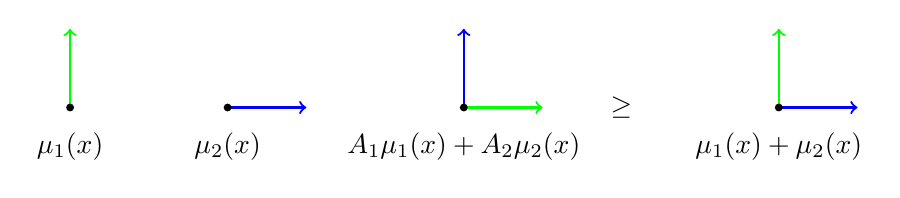
\begin{tikzpicture}
      \begin{scope}[shift={(-7,0)}]
        \draw[thick,->,green] (0,0) to (0,1);
        \fill (0,0) circle(.05);
        \node at (0,-.5) {$\mu_1(x)$};
      \end{scope}

      \begin{scope}[shift={(-5,0)}]
        \draw[thick,->,blue] (0,0) to (1,0);
        \fill (0,0) circle(.05);
        \node at (0,-.5) {$\mu_2(x)$};
      \end{scope}

      \begin{scope}[shift={(-2,0)}]
        \draw[thick,->,green] (0,0) to (1,0);
        \draw[thick,->,blue] (0,0) to (0,1);
        \fill (0,0) circle(.05);
        \node at (0,-.5) {$\pushf{A_{1}}{\mu_1(x)} + \pushf{A_{2}}{\mu_2(x)}$};
      \end{scope}

      \begin{scope}[shift={(0,0)}]
        \node at (0,0) {$\geq$};
      \end{scope}

      \begin{scope}[shift={(2,0)}]
        \draw[thick,->,green] (0,0) to (0,1);
        \draw[thick,->,blue] (0,0) to (1,0);
        \fill (0,0) circle(.05);
        \node at (0,-.5) {$\mu_1(x) + \mu_2(x)$};
      \end{scope}
    \end{tikzpicture}
    \caption{A representation of the optimal dual solution of \exemref{simple0} with the constraint \eqref{eq:dualinf1}.}
    \label{fig:simple0}
  \end{figure}

  A dual solution $\mu_1$ (resp. $\mu_2$)\footnote{In the arbitrary switching case, we write $\mu_\sigma$ instead of $\mu_{uv\sigma}$ for short}
  for the first (resp. second) matrix has the measure $\mu_1 = \delta_{(0,1)}/2$ (resp. $\mu_2 = \delta_{(1,0)}/2$).
  This is the solution obtained by applying \lemref{traj2meas} to the cycle $(1, 2)$.
  This is shown in \figref{simple0}.

\end{myexem}

\begin{myrem}
  Occupation measures for continuous switched systems are studied in \cite{claeys2016modal}.
  These measures are supported on the cartesian product of the state space and a finite interval of time $t \in [0, T]$
  while in this section, the measures are only supported on the subset $\Sn$ of the state space.
  Indeed, since the system \eqref{eq:switchsys} is homogeneous and time-invariant, we can encode trajectories in a measure on $\Sn$ (\lemref{traj2meas}) and
  still be able to recover it (\cororef{instabcert}).

  The measures studied in \cite{hare2011explicit} are supported on the paths in $\G$.
  They are related to the measures studied in this section since given a cycle $c$,
  we can compute the occupation measures of the trajectory using this switching cycle and starting with a leading eigenvector of $A_c$ as $x_0$ with \lemref{traj2meas}.
\end{myrem}



One may wonder whether \lemref{traj2meas} also works in the reverse direction to give a \emph{constructive} proof for \cororef{instabcert} when the measures $\mu_{uv\sigma}$ are atomic.
Namely, can we extract a periodic trajectory of period $c$ with $\jsrc \geq \gamlb$ from any atomic feasible solution of \progref{dualinf} with $\gamlb$.
As such solution may be the convex hull of solutions obtained by the construction of \lemref{traj2meas}, we may recover several periodic trajectory, from which there might be only one that satisfies $\jsrc \geq \gamlb$.
The following Lemma provides a constructive way to recover a periodic trajectory of period $c$ satisfying $\jsrc \geq \gamlb$ in the scalar case%
\footnote{Note that in this case, any measure is atomic since $\Sn$ is zero-dimensional}%
, i.e. $n = 1$%





\begin{mylem}
  \label{lem:instabcerts}
  Consider \defAGs{}.
  If there exists a feasible solution $\mu$ of \progref{dualinf} with $\gamlb$,
  then there exists a cycle $c$ with $\jsrc \geq \gamlb$.
  \begin{proof}
    Let $(\mu, \gamma)$ be the solution.
    By \eqref{eq:dualinf3} and \eqref{eq:dualinf1}, we can find a cycle $c$ for which each edge $e$ has a nonzero measure $\mu_e$.

    If $\jsrc \geq \gamma$, we are done.
    Otherwise, if $\jsrc < \gamma$, using \lemref{traj2meas},
    we can build a feasible solution $\nu$ such that \eqref{eq:dualinf1} is satisfied with equality for $\gamlb = \jsrc$.
    This means that $\mu - \lambda \nu$ is feasible with $\gamma$ for any $\lambda \geq 0$ such that $\mu - \lambda \nu \geq 0$.
    Let $\opt{\lambda}$ be the maximum value of $\lambda$ such that $\mu - \lambda \nu \geq 0$.
    Since $n = 1$, $\Sn$ is zero dimensional so for at least one edge $e$ of the cycle $c$, $\mu_e - \opt{\lambda} \nu_e$ is zero.
    Moreover, since $\mu_e$ is nonzero for all edge $e$ of the cycle, $\lambda > 0$.
    Therefore, the number of edges with nonzero measure has decreased and at least one of the constraints \eqref{eq:dualinf1} is now satisfied with strict inequality.

    This process can only be repeated finitely many times until $\mu$ becomes the trivial solution since the number of edges with nonzero measure decrease each time.
    Moreover we will have $\jsrc \geq \gamma$ at least once since the constraints \eqref{eq:dualinf1} cannot be satisfied with strict inequality for the trivial solution.
  \end{proof}
\end{mylem}

Given a feasible solution of \progref{dualinf} and a common partition of the support of the measures,
we show in \propref{Bsc} how to transform the solution into a solution of a scalar switched system.
Using this transformation, we can always recover a cycle $c$ for which $\jsrc = \gamma$ from a solution of \progref{dualinf} with $\gamlb = \gamma$ for which the measures are atomic.

\begin{myprop}
  \label{prop:Bsc}
  Consider \defAGe.
  Suppose that there exists a feasible solution $\mu$ of \progref{dualinf} with $\gamlb = \gamma$
  and a finite family $\mathcal{S}$ of disjoint subsets of $\Sn$ such that
  the support of each measure is included in the union of the sets of the family $\mathcal{S}$.
  Then there exists sets $B_1, \ldots, B_k \in \mathcal{S}$ and a cycle $\sigma_1, \ldots, \sigma_k$ of $\G$ such that
  \[ \prod_{i=1}^k \max_{x \in B_i} \|A_{\sigma_i} x\|_2 \geq \gamma^k \]
  and $A_{\sigma_i} B_i \cap B_{i+1} \neq \emptyset$ for $i=1, \ldots, k$ where $B_{k+1}=B_1$.
  \begin{proof}
    Given a set $B \in \mathcal{S}$ and an \arc{} $e \in \Arcs$, let $\mu_e^B$ denote the measure defined as $\mu_e^B(C) = \mu_e(C \cap B)$.
    We consider a new constrained switched system with matrices $\A' \subseteq \R^{1 \times 1}$ and automaton $\G'(\Nodes', \Arcs')$
    where $\Nodes' = \{\, (v,B) \mid v \in \Nodes, B \in \mathcal{S} \,\}$,
    $e'((u,v,\sigma), B, C) = ((u,B), (v,C), (\sigma,B))$,
    $\Arcs' = \{ e'(e, B, C) \mid e \in \Arcs, B, C \in \mathcal{S}, A_e B \cap C \neq \emptyset \}$,
    and $A'_{(\sigma,B)} = \max_{x \in B} \|A_\sigma x\|_2$.
    From any solution $\mu$ of the original system feasible for $\gamlb$, the following solution of the system with matrices $\A'$ and automaton $\G'$
    \[ \mu'_{e'(e,B,C)} = \frac{(\pushf{A_e}{\mu_e^B})(C)}{(\pushf{A_e}{\mu_e^B})(\Sn)} \mu_e(B) \]
    is also feasible with $\gamlb$.
    Indeed, by construction, for any $v \in \Nodes, C \in \mathcal{S}$, we have
    \begin{align}
        \label{eq:lhstransfer}
        \begin{split}
        \sum_{e \in \Arcsin_{1}(v), B \in \mathcal{S}} (\pushf{A_e}{\mu_e^B})(C)
        & =
        \sum_{e \in \Arcsin_{1}(v), B \in \mathcal{S}} \mu_{e'(e, B, C)}' \frac{(\pushf{A_e}{\mu_e^B})(\Sn)}{\mu_e(B)}\\
        & \stackrel{\eqref{eq:pushfineq}}{\leq}
        \sum_{e \in \Arcsin[\Arcs']_1(v, C)} \pushf{A'_{e}}{\mu_{e}'}
        \end{split}\\
        \label{eq:rhstransfer}
        \begin{split}
        \sum_{e \in \Arcsout_1(v)} \mu_e(C)
        & =
        \sum_{e \in \Arcsout_1(v), D \in \mathcal{S}} \frac{(\pushf{A_e}{\mu_e^C})(D)}{(\pushf{A_e}{\mu_e^C})(\Sn)} \mu_e(C)\\
        & =
        \sum_{e \in \Arcsout[\Arcs']_1(v, C)} \mu_{e}'.
        \end{split}
    \end{align}
    By \eqref{eq:dualinf1} on $\mu$, the left-hand side of \eqref{eq:rhstransfer} is smaller than
    the left-hand side of \eqref{eq:lhstransfer}.
    Therefore, the right-hand side of \eqref{eq:rhstransfer} is smaller than the right-hand side of \eqref{eq:lhstransfer}
    hence $\mu'$ satisfies \eqref{eq:dualinf1} on the new switched system.

    Therefore, by \lemref{instabcerts},
    there is a cycle $(\sigma_1, B_1), \ldots, (\sigma_k, B_k)$ of $\G'$ such that the modes $\sigma_i$ and sets $B_i$ are as required.
  \end{proof}
\end{myprop}

\begin{myexem}
  \label{exem:simple05}
  Consider the dual solution obtained in \exemref{simple0}.

  The supports of $\mu_1$ and $\mu_2$ are respectively $B_1 = \{(0, 1)\}$ and $B_2 = \{(1, 0)\}$.
  The automaton $G'(V', E')$ obtained by the transformation of \propref{Bsc} is defined by
  $V' = \{(1, B_1), (1, B_2)\}$ and $E' = \{((1, B_1), (1, B_2), (1, B_1)), ((1, B_2), (1, B_1), (2, B_2))\}$.
  The new $1 \times 1$ matrices are $A'_{(1, B_1)} = 1$ and $A'_{(2, B_2)} = 1$.

  The computation of the CJSR of this scalar system is a \emph{maximum cycle mean} problem
  as outlined in \cite{ahmadi2012joint}.
  The cycle of maximum geometric mean is $((1, B_1), (2, B_2))$ which geometric mean $\sqrt{1 \cdot 1} = 1$.
  We recover the cycle $(1, 2)$ found in \exemref{simple0}.
\end{myexem}

\subsection{Dual SOS program}
\label{sec:dual}
In \secref{sosswitch}, we introduced the SOS restriction of \progref{primalinf} with \progref{primal}.
In \secref{dual}, we introduce \progref{dual}, the moment relaxation of \progref{dualinf}.
It turns out that \progref{primal} and \progref{dual} are dual to each other.
Indeed, the proof of \lemref{duality} can be translated verbatim in order to prove that \progref{dual} is the dual of \progref{primal}.

\begin{myprog}[Dual of \progref{primal}]
  \label{prog:dual}

  \emph{Input}: A finite set of matrices $\A$ and an automaton $\G$.

  \emph{Output}: Pseudo-measures $\pmu_{uv\sigma}$ and a number $\gamlb$.
  \begin{align}
    \notag
    \sup_{\pmu_{uv\sigma} \in \Rhd, \gamlb \in \R} \gamlb\\
    \label{eq:dual1}
    \text{subject to }\sum_{(u,v,\sigma) \in \Arcs} \pushf{A_\sigma}{\pmu_{uv\sigma}} - \gamlb^{2d} \sum_{(v,w,\sigma) \in \Arcs} \pmu_{vw\sigma} & \in \Soshd, \quad \forall v \in \Nodes,\\
    \label{eq:dual2}
    \pmu_{uv\sigma} & \in \Soshd, \quad \forall (u,v,\sigma) \in \Arcs,\\
    \label{eq:dual3}
    \sum_{(u,v,\sigma) \in \Arcs} \pmu_{uv\sigma}(\Sn) & = 1.
  \end{align}
\end{myprog}

It is important to note that a solution of \progref{dual} is not necessarily a solution of \progref{dualinf}.
First $\pmu_{uv\sigma}$ may not be a measure even if it belongs to $\Soshd$ as discussed in \secref{moments}.
Second, the left-hand side of \eqref{eq:dual1} may also not be a measure.
For this second concern, it helps to be more explicit.
Suppose for instance that we are in the quadratic case, i.e. $d = 1$.
In that case, if $\pmu \in \Soshd[2]$, there always exists a measure $\mu$ that has the moments of the pseudo-measure $\pmu$.
We can take for instance a Gaussian distribution with these second order moments.
Hence we can find Gaussian distributions $\mu_{uv\sigma}$ that have the second order moments $\pmu_{uv\sigma}$
and Gaussian distributions $\nu_v$ that have the second order moments given by the left-hand side of \eqref{eq:dual1}.
However, we may have
\[ \sum_{(u,v,\sigma) \in \Arcs} \pushf{A_\sigma}{\mu_{uv\sigma}} - \gamlb^{2d} \sum_{(v,w,\sigma) \in \Arcs} \mu_{vw\sigma} \neq \nu_v \]
as we only know that the left-hand side and right-hand side of the above equation have the same second order moments;
see \exemref{run3}.

However, in some cases, we can recover a feasible solution of \progref{dualinf} from a feasible solution of \progref{dual}.
In these cases, by \cororef{instabcert}, this provides a lower bound on the CJSR.
Moreover, there exist efficient techniques allowing to detect situations where the solution is moments of an atomic measure; see \cite{henrion2005detecting, laurent2009sums}.
Then, using the transformation of \propref{Bsc}, we can transform
these atomic measures into a feasible solution of a constrained scalar switched systems.
For such system, we could use the algorithm described in \lemref{instabcerts} but as pointed out in \cite{ahmadi2012joint},
computing the CJSR of a scalar system can easily be done by solving a maximum cycle mean problem for which efficient algorithm exists \cite{karp1978characterization}.

If we recover a feasible solution of \progref{dualinf} from a feasible solution of \progref{dual} with $\gamlb = \jsrsos$,
we can directly conclude that $\jsrsos = \cjsr$.
This is somewhat similar to the minimization of a multivariate polynomial using SOS where we can detect that we have reached the optimum
when the measure is atomic and recover the minimizers of the polynomial from the atoms of the measure. %

However, we may also check for atomic feasible solutions of \progref{dualinf} with $\gamlb < \jsrsos$ to provide lower bounds.
Moreover, in practice, $\jsrsos$ is computed by binary search on $\gamlb$ so we often have several such solutions.

\begin{myexem}
  \label{exem:simple2}
  Consider \exemref{simple1}.
  For $i = 1, 2, 3$, let $\pmu_i$ be the solution of \progref{dual} corresponding to the matrix $A_i$.
  For any $d$, we can see that the dual solution for $\gamma = 1$ is such that
  the only monomial $x^\alpha$ such that $\la\pmu_1, x^\alpha \ra$ (resp. $\la \pmu_2, x^\alpha \ra$, $\la \pmu_3, x^\alpha \ra$) is non-zero is $x_1^{2d}$ (resp. $x_2^{2d}$, $x_3^{2d}$)
  and $\la \pmu_1, x_1^{2d} \ra = \la \pmu_2, x_2^{2d} \ra = \la \pmu_3, x_3^{2d} \ra = 1/3$.
  Note that it means that $\pmu_1 = \delta_{(1,0,0)}/3$, $\pmu_2 = \delta_{(0,1,0)}/3$ and $\pmu_3 = \delta_{(0,0,1)}/3$
  where $\delta_x$ is the Dirac measure centered on $x$.
  Since these measures are solution to \progref{dualinf} with $\gamlb = 1$,
  by \cororef{instabcert}, this means that $\jsr \geq 1$.
\end{myexem}

\begin{myexem}
  \label{exem:ando}
  We consider \cite[Example~2.8]{parrilo2008approximation}:
  \begin{align*}
    A_1 & =
    \begin{pmatrix}
      1 & 0\\
      1 & 0
    \end{pmatrix} &
    A_2 & =
    \begin{pmatrix}
      0 & 1\\
      0 & -1
    \end{pmatrix}.
  \end{align*}
  to illustrate the fact that this atom extraction pocedure can be used to determine
  when the upper bound found by \progref{primal} is equal to the CJSR.
  In this unconstrained example, the JSR is one but the upper bound found by \progref{primal} for $d=1$ is $\sqrt{2}$.
  However, for $d=2$, the upper bound found is 1 and the solutions of \progref{dual} for $\gamma=1$ is
  \begin{align*}
    \mu_1 & = 0.59698 \delta_{(1, 1)} + 0.59513 \delta_{(1, -1)} &
    \mu_2 & = 0.59513 \delta_{(1, 1)} + 0.59322 \delta_{(1, -1)}.
  \end{align*}
  Since $\pushf{A_1}{\delta_{(1, 1)}} = \delta_{(1, 1)}$, the cycle extraction method immediately find the cycle $c = 1$ for which $\rho(A_c) = 1$.
\end{myexem}

\begin{myexem}
  \label{exem:run3}
  We continue the running example; see \exemref{run1} and \exemref{run2}.

  For all $d$, $\pmu_{212} = \pmu_{323} = \pmu_{344} = \pmu_{431} = 0$
  hence the node 4 is ``unused'' by the dual.
  For $2d = 2, 4$, $\pmu_{123} = \pmu_{231} = 0$ so
  the node $2$ is ``unused'' for low degree.

  At first, one could think that the dual variables can be used to reduce the systems,
  e.g. remove nodes or edges.
  However, it would be a mistake to remove the node 2 since the periodic trajectory with highest growth rate uses this node.



  It is also interesting to notice that the matrices corresponding to the dual variables have low rank.
  For example, for $2d = 2$, $\pmu_{131}$
  (resp. $\pmu_{312}$, $\pmu_{331}$) is the Dirac measure $5.873 \cdot \delta_{(0.917,0.399)}$
  (resp. $3.966 \cdot \delta_{(0.875,0.485)}$, $6.704 \cdot \delta_{(0.757,-0.653)}$).
  However, this is not a feasible solution of \progref{dualinf}.
  Indeed,
  while \eqref{eq:dualinf1} is satisfied for \node{} 1 since
  $\pushf{A_2}{\delta_{(0.875,0.485)}}$ gives $\delta_{(0.917,0.399)}$,
  \eqref{eq:dualinf1} is not satisfied for \node{} 3 as
  $\pushf{A_1}{\delta_{(0.917,0.399)}}$ gives $\delta_{(0.999, -0.0271)}$ and
  $\pushf{A_1}{\delta_{(0.757,-0.653)}}$ gives $\delta_{(0.422, -0.906)}$.
\end{myexem}

\subsection{Constructing high growth sequence}
\label{sec:algo}
In this section we give an algorithm that generates an infinite
sequence of matrices such that the asymptotic growth rate of the
product of the matrices is arbitrarily close to the CJSR.
Note that by \defref{cjsr}, this asymptotic growth rate must be
smaller than the CJSR.


Given an \arc{} $e \in \Arcs$, let $\pE_e[p(x)] = \la \pmu_e, p(x) \ra$.
Given a polynomial $p_0(x) \in \inte(\Sosh)$ and an initial edge $(v_0,v_{-1},\sigma_0)$,
the algorithm builds a $\G^\Tr$-admissible
sequence $(v_1,v_0,\sigma_1),\allowbreak(v_2,v_1,\sigma_2), \ldots$ such that
\begin{equation}
	\label{eq:thetak}
  \theta_k \eqdef \pE_{v_{k}v_{k-1}\sigma_k}[p_0(A_{\sigma_1} \cdots A_{\sigma_k}x)]
\end{equation}
remains ``large'' for increasing $k$.
As we will see, using \lemref{thetatoA},
this implies that $A_{\sigma_1} \cdots A_{\sigma_k}$ has a ``large'' norm.

\begin{mylem}
  \label{lem:svd}
  For any matrix $A \in \R^{n \times n}$ and symmetric positive semidefinite matrix $Q$,
  the following inequality holds
  \[ \rho(A^\Tr QA) \leq \rho(Q) \rho(A^\Tr A). \]
  \begin{proof}
    Since $Q$ is symmetric positive semidefinite,
    it has a Cholesky decomposition $Q = R^\Tr R$.
    Therefore we have
    \begin{equation*}
      \rho(A^\Tr Q A) = \rho (A^\Tr R^\Tr R A)%
      = \|R A\|^2 \leq \|R\|^2 \|A\|^2 = \rho(Q) \rho(A^\Tr A).
    \end{equation*}
  \end{proof}
\end{mylem}

\begin{mylem}[{\cite[Lemma~6]{legat2016generating}}]
  \label{lem:sosbound}
  For any polynomial $p(x) \in \inte(\Sosh)$,
  there exists a constant $\beta > 0$
  such that for any matrix $A$,
  \[ \beta\|A\|_2^{2d} p(x) - p(Ax) \quad \text{is SOS} \]
  where $\|A\|_2 = \rho(A^\Tr A)^{1/2}$ is the Euclidean norm.
  Moreover we can choose $\beta = \kappa(Q)$ where $Q \in \Psd[{n+d \choose d}]$
  is a symmetric matrix such that $p(x) = (\ld{x})^\Tr Q \ld{x}$ for all $x \in \R^n$ %
  and $\kappa(Q) = \rho(Q) \rho(Q^{-1})$ is the condition number of $Q$.
  \begin{proof}
    Consider the matrix $Q$ defined in the statement of the lemma.
    Note that since $p(x) \in \inte(\Sosh)$, a positive definite $Q$ such that $p(x) = (\ld{x})^\Tr Q \ld{x}$ exists.
    We can see that
    \[ ((Ax)^{[d]})^\Tr Q(Ax)^{[d]} = (\ld{x})^\Tr (A^{[d]})^\Tr Q\ld{A}\ld{x}. \]
    Moreover, for all $x \in \R^n$,
    \[ (\ld{x})^\Tr Q\ld{x} \geq \|\ld{x}\|_2/\rho(Q^{-1}) \]
    and by \lemref{svd},
    \[ (\ld{x})^\Tr (A^{[d]})^\Tr Q\ld{A}\ld{x} \leq \rho(Q)\rho((\ld{A})^\Tr \ld{A})\|\ld{x}\|_2. \]
    Using the fact that $\rho(A^{[d]}) = \rho(A)^d$ and $(AB)^{[d]} = A^{[d]}B^{[d]}$ for any matrix $A$ and $B$,
    we have
    \[ \kappa(Q) \rho(A^\Tr A)^{d} Q - (A^{[d]})^\Tr QA^{[d]} \succeq 0. \]
  \end{proof}
\end{mylem}

\begin{mylem}
  \label{lem:thetatoA}
  Let us consider a solution $(\, \pmu_e : e \in \Arcs \,)$ of \progref{dual}.
  For any polynomial $p(x) \in \inte(\Sosh)$,
  there exists a positive constant $\tau$
  such that for any matrix $A \in \R^{n \times n}$ and \arc{} $e \in \Arcs$,
  \[ \pE_e[p(A x)] \leq \tau \|A\|_2^{2d} \]
  \begin{proof}
    If all pseudo-expectations are zero, the result is trivially true.
    Therefore we can suppose that at least one is nonzero.
    By \lemref{sosbound}, there exists a constant $\beta > 0$ such that
    \[ \beta \|A\|_2^{2d}p(x) - p(Ax) \text{ is SOS}. \]
      Hence for any \arc{} $e \in \Arcs$,
    \[
      \pE_e[p(Ax)] \leq \beta \|A\|_2^{2d} \pE_e[p(x)].
    \]
    We obtain the result with the constant
    \(
    \tau = \beta \max_{e \in \Arcs} \pE_{e}[p(x)].
    \)
    Since at least one pseudo-expectation is nonzero and $p(x)$ is in
    the interior of the SOS cone, $\tau > 0$.
  \end{proof}
\end{mylem}


\begin{algorithm}[!ht]
  \caption{Generates a sequence of large asymptotic growth.}
  \label{algo:prodl}
  \begin{algorithmic}
    \STATE{\textbf{Data}: Length of subpaths: $l \in \mathbb{N}$; degree: $d \in \mathbb{N}$; and lower bound to $\jsrsos$: $0 < \gamma < \jsrsos$.}
    \STATE{\textbf{Result}: Sequence of arbitrary length $s = (\ldots, v_{k},\sigma_{k},\ldots,v_0,\sigma_{0},v_{-1})$.}
    \STATE{Given a feasible solution $(\, \pmu_e : e \in \Arcs \,)$ of \progref{dual} with $\gamlb = \gamma$ and degree $d$}
    \STATE{Pick an arbitrary polynomial $p_0(x) \in \inte(\Sosh)$}
    \STATE{Pick an \arc{} $(v_0,v_{-1},\sigma_0) \in \Arcs$ such that $\pmu_{v_0v_{-1}\sigma_0}$ is nonzero}
    \FOR{$k = 0,l,2l,\ldots$}
    \STATE Pick $s \in \argmax_{s \in \Arcsin_l(v_{k})} \pE_{s[1]}[p_k(A_s x)]$
    \STATE Set $(v_{k+l},\sigma_{k+l},\ldots,\sigma_{k+1},v_k) \leftarrow s$
    \STATE Set $p_{k+l} \leftarrow p_k(A_s x)$
    \ENDFOR
  \end{algorithmic}
\end{algorithm}




\lemref{maxdegpathl} provides a guarantee on the growth rate of $\theta_k$, defined in \eqref{eq:thetak},
using the dual constraint~\eqref{eq:dual1}.

\begin{mylem}
  \label{lem:dualconsl}
  Given \defAG{}, %
  if $\pmu$ is a feasible solution of \progref{dual} then,
  for any edge $(\bar{u},\bar{v},\bar{\sigma}) \in \Arcs$,
  the following holds:
  \begin{equation}
    \label{eq:dualconsl}
    \sum_{s \in \Arcsin_k(\bar{u})} \pushf{A_s}{\pmu_{s[1]}} \succeq \gamma^{2dk} \pmu_{\bar{u}\bar{v}\bar{\sigma}}
  \end{equation}
  where $\pmu_1 \succeq \pmu_2$ denotes $\pmu_1 - \pmu_2 \in \Soshd$.
  \begin{proof}
    We prove \eqref{eq:dualconsl} by induction, the case of $k=0$ being trivial.
    Suppose that
    \begin{equation}
      \label{eq:indhyp}
      \sum_{s' \in \Arcsin_{k-1}(\bar{u})}\pushf{A_{s'}}{\pmu_{s'[1]}} \succeq \gamma^{2d(k-1)} \pmu_{\bar{u}\bar{v}\bar{\sigma}}.
    \end{equation}
    We can rewrite the left-hand side of \eqref{eq:dualconsl} as
    \begin{equation}
      \label{eq:splitdualconsl}
      \sum_{s \in \Arcsin_k(\bar{u})} \pushf{A_s}{\pmu_{s[1]}} = \sum_{s' \in \Arcsin_{k-1}(\bar{u})} \pushf{A_{s'}}{\sum_{(u,s'(1),\sigma) \in \Arcs} \pushf{A_\sigma}{\pmu_{us'(1)\sigma}}}.
    \end{equation}
    By \eqref{eq:dual1},
    \[
      \sum_{(u,s'(1),\sigma) \in \Arcs} \pushf{A_{\sigma}}{\pmu_{us'(1)\sigma}}
      \succeq \gamma^{2d} \sum_{(s'(1),w,\sigma') \in \Arcs} \pmu_{s'(1)w\sigma'}.
    \]
    Since the dual variables $\pmu_{s'(1)w\sigma'}$ of the right-hand side are in the dual of the SOS cone,
    and one of them is $\pmu_{s'[1]}$, we have
    \[
      \sum_{(u,s'(1),\sigma) \in \Arcs} \pushf{A_{\sigma}}{\pmu_{us'(1)\sigma}}
      \succeq \gamma^{2d} \pmu_{s'[1]}.
    \]
    Applying $\pushf{A_{s'}}{}$ on both sides and using \eqref{eq:splitdualconsl} gives
    \[
      \sum_{s \in \Arcsin_k(\bar{u})} \pushf{A_s}{\pmu_{s[1]}} \succeq \gamma^{2d} \sum_{s' \in \Arcsin_{k-1}(\bar{u})}\pushf{A_{s'}}{\pmu_{s'[1]}} \stackrel{\eqref{eq:indhyp}}{\succeq} \gamma^{2dk} \pmu_{\bar{u}\bar{v}\bar{\sigma}}.
    \]
  \end{proof}
\end{mylem}

\begin{mylem}
  \label{lem:maxdegpathl}
  Consider \defAGe{}.
  For any positive integers $d$ and $l$,
    using \progref{dual} with any $\gamma < \jsrsosa\\(\G,\A)$,
  \algoref{prodl} with paths of length $l$
  produces a $\G^\Tr$-admissible sequence
  $(v_1,v_0,\\\sigma_0),(v_2,v_1,\sigma_1), \ldots$ %
  for which the sequence of $\theta_k$ defined in \eqref{eq:thetak}
  satisfies the following inequality for all $k > 0$ multiple of $l$:
  \begin{equation*}
    \theta_{k}
    \geq \frac{\gamma^{2dl}}{\dink[l](v_{k-l+1})}
    \theta_{k-l}
  \end{equation*}
  \begin{proof}
    By \lemref{dualconsl},
    \begin{align*}
      \sum_{s \in \Arcsin_l(v_{k-l+1})} \pE_{s[1]}[p_{k-l}(A_s x)]
      & \geq \gamma^{2dl} \theta_{k-l}.
    \end{align*}
    Since the value of $s$ chosen by \algoref{prodl} maximises $\pE_{s[1]}[p_{k-l}(A_s x)]$,
    the left-hand side of the above inequality is smaller or equal to $\dink[l](v_{k-l+1})\theta_k$.
  \end{proof}
\end{mylem}

\theoref{fourth} translates the guarantee on $\theta_k$ to a guarantee on $A_{\sigma_1} \cdots A_{\sigma_k}$ using \lemref{thetatoA}.

\begin{mytheo}
  \label{theo:fourth}
  Consider \defAGe{}.
  For any positive integers $d$, $l$ and
  a lower bound $\gamma < \jsrsos$,
  \algoref{prodl} with input $l, d$ and $\gamma$
  produces a $\G^\Tr$-admissible sequence
  $(v_1,v_0,\sigma_0), (v_2,v_1,\sigma_1), \ldots$ %
  that satisfies the following inequality:
  \begin{equation*}
    \lim_{k \to \infty} \|A_{s_k}\|_2^\frac{1}{k} \geq \frac{\gamma}{(\mdin_l(\G))^\frac{1}{2dl}}
  \end{equation*}
  where $s_k = (\sigma_k, \ldots, \sigma_1)$.
  \begin{proof}
    By \lemref{maxdegpathl}, for any $k$ multiple of $l$, %
    \begin{equation*}
      \pE_{s_k[1]}[p_0(A_{s_k}x)] \geq \frac{\gamma^{2dk}}{(\mdin_l(\G))^\frac{k}{l}} \pE_{v_0v_{-1}\sigma_0}[p_0(x)]
    \end{equation*}

    By Lemma~\ref{lem:thetatoA},
    there exists a constant $\tau > 0$ such that
    \[
      \pE_{s_k[1]}[p_0(A_{s_k} x)] \leq \tau \|A_{s_k}\|^{2d}.
    \]

    Combining these two inequalities, we obtain
    \begin{align*}
      \tau \|A_{s_k}\|^{2d} & \geq \frac{\gamma^{2dk}}{(\mdin_l(\G))^\frac{k}{l}} \pE_{v_0v_{-1}\sigma_0}[p_0(x)].
    \end{align*}
    Since $\pE_{v_0v_{-1}\sigma_0}$ is nonzero, $\pE_{v_0v_{-1}\sigma_0}[p_0(x)] > 0$.
    Therefore taking the $(2dk)$th root and the limit $k \to \infty$
    we obtain the result.
  \end{proof}
\end{mytheo}




\begin{myexem}
  \label{exem:simple3}
  Suppose that we apply Algorithm~\ref{algo:prodl} with $l = 1$ to \exemref{simple2}
  and let us denote by $c_\alpha$ the coefficient of the monomial $x^\alpha$ in the polynomial $p_0(x)$ chosen arbitrarily by the algorihtm.
  The start of the sequence produced depends on the order between
  the coefficients $c_{(2d,0,0)},\allowbreak c_{(0,2d,0)},\allowbreak c_{(0,0,2d)}$.
  If $c_{(2d,0,0)}$ is the largest then
  the $\G$-admissible left-infinite sequence found is
  \( \ldots,1,2,3,1,2,3,1,2,3. \)

  The product $A_{\sigma_1} A_{\sigma_2} A_{\sigma_3} \cdots = A_3A_2A_1A_3A_2A_1 \cdots $
  is periodic and has an asymptotic growth rate $\rho(A_{\sigma_1}A_{\sigma_2}A_{\sigma_3})^{1/3}\allowbreak = 1$.
  Hence $1 \leq \cjsr$.
\end{myexem}


\subsection{Deducing a lower bound certificate}
\label{sec:lb}


By definition of the CJSR, the asymptotic growth rate of the norm of the product of any $\G$-admissible (or $\G^\Tr $-admissible) sequence of matrices gives a lower bound on the CJSR.
In particular the sequence produced by Algorithm~\ref{algo:prodl} provides a lower bound on the CJSR.

If there are two integers $\bar{k},k$ such that the sequence after $\bar{k}$ is periodic of period $k$,
the asymptotic growth rate of the norm is equal to the $k$th root of the spectral radius of the product of the matrices of one period.
This is due to the Gelfand's formula $\rho(A) = \lim_{k \to \infty} \|A^k\|^{1/k}$.
From the same identity,
we see that the spectral radius of the product of the matrices of one $\G$-admissible cycle gives a lower bound on the CJSR.



To find lower bounds for the CJSR,
one could generate all the cycles of length smaller than some maximum length
and compute the spectral radius for all of them.
This brute force approach is not scalable because the number of paths considered grows exponentially with the maximum length.%
\footnote{The exponential growth of the brute force approach is the reason why one should choose a small $l$ for Algorithm~\ref{algo:prodl}.}

Gripenberg~\cite{gripenberg1996computing} proposes a branch-and-bound algorithm that prunes the search using an a priori fixed absolute error.
Other alternative methods exist such as
the balanced complex polytope algorithm \cite{guglielmi2008algorithm, guglielmi2013exact}
and the invariant conitope algorithm~\cite{jungers2014lifted}.
The methods attempts to generate an invariant polytope from the eigenvector
of a cycle of high growth rate.
A candidate of cycle of higher growth rate can be found while constructing this polytope,
the construction is then restarted with its eigenvector as a new stating point.
While computing this polytope, convexity arguments allows to prune paths
which attenuate the exponential growth of the number of paths.
Specialized methods exist for some particular matrix structures
such as the ``spectral simplex method'' \cite{protasov2016spectral}
in the case of nonnegative matrices with a ``product structure''.

These algorithms can also be used to produce a $\G$-admissible sequence of matrices of high asymptotic growth rate
by reproducing the cycles of high spectral radius infinitely.
The advantage of \algoref{prodl} is that it provides a guarantee of accuracy given in \theoref{fourth}.
\algoref{prodl} provides at the same time a high growth infinite trajectory and lower bounds of guaranteed accuracy.

\algoref{prodl} requires to solve a semidefinite program with semidefinite
matrices of size ${n + d - 1 \choose d}$.
Then, in order to add $l$ new edges to the sequence,
it needs to go through $\mdin_l(\G)$ paths and compare them by computing the scalar product
between a polynomial and moments with ${n + 2d - 1 \choose 2d}$ monomials.
The semidefinite program can be solved in a time polynomial in ${n + d - 1 \choose d}$
and $|\Arcs|$ as detailed in \secref{sdp},
and adding $l$ edges to the sequence can be done in a time proportional to $\mdin_l(\G){n + 2d - 1 \choose 2d}$.
While polytopes are used in \cite{guglielmi2008algorithm, guglielmi2013exact, jungers2014lifted}
to prune paths, \algoref{prodl} uses a solution of \progref{dual} to guide the search
which enables the discovery of sequences of guaranteed high growth rate even with a small value of $l$.
Moreover, \exemref{FinConjCounterEx} and \secref{application} %
give examples where \algoref{prodl} uncovers rather long cycles of high asymptotic growth rate.
This shows the complementarity of \algoref{prodl} with existing approaches
which performs better when the cycles of high growth rate have a small length as they
iterate over possible cycles of increasing length (although some are pruned).
Moreover, \cite{gomes2018minimally} shows that the algorithms can handle constrained switched systems with automaton of large size, as it stabilizes a system with 64 nodes and 512 edges \cite[Table I]{gomes2018minimally}.

\begin{myexem}
\label{exem:FinConjCounterEx}
We consider the switched system introduced in \cite{blondel2003elementary}
as a counterexample to the finiteness conjecture \cite{lagarias1995finiteness}.
We use the value $\alpha = 0.7493265463303675$ which is the
IEEE double-precision number %
that is closest to the value
given in \cite{hare2011explicit} for which the system does not satisfy
the finiteness property.
\tabref{FinConjHigh} gives two cycles of high growth rate;
as the reader can check, their growth rates are rather close.
We verified that there exists no cycle of length up to 32 that provides a larger lower bound.

\begin{table}
  \centering
  \begin{tabular}{|c|l|l|}
    \hline
    length & cycle & growth rate\\
    \hline
    13 & 2112112121121 & 1.4092472220583443\\
    \hline
    21 & 211211212112112121121 & 1.4092472220583487\\
    \hline
  \end{tabular}
  \caption{Two cycles of high growth rate for the switched system of \exemref{FinConjCounterEx}.}
  \label{tab:FinConjHigh}
\end{table}

\begin{figure}
  \centering
  \includegraphics[width=0.75\textwidth]{FinConjCounterEx.png}
  \caption{
    Illustration of the polysets corresponding to the
    optimal solution of \progref{primal} for \exemref{FinConjCounterEx} and for different degree $2d$.
    In the first row, from left to right, it corresponds to
    $2d = 2, 4, 6, 8, 10$.
    In the second row, from left to right, it corresponds to
    $2d = 12, 14, 16, 18, 20$.
    In the third row, from left to right, it corresponds to
    $2d = 22, 24, 26, 28, 30$.
  }
  \label{fig:FinConjCounterEx}
\end{figure}

The polysets corresponding to the optimal solution of \progref{primal}
for $2d = 2, 4, \ldots, 30$ are given in \figref{FinConjCounterEx}.
Using Algorithm~\ref{algo:prodl} with $2d=2$, $l = 4$ and $p_0$ equal to the
solution of \progref{primal}, the algorithm generates a sequence starting with
the cycle of length 21 in \tabref{FinConjHigh}.

We consider now the Balanced Polytope algorithm exploiting the nonnegativity of the matrices \cite[Section~4]{guglielmi2013exact}.
A point $p$ is considered to belong to the interior of a balanced polytope $P$ if MOSEK~\cite{mosek2017mosek81082} with its dual simplex algorithm certifies that the maximal $t$ such that $tp \in P$ is larger than $1 + \num{3e-13}$.
The algorithm first finds the cycle of length 13 in \tabref{FinConjHigh} and
is then able to find the cycle of length 21 with the tolerance \num{3e-13}.
However, if the \num{3e-13} tolerance is replaced by $\num{-1e-12}$ or lower,
then the algorithm does not find this second cycle.
This behavior is not surprising given how close the growth rates are as shown in \tabref{FinConjHigh}.

A cycle with growth rate equal to the CJSR is often called \emph{spectral maximizing product} (s.m.p.).
The algorithm is able to conclude that the cycle of length 21 is an s.m.p. with the tolerance \num{3e-13}.
If we replace the \num{3e-13} by \num{4e-13},
it does not seem to terminate as the number of leaves in the tree increases with the
depth considered.
We will consider this cycle to be an s.m.p. for the purpose of the benchmark even though
it cannot be said for certain.



\end{myexem}

We can compute ``non-constructive'' lower bounds (it is not constructive as it does not exhibit a cycle certifying the lower bound)
using the guarantee (given in \cite[Corollary~1]{legat2016generating}) on the upper bound \eqref{eq:upperbound} provided by Program~\ref{prog:primal},
but in practice the trajectories found by \algoref{prodl} are periodic after some time $\bar{k}$ so we are able to compute
much better lower bounds than the pessimistic bound provided by the guarantee.
This is shown by \exemref{run4}.

\begin{myexem}
  \label{exem:run4}
  We tried the atom extraction procedure introduced in \secref{dual} and Algorithm~\ref{algo:prodl} for $l = 1$ and $l = 3$ on our running example;
  see \exemref{run1}, \exemref{run2} and \exemref{run3}%
  . The result is shown in \figref{pedj}.
  We showed in \cite{legat2016generating} that the CJSR of the system is equal to 0.97482.
  We can see that this lower bound is found for $d = 4$ for $l=1$ and for $d=1$ for $l=3$.
  The atom extraction finds the lower bound 0.939255.
\end{myexem}

\begin{figure}[!ht]
  \begin{subfigure}{0.48\textwidth}
    \centering
    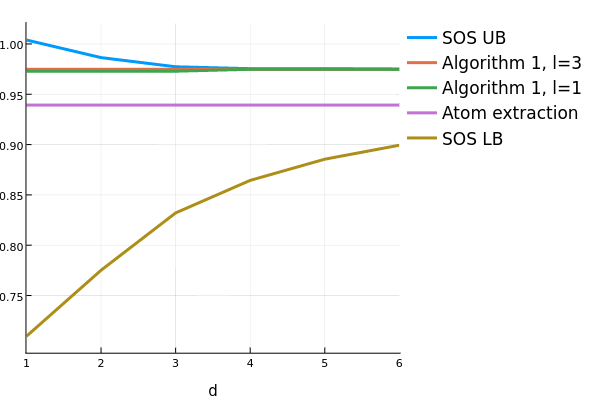
\includegraphics[width=\textwidth]{../../latex/images/PEDJ.png}
  \end{subfigure}
  \begin{subfigure}{0.48\textwidth}
    \centering
    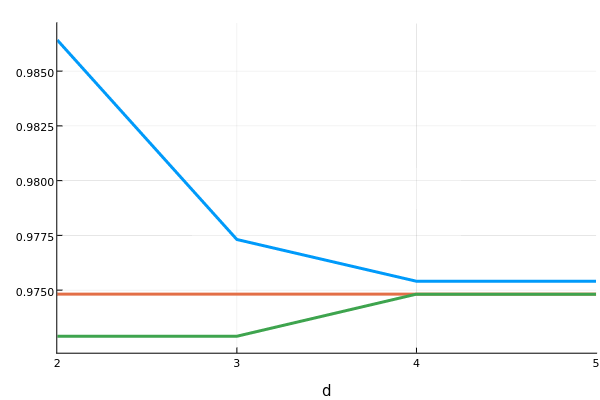
\includegraphics[width=\textwidth]{../../latex/images/PEDJ_zoom.png}
  \end{subfigure}
  \caption{Result of \exemref{run4}. The SOS UB is the upper bound found by \progref{primal} and the SOS LB is obtained from its guarantee; see \cite[Corollary~1]{legat2016generating}. The value $d$ of horizontal axis corresponds to using polynomials of degree $2d$. The right figure is a zoom of the left figure.}
  \label{fig:pedj}
\end{figure}

\begin{myexem}
  \label{exem:long_prod}
  Consider the unconstrained switched system with the following two matrices\footnote{This example was found in a previous collaboration with N. Guglielmi and A. Cicone (unpublished).}:
  \[
    A_1 = \begin{bmatrix}
      -1 &  1 & -1\\
      -1 & -1 &  1\\
       0 &  1 &  1
    \end{bmatrix} \qquad
    A_2 = \begin{bmatrix}
      -1 &  1 & -1\\
      -1 & -1 &  0\\
       0 &  1 &  1
    \end{bmatrix}.
  \]
  The s.m.p. has length 41 and growth rate $1.684185$:
  \begin{center}
    11122112211221122112211221122112211221112.
  \end{center}
\end{myexem}

We summarize in \tabref{benchlb} and \tabref{benchub} the time taken by the different methods on the examples.
As we can see in \tabref{benchlb}, the time taken by \algoref{prodl} to find the s.m.p. is competitive compared
to alternative approach once the Sum-of-Squares pair of primal-dual programs \progref{primal}/\progref{dual} has been solved.
Moreover, as we can see in \tabref{benchub}, finding upper bounds by solving this pair of programs is
competitive with alternative approaches.

\begin{table}
  \centering
  \begin{tabular}{|cc|c|c|cccc|}
    \hline
    Example                     & length & GRIP [s] & BP [s] & $d$ & $l$ & SOS [s] & SEQ [s]\\
    \hline
    \ref{exem:FinConjCounterEx} & 21 & 0.076    & 0.07  & 1   & 4   & 0.12    & 0.0013\\
                                &    &          &       & 15  & 2   & 0.80    & 0.020\\
    \hline
    \ref{exem:run4}             & 8  & 0.051    & 0.54  & 1   & 3   & 0.15    & 0.0011\\
                                &    &          &       & 4   & 1   & 0.28    & 0.0011\\
    \hline
    \ref{exem:long_prod}        & 41 & 0.040    & 5.08  & 1   & 9   & 0.14    & 0.073\\
                                &    &          &       & 4   & 2   & 0.76    & 0.074\\
    \hline
  \end{tabular}
  \caption{Comparison of the performance of different algorithms to find a s.m.p.
  The second column provides the length of the smallest s.m.p.
  GRIP is the time taken by the Gripenberg algorithm~\cite{gripenberg1996computing} to find a s.m.p.
  BP is the time taken by the Balanced Polytope algorithm~\cite{guglielmi2013exact} to
  find a s.m.p.
  The nonnegativity of the matrices is exploited for \exemref{FinConjCounterEx} as
  suggested in Section~4 of \cite{guglielmi2013exact}.
  A point $p$ is considered to belong to the interior of a balanced polytope $P$ if MOSEK~\cite{mosek2017mosek81082} certifies that the maximal $t$ such that $tp \in P$ is larger than $1 + \num{3e-13}$.
  SOS is the time taken by MOSEK~\cite{mosek2017mosek81082} to solve the pair of primal-dual programs \progref{primal}/\progref{dual} with degree $d$ using a bisection on $\gamma$ until $\log(\gamub) - \log(\gamlb) < \num{1e-2}$ where $\gamub$ is the smallest $\gamma$ such that \progref{primal} is feasible and $\gamlb$ is the largest $\gamma$ such that \progref{dual} is feasible.
  SEQ is the time taken by \algoref{prodl} with input $l, d$ and $\gamlb$.
  The timings are taken from \texttt{Benchmark.html} of \cite{5f757996-cc62-479c-86f3-eac76e3e9580}.}
  \label{tab:benchlb}
\end{table}

\begin{table}
  \centering
  \begin{tabular}{|cc|c|c|cc|}
    \hline
    Example & $\delta$ & GRIP [s] & BP [s] & $d$ & SOS [s]\\
    \hline
    \ref{exem:FinConjCounterEx} & \num{6e-4} & 1.58 & 3.038 & 7 & 0.91\\
    \hline
    \ref{exem:run4} & \num{25e-8} & 9.04 & 0.207 & 7 & 1.63\\
    \hline
    \ref{exem:long_prod} & \num{1e-3} & 0.37 & 14.273 & 6 & 8.40\\
    \hline
  \end{tabular}
  \caption{Comparison of the performance of different algorithms to find an upper bound to the CJSR.
  GRIP is the time taken by the Gripenberg algorithm~\cite{gripenberg1996computing} to
  prove the upper bound $\cjsr + \delta$.
  The timing BP differs from the timing BP in \tabref{benchlb} in the fact that we wait
  for the algorithm to prove that it is an s.m.p.
  The timing SOS differs from the timing SOS in \tabref{benchlb} only in the bisection
  stopping criterion which is $\gamub - \cjsr < \delta$ for this table.
  The timings are taken from \texttt{Benchmark.html} of \cite{5f757996-cc62-479c-86f3-eac76e3e9580}.}
  \label{tab:benchub}
\end{table}

\subsection{Conclusion}

We have analyzed the dual of the set program for polysets of degree $2d$
and shown how to leverage it to study the stability of switched system.
We gave a rounding algorithm (\algoref{prodl}) that generates from a solution of the dual program a
switching sequence of growth rate guaranteed by \theoref{fourth}.
We also showed in \propref{Bsc} that given atomic measures solution of this dual program,
we can extract a high growth-rate trajectory of the switched systems
by transforming them to the solution a scalar constraint switched systems.

We have introduced two techniques to generate lower bounds from the solution of the SOS dual program.
In practice, these techniques provide periodic trajectories of high asymptotic growth rate.
Since the SOS program can be solved efficiently,
does this give an efficient algorithm to generate lower bounds on the CJSR with \emph{guaranteed accuracy}?
This is not clear, as we have no guarantee on length of the period of the trajectory generated and whether it is even periodic. %


\section{Constrained switching stabilitization}
\label{sec:switchstab}

In this section, we are motivated by a new application \cite{Gomes2017d} in the field of co-simulation.
It is a numerical technique to couple multiple simulators, each simulating a part of a coupled system, in order to compute the overall behavior more efficiently~\cite{gomes2018co}.
We focus on the abstract problem in this section and refer the reader
to \cite{gomes2018minimally} for more details on the application to co-simulation.

We tackle the problem of how to best forbid policy sequences that make the constrained switched system unstable.
We propose that the best solution is to maximize the \emph{entropy} of the stabilized constrained switched system in order to maximize the adaptability of the resulting (co-)~simulation method.

Our goal is to optimally modify a given constrained switched system, by forbidding unstable switching signal cycles from the language it generates.
The problem of finding such cycles is considered in \secref{certifylowerbound}.
As such, we introduce the following definition, which represents any algorithm available for this purpose.
\begin{mydef}[Oracle]\label{def:oracle}
  Given $\epsilon > 0$, we define a \emph{stability oracle} $\Oracle_\epsilon: S \to \{\texttt{Stable}\} \cup \bigcup_{k=1}^\infty \Cycles$, where $S$ is a CSS.
  The oracle $\Oracle_\epsilon$ returns either \texttt{Stable} certifying that $\jsr(S) < 1$ or a cycle $c \in \Cycles$ such that $\rho(A_c)^{1/k} > 1 - \epsilon$.
\end{mydef}

We emphasize that the oracle has a (slightly) imperfect behavior: in case $1-\epsilon < \jsr(S) < 1$,
one cannot guarantee what the outcome of the oracle will be.
This imperfection is intentional%
, as it models the state of the art \cite{parrilo2008approximation}.
The result~\eqref{eq:cjsrrk} ensures that if $\jsr(S) > 1 - \epsilon$, there exists a $k$ and a cycle $c \in \Cycles$ such that $\rho(A_c)^{1/k} > 1 - \epsilon$.

We now proceed to define the set of possible different switching signals that are admissible.

\begin{mydef}[Admissible Regular Language]
  \label{def:reg}
  We say that $\Lang=\LangAutom$ is the language \emph{recognized} by the automaton $\G$.
  A language is \emph{regular} if it is recognized by a finite automaton.
  A language $\Lang$ recognized by an automaton $\G$ is \emph{admissible} for $\A$ if the constrained switched system $S = \tuple{\A, \G}$ satisfies
  $\jsr(S) < 1$.
\end{mydef}

Let $\Lang_0$ denote the language recognized by the automaton $\G_0$ of a given $S = \tuple{\A, \G_0}$.
Informally, our goal is to find the ``largest'' regular language $\opt{\Lang} \subseteq \Lang_0$ that is admissible.
For this optimization problem to be well defined we need to find a metric for the objective.
This metric should be in accordance to the fact that given $\Lang \subseteq \Lang'$, the objective should favor $\Lang'$.
A widely used notion to describe the size of a regular language is that of Entropy, defined in \defref{entropy}.

We denote the entropy of the language $\LangAutom$ recognized by an automaton $\G$ as $\LangAutom[h](\G)$.

If $\Lang \subseteq \Lang'$, then $\Paths \subseteq \Paths'$ for any $k$, and so $h(\Lang) \leq h(\Lang')$.
Our problem can now be formulated.
\begin{myprob}\label{eq:prob}
  Given a CSS $\tuple{\A, \G_0}$,
  find the language $\opt{\Lang}$ solution of the following optimization problem:
  \begin{align}
\notag
    \opt{\Lang} = \sup_{\Lang \text{ regular}} h(\Lang) \text{ s.t.}\\
\notag
    \Lang & \subseteq \Lang_0,\\
    \label{eq:admissible}
    \Lang & \text{ is admissible for }\A.
  \end{align}
  where $\Lang_0$ is the language recognized by $\G_0$.
\end{myprob}

\begin{myrem}
  In \eqref{eq:prob}, we restrict our attention to regular languages.
  While there are examples that highlight the benefit of using non-regular languages (see \exemref{pumping}),
  in practice, one needs an \emph{efficient} way of generating accepted switching signals.
	For instance, during a co-simulation, at any step, the simulators need to compute as quickly as possible the set of policies that can be taken (see \cite[Section 4.4]{Gomes2017d} for how this can be done).
  Automata allow the decision procedure to be fast, with little memory.
  In addition, as hinted in \exemref{1cycle}, regular languages may be constructed to approximate an admissible language with entropy arbitrarily close to the entropy of the optimal solution, even if that optimal solution is a non-regular language.
\end{myrem}

\begin{myexem}
  \label{exem:pumping}
  Consider $\A=\set{A_1, A_2}$, with $A_1 = 2$ and $A_2 = \frac{1}{2}$, and $\G = (V, E)$, where
  $V=\set{v_1}$ and $E = \set{ (v_1, v_1, 1), (v_1, v_1, 2)}$.
  That is, $\G$ has the form
  \begin{equation*}
  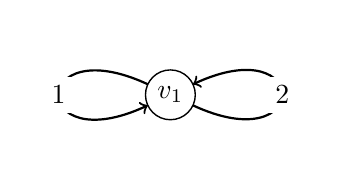
\begin{tikzpicture}
    \Vertex[L={$v_1$}]{1}
    \draw[thick,->] (1) to [out=155,in=205,looseness=16] node [midway, fill=white] {$1$} (1);
    \draw[thick,->] (1) to [out=-25,in=25,looseness=16] node [midway, fill=white] {$2$} (1);
  \end{tikzpicture}
  \end{equation*}
  The optimal solution $\opt{\Lang}$ of (relaxed) \eqref{eq:prob} should include every word that has more $1$s than $2$s.
  As shown in \cite[Example~1.73]{Sipser2013}, no automaton can be built that accepts this language.
\end{myexem}

\begin{figure}
  \centering
  \includegraphics[width=0.6\textwidth]{1cycle_custom}
  \caption{Evolution of $h(\Lang_k)$ of \exemref{1cycle} in terms of $k$.}
  \label{fig:1cycle}
\end{figure}

\begin{myexem}
  \label{exem:1cycle}
  Consider $\A=\set{A_1, A_2}$, with $A_1 = 1$ and $A_2 = \frac{1}{2}$.
  A language is admissible if it does not contain the infinite repetition of the symbol 1.
  Let $\Lang_k$ be language of all words that do not contain $k$ consecutive 1's.
  \figref{1cycle} suggests that that $h(\Lang_k)$ tends to $\log_2(2)$ when $k$ tends to infinity.
  The quantity $\log_2(2)$ denotes the entropy of the optimal solution.
\end{myexem}

\subsection{Lift-and-Constrain Stabilization}
\label{sec:stabilization_ss}

\subsubsection{Constraining for more stability}
\label{sec:constrain_for_stability}

\algoref{stabilization} details an iterative procedure that stabilizes a given CSS $S = \tuple{\A, \G}$, using the oracle in \defref{oracle}.
At each iteration, if the oracle returns a cycle $c=\sigma_k \ldots \sigma_k$, then $c$ is eliminated from $\G$.
The removal of a cycle can be accomplished by removing an edge of $\G$, thus potentially decreasing $\jsr(S)$.
After removing the cycle $c$, any infinite sequence in $\LangAutom$ for which $c$ is a subsequence will be eliminated too.
This is illustrated in \exemref{edge_removal_example}.
The algorithm can produce an empty CSS, which does not imply that the original CSS is impossible to stabilize.
An empty CSS is trivially stable.

\begin{myexem}\label{exem:edge_removal_example}
Consider the automaton in \figref{edge_removal_example}, and suppose the oracle has returned the cycle $234$.
This cycle is highlighted in red, in the figure.
Any of the edges in red can be removed to forbid the unstable sequence.
If edge $v_1 \xrightarrow{2} v_2$ is removed, the infinite sequences accepted by the resulting automaton end with either an infinite sequence of $2$'s, or an infinite sequence of $3$'s.
If edge $v_2 \xrightarrow{3} v_3$ is removed instead,
the resulting automaton accepts infinite sequences comprised of repeating subsequences which include $2$, or $3$, or $12$.
\end{myexem}

\begin{figure}[tbh]
\centering
  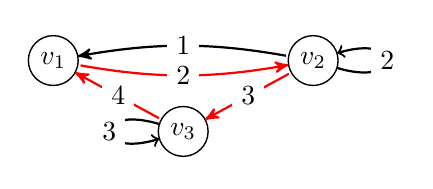
\begin{tikzpicture}[xscale=1.1,yscale=0.6]
    \Vertex[L={$v_1$}]{1}
        \EA[L=$v_2$,unit=3](1){2}
        \SOEA[L=$v_3$,unit=1.5](1){3}
        \SetUpEdge[style={post,{->}, thick},color=red]
        \Edge[label=$3$](2)(3)
        \Edge[label=$4$](3)(1)
        \SetUpEdge[style={post,bend right=18,thick},color=red]
        \Edge[label=$2$](1)(2)
        \SetUpEdge[style={post,bend right=18,thick}]
        \Edge[label=$1$](2)(1)

        \draw[thick,->] (2) to [out=-25,in=25,looseness=5] node [midway, fill=white] {$2$} (2);
        \draw[thick,->] (3) to [out=155,in=205,looseness=5] node [midway, fill=white] {$3$} (3);
  \end{tikzpicture}
  \caption{Automaton of \exemref{edge_removal_example}.}
  \label{fig:edge_removal_example}
\end{figure}

As \exemref{edge_removal_example} shows, the choice of different edges to be removed has a different impact in the entropy of the resulting automaton.
Informally, removing the edge $v_2 \xrightarrow{3} v_3$ seems to be the best choice because the resulting automata allows for \emph{more} sequences.
This is corroborated by computing the entropy of the resulting automaton alternatives.
See \secref{entropy} for how to compute the entropy in this example.


\begin{algorithm}
  \begin{algorithmic}
  \STATE{\textbf{Input} A CSS $S=\tuple{\A, \G}$.}
  \STATE{\textbf{Output} A stable CSS $S=\tuple{\A, \G}$.}
  \WHILE{$\Oracle_\epsilon(S) \neq {}$\texttt{Stable}}
	\STATE \begin{enumerate}
    \item\label{algo:stabilization:s2} Find $e \in \argmax \{\, \LangAutom[h](\G - e) \mid e \in E$, $e$ is\\an edge of the cycle $\Oracle_\epsilon(S) \,\}$\;
    \item Set $\G := \G - e$\;
	 \end{enumerate}
  \ENDWHILE
  \end{algorithmic}
   \caption{Stabilization algorithm for a constrained switched system. $\LangAutom[h](\G)$ denotes the entropy of the language recognized by $\G$. The difference $\G - e$ denotes the automaton obtained by removing the edge $e$ from $\G$.}
	 \label{algo:stabilization}
\end{algorithm}

The following result demonstrates that \algoref{stabilization} always terminates.

\begin{mytheo}\label{theo:termination}
  Given a CSS $S = \tuple{\A, \G}$ and
  an oracle satisfying \defref{oracle},
  \algoref{stabilization} terminates after finitely many iterations and the resulting CSS
  is stable.

  \begin{proof}
    At each iteration of the algorithm, the number of edges of the automaton $\G = (V, E)$ decreases by one.
    Since at the beginning of the algorithm $|E|$ is finite,
    the algorithm must terminate after a finite number of iterations.
    The condition for termination of \algoref{stabilization} implies that the resulting system is stable.
  \end{proof}
\end{mytheo}

\begin{myrem}
In \theoref{termination}, the assumption that the oracle in \defref{oracle} always terminates is crucial, as the problem solved by the oracle is undecidable in general. %
\end{myrem}

\subsubsection{Lifting for less conservativeness}

\algoref{stabilization} takes a constrained switched system $S=\tuple{\A, \G}$, and outputs a constrained switched system $S'=\tuple{\A', \G'}$ that is stable, while attempting to maximize the entropy of the language recognized by $\G'$.
If we let $\Lang'$ denote this language, then, relating this to \eqref{eq:prob}, $\Lang'$ is admissible and regular, and thereby a potential solution.
However, it may not be the optimal solution.
Similarly, if the algorithm returns an empty CSS, this does not mean that the original CSS is impossible to stabilize.
To maximize the entropy of the stabilized CSS's, we propose to take an \emph{$M$-Path-Dependent lift} of the automaton representing the input language $\Lang_0$.

\begin{mydef}[{\cite[Definition~3]{philippe2016stability}}]\label{def:debruijn_graph}
  Given an automaton $\G$, we define the \emph{lifted} automaton $\Deb$ of degree $k$ as follows.
  For each path $v_0, \sigma_0, v_1, \sigma_1, \ldots, \sigma_{k}, v_{k+1}$ with length $k+1$ of $\G$,
  $\Deb$ has a node $u^- = v_0 \sigma_0 v_1 \sigma_1 \ldots \sigma_{k-1}v_k$,
  a node $u^+ = v_1 \sigma_1 v_2 \sigma_2 \ldots \sigma_{k}v_{k+1}$
  and an edge $(u^-, u^+, \sigma_k)$.
\end{mydef}

\figref{lifted_edge_removal_example} shows the second degree ($k=2$) lift of the automaton in \figref{edge_removal_example}.

\begin{figure}[tbh]
\centering
  \includegraphics[width=0.6\textwidth]{lifted_edge_removal_example}
  \caption{Second degree lifted automaton of \exemref{edge_removal_example}.}
  \label{fig:lifted_edge_removal_example}
\end{figure}

The lifted automaton represents the same language, as shown by \propref{incl}, but, as suggested by \theoref{remove_1_cycle} and illustrated by \exemref{1cycle}, lifting the automaton before applying \algoref{stabilization} allows one to obtain an admissible language with higher entropy.

\begin{myprop}
  \label{prop:incl}
  Let $\Lang$ be the language recognized by $\G$ and $\DLang$ the language recognized by $\Deb$,
  where $\Deb$ is the lift of degree $k$ of $\G$.
  Then $\Lang = \DLang$.

  \begin{proof}
    Consider a sequence $\sigma_{0} \ldots \sigma_{i-1}$.

    If $\sigma_{0} \ldots \sigma_{i-1} \in \Paths[i]$, there exists nodes $v_0, v_1, \ldots, v_i$ of $\G$ such that
    $$v_0, \sigma_0, v_1, \sigma_1, \ldots, \sigma_{i-1}, v_{i}$$
    is a path of $\G$.
    As no node has zero ingoing degree, there exists a path of length $k$ that ends in node $v_0$, denoted as $v_{-k}, \sigma_{-k}, \ldots, \sigma_{-1}, v_0$ in $\G$.
    By \defref{debruijn_graph}, for any $j = 0, \ldots, i$, $u_j=v_{j-k}\sigma_{j-k}\ldots\sigma_{j-1}v_{j}$ is a node of $\Deb$ and for any $j = 0, \ldots, i-1$, there is an edge $(u_j, u_{j+1}, \sigma_{j})$ in $\Deb$.
    Therefore $\sigma_{0} \ldots \sigma_{i-1} \in \DPaths[i]$.

    If $\sigma_0 \ldots \sigma_{i-1} \in \DPaths[i]$, there exists nodes $u_0, u_1, \ldots, u_i$ of $\Deb$ such that
    $u_0, \sigma_0, u_1, \sigma_1, \ldots, \sigma_{i-1}, u_i$ is a path of $\Deb$.
    Let $v_{-k}, \ldots, v_i$ be the nodes of $\G$ and $\sigma_{-k}, \ldots, \sigma_{-1}$ be the symbols such that for any $j = 0, \ldots, i$, $u_j=v_{j-k}\sigma_{j-k}\ldots\sigma_{j-1}v_{j}$.
    By \defref{debruijn_graph}, $v_0, \sigma_0, v_1, \sigma_1, \ldots, \sigma_{i-1}, v_{i}$ is a path of $\G$ hence
    $\sigma_{0} \ldots \sigma_{i-1} \in \Paths[i]$.

  \end{proof}
\end{myprop}

\begin{mytheo}\label{theo:remove_1_cycle}
  Consider \algoref{stabilization} with input $\A, \Deb_0$ (resp. $\A, \Deb[k+1]_0$) where $\Deb_0$ (resp. $\Deb[k+1]_0$) is the lift of degree $k$ (resp. $k+1$) of a given automaton $\G$.
  If $\Oracle_\epsilon(\A, \Deb[k]_0)$ and $\Oracle_\epsilon(\A, \Deb[k+1]_0)$ are cycles corresponding to the same word,
  then $\LangAutom[h](\Deb_1) \leq \LangAutom[h](\Deb[k+1]_1)$.

  \begin{proof}
    Let $e$ be the edge such that $\Deb_1 = \Deb_0 - e$, that is, the edge removed by the algorithm for $\Deb_0$.
    Let $\sigma_{1}\sigma_{2}\ldots\sigma_{k}\sigma_{k+1}\sigma_{k+2}$ be a sub-word of the repetition of the cycle $c$
    and $v_1, v_2, \ldots, v_{k+3}$ be such that
    $$e = (v_1\sigma_{1}v_2\sigma_{2} \ldots \sigma_{k}v_{k+1}, v_2\sigma_{2} \ldots \sigma_{k} v_{k+1}\sigma_{k+1}v_{k+2}, \sigma_{k+1})$$
    and $(v_{k+2}, v_{k+3}, \sigma_{k+2})$ is an edge of $\G$.
    Let ${\Deb[k+1]_0}'$ be the graph obtained by removing the node $v_1\sigma_{1}v_2\sigma_{2} \ldots \sigma_{k+1}v_{k+2}$ in $\Deb[k+1]_0$.
    The two automata ${\Deb_1}$ and ${\Deb[k+1]_0}'$ recognize the same language.
    Let ${\Deb[k+1]_0}''$ be the graph obtained by removing the edge $e' = (v_1\sigma_{1}v_2\sigma_{2} \ldots \sigma_{k+1}v_{k+2}, v_2\sigma_{2}v_3\sigma_{3} \ldots \sigma_{k+2}v_{k+3}, \sigma_{k+2})$ in $\Deb[k+1]_0$.
    The language recognized by ${\Deb[k+1]_0}'$ is a subset of the language recognized by ${\Deb[k+1]_0}''$.

    Moreover, as $e'$ is an edge of the cycle $\Oracle_\epsilon(\A, \Deb[k+1]_0)$,
    $\LangAutom[h]({\Deb[k+1]_0}'') \leq \LangAutom[h](\Deb[k+1]_1)$.
    Therefore
    \[
      \LangAutom[h]({\Deb}_0) = \LangAutom[h]({\Deb[k+1]_0}') \leq \LangAutom[h]({\Deb[k+1]_0}'') \leq \LangAutom[h](\Deb[k+1]_1).
    \]
  \end{proof}
\end{mytheo}

In \secref{application} we show results corroborating \theoref{remove_1_cycle}.

\subsection{Implementation Details \& Optimality}
\label{sec:impl_opt}

\subsubsection{Implementation}

The implementation of the stabilization of a CSS is summarized as follows:
\begin{enumerate}
\item find all unstable cycles of length up to 3 using brute force enumeration;
\item since several cycles can be disallowed by removing a single edge, select the edge that disallows the largest number of unstable cycles, and use the entropy of the resulting graph to break ties;
\item repeat steps 1--2 until all allowed cycles have a spectral radius below 1;
\item Use the method of \cite{legat2017certifying} to determine whether the resulting CSS is stable or whether there is an unstable cycle.
\item if there is an unstable cycle, select the edge that maximizes the entropy of the resulting system  (steps 1--2 of \algoref{stabilization});
\item repeat steps 4--5 until the resulting system is stable.
\end{enumerate}

It is easy to see that this implementation is a realization of \algoref{stabilization}.
Steps 1--4 are an optimization since they execute relatively quickly, and make the execution of the method in \cite{legat2017certifying} take less time.

In Step 6, instead of computing the entropy, we compute the spectral radius of the adjacency matrix of the resulting system.
This is equivalent to maximizing the entropy (see \secref{entropy}).

\subsubsection{Optimality}
\label{sec:optimality}

The solution attained by \algoref{stabilization} is not necessarily the optimal solution.
For once, applying different lift degrees will yield different optimal solutions.
Second, \algoref{stabilization} removes an edge before finding the next unstable cycle, which means that it misses the chance of optimizing which edge to remove, when more cycles are available (recall steps 1--3 of the above implementation).

Unfortunately, we found no way of guessing which lift degree yields the optimal solution.
However, with small enough constrained switched systems (in the number of matrices and states), it is possible to find the optimal solution, for a given lift degree $k$.

To find the optimal solution, suppose that, for a CSS with a lift degree $k$, we know what the unstable cycles are.
Now we can iterate over all possible procedures to disallow these cycles in the CSS (each procedure is a sequence of edges to be removed), and compute the entropy of the resulting CSS.
The optimal solution is the one that has the maximal entropy.

In order to collect all the unstable cycles, the following procedure can be used:
\begin{enumerate}
\item given a CSS with a lift of degree $k$, apply \algoref{stabilization} to find an admissible language, and record all the cycles that were removed throughout the procedure;
\item iterate over all possible ways of disallowing the cycles on the original CSS with a lift of degree $k$, and apply the one that results in a language with maximal entropy;
\item the resulting language is not necessarily admissible, because the best procedure is not necessarily that same as the one picked by \algoref{stabilization} in Step 1, so apply \algoref{stabilization} to identify and disallow the remaining cycles, adding these to the set of unstable cycles.
\item now repeat Steps 2--3, collecting more and more unstable cycles, until the resulting language is admissible.
\end{enumerate}

The resulting set of unstable cycles represents all possible unstable cycles, and the admissible language found is the optimal solution.

An example application is described in \secref{application}.



\subsection{Application}
\label{sec:application}

Consider the unconstrained switched system described in \cite[Section~4]{gomes2018minimally}.
Applying \algoref{stabilization} directly to the unconstrained switched system (which corresponds to a lift of degree 0), leads to removal of the edges with labels $2, 3$ and $4$.
This completely disallows the use of the matrices $A_2, A_3$ and $A_4$.
The resulting language turns out to be admissible, its entropy is $\log_2(5)$.

Applying \algoref{stabilization} to a lift of degree 1, we get a constrained switched system with the automaton shown in \figref{adaptive_cosim_stable}, where the edges in red were removed by the algorithm.
We can see that the matrices $A_2$, $A_3$ and $A_4$
are now allowed by the algorithm (only the cyclic application of each one of these matrices is still disallowed).
This solution is less conservative than the one with degree 0.
Its entropy is $\log_2 (7.26)$.
One allowed cycle is $32645$, where the symbols 5 and 6 seem to play the role of stabilizing the cycle.

\begin{figure}[htb]
  \centering
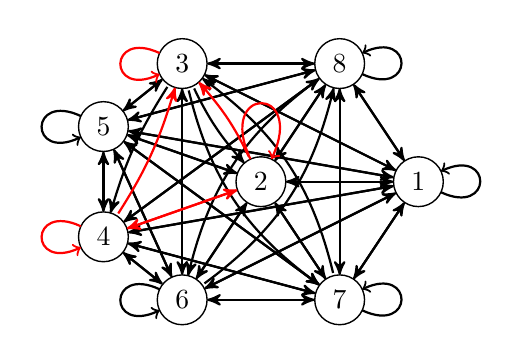
\begin{tikzpicture}[xscale=1,yscale=1]
  \Vertex[L={1},x=2,y=0]{1};
  \Vertex[L={8},x=1,y=1.5]{8};
  \Vertex[L={3},x=-1,y=1.5]{3};
  \Vertex[L={5},x=-2,y=0.7]{5};
  \Vertex[L={4},x=-2,y=-0.7]{4};
  \Vertex[L={6},x=-1,y=-1.5]{6};
  \Vertex[L={7},x=1,y=-1.5]{7};
  \Vertex[L={2},x=0,y=0]{2};
  \SetUpEdge[style={post,{->}, thick}]
  \Edge(1)(2)
  \Edge(1)(3)
  \Edge(1)(4)
  \Edge(1)(5)
  \Edge(1)(6)
  \Edge(1)(7)
  \Edge(1)(8)
  \Edge(2)(1)
  \Edge(2)(5)
  \Edge(2)(6)
  \Edge(2)(7)
  \Edge(2)(8)
  \Edge(3)(1)
  \Edge(3)(5)
  \Edge(3)(6)
  \Edge(3)(8)
  \Edge(4)(1)
  \Edge(4)(5)
  \Edge(4)(6)
  \Edge(4)(7)
  \Edge(4)(8)
  \Edge(5)(1)
  \Edge(5)(2)
  \Edge(5)(3)
  \Edge(5)(4)
  \Edge(5)(6)
  \Edge(5)(7)
  \Edge(5)(8)
  \Edge(6)(1)
  \Edge(6)(2)
  \Edge(6)(3)
  \Edge(6)(4)
  \Edge(6)(5)
  \Edge(6)(7)
  \Edge(7)(1)
  \Edge(7)(2)
  \Edge(7)(4)
  \Edge(7)(5)
  \Edge(7)(6)
  \Edge(7)(8)
  \Edge(8)(1)
  \Edge(8)(2)
  \Edge(8)(3)
  \Edge(8)(4)
  \Edge(8)(5)
  \Edge(8)(7)
  \SetUpEdge[style={post,bend right=20,thick}]
  \Edge(3)(7)
  \Edge(7)(3)
  \Edge(6)(8)
  \Edge(8)(6)
  \SetUpEdge[style={post,thick,color=red}]
  \Edge(2)(4)
  \Edge(4)(2)
  \SetUpEdge[style={post,bend right=8,thick}]
  \Edge(3)(2)
  \Edge(3)(4)
  \SetUpEdge[style={post,bend right=8,thick,color=red}]
  \Edge(2)(3)
  \Edge(4)(3)
  \draw[thick,->] (1) to[out=-25,in=25,looseness=7] (1);
  \draw[thick,->,color=red] (2) to[out=115,in=65,looseness=10] (2);
  \draw[thick,->,color=red] (3) to[out=155,in=205,looseness=7] (3);
  \draw[thick,->,color=red] (4) to[out=155,in=205,looseness=7] (4);
  \draw[thick,->] (5) to[out=155,in=205,looseness=7] (5);
  \draw[thick,->] (6) to[out=155,in=205,looseness=7] (6);
  \draw[thick,->] (7) to[out=-25,in=25,looseness=7] (7);
  \draw[thick,->] (8) to[out=-25,in=25,looseness=7] (8);
  \SetUpEdge[color=red]
\end{tikzpicture}
  \caption{Solution with entropy $\log_2(7.2568898)$.}
  \label{fig:adaptive_cosim_stable}
\end{figure}

We applied \algoref{stabilization} to the lifts of degree 0, 1 and 2. %
At each application of the algorithm, a stable constrained switched system was produced, with an entropy that increased with the degree of the lift.
These results, summarized in \tabref{entropy_over_k}, corroborate \theoref{remove_1_cycle}.

\begin{table}[tbh]
  \centering
  \caption{Entropy achieved per lift degree.}
  \label{tab:entropy_over_k}
  \begin{tabular}{l|l|l}
    $k$ & Entropy [bit] & CPU time [s]\\
    \hline
    0 & $\log_2(5)$ & 0.13\\
    1 & $\log_2(7.2568898)$ & 1.8\\
    2 & $\log_2(7.7083039)$ & 280
  \end{tabular}
\end{table}

This application to co-simulation illustrates an important advantage of the method presented in \secref{certifylowerbound}: it is capable of finding large unstable cycles.
This method does not find the unstable cycles by iterating through the cycles of some length $K$ but instead extracts them from an infinite switching signal,
hence it is not harder for the method to find large unstable cycles.
For the lift of degree 2 for example, it found the unstable cycle $542245332$ of length 9, and in a subsequent iteration found the cycle $224533542245335422453354224523254$ of length 33.
A brute force method would have to enumerate all $8^{33}$ cycles to achieve the stabilization of the adaptive solver.

Regarding the optimality of the solution found for the lift with degree 1, we have applied the procedure detailed in \secref{optimality} to confirm that $\log_2(7.2568898)$ is indeed the maximal entropy for that degree.



\subsection{Conclusion}
\label{sec:conclusion}

As the stability of the system is a set program, we showed in this section how
the rounding algorithm presented in \secref{certifylowerbound}
can be used to restrict the switching possibilities
of a constrained switching systems so as to leave as many
switching policies as possible (provided that the system becomes stable).

Our algorithm takes the form of a hierarchy of sufficient conditions,
where increasingly better solutions are found by lifting the automaton (see \figref{1cycle} and \tabref{entropy_over_k}).
Essentially, this allows one to control the optimality of the solution, at the cost of processing power and memory.




\section{Low rank reduction}
\label{sec:lowrank}

In \cite{ahmadi2012joint}, Ahmadi and Parrilo show how to reduce the computation of the JSR
of matrices that are all of rank one to a combinatorial problem,
which coincides with the CJSR of $1 \times 1$ matrices (i.e. scalars).
As a final contribution, we generalize
this approach and give a reduction of the computation of the JSR (or CJSR)
of matrices that are all of rank at most $r$ to the computation of the CJSR of $r \times r$ matrices.

Suppose we want to compute the CJSR of a finite set of matrices $\A \eqdef \{A_1, \ldots, A_m\} \subset \mathbb{R}^{n \times n}$ of rank at most $r$ constrained by an automaton $\G(V,E)$.
For $\sigma = 1, \ldots, m$, since the matrix $A_\sigma$ has rank at most $r$, there exists $X_\sigma, Y_\sigma \in \mathbb{R}^{n \times r}$ such that $A_\sigma = X_\sigma Y_\sigma^\Tr$.
This can be used to build a new system with matrices of $\R^{r \times r}$ with the same CJSR.
This new system can therefore be used to reduce the computation of the CJSR of a system of low rank matrices to a system of matrices of small size.
Note that in the case $r=1$, it is known that the CJSR is computable in polynomial time~\cite{ahmadi2012joint}.


\begin{mytheo}[Low Rank Reduction]
  \label{theo:lowrank}
  Consider a finite set of matrices $\A \eqdef \{A_1, \ldots, A_m\} \subset \mathbb{R}^{n \times n}$ of rank at most $r$
  constrained by an automaton $\G(V,E)$.

  For a fixed decomposition $A_\sigma = X_\sigma Y_\sigma^T$ for $\sigma = 1, \ldots, m$ where $X_\sigma, Y_\sigma \in \R^{n \times r}$,
  denote the set of matrices $\A' \eqdef \{A_{\sigma_1\sigma_2}' \mid \sigma_1, \sigma_2 = 1, \ldots, m\} \subset \mathbb{R}^{r \times r}$ where $A_{\sigma_1\sigma_2}' = Y_{\sigma_1}^TX_{\sigma_2}$.
  Define the graph $\G'(V',E')$ with $V' \eqdef E$ and
  \[
    E' \eqdef \{\, ((u,v,\sigma_1), (v,w,\sigma_2), \sigma_2\sigma_1) \mid (u,v,\sigma_1),(v,w,\sigma_2) \in E \,\}.
  \]
  Then the two CJSR are the same:
  \( \cjsr = \cjsrp. \)
  \begin{proof}
    As the CJSR does not depend on the norm used, we choose a norm $\|\cdot\|$ that is \emph{submultiplicative},
    that is $\|AB\| \leq \|A\| \|B\|$ for all matrices $A,B$.

    Let $\beta = \max_{\sigma=1}^m\max\{\|X_\sigma\|, \|Y_\sigma^T\|\}$.
    If $\beta = 0$, then $\cjsr = 0 = \cjsrp$.
    Therefore we may assume that $\beta > 0$.
    Consider a positive integer $k$.
    We first show that $[\cjsrk]^k \leq \beta^2[\cjsrkp[k-1]]^{k-1}$
    where $\cjsrk$ is defined in \eqref{eq:cjsrk}.
    For any $\G$-admissible $(\sigma_1, \sigma_2, \ldots, \sigma_k)$, we have
    \begin{equation*}
      \label{eq:redu}
      A_{\sigma_k} \cdots A_{\sigma_2}A_{\sigma_1} = X_{\sigma_k}A_{\sigma_k\sigma_{k-1}}' \cdots A_{\sigma_3\sigma_2}' A_{\sigma_2\sigma_1}'Y_{\sigma_1}^T.
    \end{equation*}
    using
    the submultiplicativity of the norm chosen, we have
    \begin{align*}
      \|A_{\sigma_k} \cdots A_{\sigma_1}\|
      & \leq \|X_{\sigma_k}\| \cdot \|A_{\sigma_k\sigma_{k-1}}' \cdots A_{\sigma_3\sigma_2}' A_{\sigma_2\sigma_1}'\| \cdot \|Y_{\sigma_1}^T\|\\
      & \leq \beta^2\|A_{\sigma_k\sigma_{k-1}}' \cdots A_{\sigma_3\sigma_2}' A_{\sigma_2\sigma_1}'\|\\
      & \leq \beta^2 [\cjsrkp[k-1]]^{k-1}.
    \end{align*}

    The same way, we now show that $[\cjsrkp[k-1]]^{k-1} \leq \beta^2 [\cjsrk[k-2]]^{k-2}$.
    For any $\G'$-admissible $(\sigma_2\sigma_1, \ldots, \sigma_k\sigma_{k-1})$, we have
    \begin{align*}
      \|A_{\sigma_k\sigma_{k-1}}' \cdots A_{\sigma_3\sigma_2}' A_{\sigma_2\sigma_1}'\|
      & \leq \|Y_k^T\| \cdot \|A_{\sigma_{k-1}} \cdots A_{\sigma_2}\| \cdot \|X_1\|\\
      & \leq \beta^2 [\cjsrk[k-2]]^{k-2}.
    \end{align*}

    In summary, we have
    \begin{align*}
      \cjsrk
      & \leq \beta^{\frac{2}{k}} [\cjsrkp[k-1]]^{\frac{k-1}{k}}\\
      & \leq \beta^{\frac{4}{k}} [\cjsrk[k-2]]^{\frac{k-2}{k}}.
    \end{align*}
    Taking the limit $k \to \infty$ we get $\cjsr \leq \cjsrp \leq \cjsr$.
  \end{proof}
\end{mytheo}

\begin{myexem}
  Consider an unconstrained switched system with 2 rank $r$ matrices $A_1, A_2$.
  This system is equivalent to the constrained switched system with automaton represented in \figref{redu1}.
  Its low rank reduction is represented in \figref{redu2}.
  \begin{figure}[!ht]
    \begin{subfigure}{0.49\textwidth}
      \centering
      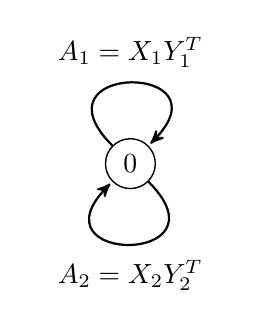
\begin{tikzpicture}
        \SetGraphUnit{3}
        \GraphInit[vstyle=Dijkstra]
        \SetUpEdge[style={->}]
        \Vertex{0}
        \Loop[labelstyle={above=2pt,fill=white},dist=1.5cm,dir=NO,label={$A_1 = X_1Y_1^T$}](0)
        \Loop[labelstyle={below=2pt,fill=white},dist=1.5cm,dir=SO,label={$A_2 = X_2Y_2^T$}](0)
      \end{tikzpicture}
      \caption{Automaton $\G$.
      We
      have $V = \{0\}$ and $E = \{(0,0,1),(0,0,2)\}$.}
      \label{fig:redu1}
    \end{subfigure}~%
    \hfill%
    \begin{subfigure}{0.49\textwidth}
      \centering
      \begin{tikzpicture}
        \SetGraphUnit{3}
        \SetUpEdge[style={->}]%
        \tikzset{EdgeStyle/.style = {distance = 30}}
        \Vertex[NoLabel=false]{1}
        \EA[NoLabel=false](1){2}
        \tikzset{EdgeStyle/.append style = {bend right=60}}
        \Loop[labelstyle={above=0pt},dist=1.5cm,dir=EA,label={$A_{11}' = Y_1^TX_1$}](1)
        \Loop[labelstyle={above=0pt},dist=1.5cm,dir=EA,label={$A_{22}' = Y_2^TX_2$}](2)
        \Edge[labelstyle={above=4pt, fill opacity=0, text opacity=1},label={$A_{21}' = Y_2^\Tr X_1$}](1)(2)
        \Edge[labelstyle={below=4pt, fill opacity=0, text opacity=1},label={$A_{12}' = Y_1^\Tr X_2$}](2)(1)
      \end{tikzpicture}
      \caption{Automaton $\G'$.
      We have $V' \allowbreak= \allowbreak\{1,2\}$ and
      $E' = \{(1,1,11),\allowbreak (1,2,21),\allowbreak (2,1,12),\allowbreak (2,2,22)\}$.}
      \label{fig:redu2}
    \end{subfigure}
    \caption{Simple example of the low rank reduction.}
    \label{fig:redu}
  \end{figure}
\end{myexem}

\begin{myrem}
  The matrices $X_\sigma, Y_\sigma$ of the factorization $A_\sigma = X_\sigma Y_\sigma^T$ are not unique.
  For any invertible matrix $S \in \mathbb{R}^{r \times r}$, $A_\sigma = (X_\sigma S)(S^{-1}Y_\sigma^T)$ also gives a factorization.
  However, if $\cjsrp$ is approximated using \progref{primal},
  any two factorizations will give the same approximation.
  The effect of using $X_\sigma S$ and $Y_\sigma S^{-T}$ instead of $X_\sigma$ and $Y_\sigma$ will simply be a linear change of variable of the polynomial $p_\sigma$. %

\end{myrem}

What is the impact of this reduction on the computational complexity and accuracy of the approximation ?
The entropy of the language of allowed switching signals is the same for the initial system and the reduced system hence the guarantee in \theoref{second} is the same for both systems.
However, the dimension of the matrices goes from the dimension of the matrices $n$ to their rank $r$
hence for low rank matrices the guarantee in \theoref{matt} is improved.

In terms of computational complexity, there can be up to $m$ \nodes{} and $m^2$ \arcs{} in the automaton of the reduced system.
Therefore, even if the size of the matrices decreases from $n$ to $r$, the number of variables and constraints increases.
This shows that the reduction only decreases the computational complexity if the rank of the matrices is \emph{sufficiently} low.





\section{Conclusion}

We have analyzed in details the set program with
constraints of the form~\eqref{eq:imageincl} or \eqref{eq:preimageincl}
for polysets of degree $2d$.
We showed that one guarantee is tight in \secref{unconstrguarantee} and
provided a new guarantee in \secref{entropyguarantee} but
in practice, the performance exceeds the worst-case expectation based on these guarantees.
One promising direction might be to provide a guarantee based on the matrices describing the switched system,
similarly to the guarantee of \conjref{jcn} based on the joint condition number of the input matrices of the set program.

In \secref{certifylowerbound}, we showed how to exploit the
infeasibility certificate of a set program for polysets in order to certify the
infeasibility of the generic set program and in \secref{switchstab},
we showed how to minimally relax the set program in order to render it feasible.
It is however unclear why this approach would be specific to the class of set
programs studied in this section and it would be compelling to extend this
technique to other classes of set programs.

\chapter{Stabilizability}
\label{chap:mci}

As mentioned in the introduction of \secref{control},
the computation of controlled invariant set is a key problem in System and Control theory.
The design of an efficient algorithm for computing controlled invariant sets
of a class of systems renders many important problems efficiently solvable; see \cite{blanchini1999survey} for more details.
We introduced in \secref{control} an algebraic approach for the computation of
controlled invariant ellipsoids using the LMI~\eqref{eq:disc_control_LMI}.

An alternative approach to \eqref{eq:disc_control_LMI} for computing ellipsoidal
controlled invariant sets was introduced in \cite{legat2018computing, legat2020sum, legat2020piecewiseCO}. A key
ingredient in this technique is that the problem is formulated in the dual space
of the geometric problem. It leverages duality like
\cite{boyd1994linear, ahmadi2015robust} but contrary to them it combines it with
a projection of the state space to its subspace that is not \emph{directly} %
controllable.
Compared to the method described above, with this approach the \emph{controlled}
invariance LMI constraint has size $n \times n$ and not $(2n) \times (2n)$.
Both methods solve the problem in the dual space as the ellipsoid
$\mathcal{E}_{P^{-1}}$ is the polar of the ellipsoid $\mathcal{E}_{P}$.
However, the method of \cite{legat2018computing, legat2020sum, legat2020piecewiseCO} is developed at the abstract level of sets
instead of relying on algebraic manipulation at the level of matrices.
As shown in \chapref{setprog},
this allows the method to be extended to other templates
such as piecewise semi-ellipsoids, polysets and piecewise polysets.

In \secref{mci_continuous}, we show how to use this geometric approach
to compute controlled invariant set for a continuout-time control systems~\eqref{eq:contcontrolsys}.

In \secref{mci_discrete}, we show how to use the results
of \secref{preimage} to compute controlled invariant sets for discrete-time control systems.
We detail the application of the method to two classes of hybrid systems:
Discrete-Time Affine Hybrid Control System (\dtahcs{} for short) and Discrete-Time Affine Hybrid Algebraic System (\dtahas{} for short).
\dtahas{} are not control systems but the computation of invariant sets for such systems presents
the same features than for \dtahcs{}.


As the computation of controlled invariant sets of a \dtahcs{} has been reduced
to the computation of invariant sets of a \dtahas{}, we describe in
\secref{mci_discrete} our method to compute invariant sets of \dtahas{} as ellipsoids
or polysets.
In \secref{hellipsoids}, we show that using the results of \secref{preimage}, the
invariance of ellipsoids for a \emph{homogeneous} \dtahas{}, see \defref{homogeneous},
can be formulated as a semidefinite program.
In \secref{ellipsoids}, we show how to use homogenization technique developed in \secref{homogenization} to
generalize the semidefinite program of \secref{hellipsoids} to non-homogeneous
\dtahas{}.
In \secref{controlsos}, we generalize the semidefinite program of \secref{hellipsoids}
to compute invariant polysets of arbitrary degree.

We end the chapter with an application of the controlled invariant sets to safety
critical model predictive control in \secref{mpc} and stochastic programming in \secref{stochprog}.
We show that precomputing such sets allows to guarantee safety of the model
predictive controller %
thereby removing the need for long horizon in model predictive control
and infeasibility cuts in stochastic programming.


\section{Continuous-time}
\label{sec:mci_continuous}

\begin{myprop}
  \label{prop:csas}
  A set $S$ is controlled invariant for control system~\eqref{eq:contcontrolsys} with $\mathcal{U} = \R^{n_u}$ if and only if
  it is controlled invariant for the control algebraic system~\eqref{eq:contcontrolalgsys}
  \[ \piB{}\dot{x} = \piB{}Ax \]
  where $\piB{}$ is an orthogonal projection matrix with range $\Image(B)^\perp$, the orthogonal complement of the linear subspace $\Image(B)$.
  \begin{proof}
    By \propref{projB}, there exists $u \in \R^{n_u}$ such that $\dot{x} = Ax + Bu$
    if and only if $\piB{}\dot{x} = \piB{}Ax$.
    As the input $u$ is unconstrained, the result follows.
  \end{proof}
\end{myprop}

\begin{myprop}[{Nagumo condition~\cite[Theorem~4.7]{blanchini2015set}}]
  \label{prop:nagumo}
  A closed set $S$ is invariant for system \eqref{eq:contcontrolalgsys} if and only if
  \begin{equation}
    \label{eq:invtang}
    \forall x \in \partial S, \exists y \in T_S(x), Ey = Ax.
  \end{equation}
\end{myprop}

The Nagumo condition can then be expressed in terms of the normal cone instead of the tangent cone,
as we will see in \eqref{eq:invnorm}.


\begin{mytheo}[Controlled invariance of convex set]
  \label{theo:invconvex}
  A convex set $\Csetvar$ is invariant for system \eqref{eq:contcontrolalgsys}
  with matrices $A, E \in \mathbb{R}^{r \times n}$
  if and only if
  \begin{equation}
    \label{eq:invface}
    \forall z \in \mathbb{R}^r, \forall x \in F_\Csetvar(E^\Tr z), \la z, Ax \ra \le 0.
  \end{equation}
  \begin{proof}
    As $\Csetvar$ is convex, $T_S(x)$ is a convex cone. By definition
    of the polar of a cone, $x \in ET_S(x)$ if and only if
    $\langle y, x \rangle \le 0$ for all $y \in \polar{[ET_S(x)]}$.
    By \propref{podu}, $\polar{[ET_S(x)]} = E^{-\Tr}N_S(x)$.
    Therefore, the set $\Csetvar$ is invariant if and only if
    \begin{equation}
      \label{eq:invnorm}
      \forall x \in \partial \Csetvar, \forall z \in E^{-\Tr} N_\Csetvar(x), \langle z, Ax \rangle \le 0.
    \end{equation}
    By \propref{normalsupfun}, we have
    \begin{multline*}
      \{\, (x, z) \in \partial \Csetvar \times \mathbb{R}^r \mid E^\Tr z \in N_\Csetvar(x) \,\} = %
      \{\, (x, z) \in \partial \Csetvar \times \mathbb{R}^r \mid x \in F_\Csetvar(E^\Tr z) \,\}.
    \end{multline*}
    As $\Image(F_\Csetvar) \subseteq \partial \Csetvar$ (with equality if every face is exposed),
    we obtain \eqref{eq:invface}.
  \end{proof}
\end{mytheo}

\begin{mytheo}
  \label{theo:invexposed}
  Consider a nonempty closed convex set $\Csetvar$ such that
  $\supfun{\cdot}{\Csetvar}$ is differentiable.
  Then $\Csetvar$ is invariant for system \eqref{eq:contcontrolalgsys}
  with matrices $A, E \in \mathbb{R}^{r \times n}$
  if and only if
  \begin{equation}
    \label{eq:invgrad}
    \forall z \in \mathbb{R}^r, \la z, A \grad \supfun{E^\Tr z}{\Csetvar} \ra \le 0.
  \end{equation}
  \begin{proof}
    By \propref{exposed}, $F_\Csetvar(E^\Tr z) = \{\grad \supfun{E^\Tr z}{\Csetvar}\}$
    hence \eqref{eq:invface} is equivalent to \eqref{eq:invgrad}.
  \end{proof}
\end{mytheo}

\subsection{Ellipsoid template}
Note that while the quadratically stabilizable systems of the form \eqref{eq:contcontrolsys}
is equivalent to their quadratically stabilizable via linear control, it is no longer
the case for \emph{uncertain} or \emph{switched} systems.


Since the support function of an ellipsoid $\mathcal{E}_P$ is $\supfun{y}{\mathcal{E}_P} = \sqrt{y^\Tr P y}$,
we have the following corollary of \theoref{invexposed}.
\begin{mycoro}
  Given a positive definite matrix $P$, the ellipsoid $\mathcal{E}_P$ is
  controlled invariant for system~\eqref{eq:contcontrolalgsys} if and only if
  \begin{equation}
    \label{eq:invLMI}
    AP^{-1}E^\Tr + EP^{-1}A^\Tr \preceq 0.
  \end{equation}
\end{mycoro}

Note that for the trivial case $\Image(B) = \mathbb{R}^n$ for system~\eqref{eq:contcontrolsys},
the \propref{csas}, will produce a system~\eqref{eq:contcontrolalgsys} with $r = 0$ hence the
LMI~\eqref{eq:invLMI} will be trivially satisfied for any $P^{-1}$ which is expected.

In comparison to \eqref{eq:cont_control_LMI}, for a system~\eqref{eq:contcontrolalgsys} with matrices
$A, E \in \mathbb{R}^{r \times n}$, the LMI~\eqref{eq:cont_control_LMI} has
size $n \times n$ while the LMI~\eqref{eq:invLMI} has only size $r \times r$.
The characterization of controlled invariance of ellipsoids using \eqref{eq:invLMI}
can also be obtained by applying an elimination procedure to reduce \eqref{eq:cont_control_LMI};
see \cite[Equation~(7.11)]{boyd1994linear}.
However, uncertain or switched system may need a nonlinear state feedback to be quadratically
stabilizabilized~\cite{petersen1985quadratic}.
For such systems, \eqref{eq:cont_control_LMI} is conservative since it assumes a linear feedback
while \eqref{eq:invLMI} does not assume anything about the feedback.
It was shown in \cite{barmish1985necessary} that if \eqref{eq:invLMI} is satisfied then a stabilizing nonlinear continous
state feedback can be deduced from the solution $P$.
There is even a closed form for the feedback in case of single input~\cite[Eq.~(15)]{barmish1985necessary}.

\subsection{Polyset template}
Moreover, to find invariant sets more sophisticated than ellipsoids, we can simply
search for sets such that the support function is a polynomial.
\begin{mycoro}
  Given an homogeneous nonnegative polynomial $p(x)$ of degree $2d$, the set $\Csetvar$ of support function
  $\supfun{y}{\Csetvar} = p(y)^{\frac{1}{2d}}$
  is invariant for system~\eqref{eq:contcontrolalgsys}
  with matrices $A, E \in \mathbb{R}^{r \times n}$
  if and only if the polynomial
  \begin{equation}
    \label{eq:invSOS}
    z^\Tr A \grad p(E^\Tr z)
  \end{equation}
  is nonpositive for all $z \in \mathbb{R}^r$.
  \begin{proof}
    We have
    \[
      \grad \supfun{y}{\Csetvar} = \frac{1}{p(y)^{1-\frac{1}{2d}}} \grad p(y)
    \]
    and since $p(y)^{1-\frac{1}{2d}}$ is positive,
    \eqref{eq:invgrad} is equivalent to \eqref{eq:invSOS}.
  \end{proof}
\end{mycoro}
While verifying the nonnegativity of polynomials is co-NP-hard,
we can find invariant sets by restricting them to be SOS as described in \secref{sosprog}.


\section{Discrete-time}
\label{sec:mci_discrete}



\subsection{Ellipsoid template for homogeneous systems}
\label{sec:hellipsoids}
In this section, we show how to compute ellipsoidal controlled invariant sets using \theoref{controlineq} and \eqref{eq:ellalgincl} in the particular case of homogeneous \dtahcs{} and \dtahas{}.
We show how to handle non-homogeneity in \secref{ellipsoids} and how to use more general sets in \secref{controlsos};
we start by describing the ellipsoidal homogeneous case for clarity.
This section details the semidefinite program needed to find these ellipsoidal invariant sets and shows its exactness in \theoref{hquad}.

The optimization problem to solve is given in \progref{hquad}.
The complexity for solving the semidefinite program is given by \eqref{eq:sdp_complexity}
where $n$ and $m$ depends on whether the program is written in the standard form \eqref{eq:sdp_standard} or the conic form \eqref{eq:sdp_conic} but in either cases, it depends affinely on the state dimension, the number of \nodes{} and the number of transitions of the system.
We use the notation $p_q(x, z)$ to denote the evaluation of $p_q$ at the vector $y = (x, z)$.

\begin{myprog}
  \label{prog:hquad}
  \begin{align}
    \notag
    \max_{D_q \succ 0}
    & \quad \sum_{q \in \Nodes} \log \det D_q\\
      \label{eq:hquads}
      A_\sigma D_q A_\sigma^\Tr & \preceq E_\sigma D_{q'} E_\sigma^\Tr,
      && \forall q \trs q'\\
      \label{eq:hquadc}
      a^\Tr D_q a & \leq \beta^2,
      && \forall q \in \Nodes, (a, \beta) \in \Hrep(\Ps_q)
  \end{align}
  where $\Hrep(\Ps_Q)$ denotes the set of all $(a, \beta)$ such that the half-space $a^\Tr x \leq \beta$ supports $\Ps_q$,
  which is commonly referred to as its H-representation~\cite{ziegler1995lectures}.
\end{myprog}

The constraint \eqref{eq:hquads} is \eqref{eq:ellalgincl}, it ensures invariance of the set.
The constraint \eqref{eq:hquadc} ensures that $\Csetvar_q$ is contained in $\Ps_q$.

\begin{myrem}
  \label{rem:obj}
  As we show in \theoref{hquad}, \eqref{eq:hquads} and \eqref{eq:hquadc} ensures
  that only invariant ellipsoids are feasible for \progref{hquad}.
  The most \emph{relevant} solution among all feasible solutions depends on the application.
  Hence the objective function may involve some or all the ellipsoids and use
  one metric or another depending on the purpose of the optimization.
  We consider the sum of the $\log \det D_q$ in \progref{hquad} but it can be
  replaced by any of the variations listed in \secref{ellvol}.
\end{myrem}


\begin{mytheo}
  \label{theo:hquad}
  Consider a homogeneous \dtahas{} $\sys$ as in \defref{dtahas}.
  The symmetric matrix $D_q$ is feasible for \progref{hquad} if and only if
  there exist invariant convex sets $\Csetvar = (\Csetvar_q)_{q \in \Nodes}$,
  as defined in \defref{is},
  such that $\Csetvar_q^\circ = \Ell{D_q}$ for all $q \in \Nodes{}$.
  Moreover, the optimal solution of \progref{hquad} is the solution that maximizes
  the sum of the logarithms of the volume of the ellipsoids.
  \begin{proof}
    We first show that \eqref{eq:hquads} is equivalent to the invariance of the sets $\Csetvar_q$.
    By \theoref{controlineq} and \eqref{eq:ellalgincl}, the invariance of the sets $\Csetvar_q$ is equivalent to \eqref{eq:hquads}.

    We now show that \eqref{eq:hquadc} is equivalent to $\Csetvar_q \subseteq \Ps_q$.
    Since $\Ps_q$ is symmetric,
    it is the intersection of pairs of half-spaces $-\beta \leq \la a, x \ra \leq \beta$ and
    $\Csetvar_q \subseteq \Ps_q$ if and only if $a/\beta, -a/\beta \in \polar{\Csetvar_q}$ for each pair of half-spaces.
    Since $\polar{\Csetvar_q} = \Ell{D_q}$, this is equivalent to \eqref{eq:hquadc}.
  \end{proof}
\end{mytheo}

\subsection{Ellipsoid template for non-homogeneous systems}
\label{sec:ellipsoids}
In this section, we show how to adapt \progref{hquad} in the case of non-homogeneous systems using the homogenization technique detailed in \secref{homogenization}.
The non-homogeneous version of \theoref{controlineq} is given as follows.

\begin{mytheo}
  \label{theo:dtahas}
  Consider a \dtahas{} $\sys$ as in \defref{dtahas}. %
  The closed convex sets $\Csetvar = (\Csetvar_q)_{q \in \Nodes}$ are \emph{invariant} for $\sys$,
  as defined in \defref{is}, if and only if
  $\Csetvar_q \subseteq \Ps_q$ for each $q \in \Nodes$ and
  for all $q \trs q'$,
  \begin{equation}
    \label{eq:dtahas}
    r(A_\sigma, c_\sigma)^{-\Tr} \tau(\Csetvar_q)^* \supseteq r(E_\sigma, 0)^{-\Tr} \tau(\Csetvar_{q'})^*.
  \end{equation}
  \begin{proof}
    The invariance constraint~\eqref{eq:isdtahas} of \defref{is}
    \[ A_\sigma \Csetvar_q + c_\sigma \subseteq E_\sigma \Csetvar_{q'} \]
    can be rewritten, using \eqref{eq:taur}, into
    \begin{equation}
      \label{eq:coneinv}
      r(A_\sigma, c_\sigma) \tau(\Csetvar_q) \subseteq r(E_\sigma, 0) \tau(\Csetvar_{q'}).
    \end{equation}
    As the sets $\Csetvar_q$ are closed and convex, so are the cones $\tau(\Csetvar_q)$
    hence $\tau(\Csetvar_q)^{**} = \tau(\Csetvar_q)$.
    Therefore, by \propref{podu}, \eqref{eq:coneinv} is equivalent to \eqref{eq:dtahas}.
  \end{proof}
\end{mytheo}


The optimization problem to solve is represented in \progref{quad}.
To transform this program into a semidefinite program,
the equality~\eqref{eq:quadp} between quadratic forms is replaced by an equality corresponding
to the coefficient of each quadratic monomial in $y$ and
the inequality~\eqref{eq:quads} between quadratic forms is replaced by an LMI constraint.
The complexity for solving the semidefinite program is given by \eqref{eq:sdp_complexity}
where $n$ and $m$ depends on whether the program is written in the standard form \eqref{eq:sdp_standard} or the conic form \eqref{eq:sdp_conic} but in either cases, it depends affinely on the state dimension, the number of \nodes{} and the number of transitions of the system.
We use the notation $p_q(x, z)$ to denote the evaluation of $p_q$ at the vector $y = (x, z)$.

\begin{myprog}
  \label{prog:quad}
  \begin{align}
    \notag
    \max_{\substack{D_q \in \SymK, d_q \in \R^n,\\\delta_q \in \R, \lambda_{q \trs q'} \geq 0}}
    & \quad \sum_{q \in \Nodes} \log \det D_q
    \\
    \label{eq:quadl1}
    \begin{bmatrix}
      D_q & d_q\\
      d_q^\Tr & \delta_q + 1
    \end{bmatrix} & \succ 0\\ %
    \label{eq:quadp}
    p_q(y) & = y^\Tr \House{h_q}
    \begin{bmatrix}
      D_q & d_q\\
      d_q^\Tr & \delta_q
    \end{bmatrix}
    \House{h_q} y\\
    \label{eq:quads}
    p_q(r(A_\sigma, c_\sigma)^\Tr y) & \leq \lambda_{q \trs q'} p_{q'}(r(E_\sigma, 0)^{\Tr} y),
    && \forall q \trs q', y \in \R^{\nqx+1}\\
    \label{eq:quadc}
    p_q(-a, \beta) & \leq 0,
    && \forall q \in \Nodes, (a, \beta) \in \Hrep(\Ps_q)\\
    \label{eq:quadf}
    p_q(0, 1) & < 0,
    && \forall q \in \Nodes.
  \end{align}
\end{myprog}

The constraint \eqref{eq:quadl1} ensures both convexity of $\tau(\Csetvar_q)^*$ and the fact that $\det D_q$ does not overestimate the volume of the ellipsoid transformed by the Householder reflection.
The constraint \eqref{eq:quads} is the S-procedure applied to the condition \eqref{eq:dtahas}.
The constraint \eqref{eq:quadc} uses \eqref{eq:hs} to ensure that $\Csetvar_q$ is contained in $\Ps_q$.
The constraint \eqref{eq:quadf} ensures that $\tau(\Csetvar_q)^*$ has non-empty interior.
Note that if $\Ps_q$ has no unbounded subspace, \eqref{eq:quadf} is not necessary since the non-empty interior condition will already be ensured by \eqref{eq:quadc}.

\begin{mytheo}
  \label{theo:quad}
  Consider a \dtahas{} $\sys$ as in \defref{dtahas} and points $(h_q \in \Ps_q)_{q \in \Nodes}$.
  The polynomial $p_q(x, z)$ is feasible for \progref{quad} if and only if
  there exist invariant convex sets $\Csetvar = (\Csetvar_q)_{q \in \Nodes}$,
  as defined in \defref{is},
  such that $h_q \in \Csetvar_q$ for each $q \in \Nodes$
  and $\tau(\Csetvar_q)^*$ is the 0-sublevel set of $p_q(x, z)$.
  Moreover, the optimal solution of \progref{quad} is the solution that minimizes
  the sum of the logarithms of the volume of the intersection of the each cone $\tau(\Csetvar_q)^*$ with the hyperplane
  \( \{\, x \mid \langle h_q, x \rangle = 1 \,\}. \)
  \begin{proof}
    Consider a solution $p = (p_q(x, z))_{q \in \Nodes}$ of \progref{quad}.
    By \cororef{convexcone}, constraints \eqref{eq:quadl1} and \eqref{eq:quadp} are satisfied if and only if there exist ellipsoids $\Csetvar_q$ such that $\tau(\Csetvar_q)^*$ is the 0-sublevel set of $p_q(x, z)$.
    By \eqref{eq:hs}, constraint \eqref{eq:quadc} is satisfied if and only if $\Csetvar_q \subseteq \Ps_q$.
    By \propref{sproc}, constraint \eqref{eq:quads} is satisfied if and only if
    \eqref{eq:dtahas} hold for all $q \trs q'$.
    Therefore, by \theoref{dtahas}, the solution $p$ is a feasible solution of \progref{quad} if and only if the sets $\Csetvar_q$ are invariant for $\sys$.

    We now prove the optimality of the solution.
    By \propref{QD}, there exist $Q_q, c_q$ such that $\Ellc{Q_q}{c_q} = \Ellq{D_q}{d_q}{\delta_q}$ and $\lambda_q > 0$ such that $D_q = \lambda_q Q_q$.
    The volume of the intersection of $\tau(\Csetvar_q)^*$ with the hyperplane
    \( \{\, x \mid \langle h_q, x \rangle = 1 \,\} \)
    is $-\det(Q_q)$.
    Therefore, it remains to show that $\lambda_q = 1$ for an optimal solution.
    We observe that without the constraint~\eqref{eq:quadl1}, for any feasible solution, $D_q, d_q, \delta_q$ can be scaled by any positive constant
    while remaining feasible but affecting the objective function.
    The Schur complement (see \propref{schurcomp}) of the block $D_q$ of the matrix in the
    left-hand side of constraint~\eqref{eq:quadl1} is
    $\delta_q + 1 - d_q^\Tr D_q^{-1} d_q$ hence constraint~\eqref{eq:quadl1}
    ensures that
    \[ d_q^\Tr D_q^{-1} d_q - \delta_q \leq 1. \]
    Combining this inequality with equation~\eqref{eq:lambda} implies that $\lambda_q \leq 1$.
    Since the objective is to maximize $\det(D_q) = \lambda_q \det(Q_q)$,
    we know that if $(D_q, d_q, \delta_q)$ is optimal,
    then $\lambda_q = d_q^\Tr D_q^{-1} d_q - \delta_q = 1$.
  \end{proof}
\end{mytheo}

\begin{myexem}
  \label{exem:cruise3}
  We apply \progref{quad} to \exemref{cruise2} with the same values for the parameters as the ones used in \cite{rungger2013specification},
  that is, $m_0 = \SI{500}{\kilogram}$, $m = \SI{1000}{\kilogram}$, $k_d = \SI{4600}{\newton\second\per\meter}$ and $k_s = \SI{4500}{\newton\per\kilogram}$.
  The values used for $h_q$ are the same for each \node{} $q \in \Nodes$: $u = d_i = 0$ and $v_0 = v_i = (5+v_a)/2$ for $i = 1, \ldots, M$. %

  We vary the number of trailers $M$ from 1 to 10.
  \figref{cruisesets} represents the controlled invariant set at \node{} $q_{a0}$.
  As we can see, the constraints on the trailers are propagated to the truck and, as the number $M$ increases, the truck speed and acceleration become more constrained.

  The time taken by MOSEK 8.1.0.34 (\cite{mosek2017mosek81034}) to solve the problem is given by \figref{cruisebench}\footnote{We set $\lambda_{q \trs q'}$ to 1 for each transition $q \trs q'$ to make the problem convex.}.
\end{myexem}

\begin{figure}[!h]
  \centering
  \includegraphics[width=0.48\textwidth]{CruiseControlSets_d_v1.png}
  ~
  \includegraphics[width=0.48\textwidth]{CruiseControlSets_v0_u.png}

  \includegraphics[width=0.48\textwidth]{CruiseControlSets_d_u.png}
  ~
  \includegraphics[width=0.48\textwidth]{CruiseControlSets_v1_v0.png}

  \includegraphics[width=0.48\textwidth]{CruiseControlSets_d_v0.png}
  ~
  \includegraphics[width=0.48\textwidth]{CruiseControlSets_v1_u.png}
  \caption{Several projections of the optimal solution of \progref{quad} (in green)
  and \progref{sos} with the volume heuristic developed in \cite{dabbene2017simple} (in orange for quartic, red for sextic and blue for octic)
  for \exemref{cruise3} at \node{} $q_{a0}$ for various numbers of trailers.}
  \label{fig:cruisesets}
\end{figure}

\begin{figure}[!h]
  \centering
  \includegraphics[width=0.8\textwidth]{CruiseControlBenchmark.png}
  \caption{Computation time with MOSEK 8.1.0.34 for \progref{quad} with \exemref{cruise3} with various numbers of trailers compared
  to two iterations of the polyhedral approach (see e.g., the procedure p.~201 in \cite{blanchini2015set}) implemented with the CDD library \cite{fukuda1999cdd}.
  Note that after two iterations, the polyhedral sets obtained are not controlled invariant.
  One needs to wait for the convergence of the algorithm to obtain a controlled invariant set.
  Moreover, iterations are usually increasingly slower as the number of facets of the polyhedral sets increases with the iterations.
  }
  \label{fig:cruisebench}
\end{figure}

\subsection{Polyset template for non-homogeneous systems}
\label{sec:controlsos}

In this section, we generalize the results of Section~\ref{sec:ellipsoids} to polysets.
Note that the last variable of the polynomial is the \emph{perspective} variable of the cone defined in \eqref{eq:tau}.
Therefore, it is not conservative to consider homogeneous polynomials as cones cannot be the sublevel set of non-homogeneous polynomials.

The main challenge of this generalization resides in constraint \eqref{eq:quadl1} ensuring both convexity of $\tau(\Csetvar_q)^*$ and the fact that $\det D_q$ does not overestimate the volume.
Indeed, while checking the convexity and computing the volume of ellipsoids can be done easily,
it is more involved when using polynomials of higher degree as described in \secref{sosconv}.
The volume objective for polyset is discussed in \secref{polysetvol}.

The following program searches invariant polysets of degree $2d$ parametrized by homogeneous polynomials $p_q(x)$.
For increasing degree $d$, the approximation capability of the polysets is improved
at the expense of increased computational time; see \secref{sosprog} for a discussion on the computational complexity of Sum-of-Squares programs.
We use the notation $p_q(x, z)$ to denote the evaluation of $p_q$ at the vector $y = (x, z)$.

\begin{myprog}
  \label{prog:sos}
  \begin{align}
    \label{eq:sos}
    s_q(x, z) + z^{2d} & \text{ is SOS}\\
    \label{eq:sosconvex}
    s_q(x, 1) & \text{ is SOS-convex}\\
    \label{eq:sos_house}
    s_q(x, z) & = p_q(\House{h_q} (x, z)),
    && \forall x \in \R^{\nqx}, z \in \R\\
    \label{eq:soss}
    p_q(r(A_\sigma, c_\sigma)^\Tr y) & \leq \lambda_{q \trs q'} p_{q'}(r(E_\sigma, 0)^{\Tr} y),
    && \forall q \trs q', y \in \R^{\nqx+1}\\
    \label{eq:sosc}
    p_q(-a, \beta) & \leq 0,
    && \forall q \in \Nodes, (a, \beta) \in \Hrep(\Ps_q)\\
    \label{eq:sosf}
    p_q(0, 1) & < 0,
    && \forall q \in \Nodes.
  \end{align}
\end{myprog}

The constraint \eqref{eq:sosconvex} ensure the convexity of $\tau(\Csetvar_q)^*$
and constraints \eqref{eq:soss}, \eqref{eq:sosc} and \eqref{eq:sosf} are identical to the corresponding constraints of \progref{quad}.
The constraint \eqref{eq:sos} is the generalization of \eqref{eq:quadl1} for polynomials
of arbitrary degree.
It certifies that $s_q(x, 1) + 1$ is nonnegative which is required
for heuristics such as \cite{magnani2005tractable, dabbene2017simple} to estimate
the volume of its 1-sublevel set.



\begin{mytheo}
  \label{theo:controlsos}
  Consider a \dtahas{} $\sys$ as in \defref{dtahas} and points $(h_q \in \Ps_q)_{q \in \Nodes}$.
  The polynomial $p_q(x, z)$ is feasible for \progref{sos} if and only if
  there exist invariant convex sets $\Csetvar = (\Csetvar_q)_{q \in \Nodes}$,
  as defined in \defref{is},
  such that $h_q \in \Csetvar_q$ for each $q \in \Nodes$
  and $\tau(\Csetvar_q)^*$ is the 0-sublevel set of $p_q(x, z)$.
  \begin{proof}
    Consider a solution $p = (p_q(x, z), s_q(x, z))_{q \in \Nodes}$ of \progref{sos}.
    By \eqref{eq:sosconvex}, the 0-sublevel set of $s_q(x, z)$ is convex.
    As the 0-sublevel set of $p_q(x, z)$ is its image under the Householder
    transformation, it is also convex.
    Therefore there exist sets $\Csetvar_q$ such that $\tau(\Csetvar_q)^*$ is
    the 0-sublevel set of $p_q(x, z)$.
    By \eqref{eq:hs}, constraint \eqref{eq:quadc} is satisfied if and only if $\Csetvar_q \subseteq \Ps_q$.
    By \propref{sproc}, constraint \eqref{eq:quads} is satisfied if and only if
    \eqref{eq:dtahas} hold for all $q \trs q'$.
    Therefore, by \theoref{dtahas}, the solution $p$ is a feasible solution of \progref{quad} if and only if the sets $\Csetvar_q$ are invariant for $\sys$.
  \end{proof}
\end{mytheo}



\section{Model Predictive Control}
\label{sec:mpc}

As mentioned in the introduction, the controlled invariant sets can be used to derive a feedback control law.
We illustrate this with a Model Predictive Control (MPC) numerical experiment.
We consider a truck with one trailer ($M = 1$) as in \exemref{cruise3}.
The truck starts with speeds $v_0 = v_1 = \SI{2}{\meter\per\second}$ and spring elongation $d = \SI{0}{\meter}$
and has as objective to maximize the distance covered in \SI{20}{\second}.
The maximal speed is initially \SI{4}{\meter\per\second} but after \SI{10}{\second}, it drops to $v_a = \SI{3}{\meter\per\second}$.

In a classical MPC controller, the truck acceleration $u$ is controlled by solving a constrained optimal control problem up to horizon $H$.
We observe that if $H \leq \SI{2.5}{\second}$, the controller is at some point unable to find values of $u$ satisfying input constraints %
such that the state remains in the safe set.

For safety-critical applications, this lack of guarantee is not acceptable as it is necessary to be certain that the system can remain in the safe set.
Moreover, in a real-time context, the need to pick a large horizon is problematic as it increases the cost of online computations.
In our setting, we constrain the state to remain in the controlled invariant sets computed in \exemref{cruise3}\footnote{
  \exemref{cruise3} corresponds to an MPC controller of horizon \SI{0.8}{\second}.
  An MPC controller of different horizons computes different controlled invariant sets by updating the hybrid system accordingly.
} and thereby solve both issues;
safety is guaranteed for arbitrarily long simulations and the length of the horizon does not influence safety so smaller length can be used.
Note that the controlled invariant sets can be computed offline so if it allows to reduce the horizon length,
it enables online computational cost to be moved offline.
Besides, constraining the state variables to belong to the controlled invariant sets
obtained as solution of \progref{quad} or \progref{sos}
reduces to a convex program as shown by \propref{memsoc} and \theoref{memsdp}.
The results of the experiment can be found in \figref{speed} and \figref{elongation}.

\begin{mytheo}
  \label{theo:memsdp}
  Given an SOS-convex polynomial $s(y)$, a point $c \in \mathbb{R}^{n+1}$ such that
  $s(c) < 0$ and a matrix $H \in \mathbb{R}^{(n+1) \times (n+1)}$,
  the membership of a vector $x \in \mathbb{R}^n$ to the set $\Csetvar$ satisfying
  \begin{equation}
    \label{eq:tauCHy}
    \tau(\Csetvar)^* = \{\, Hy \mid s(y) \le 0 \,\}
  \end{equation}
  is equivalent to the existence
  of $\lambda \ge 0$ such that
  \begin{equation}
    \label{eq:memsdp}
    \lambda s(y) - \langle (x, 1), Hy \rangle \text{ is SOS}.
  \end{equation}
  \begin{proof}
    By \eqref{eq:tau}, the constraint $x \in \Csetvar$ is equivalent to $(x, 1) \in \tau(\Csetvar)$
    which is equivalent to $\langle (x, 1), u \rangle$ $\forall u \in \tau(\Csetvar)^*$ by definition
    of duality.
    Therefore, by \eqref{eq:tauCHy}, the constraint $x \in \Csetvar$ is equivalent to
    $0 \le \inf_{y \in \tau(\Csetvar)^*} \langle (x, 1), Hy \rangle$.
    By \propref{sdprep}, this minimization is semidefinite representable.
    Since $c$ is strictly feasible for this program, strong duality holds and
    its optimal objective value is equal to the optimal objective value
    of its dual which gives \eqref{eq:memsdp}. %
  \end{proof}
\end{mytheo}


\begin{figure}[!h]
  \centering
  \includegraphics[width=0.98\textwidth]{CruiseControlPolySpeed.pdf}
  \caption{
    Evolution with time of the speed of the truck for various MPC strategies.
    In the legend, \emph{ellipsoids} (resp. \emph{quartic}, \emph{sextic})
    designates our MPC strategy using our computed invariant sets using
    \progref{quad} (resp. \progref{sos} with degree 4 and 6 and the volume heuristic developed in \cite{dabbene2017simple}),
    while \emph{unsafe} designates a classical MPC approach.
    The piecewise horizontal line represents the speed limitation at time $t$.
    One can see that the MPC approach with invariant sets allows to remain in the safe set with a conservativeness that decreases with increasing degree.
    Moreover, the unsafe controller can fail to find feasible values, as shown in \figref{elongation}.
  }
  \label{fig:speed}
\end{figure}

\begin{figure}[!h]
  \centering
  \includegraphics[width=0.98\textwidth]{CruiseControlPolyElongation.pdf}
  \caption{Spring elongation in safe and unsafe modes.
    See \figref{speed} for the legend syntax.
    We see (just before $t = \SI{10}{\second}$) that the unsafe controller makes
    the trailer go too close to the truck.
  }
  \label{fig:elongation}
\end{figure}

\section{Stochastic Programming}
\label{sec:stochprog}

In stochastic programming, large scale convex programs are decomposed into smaller convex programs linked together by a markov chain~\cite{birge2011introduction, papavasiliou2018stochastic}.
The convex program at each state $u$ of the markov chain is:
\begin{myprog}
  \label{prog:ddp}
  \begin{align*}
    Q(x, u) = \mini\,\, & c^T y + \mathcal{Q}_u(y)\\
    \text{s.t.} \,& W_u y = h_u - T_ux,\\
                & x \in \R_+^{n_u}
  \end{align*}
\end{myprog}
where the convex function $\mathcal{Q}_u(y)$ is the sum of $Q(x, v)$ for each state $v$ accessible from $u$
weighted by the probability to go from state $u$ to state $v$.
When the program is infeasible for some $x$, $Q(x, u) = \infty$.
At the initial state of the markov chain, there is no term $-T_ux$ and
the solution at this stage is the solution of the original large scale convex program.
Note that if $v$ is accessible from different states $u$, $u'$, the number of variables at $u$ and $u'$ must match for $Q(\cdot, v)$ to be well-defined.

A polyhedral lower-approximation of the function $Q(\cdot, u)$ as well as a polyhedron outer-approximation of its domain can obtained \algoref{cutgen} as described in \secref{ddp}.
The polyhedral approximation of $\mathcal{Q}_u(y)$ is easily obtained from the polyhedral
description of $Q(y, v)$ for each state $v$ accessible from $u$ by weighting the
generated cuts according to the probabilities of the corresponding transition in the markov chain.
This method is called the \emph{Stochastic Dual Dynamic Programming (SDDP)} algorithm.

When \algoref{cutgen} is guaranteed to never generate any infeasibility cut,
the stochastic program is said have \emph{relatively complete recourse}~\cite[p.~92]{birge2011introduction}.

\begin{mydef}
  A stochastic program has \emph{relatively complete recourse}
  if for each state $u$, vector $x$,
  any feasible solution $y$ of \progref{ddp},
  and any transition $u \trs v$ of the markov chain,
  there exists a feasible solution $z$ of \progref{ddp}
  corresponding to $Q(y, v)$.
\end{mydef}

When a stochastic program does not have relatively complete recourse,
the common approach is to transform the constraints causing the infeasibility
from hard constraints to soft constraints.
That is, they are moved into the objective with a penalization cost when the constraint is violated.
As discussed in \cite{shapiro2005complexity},
this penalization increases the Lipschitz constant of $Q(x, u)$ which
increases the number of iterations needed for SDDP to reach the same accuracy:
\begin{quote}
  We argue that two stages (linear) stochastic programming problems with recourse can be solved with a reasonable accuracy by using Monte Carlo sampling techniques,
  while multistage stochastic programs,
  in general, are intractable.

  (...)

  In order to avoid such infinite penalizations and to restore
  the applicability of Theorem~2 one can introduce a finite penalty for infeasibility.
  In some cases this can reasonably solve the problem. However, in some situations
  the infeasibility may result in a catastrophic event. In that case the penalty could
  be huge. Translated into the sample size bounds considered in the previous section,
  this means huge variances in the estimate (2.19) or huge Lipschitz constant in (2.22),
  which makes these estimates useless. In a sense, in such situation ``nothing works''.
\end{quote}

In view of this issue, it might be desirable to precompute additional constraints
that ensures relatively complete recourse.
The relatively complete recourse property is independent of the
probabilities on the transitions of the markov chain.
For this reason, we consider the hybrid system obtained from the markov chain by replacing
stochastic transitions into autonomous switching between the transitions.
More precisely, this hybrid system is given in \defref{hsddp}.
Note that, as the stochastic uncertainty is replaced by an autonomous switching,
the model of uncertainty does not affect the resulting \dtahas{} hence
the approach admits any uncertainty model for the stochastic program.

\begin{mydef}
  \label{def:hsddp}
  The \dtahas{} \emph{representing the feasibility part of} the stochastic program \progref{ddp}
  is the \dtahas{} such that $T$ is the same automaton than the markov chain,
  and for each transition $q \trs[\sigma] q'$,
  we have $A_\sigma = -T_{q'}$, $E_\sigma = W_{q'}$, $c_\sigma = h_{q'}$
  and $\Ps_{q'} = \R_+^{n_{q'}}$.
\end{mydef}

\begin{myrem}
  \label{rem:stages}
  The markov chain of stochastic program usually have a specific structure
  made of a root node and $D$ stages of $K$ scenario each.
  There is a transition from the root to each scenario of each stage
  and for $d < D$, there is a transition from each scenario of stage $d$
  to each scenario of stage $d + 1$.
  Moreover, it may happen that the programs \progref{ddp} for
  corresponding nodes of different stages have the same feasible set.
  In this case, a smaller \dtahas{} can be considered instead.
  The automaton is the same as in \defref{hsddp} except that only
  te root node and the nodes of the first stage are kept and the
  transitions from nodes a stage $d$ to a stage $d+1$ are replaced by
  transitions to nodes of the stage 1 to nodes of the same stage.
  This automaton is considerably smaller has it only has $K + 1$ nodes
  instead of $KD + 1$.
  The invariance condition of the sets of these automaton is strenghtened
  as they require invariance for infinitely many stages.
\end{myrem}

Given controlled invariant sets $\mathcal{S}_u$ of \dtahas{},
we adapt \progref{ddp} using the sets as follows.

\begin{myprog}
  \label{prog:ddpi}
  \begin{align*}
    Q(x, u) = \mini\,\, & c^T y + \mathcal{Q}_u(y)\\
    \text{s.t.} \,& W_u y = h_u - T_ux,\\
                & x \in \mathcal{S}_u
  \end{align*}
\end{myprog}

\begin{mytheo}
  \label{theo:stoch2auton}
  Consider a \dtahas{} representing the feasibility part of a stochastic program \progref{ddp}.
  If the sets $\mathcal{S}_q$ are invariant for the \dtahas{}, as defined in \defref{is},
  then the stochastic program \progref{ddpi} has relatively complete recourse.
  \begin{proof}
    For each state $u$, vector $x$,
    any feasible solution $y$ of \progref{ddpi},
    and any transition $u \trs v$,
    by \defref{controlinv},
    there exists a solution $z \in \mathcal{S}_v$ such that $W_v z = -T_v y + h_v$.
    We observe that $z$ is feasible for the \progref{ddpi} corresponding to $Q(y, v)$
    hence the \progref{ddpi} has relatively complete recourse.
  \end{proof}
\end{mytheo}

\begin{myrem}
  With piecewise ellipsoidal or piecewise polyset templates for the sets $\mathcal{S}_q$,
  the conic patition can be designed using infeasibility cuts.
  More precisely, if \progref{ddp} does not have relatively completely recourse
  then the SDDP algorithm may encouner infeasibilities and can then generate infeasibility cuts.
  These infeasibilities or infeasibility cuts provide a hint on where the feasible set
  should be refined to be invariant or rather where it matters to refine it for
  the purpose of solving \progref{ddp}, i.e. taking into account the directional
  objective given by $c$ in \progref{ddp}.
  It seems therefore appropriate to refine the partition in these directions
  similarly to how the polytope resulting from the first fixed point iteration
  was used in \exemref{simplesetprog}.
\end{myrem}




\section{Conclusion}
We have developed a methodology for computing controlled invariant sets in \secref{preimage} and this section develops the method for continuous-time control systems, Discrete-Time Affine Hybrid Control System (\dtahcs{}) and Discrete-Time Affine Hybrid Algebraic System (\dtahas{})
with \emph{autonomous switching} (see \remref{autonomous}).
This method can be combined with semidefinite programming in order
to compute ellipsoidal controlled invariant sets.
We have shown that our technique can be used as a building block in a model predictive control scheme in \secref{mpc}.
This allows, among other things, to reduce the online computational cost by precomputing controlled invariant sets.
In \secref{stochprog}, we have also introduced a potential application to stochastic programming which is an essential tool used in the energy market nowadays.
While this seems promising, it remains to test the approach on an actual application coming from the energy market and show the advantages of the method suggested.

We feel that we have only scratched the surface of the potential of the duality correspondence of \secref{preimage}.
Many extensions of this work are possible
such as hybrid systems with controlled switching.

The reformulation of the computation of controlled invariant sets of hybrid control system to the computation of invariant sets of hybrid algebraic system with \propref{liftu} and \propref{proju} allows to have a more behavioral invariance relation.
In the future, we would like to put our results in the framework of behavioral theory in order to investigate how to further generalize them; see \cite{willems2013introduction}.

\chapter{Entropic cone}
\label{chap:entropic}

In 1948, Shannon published ``A Mathematical Theory of Communication''~\cite{shannon1948mathematical}.
In this paper, Shannon introduces the entropy of a random variable.
Suppose we have a random variable $X$ of alphabet $\X$, he defines the entropy of $X$ as
\[ H_b(X) = \sum_{x \in \X} \Pr[X = x] \log_b \frac{1}{\Pr[X = x]} \]
where the basis $b$ is positive.
If $b$ is 2 (resp. $e$), the unit is the bits (resp. nats).
Note that $H_b(X) = H_a(X) \log_b(a)$ so the entropies using different bases are equivalent up to a positive constant factor.

This quantity represents the ``amount of information contained in $X$''.
More precisely, suppose Alice and Bob know the probability distribution of $X$.
They can meet and set up a communication protocol.
Then Alice will see realizations $x$ of $X$ and will need to tell Bob the value $x$ using their transmission protocol.
The entropy of $X$ is the minimum, over all possible protocols, of the \emph{expected} number of characters of a language of $b$ symbols needed to transfer one value.

An optimal protocol is given the entropic coding: for this protocol,
each value $x$ is encoded in $\log_2\frac{1}{\Pr[X = x]}$ bits.

The entropy of several random variables in simply the entropy of their cartesian product:
\begin{align*}
  H_b(\{X_1, \ldots, X_n\})
  & = H_b((X_1, \ldots, X_n))\\
  & = \sum_{(x_1,\ldots,x_n) \in \X_1 \times \cdots \times \X_n} p(x_1, \ldots, x_n) \log_b \frac{1}{p(x_1, \ldots, x_n)}
\end{align*}
where $p(x_1, \ldots, x_n) = \Pr[(X_1, \ldots, X_n) = (x_1,\ldots,x_n)]$.
By convention, we say that the entropy of an empty set of random variables is 0.

Given a $n$ random variables, we can compute the entropy of any of the $2^n$ subset of those $n$ variables.
The entropic vector of a set of $n$ random variables is a vector $h$, indexed by the subsets of $[n] = \{1, \ldots, n\}$,
such that $h_S = H_b(\{\, X_i \mid i \in S\,\})$.

We denote the set of vectors of $\R^{2^n-1}$ that are entropic as:
\[ \Ec = \{\, h \in \R^{2^n-1} \mid \exists X_1, \ldots, X_n, \forall \emptyset \neq S \subseteq [n], h_S = H_b(\{\, X_i \mid i \in S\,\}) \,\}. \]
This set was shown to be a convex cone in \cite[Theorem~1]{zhang1997non}.
We do not include the dimension corresponding to the entropy of the empty set as it is zero.
We will see that thanks to this choice, the cone $\Ec$ so that it is solid, i.e. full-dimensional.

The entropic cone has many applications including
Network coding~\cite{bassoli2013network, chan2007entropy, dougherty2005insufficiency},
secret sharing~\cite{beimel2011secret, marti2007secret},
guessing games~\cite{baber2013multiple},
quantum information~\cite{pippenger2003inequalities},
conditional independence~\cite{matuvs1995conditional},
Additive combinatorics~\cite{madiman2010information} and
Group Theory~\cite{chan2002relation}.

The set $\Es \eqdef \R^{2^n-1}$ of vectors indexed by the nonempty subsets of $[n]$ is called the \emph{entropy space} and
its elements are called \emph{entropy vectors}.
Entropy vectors can also be viewed as function of $[n]\setminus\emptyset \to \R$.
A special class of entropy vectors will be encountered quite often
so we will give them a special name.
\begin{mydef}
  For a given set $\Iis \subseteq [n]$ and a number $m$,
  we define the \emph{entropy vector}
  \[
    \re{\Iis}{m} = \Jis \mapsto \min(m, |\Jis \cap \Iis|).
  \]
  That is, in the index notation,
  if $h = \re{\Iis}{m}$ then
  $h_\Jis = \min(m, |\Jis \cap \Iis|)$.
\end{mydef}
Note that we do not specify the number of variables $n$ for $r$ as
most of the time, it will be clear from the context.

As it is often done in the litterature~\cite{chan2011recent,matus2013entropy}, we will use shortened notations for set.
For instance, the singleton $\{i\}$ will be denoted as $i$ and the set $\{i,j,k\}$ will be denoted as $ijk$.

\section{The entropic cone of 1 variable}
\label{sec:1var}
Consider first one binary random variable $X$ with alphabet $\X = \{0,1\}$ and $\Pr[X = 1] = \alpha$ for some $0 \leq \alpha \leq 1$.
We have $H_b(X) = -\alpha\log_b(\alpha) - (1-\alpha)\log_b(1-\alpha) \eqdef \bH[b]{\alpha}$.
The function $\bH[b]{\alpha}$ is shown in \figref{bH}.
We see that depending on $\alpha$, $H_b(X)$ can take any value between $0$ and $\bH[b]{\frac{1}{2}}$ or,
more formally, between $\re{1}{0}$ and $\re{1}{\bH[b]{\frac{1}{2}}}$.
This observation leads to the following two questions.

\begin{figure}[!ht]
  \begin{center}
    \begin{tikzpicture}
      \begin{axis}[
        xlabel=$\alpha$,
        ylabel={$\bH[b]{\alpha}$},
        xmin=0,xmax=1,ytick style={draw=none},ytick=\empty,
        extra y ticks={0.693147},
        extra y tick style={
          grid=major,
          yticklabel={${\bH[b]{\frac{1}{2}}}$},
        yticklabel style={yshift=0.7ex, anchor=east}}
      ]
        \addplot[blue,domain=0:1]{-x * ln(x) - (1-x) * ln(1-x)};
      \end{axis}
    \end{tikzpicture}
  \end{center}
  \caption{The value of $\bH[b]{\alpha}$ for $0 \leq \alpha \leq 1$.}
  \label{fig:bH}
\end{figure}

\begin{enumerate}
  \item Can the entropy take negative values ?
  \item Can the entropy take values higher than $\bH[b]{\frac{1}{2}}$ ?
\end{enumerate}

To answer the first question, we generalize the entropy function $H_b$.
\begin{mydef}
  Consider a fixed basis $b$ and two \pmfs{} $p, q$ over the \emph{same} alphabet $\X$.
  The \emph{entropy function} $H_p(q)$ is defined as
  \[ H_p(q) = \sum_{x \in \X} p(x) \log \frac{1}{q(x)}. \]
  The notation $H_p(p)$ will sometimes be shortened as $H(p)$ or even $H_b(p)$ so specify the base.
\end{mydef}

Denote the support of $p$, or a random variable $X$ with \pmf{} $p$, as $\supp(X) = \supp(p) = \{\,x \in \X \mid p(x) > 0\,\}$.
The nonnegativity of $x \mapsto -\log(x)$ for $x \leq 1$ implies the following property of $H_q(p)$.
\begin{myprop}
  \label{prop:nonnegative}
  For any \pmfs{} $p, q$ over the same alphabet,
  \[ H_p(q) \geq 0 \]
  with equality if and only if $\supp(p) \cap \supp(q) = \emptyset$ or $|\supp(p)| = 1$.
\end{myprop}
In particular, if we take $p$ as the joint \pmf{} of a set of random variables $\Iis$,
\propref{nonnegative} on $H_p(p)$ gives the following corollary.
\begin{mycoro}
  \label{coro:nonnegative}
  For any set of random variables $X_\Iis$,
  \[ H(X_\Iis) \geq 0 \]
  with equality if and only if all random variables $X_i$, $i \in \Iis$, are deterministic.
\end{mycoro}

\cororef{nonnegative} answers the first questions, we now turn our attention to the second one.
As one can anticipate, using a larger alphabet, we can get a higher entropy.
For instance, if $\X = \{00, 01, 10, 11\}$ where the first and second bits of the characters are independent and have the value 1 with probability $p_1$ and $p_2$, then the entropy is $H(p_1) + H(p_2)$.

This observation can be generalized as follows.
\begin{mylem}[The entropic cone is close to addition]
  \label{lem:add}
  If $g, h \in \Ec$, then $g + h \in \Ec$.
  \begin{proof}
    Let $X$ (resp. $Y$) be a random variables with entropy vector $g$ (resp. $h$).
    We define the variables $Z_i = (X_i, Y_i)$ with $X_i$ and $Y_i$ independent,
    that is, $\Pr[Z_i = (x,y)] = \Pr[X_i = x]\Pr[Y_i = y]$.
    The entropy vector of $Z$ is $g + h$.
  \end{proof}
\end{mylem}
In particular, we have the following corollary.
\begin{mycoro}
  \label{coro:nonnegativeintegermult}
  If $h \in \Ec$, then for any nonnegative integer $m$, $mh \in \Ec$.
\end{mycoro}

We can now conclude.
We have seen that $[0, \bH[b]{\frac{1}{2}}] \subseteq \Ec[1]$ which, using \cororef{nonnegativeintegermult},
implies that $\R^+ \subseteq \Ec[1]$.
From \cororef{nonnegative}, we have $\Ec[1] \subseteq \R^+$ hence $\Ec[1] = \R^+$.

\section{Kullback-Leibler divergence and convexity}
\label{sec:kl}
Kullback and Leibler introduces the so-called Kullback-Leibler divergence \cite{kullback1951information} between two \pmfs{} $p, q$ over the \emph{same} alphabet $\X$:
\begin{align*}
  \DKL(p \| q) & = H_p(q) - H_p(p)\\
               & = \sum_{x \in \X} p(x) \log\frac{p(x)}{q(x)}.
\end{align*}

We recall here the Jensen's inequality.
\begin{mytheo}[Jensen's inequality]
  \label{theo:jensen}
  If $f \colon \R^n \to \R^n$ is convex on its domain then
  for any $x_1, \ldots, x_n \in \dom f$ and $\lambda_1, \ldots, \lambda_n \geq 0$ such that $\lambda_1 + \cdots + \lambda_n = 1$,
  \begin{equation}
    \label{eq:jensen}
    f(\lambda_1x_1 + \cdots + \lambda_nx_n) \leq \lambda_1f(x_1) + \cdots \lambda_nf(x_n).
  \end{equation}
  Moreover if $f$ is strictly convex, the equality occurs if and only if $x_1 = \cdots = x_n$ or one of the $\lambda_i = 1$.
\end{mytheo}

Since $x \mapsto -\log x$ is strictly convex on its domain $\R^+$,
the Kullback-Leibler divergence has the following property.
\begin{myprop}
  \label{prop:convex}
  For any \pmfs{} $p, q$ over the same alphabet,
  \[ \DKL(p \| q) \geq 0 \]
  with equality if and only if $p = q$.
  \begin{proof}
    By Jensen's inequality on $-\log x$,
    \begin{align*}
      \DKL(p \| q)
      & = -\sum_{x \in \X} p(x) \log\frac{q(x)}{p(x)}\\
      & \geq -\log \sum_{x \in \X} p(x) \frac{q(x)}{p(x)}\\
      & = -\log q(x)\\
      & = 0.
    \end{align*}
    If $\DKL(p \| q) = 0$, we have either $p(x) = 1$ for some $x \in \X$ or $q(x)/p(x) = q(x')/p(x')$ for any $x,x' \in \X$.
    In the first case, $-\log q(x) = 0$ so $q(x) = 1$ and $p = q$.
    In the second case, $q(x)/q(x') = p(x)/p(x')$ for any $x,x' \in \X$ so $p$ and $q$ are proportional.
    Since $\sum_{x \in \X} p(x) = 1 = \sum_{x \in \X} q(x)$, they are equal.
  \end{proof}
\end{myprop}

\section{The Shannon inequalities}
\label{sec:shannon}
We will see further than $\cEc$ is a convex cone.
We can therefore define its dual $\dEc$, which is\footnote{Note that we do not need the closure in the definition of $\dEc$}
\[ \{\, \ine \in \dEs \mid \la \ine, h \ra \geq 0, \forall h \in \Ec \,\} \]
where the dual entropy space $\dEs$ is simply $\R^{2^n-1}$.
The dual $\dEc$ is the set of all linear inequalities satisfied for all entropy vector of $\Ec$.

The set of Shannon inequalities is a subset of the linear inequalities satisfied by all entropic vector.
That is, it is a cone $\dPm \subseteq \dEc$.
The cone $\dPm$ is polyhedral as it is given by all the linear inequalities that are consequence of a finite number of linear inequalities.

These inequalities are the following ones:
\begin{description}
  \item[normalized]
    \begin{equation}
      \label{eq:normalized}
      h_\emptyset = 0,
    \end{equation}
  \item[nonnegative]
    For any $\Iis$,
    \begin{equation}
      \label{eq:nonnegative}
      h_\Iis \geq 0.
    \end{equation}
  \item[nondecreasing]
    If $\Iis \subseteq \Jis$, then
    \begin{equation}
      \label{eq:nondecreasing}
      h_\Iis \leq h_\Jis.
    \end{equation}
  \item[submodular]
    For all $\Jis, \Kis$,
    \begin{equation}
      \label{eq:submodular1}
      h_\Jis + h_\Kis \geq h_{\Jis \cup \Kis} + h_{\Jis \cap \Kis}.
    \end{equation}

    Or equivalently:
    If $\Iis \subseteq \Jis$, then for any $\Kis$,
    \begin{equation}
      \label{eq:submodular2}
      h_{\Kis \cup \Iis} - h_{\Iis} \geq h_{\Kis \cup \Jis} - h_{\Jis}.
    \end{equation}
\end{description}

We can see that \eqref{eq:nonnegative} is a consequence of \eqref{eq:normalized} and \eqref{eq:nondecreasing}.
The inequality \eqref{eq:nonnegative} is a direct consequence of \propref{nonnegative} and
the inequality \eqref{eq:nondecreasing} is a consequence of \propref{nonnegative} and \propref{diffcond}.

\begin{myprop}
  \label{prop:diffcond}
  For any $\Iis \subseteq \Jis$,
  \[ H_b(X_\Jis) - H_b(X_\Iis) = \sum_{x \in \X_\Iis} \Pr[X_\Iis=x] H_b(X_\Jis|X_\Iis=x) \]
  where $X_\Jis|X_\Iis=x$ is the random variable of alphabet $\X_{\Jis\setminus\Iis}$ with \pmf{} $y \mapsto \Pr[X_\Jis = y|X_\Iis=x]$.
  \begin{proof}
    We have
    \begin{align*}
      H(X_\Jis) - H(X_\Iis)
      & = \sum_{x \in \X_\Jis} \Pr[X_\Jis = x] \log \frac{\Pr[X_\Iis = x_\Iis]}{\Pr[X_\Jis = x]}\\
      & = \sum_{x \in \X_\Jis} \Pr[X_\Jis = x] \log \frac{1}{\Pr[X_\Jis = x|X_\Iis = x_\Iis]}\\
      & = \sum_{x \in \X_\Iis} \Pr[X_\Iis = x] \sum_{y \in \X_\Jis} \Pr[X_\Jis = y|X_\Iis = x] \log \frac{1}{\Pr[X_\Jis = y|X_\Iis = x]}.
    \end{align*}
  \end{proof}
\end{myprop}

\begin{mytheo}
  \label{theo:nondecreasing}
  For any $\Iis \subseteq \Jis$,
  \[ \nda{\Jis}{\Iis}{h} \eqdef h_{\Jis} - h_{\Iis} \geq 0 \]
  with equality if and only if $\Jis\setminus\Iis$ is deterministic when $\Iis$ is known.
\end{mytheo}

The submodularity is the consequence of \propref{convex} and the following relation:
\begin{equation}
  \label{eq:submodular}
  H_b(\Jis) + H_b(\Kis) - H_b(\Iis) = H_b(p_{\Jis|\Iis} p_{\Kis|\Iis} p_{\Iis})
\end{equation}
where $\Iis = \Jis \cap \Kis$.

\begin{mytheo}
  \label{theo:submodular}
  If an entropy vector $h$ is entropic and $\Jis \cap \Kis = \Iis$ then
  \[
    \difff{\Jis}{\Kis}{\Iis}{h} \eqdef
    h_\Jis + h_\Kis - h_{\Jis \cup \Kis} - h_{\Iis}
     \geq 0
  \]
  with equality if and only if $p = p_{\Jis|\Iis} p_{\Kis|\Iis} p_{\Iis}$,
  that is, $X_{\Jis|\Iis}$ and $X_{\Kis|\Iis}$ are independent.
\end{mytheo}



\section{The entropic cone of 2 variables}
\label{sec:2var}
The entropic cone of 2 variables lives in $\R^3$.
Its superset $\Pm[3]$ has 3 extreme rays (or 2 up to symmetry): $\re{1}{1}, \re{2}{1}$ and $\re{12}{1}$.
The first one, $\re{1}{1}$ is entropic, it corresponds to a deterministic random variable $X_2$ and a coin flip random variable $X_1$.
The third one is also entropic, it corresponds to a $X_1$ and $X_2$ being equal to the same coin flip.

\cororef{nonnegativeintegermult} shows that $mr$ is also entropic for each of our 3 rays $r$ and any nonnegative integer $m$.
In \secref{1var} we could also prove that $\alpha \re{1}{1}$ was entropic for any nonnegative number $\alpha$.

We can use that fact and symmetry to prove that both the rays generated by $\re{1}{1}$ and $\re{2}{1}$ are entropic.
To prove that the ray generated by $\re{12}{1}$ is entropic, we can do the same to the variable $X_1 = X_2$.

This technique can be generalized.
The idea is to decompose an entropy vector into independent components with positive entropy and then use the fact that each independent component is entropic using the fact that $\Ec[1] = \R_+$.
This may not be entirely clear because we applied this technique to examples that were too trivial.
For this reason, we now present a more insightful example.
\begin{myexem}
  Suppose we are given the entropy vector $h = 2\re{1}{1} + 2.5\re{2}{1} + 4.2\re{12}{1}$.
  From the fact that $\Ec[1] = \R_+$, we can define 3 random variables $Y_1, Y_2, Y_3$ with $H_b(Y_1) = 2$, $H_b(Y_2) = 2.5$ and $H_b(Y_3) = 4.2$.
  Now, taking $X_1 = (Y_1,Y_3)$ and $X_2 = (Y_2,Y_3)$, the entropy vector of $X$ is $h$.
\end{myexem}

The numbers $2, 2.5$ and $4.2$ of the previous example are sometimes called the atoms of an entropy vector.
If those atoms are nonnegative, we can define independent variables at each atom using the fact that $\Ec[1] = \R_+$,
we can show that the vector is entropic.
Those atoms are commonly represented in a Venn diagram; see \figref{venn2}.

\begin{figure}[!ht]
  \centering
  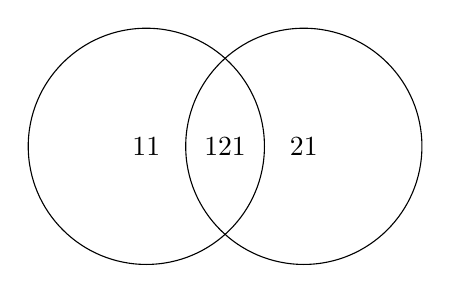
\begin{tikzpicture}
    \draw (-1,0) circle (1.5);
    \node at (-1,0) {$\re{1}{1}$};
    \draw ( 1,0) circle (1.5);
    \node at ( 1,0) {$\re{2}{1}$};
    \node at ( 0,0) {$\re{12}{1}$};
  \end{tikzpicture}
  \caption{The decomposition of an entropy vector of 2 variables in its atoms.}
  \label{fig:venn2}
\end{figure}

In the general case of entropy vectors of $n$ variables,
the $2^n-1$ vectors $\re{\Iis}{1}$ provides a base for the entropy space.
The matrix of the change of basis is unimodular and can be obtained as follows.
Suppose $h = \sum_{\Iis \in [n]\setminus\emptyset} \alpha_\Iis \re{\Iis}{1}$,
we have
\begin{align*}
  h_{\Jis} & = \sum_{\Iis \subseteq \Jis} \alpha_{\Iis}\\
  \alpha_{\Iis} & = \sum_{\Jis \subseteq \Iis} (-1)^{|\Iis\setminus \Jis|} (h_{[n]} - h_{[n]\setminus \Jis}).
\end{align*}
The first identity is easily obtained using the Venn diagram while the second identity can be obtained using the inclusion exclusion principle.

\begin{mydef}
  The \emph{cone of positive atoms} $\Ac$ is defined as
\[ \Ac = \{\, \sum_{\Iis \subseteq [n]\setminus\emptyset} \alpha_{\Iis} \re{\Iis}{1} \mid \alpha \geq 0 \,\}. \]
\end{mydef}

As we have seen, using the fact that $\Ec[1] = \R_+$, we have the following theorem.
\begin{mytheo}
  For any natural number $n$,
  \[ \Ac \subseteq \Ec. \]
\end{mytheo}

Since $\Ac \subseteq \Ec \subseteq \Pm$ and $\Ac[2] = \Pm[2]$, we have $\Ac[2] = \Ec[2] = \Pm[2]$.

\section{The entropic cone of 3 variables}
\label{sec:3var}
For 3 variables, the relation $\Ac[3] = \Pm[3]$ does not hold anymore.
The extreme rays of $\Pm[3]$ are the extreme rays of $\Ac[3]$ except for $\re{[3]}{2} \in \Pm[3]$ that is not $\Ac[3]$; see \figref{xor} for an illustration of $\re{[3]}{2}$.
This vector is entropic for $b=2$ as shown by \exemref{xor}.

\begin{myexem}
  \label{exem:xor}
  Consider the three independent coin tosses $X_1, X_2$ and $X_3 = X_1 \oplus X_2$ where $\oplus$ is the XOR operator.
  One can verify that the entropy vector of those random variables is $H_2(X) = \re{[3]}{2}$.
\end{myexem}

\begin{figure}[!ht]
  \centering
  \begin{subfigure}{0.48\textwidth}
    \centering
    \latthree{$h_1$ $h_2$ $h_{12}$ $h_3$ $h_{13}$ $h_{23}$ $h_{123}$}
    \caption{Lattice representation of an entropy vector $h$.}
    \label{fig:latex}
  \end{subfigure}
  \begin{subfigure}{0.45\textwidth}
    \centering
    \latthree{1 1 2 1 2 2 2}
    \caption{$\re{[3]}{2}$.}
    \label{fig:xor}
  \end{subfigure}
  \caption{Lattice representation of the entropy vector of $\Es[3]$.}
\end{figure}

Now, to conclude that ``$\Ec[3] = \Pm[3]$'', we would like to show that $\Ec$ is a cone.
That is, we would like to generalize \cororef{nonnegativeintegermult} and say that $\Ec$ is closed to multiplication with any nonnegative number.
However, this cannot be shown and $\Ec$ is not a cone for $n \geq 3$.

This is shown by \exemref{notcone} that is taken from \cite{zhang1997non}.

\begin{myexem}[\cite{zhang1997non}]
  \label{exem:notcone}
  Consider again $\re{[3]}{2}$.
  We can see that $\re{[3]}{2}$ is supported by the following dual entropy vector:
  $\di{1}{2}, \di{2}{3}, \di{3}{1}, \nd{1}{23}, \nd{2}{13}, \nd{3}{12}$.

  Consider a positive multiple $h = \lambda \re{[3]}{2}$ for some $\lambda > 0$.
  It is still supported by the same dual vectors so by \theoref{submodular}, $X_1, X_2, X_3$ are pairwise independent.
  Therefore,
  \begin{align*}
    p_{12} & = p_1 p_2\\
    p_{13} & = p_1 p_3\\
    p_{23} & = p_2 p_3.
  \end{align*}
  Moreover, by \theoref{nondecreasing},
  there exists functions $x_1(x_2, x_3), x_2(x_1, x_3), x_3(x_1, x_2)$ such that
  $p_{123} = p_{12}\delta_{x_3(x_1, x_2)} = p_{13}\delta_{x_2(x_1, x_3)} = p_{23}\delta_{x_1(x_2, x_3)}$.

  That is, for any $x_1, x_2, x_3$,
  \[ p_1(x_1)p_2(x_2)\delta_{x_3(x_1, x_2)}(x_3) = p_1(x_1)p_3(x_3)\delta_{x_2(x_1, x_3)}(x_2) = p_2(x_2)p_3(x_3)\delta_{x_1(x_2, x_3)}. \]
  We see with the first inequality that for any $x_2,x_3$, choosing $x_1 = x_1(x_2, x_3)$, we have
  \[ p_1(x_1)p_2(x_2) = p_1(x_1)p_3(x_3) \]
  hence $p_2(x_2) = p_3(x_3)$.
  That is, $X_1$, $X_2$ and $X_3$ are uniform and have alphabets of the same length.
  Therefore, the only entropy vectors of the ray of $\re{[3]}{2}$ that are entropic are the vectors
  \[ h = \log_b(m)\re{[3]}{2}. \]
  for a positive integer $m$.
\end{myexem}

We saw that the full dimensional polyhedron $\Ac$ is included in $\Ec$ but we have just seen that outside this polyhedron, $\Ec$ might not be a cone.
At this point one might be wondering how much ``porous'' $\Ec$ is.
It turns out that it is not that porous, there are just barely some ``scratch'' on the boundary.
More precisely, the closure of $\Ec$ is a convex cone (\theoref{convexcone}) and the relative interior of its closure is entropic (\theoref{relintcl}).

\begin{mylem}
  Consider two alphabets $\X_1, \X_2$ with $\X_1 \cap \X_2 = \emptyset$ and two \pmfs{}
  $p_1$ and $p_2$ respectively defined on $\X_1$ and $\X_2$.
  If $0 \leq \alpha \leq 1$, the \pmf
  \[
    p(x) =
    \begin{cases}
      \alpha p_1(x), & x \in \X_1\\
      (1-\alpha) p_2(x), & x \in \X_2
    \end{cases}
  \]
  has an entropy equal to
  \[ H_b(p) = \alpha H_b(p_1) + (1-\alpha) H_b(p_2) + \bH[b]{\alpha}. \]
\end{mylem}

\begin{mycoro}
  If $h, g \in \Ec$ then for any $0 \leq \alpha \leq 1$,
  $\alpha h + (1-\alpha) g + \bH[b]{\alpha} \re{[n]}{n} \in \Ec$.
\end{mycoro}

In particular, taking $g = 0$, and using \cororef{nonnegativeintegermult}, we have the following corollary.

\begin{mycoro}[{\cite[Lemma~4]{matus2007two}}]
  If $h \in \Ec$ then for any $\alpha, \beta > 0$,
  $\alpha h + \beta \re{[n]}{n} \in \Ec$.
\end{mycoro}

And finally, since we can take $\beta$ arbitrarily close to zero in the previous corollary.

\begin{mycoro}[{\cite[Corollary~2]{matus2007two}}]
  \label{coro:nonnegativemult}
  If $h \in \Ec$ then for any nonnegative number $\alpha$, $\alpha h \in \cl(\Ec)$.
\end{mycoro}

\cororef{nonnegativemult} and \lemref{add} implies the following theorem.

\begin{mytheo}
  \label{theo:convexcone}
  For integer $n$, $\cl(\Ec)$ is a convex cone.
\end{mytheo}

As mentioned earlier the only difference between $\cl(\Ec)$ and $\Ec$ is on the boundary of $\Ec$.

\begin{mytheo}
  \label{theo:relintcl}
  For any integer $n$,
  \[ \relint(\cl(\Ec)) \subseteq \Ec. \]
\end{mytheo}

This theorem is the consequence of the fact that $\Ec$ contains the full dimensional cone $\Ac$ as shown by the following lemma
that is taken from the proof of \cite[Theorem~1]{matus2007two}.

\begin{mylem}
  Consider a set $\Sset$.
  If $\cl(\Sset)$ is a convex cone, $\Sset$ contains a full dimensional cone $\Kis$ and $\Sset$ is close to addition then
  \[ \relint(\cl(\Sset)) \subseteq \Sset. \]
  \begin{proof}
    Suppose $x \in \relint(\cl(\Sset))$.
    Since $x$ is in the relative interior, $(x - \Kis) \cap \cl(\Sset)$ should not be empty.
    Since $\Kis$ is full dimensional, that means that $(x - \Kis) \cap \Sset$ is also nonempty.
    Let $y \in (x - \Kis) \cap \Sset$.
    Since $\Sset$ contains $\Kis$ and is closed to addition, $y + \Kis \subseteq \Sset$ and in particular $x \in \Sset$.
  \end{proof}
\end{mylem}





\section{The entropic cone of 4 variables}
\label{sec:4var}
The entropic cone of 4 variables has, in additions to $\Ac[3]$,
the extreme rays $\re{[3]}{2}, \re{[4]}{2}, \re{[4]}{3}$ and the three rays given by \figref{extremerays4} (up to symmetry).
The vector $\re{[3]}{2}$ is entropic, as seen in \secref{4var}.
The vector $\re{[4]}{3}$ is also entropic, it corresponds to $X_1, X_2, X_3$ being random coin tosses and $X_4 = X_1 \xor X_2 \xor X_3$.
The vector $\re{[4]}{2}$ is entropic too but it is less easy to see. %

\begin{figure}
  \centering
  \begin{subfigure}[b]{0.45\textwidth}
    \centering
    \latfour[1.1]{1 1 2 1 2 2 3 2 3 3 3 3 3 3 3}
    \caption{$X_1,X_2,X_3$ are independent coin tosses and
    $X_4 = (X_1 \oplus X_3, X_2 \oplus X_3)$.}%
    \label{fig:g43}
  \end{subfigure}\hfill
  \begin{subfigure}[b]{0.45\textwidth}
    \centering
    \latfour[1.1]{1 1 2 1 2 2 2 2 2 2 2 2 2 2 2}
    \caption{$X_1$ and $X_2$ are independent coin tosses,
    \label{fig:g42}
    $X_3 = X_1 \oplus X_2$ and $X_4 = (X_1,X_2)$.}
  \end{subfigure}
  \begin{subfigure}[b]{0.49\textwidth}
    \centering
    \latfour[1.1]{1 1 2 1 2 2 2 1 2 2 2 1 2 2 2}
    \caption{$X_1$ and $X_2$ are independent coin tosses and
    $X_4 = X_3 = X_1 \oplus X_2$.}
  \end{subfigure}
  \begin{subfigure}[b]{0.49\textwidth}
    \centering
    \latfour[1.1]{2 2 4 2 3 3 4 2 3 3 4 3 4 4 4}
    \caption{
      Non-entropic extreme ray of $\Pm[4]$. Its free expansion is the Vamos matroid \cite{vamos1968representation}. %
    }
    \label{fig:f12}
  \end{subfigure}
  \caption{Extreme rays of $\Ec[4]$ not expressible using the $\re{\Sset}{m}$ notation.}
  \label{fig:extremerays4}
\end{figure}

\section{Sculpting the Entropic Cone}
\label{sec:nsi}
In general, $\Ec \subseteq \Pm$.
We have seen that $\Ec[1] = \Pm[1], \Ec[2] = \Pm[2], \cEc[3] = \Pm[3]$ but as we will see, $\cEc[n] \subset \Pm[n]$ for $n \geq 4$.

The outer cone $\Pm$ is obtained using \theoref{nondecreasing} and \theoref{submodular}.
As $\Pm[4]$ is a strict superset of $\cEc[4]$,
that means that those theorems are not enough.
What have we missed ?
Do we need a new method to generate new entropic inequalities ?
It turns out that we can generate new inequalities using exactly the same method that we used to produce the outer bound $\Pm$.

\label{sec:sculpting}
\subsection{Generating non-shannon inequalities}
The method used to generate $\dPm$ is as follows:
\begin{enumerate}
  \item We consider an entropic vector $h$ and its \pmf{}. %
  \item We apply transformations on the \pmf{}.
  \item Then use the fact that $x \mapsto -\log(x)$ is nonnegative for $0 \leq x \leq 1$ using \propref{nonnegative} and the fact that $x \mapsto -\log(x)$ is convex using \propref{convex} to derive inequalities between the generated \pmfs.
    That is, we enforce $H_p(q) \geq 0$ and $D(p\|q) \geq 0$ between all pairs $p, q$.
  \item Then we look at the implications of those inequalities on the coordinates of the entropy vector $h$.
\end{enumerate}

We can consider different transformations:
\begin{description}
  \item[Marginalization]
    For $\Iis \subseteq [n]$, we can transform the \pmf{} $p$ to
    \[ \X_{\Iis} \to \R : x \mapsto p_{\Iis}(x_{\Iis}). \]
  \item[Contraction]
    For $\Iis \subseteq \Jis$ and some $x_{\Iis}$, we can transform the \pmf{} $p$ to
    \[ \X_{\Jis\setminus\Iis} \to \R : y \mapsto p_{\Jis|\Iis}(y|x_{\Iis}). \]
  \item[Inner-adhesivity]
    For $\Jis, \Kis$ with $\Iis = \Jis \cap \Kis$, we can transform the \pmf{} $p$ to
    \begin{equation}
      \label{eq:inneradhtransfo}
      \ia{\Jis}{\Kis}{\Iis}(p) \colon \X_{\Jis\cup\Kis} \to \R : x \mapsto \frac{p_{\Jis}(x_{\Jis})p_{\Kis}(x_{\Kis})}{p_{\Iis}(x_{\Iis})} = p_{\Jis|\Iis}(x_{\Jis}|x_{\Iis})p_{\Kis|\Iis}(x_{\Kis}|x_{\Iis})p_{\Iis}(x_{\Iis}).
    \end{equation}
    We denote $\ia{\Jis}{\Kis}{\Jis \cap \Kis}$ as $\iae{\Jis}{\Kis}$.
  \item[Self-adhesivity]
    For $\Iis \subseteq \Jis$, we can transform the \pmf{} $p$ to
    \begin{equation}
      \label{eq:selfadhtransfo}
      \sa{\Jis}{\Iis}(p) \colon \X \times \X_{\Jis\setminus\Iis} \to \R : x \mapsto \frac{p_{\Jis'}(x_{\Jis'})p_{\Jis}(x_{\Kis})}{p_{\Iis}(x_{\Iis})} = p_{\Jis'|\Iis}(x_{\Jis'}|x_{\Iis})p_{\Jis|\Iis}(x_{\Kis}|x_{\Iis})p_{\Iis}(x_{\Iis}).
    \end{equation}
    where $n' = n + |\Jis \setminus \Iis|$, $\Jis' = [n]$ and $\Kis = ([n'] \setminus [n]) \cup \Iis$
\end{description}

One could consider additional types of transformations.
For instance,
for $\Jis, \Kis, \Lis$ with $\Iis = \Jis \cap \Kis \cap \Lis$, we can transform the \pmf{} $p$ to
\[ \X_{\Jis\cup\Kis\cup\Lis} \to \R : x \mapsto p_{\Jis|\Iis}(x_{\Jis}|x_{\Iis})p_{\Kis|\Iis}(x_{\Kis}|x_{\Iis})p_{\Lis|\Iis}(x_{\Lis}|x_{\Iis})p_{\Iis}(x_{\Iis}). \]
However this transformation can be achieved by doing two inner-adhesivity transformations:
one with $(\Jis,\Kis\cup\Lis)$ and then one with $(\Jis\cup\Kis,\Lis)$.

We can see that \theoref{nondecreasing} was obtained using contraction and then \propref{nonnegative}
and \theoref{submodular} was obtained using inner-adhesivity and then \propref{convex}.

If we apply a transformation on a \pmf{} that is already a transformation of $p$,
we might not be able to express the resulting \pmf{} using $p$ without using summation.
For instance, suppose we do an inner-adhesivity transformation using the sets 12 and 13 with a \pmf{} $p$ of 3 variables:
$q = \iae{12}{13}(p) = p_{2|1}p_{3|1}p_1$.
If we marginalize $q$ on the second variable, it is $q_{13} = p_{13}$ but if we marginalize on the first variable,
it is
\[ \sum_{x_1 \in \X_1} q(x_1,x_2,x_3) = \sum_{x_1 \in \X_1} p_{2|1}(x_2|x_1)p_{3|1}(x_3|x_1)p_1(x_1) \]
but we cannot simplify it further.
This happens when we marginalize on a variable of $\Iis$ after an inner-adhesivity.
Suppose $q$ is obtained after applying an inner-adhesivity transformation on $p$ with $(\Jis,\Kis)$ of intersection $\Iis = \Jis \cap \Kis$.
Let $h$ (resp. $g$) be the entropic vector of $p$ (resp. $q$).
Suppose we want to compute $g_{\Lis}$ in terms of $h$.
\begin{itemize}
  \item If $\Lis \cap \Jis = \Iis$ or $\Lis \cap \Kis = \Iis$,
    then $g_{\Lis} = h_{\Lis}$.
  \item Otherwise, if $\Iis \subseteq \Lis$,
    \[ g_{\Lis} = h_{\Lis \cap \Jis} + h_{\Lis \cap \Kis} - h_{\Iis}. \]
    Note that the above equation gives $g_{\Lis} = h_{\Lis}$ if
    $\Lis \cap \Jis = \Iis$ or $\Lis \cap \Kis = \Iis$, it was only split in two cases for clarity.
  \item Otherwise, $q_{\Lis}$ is obtained from $q$ using marginalization on one of the variables in $\Iis$
    and $g_{\Lis}$ cannot be expressed in terms of $h$.
\end{itemize}
Even if some coordinates of $g$ cannot be expressed in terms of $g$, those coordinates can still be used to derive inequalities on $h$.

To illustrate this technique, we show in the following example how to prove the Zhang-Yeung inequality.

\begin{myexem}


One form of the Zhang-Yeung inequality is as follows:
\[ \la \ddi{3}{4}{1} + \ddi{3}{4}{2} + \di{1}{2} - \di{3}{4} + \ddi{3}{4}{5} + \ddi{5}{3}{4} + \ddi{4}{5}{3}, h \ra \geq 0 \]

Let $q = \ia{5}{12}{34} p$.
Let us abbreviate $H(p)$ with $p$.
The Zhang-Yeung inequality is:
\begin{align}
  \notag
  -p_{134} + \ia{3}{4}{1}p - p_{234} + \ia{3}{4}{2}p - p_{12} + \iae{1}{2}p - p_{32}\\
  \notag
  + \iae{3}{4}p - p_{345} + \ia{3}{4}{5}p - p_{345} + \ia{5}{3}{4}p - p_{345} + \ia{4}{5}{3}p & \geq 0\\
  \notag
  -p_{134} + p_{13} + p_{14} - p_1 - p_{234} + p_{23} + p_{24} - p_2 - p_{12} + p_1 + p_2 - p_{32} + p_3 + p_4\\
  \notag
  -p_{345} + p_{35} + p_{45} - p_5 - p_{345} + p_{45} + p_{34} - p_4 - p_{345} + p_{34} + p_{35} - p_3 & \geq 0\\
  \notag
  + p_{13} + p_{35} - p_3 + p_{14} + p_{45} - p_4\\
  \notag
  + p_{23} + p_{35} - p_3 + p_{24} + p_{45} - p_4\\
  \notag
  - p_5 {\color{green}- p_{134} - p_{345} + p_{34}} {\color{blue}- p_{234} - p_{345} + p_{34}} {\color{brown}- p_{1234} - p_{345} + p_{34}} + p_{1234} - p_{12} & \geq 0\\
  \notag
  + p_{13} + p_{35} - p_3 + p_{14} + p_{45} - p_4\\
  \notag
  + p_{23} + p_{35} - p_3 + p_{24} + p_{45} - p_4\\
  \notag
  - p_5 {\color{green}- q_{1345}} {\color{blue}- q_{2345}} {\color{brown}- q} + p_{1234} - p_{12} & \geq 0\\
  \notag
  - {\color{red}q_{135}} + p_{13} + p_{35} - p_3 - {\color{red}q_{145}} + p_{14} + p_{45} - p_4\\
  \notag
  - {\color{red}q_{235}} + p_{23} + p_{35} - p_3 - {\color{red}q_{245}} + p_{24} + p_{45} - p_4\\
  \notag
  - {\color{red}q_{125}} + {\color{red}p_{15}^1} + {\color{red}q_{25}} - p_5 - q_{1345} + {\color{red}q_{135}} + {\color{red}q_{145}} - {\color{red}q_{15}}\\
  \notag
  - q_{2345} + {\color{red}q_{235}} + {\color{red}q_{245}} - {\color{red}q_{25}} - q + {\color{red}q_{125}} + p_{1234} - p_{12} & \geq 0\\
  \notag
   - q_{135} + \ia{1}{5}{3}q - q_{145} + \ia{1}{5}{4}q - q_{235} + \ia{2}{5}{3}q - q_{245} + \ia{2}{5}{4}q\\
   \label{eq:nodiv}
   - q_{125} + \ia{1}{2}{5}q - q_{1345} + \ia{3}{4}{15}q - q_{2345} + \ia{3}{4}{25}q - q + \ia{34}{5}{12}q & \geq 0\\
  \notag
  D(q_{135} \| \ia{1}{5}{3}q) + D(q_{145} \| \ia{1}{5}{4}q) + D(q_{235} \| \ia{2}{5}{3}q) + D(q_{245} \| \ia{2}{5}{4}q)\\
   \label{eq:div}
  + D(q_{125} \| \ia{1}{2}{5}q) + D(q_{1345} \| \ia{3}{4}{15}q) + D(q_{2345} \| \ia{3}{4}{25}q) + D(q \| \ia{34}{5}{12}q) & \geq 0.
\end{align}

The last inequality is true by \propref{convex} so the Zhang-Yeung inequality is proven.

We used the following \pmf{} which are not expressible in terms of $p$ without summation.

\begin{align*}
  {\color{red}q_{135}} & = \sum_4 p_{5|34}p_{1|34}p_{34}\\
  {\color{red}q_{145}} & = \sum_3 p_{5|34}p_{1|34}p_{34}\\
  {\color{red}q_{235}} & = \sum_4 p_{5|34}p_{2|34}p_{34}\\
  {\color{red}q_{245}} & = \sum_3 p_{5|34}p_{2|34}p_{34}\\
  {\color{red}q_{125}} & = \sum_{34} p_{5|34}p_{12|34}p_{34}\\
  {\color{red}q_{15}} & = \sum_{34} p_{5|34}p_{1|34}p_{34}\\
  {\color{red}q_{25}} & = \sum_{34} p_{5|34}p_{2|34}p_{34}.
\end{align*}
\end{myexem}

The Zhang-Yeung inequality is a \emph{non-Shannon inequality} as it is not a consequence of the inequalities introduced in \secref{shannon}.
It was discovered by Zhang and Yeung in 1998~\cite{zhang1998characterization}.
The existence of this non-Shannon inequality shows that the inclusion $\cEc[n] \subset \Pm[n]$ is strict for $n \geq 4$.

\matus{} and Csirmaz~\cite{matus2013entropy} recently introduced a way to visualize the projection of a cut of approximations of the Entropic Cone of 4 random variables in 3 dimensions.
In this visualization, the polymatroid cone $\Pm[4]$ is the tetrahedron shown in \figref{tetra0zy}.

\begin{figure}[!ht]
  \centering
  \begin{subfigure}{0.48\textwidth}
    \centering
    \includegraphics[width=\textwidth]{tetra0pm.png}
    \caption{Polymatroid cone $\Pm[4]$.}
    \label{fig:tetra0pm}
  \end{subfigure}
  \begin{subfigure}{0.48\textwidth}
    \centering
    \includegraphics[width=\textwidth]{tetra0zy.png}
    \caption{The polymatroid cone $\Pm[4]$ cut by the Zhang-Yeung inequality.}
    \label{fig:tetra0zy}
  \end{subfigure}
  \caption{3D visualization of approximations of the Entropic Cone of 4 random variables.}
\end{figure}

\subsection{Formalizing the generation of non-shannon inequalities}
In the previous section, we have seen how to generate new inequalities in terms of transformation on the \pmf{}.
In practice, instead of looking at all those transformations together and all the possible succession of those transformations,
a specific transformation is chosen and we only keep its implication on the entropy space.
This may look conservative to only look at it from the entropy space but it makes it easier to reason about and to compute non-shannon inequalities.

The following theorems translate the invariance over \pmfs{} to the entropy space.

The contraction of a polymatroid is defined similarly to the contraction on matroid initially studied by Tutte \cite{tutte1958homotopyI,tutte1958homotopyII}; see also \cite[Section~4.3]{welsh2010matroid} or \cite[Section~3]{oxley2006matroid}.
\begin{mydef}[Contraction]
  The \emph{contraction} of a polymatroid $h$ onto $J \subset [n]$, denoted by $\contr{J}{h}$ is defined as
  \[ (\contr{J}{h})_{K} = h_{K \cap \Iis} - h_{\Iis}, \qquad K \subseteq J \]
  where $\Iis = [n] \setminus J$.
  It is also called the contraction of $\Iis$ from $h$ and denoted $h/\Iis$.
\end{mydef}

The following theorem is a consequence of \propref{diffcond} and \theoref{convexcone}.
\begin{mytheo}[{\cite[Lemma~1]{matus2013entropy}}]
  \label{theo:contraction}
  The family of cones $\cEc$ is closed under contraction.
\end{mytheo}

We define the following operators
\begin{align*}
  \ia{\Jis}{\Kis}{\Iis}(h) & = \{\, g \in \Es[n'] \mid \forall \Iis \subseteq \Lis \subseteq \Jis \cap \Kis, g_{\Lis} = h_{\Lis \cap \Jis} + h_{\Lis \cap \Kis} - h_{\Iis} \,\}, & \Iis & = \Jis \cap \Kis,\\
  \sa{\Jis}{\Iis}(h) & = \{\, g \in \Es[n'] \mid \forall \Iis \subseteq \Lis \subseteq \Jis' \cap \Kis, g_{\Lis} = h_{\Lis \cap \Jis'} + h_{\Lis \cap \Kis} - h_{\Iis} \,\}, & \Iis & \subseteq \Jis,
\end{align*}
where for inner-adhesivity, $n' = |\Jis\cup\Kis|$ and for self-adhesivity $n' = n + |\Jis \setminus \Iis|$, $\Jis' = [n]$ and $\Kis = ([n'] \setminus [n]) \cup \Iis$.

Again, we denote $\ia{\Jis}{\Kis}{\Jis \cap \Kis}$ as $\iae{\Jis}{\Kis}$.

\begin{mydef}
  We say that a family of sets $\Sset_n \subseteq \Es$ is \emph{inner-adhesive} if for any $n$, $x \in \Sset_n$ and $\Jis, \Kis \subseteq [n]$,
  there exists $y \in \Sset_{|\Jis\cup\Kis|}$ such that $y \in \iae{\Jis}{\Kis}(x)$ and
  we say that it is \emph{self-adhesive} if for any $n$, $x \in \Sset_n$ and $\Iis \subseteq \Jis \subseteq [n]$,
  there exists $y \in \Sset_{n + |\Jis \setminus \Iis|}$ such that $y \in \sa{\Jis}{\Iis}(x)$.
\end{mydef}

The following theorem is a consequence of equation~\eqref{eq:submodular}, and the transformation~\eqref{eq:inneradhtransfo} and~\eqref{eq:selfadhtransfo}.
\begin{mytheo}
  \label{theo:adh}
  The cone $\Ec$ is inner-adhesive and self-adhesive.
\end{mytheo}

An important numerical quantity, related with the geometric properties of $\Ec[4]$ is the \emph{Ingleton score} defined as
\begin{equation}
  \label{eq:ingleton}
  \ingsc \eqdef \inf_{0 \neq h \in \Ec[4]} \ingij{i}{j}(h)
\end{equation}
where $\ingij{i}{j}(h) = \la \ingsq{i}{j}, h \ra / h_{[n]}$ \cite[Definition~3]{dougherty2011non} and $\ingsq{i}{j}$ is the Ingleton dual entropy vector \cite{ingleton1971conditions}.
The Ingleton score of an approximation of the entropic cone of four variables is proportional to the ``height'' of the 3D visualization we introduced.
The Ingleton score of $\Pm[4]$ represented in \figref{tetra0pm} is $-\frac{1}{4}$ and the Ingleton score of the approximation represented in \figref{tetra0zy} is $-\frac{1}{6}$.

The current best lower bound on $\ingsc$ is equal to $-0.15789$~\cite{dougherty2011non}.
Upper bounds on $\ingsc$ can be obtained from exhibiting four jointly distributed variables for which the entropy vector has low Ingleton score.
The current best upper bound on $\ingsc$ is equal to $-0.09243$~\cite{matus2013entropy}.

The current best lower and upper bound are given respectively by the outer and inner approximation of $\Pm[4]$ illustrated by \figref{matcsir}.

\begin{figure}[!ht]
  \includegraphics[width=\textwidth]{matcsir.png}
  \caption{Outer~\cite{dougherty2011non} and inner~\cite{matus2013entropy} approximations of $\Pm[4]$.
  The figures comes from~\cite{matus2013entropy}.}
  \label{fig:matcsir}
\end{figure}









\section{Hierarchy of set programs}
\label{sec:optientropic}
We saw in \secref{nsi} with \theoref{adh} that the entropic cone is both inner-adhesive and self-adhesive. %
Those adhesive invariance are inclusion constraints of the form~\eqref{eq:algincl}
between entropic cones of different dimensions.
Consider the maximal cones included in the polymatroid cone $\Pm[i]$ for each number $i$ of random variables,
that are invariant under inner-adhesivity and self-adhesivity.
It is unknown whether these cones correspond to the entropic cones.
However, as the entropic cone is invariant under both inner-adhesivity and self-adhesivity,
these cones provide outer approximations of the entropic cones.
Moreover, these cones are the solution of the generic set program
with the countably infinite set variables $\mathcal{S}_1, \mathcal{S}_2, \ldots$ where
$\mathcal{S}_i$ corresponds to the outer approximation of the entropic
cone of $i$ random variables with
the inclusion constraints $\mathcal{S}_i \subseteq \Pm[i]$
and the inclusion constraints of the form~\eqref{eq:algincl} corresponding the
inner-adhesivity and self-adhesivity.

Consider the set program obtained by removing the variables $\mathcal{S}_i$ for $i > N$
and the constraints involving the sets that were removed.
The set programs for each $N$ form a hierarchy of set programs such that
the optimal solution for $\mathcal{S}_i$ corresponding to the set program for $N_1$
is included in the optimal solution for $\mathcal{S}_i$ corresponding to the set program for $N_2$ if $i < N_2 < N_1$.
That is, with increasing $N$, the outer approximation is closer to the entropic cone.

Solving the set program for polyhedral templates may need a prohibitive
number of halfspaces or rays in the representation as $\mathcal{S}_i$ has dimension $2^i - 1$.
However, for the purpose of optimization along a fixed direction in the entropic cone,
as discussed in \secref{dirobj}, we can circumvent this issue by only refining
the initial outer approximation $\Pm[i]$ where it matters for the optimization.
To verify this, we used \algoref{dirobj}
to find lower bounds for the Ingleton score and obtained the best known lower bound $-0.15789$ in under a minute.
The feasibility cuts generated to find this lower bound are represented in \figref{tetra0bound15789}.
Comparing \figref{tetra0bound15789} with the outer approximation of \figref{matcsir},
we see that, as expected, our approach only generates cuts close to the direction corresponding to the Ingleton score.

\begin{figure}[!ht]
  \centering
  \includegraphics[trim=6cm 2cm 6cm 7cm,clip,width=.8\textwidth]{tetra0bound15789.png}
  \caption{The polymatroid cone $\Pm[4]$ cut by the feasibility cuts uncovered to find the lower bound $-0.15789$ of the Ingleton score.}
  \label{fig:tetra0bound15789}
\end{figure}










\implementations{\jlpkg{EntropicCone}, \jlpkg{StructDualDynProg}.}

\section{Conclusion}

This chapter gives a glimpse of the potential of set programming for a given problem.
Until now, only polyhedral approximation of the entropic cone was considered.
However, when formulating the problem as a set program, we notice that a much wider range of methods can be utilized.
In view of the specificity of the problem, certain templates or methods seem more suitable:
as the entropic cone of 4 variables is piecewise linear in a significant part of the space,
piecewise semi-ellipsoidal sets or piecewise polysets seem appropriate.
If the entropic cone only needs to be closely approximated in specific directions then
polyhedral templates can be considered as well with \algoref{dirobj} to refine the approximation where it is relevant.

Using \algoref{dirobj}, we found the same lower bound on the Ingleton score than the
the one obtained in~\cite{dougherty2011non}.
Both methods use the polyhedral template so finding the same lower bound is not unexpected
but our methods finds it under a minute while hours of computations were needed in~\cite{dougherty2011non}.
Running \algoref{dirobj} longer should provide an improved lower bound but
the current implementation did not yet provide any.
Several implementation decisions have a significant impact on the time taken
to obtain the lower bounds:
\begin{itemize}
  \item when an infeasibility cut is found, should it be shared to other nodes for which it is valid (even if it may not be in a direction that matters for this node);
  \item should infeasibility cuts be kept forever or should old ones be dropped when their corresponding dual variables seem to repeatedly be zero (too many cuts may render the optimization too slow);
  \item when an infeasibility is found, should the ``early abortion'' described in \secref{dirobj} be applied ?
  \item as discussed in \secref{dirobj}, in which order should the elements in the
    set $I$ of \algoref{dirobj}.
\end{itemize}
We believe that if the impact of these choices should be analysed carefully,
a better lower bound should be obtainable in a reasonable time.

\clearemptydoublepage

\chapter{Conclusion}\label{chap:ccl}
In this thesis, we have explored the insights provided by analyzing set programs at the level of generic sets or generic convex sets.
We analyzed how these observations particularize to set programs for specific templates and how it affects their computability.

In \chapref{conv}, we introduced the different operations on sets that can be combined in the inclusion constraints of a set program.
We showed the properties related to these operations and the different representations of convex sets.
These results were then particularized for polyhedras, zonotopes, ellipsoids and specific subclasses of semialgebraic sets.

In \chapref{opti}, we detailed the optimization tools needed for
computing the sets of the different templates including for instance
the verification of membership of a point in a set and inclusion of
one sets in another set.

In \chapref{sys}, we introduced the different dynamical systems
and the condition for the invariance of sets for each one.
The classical algebraic methods to compute invariant sets were described.

In \chapref{setprog}, we describe set programs
using the operations defined in \chapref{conv}
and discuss the computation of solutions of such programs at the generic level depending on the operations used in the constraints.
We then translate this to each particular template.

In \chapref{stab}, we focus on the accuracy guarantees of the polyset template
for feasibility set programs with linear inclusion constraints.
The guarantee is based on the entropy of the language generated by the automaton underlying the constraint structure.
We also provide a rounding technique for generating infeasibility certificates
of the generic set program given infeasibility certificates of the
set program on polyset templates of a fixed degree.
We then show a way to approximate the set of constraints to remove in order to render
the set program feasible while maximizing the entropy of the resulting language.

In \chapref{mci}, the geometric approach to set programs developed in \chapref{setprog}
is used to provide a geometric interpretation for the semidefinite programs
used to compute ellipsoidal controlled invariant sets.
The crucial advantage of this geometric approach over the algebraic approach presented in \chapref{sys}
is the fact that it is carried out at the abstract level of generic convex sets.
Therefore, it directly provides semidefinite and sum-of-squares program
formulations for controlled invariant sets of any template that satisfy certain properties.
For instance, it provides a semidefinite program for computing controlled invariant piecewise semi-ellipsoidal sets and sum-of-squares program for sets with polynomial or even piecewise polynomial support function.
As highlighted in the introduction, the representation of
a set highly depends on the intended end-use.
To show this, we detail how the controlled invariant set can
be used in two different applications:
model predictive control and stochastic programming.

While the computation of invariant sets in Systems and Control is naturally formulated as a single set program,
we showed in \chapref{entropic} that the challenging problem of the approximation of the entropic cone can
be formulated as a hierarchy of set programs.
The results of \chapref{setprog} applied for this hierarchy of set programs provide
a novel method for optimizing on the entropic cone.

We hope this thesis has motivated the advantages of studying the generic set program at an abstract
level before focusing on a specific template.
Using \tabref{funop}, it allows to select the appropriate representation depending on the operations used in the set program in a template-independent manner.
Then, using \tabref{setop}, the appropriate templates can be selected and the performance of the several applicable templates
can be compared in order to select the most suitable one depending on the performance and accuracy of the computation
as well as the usability and quality for the intended end-use of the set.

\begin{table}[!ht]
  \centering
  \begin{tabular}{l|cccccc}
                         & $\cap$       & $\conv \cup$ &  $+$      & $\invsum$ &  $A$          & $A^{-1}$\\
    \hline
    Gauge function       & $\max$       & $\infconvol$ & $\invsum$ & $+$       &               & $\circ A$\\
    Support function     & $\infconvol$ & $\max$       & $+$       & $\invsum$ & $\circ A^\Tr$ &          \\
    Polar set            & $\conv \cup$ & $\cap$       & $\invsum$ & $+$       & $A^{-\Tr}$    & $A^{\Tr}$\\
  \end{tabular}
  \caption{Given an operation on convex sets specified by the column header,
  the corresponding operation on the gauge function, support function or polar set is provided in the table.%
  }
  \label{tab:funop}
\end{table}

\begin{table}[!ht]
  \centering
  \begin{tabular}{l|ccccccc}
    \textbf{Template}          & $\cap$ & $\conv \cup$ &  $+$   & $\invsum$ &  $A$   & $A^{-1}$  & $^\circ$\\
    \hline
    Polyhedra                  & \cmark & \cmark       & \cmark & \cmark    & \cmark & \cmark & \cmark\\
    Zonotopes                  & \xmark & \xmark       & \cmark & \xmark    & \cmark & \xmark & \xmark\\ %
    Ellipsoids                 & \xmark & \xmark       & \xmark & \xmark    & \cmark & \cmark & \cmark\\
    Polysets                   & \xmark & \xmark       & \xmark & \xmark    & \xmark & \cmark & \xmark\\ %
    Piecewise semi-ellipsoids  & \xmark & \xmark       & \xmark & \xmark    & \cmark & \cmark & \cmark\\
    Piecewise polysets         & \xmark & \xmark       & \xmark & \xmark    & \xmark & \cmark & \xmark\\ %
  \end{tabular}
  \caption{
  This table highlights the invariance of the different templates studied in this thesis
  under the operations preserving convexity that we consider.
  Each row represents a template and each column represents an operation.
  A \cmark{} symbol indicates that the template is invariant under the operation,
  a \xmark{} symbol indicates that it is not.
  A similar table can be found in \cite[Table~1]{kochdumper2020constrained}.}
  \label{tab:setop}
\end{table}

Many open questions remain to be investigated.
We only scratched the surface of the possible inclusion constraints with \eqref{eq:imageincl}, \eqref{eq:preimageincl}, \eqref{eq:projectpreimageincl} and \eqref{eq:algincl}
and many other possible inclusion constraints can be considered.
For instance, we could consider inclusions involving the other operations of
\tabref{setop} but also
inclusion of complements.
Note that the inclusion of $\mathcal{S}$ in the complement
of $\mathcal{T}$ is equivalent to the inclusion of $\mathcal{T}$ in the complement
of $\mathcal{S}$ and to $\mathcal{S} \cap \mathcal{T} = \emptyset$.
Moreover, the linear functions involved in \eqref{eq:imageincl}, \eqref{eq:preimageincl}, \eqref{eq:projectpreimageincl} and \eqref{eq:algincl} could be generalized to homogeneous functions or even \emph{generalized homogeneous functions}, see \cite{polyakov2020generalized} for a definition of generalized homogeneity.



\clearemptydoublepage

\printbibliography %


\end{document}
